\documentclass[11pt]{book} %10pt 11pt o 12pt permessi
%\documentclass{book}
\usepackage[T1]{fontenc} % codifica dei font
\usepackage[utf8]{inputenc} % lettere accentate da tastiera
\usepackage[italian]{babel} % lingua del documento
\usepackage{lipsum}

\usepackage{indentfirst} % indenta primo capoverso di paragrafo
\usepackage{microtype} % migliora riempimento righe - carica sempre
\usepackage{appendix}
\usepackage{emptypage}
\usepackage{tikz}
\usepackage{pgfplots}
\pgfplotsset{compat=1.17}
\usetikzlibrary{positioning}

%\usepackage[big]{layaureo} % con big nell'argomento bordi più larghi ancora
\usepackage[top=3cm,bottom=3cm,left=3.2cm,right=3.2cm,headsep=10pt, letterpaper]{geometry} % Page margins letterpaper

\usepackage{lipsum} % genera testo fittizio
\usepackage{comment}
\usepackage{quoting} % per le citazioni in display
\quotingsetup{font=small} % serve per mantenere lo stesso stile in tutte le citazioni

\usepackage{amsmath} % per la matematica
\usepackage{amssymb} % per la matematica
\usepackage{mathtools} % per valore assoluto e norma
\usepackage{braket} % per i comandi \Set e \Bra e simili
\usepackage{amsthm} % per teoremi e dimostrazioni

\usepackage[version=4]{mhchem} %CHIMICA

\usepackage{siunitx} % per unità di misura SI
\usepackage{textcomp} % SOLO SE si usano gradi Celsius

\usepackage{booktabs} % per tabelle
\usepackage{caption} % per tabelle
\usepackage{graphicx} % per figure
\usepackage{subfig} % per sottofigure

%%%%%%%%%%%%%% NEW THINGS %%%%%%%%%%%%%%%%%%%%%%%%%%%%%%%
\usepackage{xcolor} % Required for specifying colors by name
\definecolor{ocre}{RGB}{52,177,201} % Define the orange color used for highlighting throughout the book

% Font Settings
\usepackage{avant} % Use the Avantgarde font for headings
%\usepackage{times} % Use the Times font for headings
\usepackage{mathptmx} % Use the Adobe Times Roman as the default text font together with math symbols from the Sym­bol, Chancery and Com­puter Modern fonts

% Bibliography
%\usepackage[style=alphabetic,sorting=nyt,sortcites=true,autopunct=true,babel=hyphen,hyperref=true,abbreviate=false,backref=true,backend=biber]{biblatex}
%\addbibresource{bibliography.bib} % BibTeX bibliography file
%\defbibheading{bibempty}{}
%%%%%%%%%%%%%%%%%%%%%%%%%%%%%%%%%%%%%%%%%%%%%%%%%%%%%%%%%%%%%%

%\usepackage{hyperref} % metti alla fine
\usepackage{impostazioni} % per ultimo

%%%%%%%%%%%%%%%%%%%%%%%%%%%%%%%%%%%%%%%%%
% This is based on the Legrand Orange Book
% Structural Definitions File
%
% The original template (the Legrand Orange Book Template) can be found here --> http://www.latextemplates.com/template/the-legrand-orange-book
%
% Original author of the Legrand Orange Book Template::
% Mathias Legrand (legrand.mathias@gmail.com) with modifications by:
% Vel (vel@latextemplates.com)
%
% Original License:
% CC BY-NC-SA 3.0 (http://creativecommons.org/licenses/by-nc-sa/3.0/)
%
%%%%%%%%%%%%%%%%%%%%%%%%%%%%%%%%%%%%%%%%%
%----------------------------------------------------------------------------------------
%	VARIOUS REQUIRED PACKAGES
%----------------------------------------------------------------------------------------

%\usepackage{titlesec} % Allows customization of titles

%\usepackage{graphicx} % Required for including pictures
%\graphicspath{{Pictures/}} % Specifies the directory where pictures are stored

%\usepackage{lipsum} % Inserts dummy text

%\usepackage{tikz} % Required for drawing custom shapes

%\usepackage[english]{babel} % English language/hyphenation

\usepackage{enumitem} % Customize lists
\setlist{nolistsep} % Reduce spacing between bullet points and numbered lists

%\usepackage{booktabs} % Required for nicer horizontal rules in tables

\usepackage{eso-pic} % Required for specifying an image background in the title page

%----------------------------------------------------------------------------------------
%	MAIN TABLE OF CONTENTS
%----------------------------------------------------------------------------------------

\usepackage{titletoc} % Required for manipulating the table of contents

\contentsmargin{0cm} % Removes the default margin
% Chapter text styling
\titlecontents{chapter}[1.25cm] % Indentation
{\addvspace{15pt}\large\sffamily\bfseries} % Spacing and font options for chapters
{\color{ocre!60}\contentslabel[\Large\thecontentslabel]{1.25cm}\color{ocre}} % Chapter number
{}  
{\color{ocre!60}\normalsize\sffamily\bfseries\;\titlerule*[.5pc]{.}\;\thecontentspage} % Page number
% Section text styling
\titlecontents{section}[1.25cm] % Indentation
{\addvspace{5pt}\sffamily\bfseries} % Spacing and font options for sections
{\contentslabel[\thecontentslabel]{1.25cm}} % Section number
{}
{\sffamily\hfill\color{black}\thecontentspage} % Page number
[]
% Subsection text styling
\titlecontents{subsection}[1.25cm] % Indentation
{\addvspace{1pt}\sffamily\small} % Spacing and font options for subsections
{\contentslabel[\thecontentslabel]{1.25cm}} % Subsection number
{}
{\sffamily\;\titlerule*[.5pc]{.}\;\thecontentspage} % Page number
[] 

%----------------------------------------------------------------------------------------
%	MINI TABLE OF CONTENTS IN CHAPTER HEADS
%----------------------------------------------------------------------------------------

% Section text styling
\titlecontents{lsection}[0em] % Indendating
{\footnotesize\sffamily} % Font settings
{}
{}
{}

% Subsection text styling
\titlecontents{lsubsection}[.5em] % Indentation
{\normalfont\footnotesize\sffamily} % Font settings
{}
{}
{}
 
%----------------------------------------------------------------------------------------
%	PAGE HEADERS
%----------------------------------------------------------------------------------------

\usepackage{fancyhdr} % Required for header and footer configuration

\pagestyle{fancy}
\renewcommand{\chaptermark}[1]{\markboth{\sffamily\normalsize\bfseries\chaptername\ \thechapter.\ #1}{}} % Chapter text font settings
\renewcommand{\sectionmark}[1]{\markright{\sffamily\normalsize\thesection\hspace{5pt}#1}{}} % Section text font settings
\fancyhf{} \fancyhead[LE,RO]{\sffamily\normalsize\thepage} % Font setting for the page number in the header
\fancyhead[LO]{\rightmark} % Print the nearest section name on the left side of odd pages
\fancyhead[RE]{\leftmark} % Print the current chapter name on the right side of even pages
\renewcommand{\headrulewidth}{0.5pt} % Width of the rule under the header
\addtolength{\headheight}{2.5pt} % Increase the spacing around the header slightly
\renewcommand{\footrulewidth}{0pt} % Removes the rule in the footer
\fancypagestyle{plain}{\fancyhead{}\renewcommand{\headrulewidth}{0pt}} % Style for when a plain pagestyle is specified

% Removes the header from odd empty pages at the end of chapters
\makeatletter
\renewcommand{\cleardoublepage}{
\clearpage\ifodd\c@page\else
\hbox{}
\vspace*{\fill}
\thispagestyle{empty}
\newpage
\fi}

%----------------------------------------------------------------------------------------
%	THEOREM STYLES
%----------------------------------------------------------------------------------------

\usepackage{amsmath,amsfonts,amssymb,amsthm} % For math equations, theorems, symbols, etc

\newcommand{\intoo}[2]{\mathopen{]}#1\,;#2\mathclose{[}}
\newcommand{\ud}{\mathop{\mathrm{{}d}}\mathopen{}}
\newcommand{\intff}[2]{\mathopen{[}#1\,;#2\mathclose{]}}
\newtheorem{notation}{Notation}[chapter]

%%%%%%%%%%%%%%%%%%%%%%%%%%%%%%%%%%%%%%%%%%%%%%%%%%%%%%%%%%%%%%%%%%%%%%%%%%%
%%%%%%%%%%%%%%%%%%%% dedicated to boxed/framed environements %%%%%%%%%%%%%%
%%%%%%%%%%%%%%%%%%%%%%%%%%%%%%%%%%%%%%%%%%%%%%%%%%%%%%%%%%%%%%%%%%%%%%%%%%%
\newtheoremstyle{ocrenumbox}% % Theorem style name
{0pt}% Space above
{0pt}% Space below
{\normalfont}% % Body font
{}% Indent amount
{\small\bf\sffamily\color{ocre}}% % Theorem head font
{\;}% Punctuation after theorem head
{0.25em}% Space after theorem head
{\small\sffamily\color{ocre}\thmname{#1}\nobreakspace\thmnumber{\@ifnotempty{#1}{}\@upn{#2}}% Theorem text (e.g. Theorem 2.1)
\thmnote{\nobreakspace\the\thm@notefont\sffamily\bfseries\color{black}---\nobreakspace#3.}} % Optional theorem note
\renewcommand{\qedsymbol}{$\blacksquare$}% Optional qed square

\newtheoremstyle{blacknumex}% Theorem style name
{5pt}% Space above
{5pt}% Space below
{\normalfont}% Body font
{} % Indent amount
{\small\bf\sffamily}% Theorem head font
{\;}% Punctuation after theorem head
{0.25em}% Space after theorem head
{\small\sffamily{\tiny\ensuremath{\blacksquare}}\nobreakspace\thmname{#1}\nobreakspace\thmnumber{\@ifnotempty{#1}{}\@upn{#2}}% Theorem text (e.g. Theorem 2.1)
\thmnote{\nobreakspace\the\thm@notefont\sffamily\bfseries---\nobreakspace#3.}}% Optional theorem note

\newtheoremstyle{blacknumbox} % Theorem style name
{0pt}% Space above
{0pt}% Space below
{\normalfont}% Body font
{}% Indent amount
{\small\bf\sffamily}% Theorem head font
{\;}% Punctuation after theorem head
{0.25em}% Space after theorem head
{\small\sffamily\thmname{#1}\nobreakspace\thmnumber{\@ifnotempty{#1}{}\@upn{#2}}% Theorem text (e.g. Theorem 2.1)
\thmnote{\nobreakspace\the\thm@notefont\sffamily\bfseries---\nobreakspace#3.}}% Optional theorem note

%%%%%%%%%%%%%%%%%%%%%%%%%%%%%%%%%%%%%%%%%%%%%%%%%%%%%%%%%%%%%%%%%%%%%%%%%%%
%%%%%%%%%%%%% dedicated to non-boxed/non-framed environements %%%%%%%%%%%%%
%%%%%%%%%%%%%%%%%%%%%%%%%%%%%%%%%%%%%%%%%%%%%%%%%%%%%%%%%%%%%%%%%%%%%%%%%%%
\newtheoremstyle{ocrenum}% % Theorem style name
{5pt}% Space above
{5pt}% Space below
{\normalfont}% % Body font
{}% Indent amount
{\small\bf\sffamily\color{ocre}}% % Theorem head font
{\;}% Punctuation after theorem head
{0.25em}% Space after theorem head
{\small\sffamily\color{ocre}\thmname{#1}\nobreakspace\thmnumber{\@ifnotempty{#1}{}\@upn{#2}}% Theorem text (e.g. Theorem 2.1)
\thmnote{\nobreakspace\the\thm@notefont\sffamily\bfseries\color{black}---\nobreakspace#3.}} % Optional theorem note
\renewcommand{\qedsymbol}{$\blacksquare$}% Optional qed square
\makeatother

% Defines the theorem text style for each type of theorem to one of the three styles above
\newcounter{dummy} 
\numberwithin{dummy}{section}
\theoremstyle{ocrenumbox}
\newtheorem{theoremeT}[dummy]{Theorem}
\newtheorem{problem}{Problem}[chapter]
\newtheorem{exerciseT}{Exercise}[chapter]
\theoremstyle{blacknumex}
\newtheorem{exampleT}{Example}[chapter]
\theoremstyle{blacknumbox}
\newtheorem{vocabulary}{Vocabulary}[chapter]
\newtheorem{definitionT}{Definition}[section]
\newtheorem{corollaryT}[dummy]{Corollary}
\theoremstyle{ocrenum}
\newtheorem{proposition}[dummy]{Proposition}

%----------------------------------------------------------------------------------------
%	DEFINITION OF COLORED BOXES
%----------------------------------------------------------------------------------------

\RequirePackage[framemethod=default]{mdframed} % Required for creating the theorem, definition, exercise and corollary boxes

% Theorem box
\newmdenv[skipabove=7pt,
skipbelow=7pt,
backgroundcolor=black!5,
linecolor=ocre,
innerleftmargin=5pt,
innerrightmargin=5pt,
innertopmargin=5pt,
leftmargin=0cm,
rightmargin=0cm,
innerbottommargin=5pt]{tBox}

% Exercise box	  
\newmdenv[skipabove=7pt,
skipbelow=7pt,
rightline=false,
leftline=true,
topline=false,
bottomline=false,
backgroundcolor=ocre!10,
linecolor=ocre,
innerleftmargin=5pt,
innerrightmargin=5pt,
innertopmargin=5pt,
innerbottommargin=5pt,
leftmargin=0cm,
rightmargin=0cm,
linewidth=4pt]{eBox}	

% Definition box
\newmdenv[skipabove=7pt,
skipbelow=7pt,
rightline=false,
leftline=true,
topline=false,
bottomline=false,
linecolor=ocre,
innerleftmargin=5pt,
innerrightmargin=5pt,
innertopmargin=0pt,
leftmargin=0cm,
rightmargin=0cm,
linewidth=4pt,
innerbottommargin=0pt]{dBox}	

% Corollary box
\newmdenv[skipabove=7pt,
skipbelow=7pt,
rightline=false,
leftline=true,
topline=false,
bottomline=false,
linecolor=gray,
backgroundcolor=black!5,
innerleftmargin=5pt,
innerrightmargin=5pt,
innertopmargin=5pt,
leftmargin=0cm,
rightmargin=0cm,
linewidth=4pt,
innerbottommargin=5pt]{cBox}

% Creates an environment for each type of theorem and assigns it a theorem text style from the "Theorem Styles" section above and a colored box from above
\newenvironment{theorem}{\begin{tBox}\begin{theoremeT}}{\end{theoremeT}\end{tBox}}
\newenvironment{exercise}{\begin{eBox}\begin{exerciseT}}{\hfill{\color{ocre}\tiny\ensuremath{\blacksquare}}\end{exerciseT}\end{eBox}}				  
\newenvironment{definition}{\begin{dBox}\begin{definitionT}}{\end{definitionT}\end{dBox}}	
\newenvironment{example}{\begin{exampleT}}{\hfill{\tiny\ensuremath{\blacksquare}}\end{exampleT}}		
\newenvironment{corollary}{\begin{cBox}\begin{corollaryT}}{\end{corollaryT}\end{cBox}}	

%----------------------------------------------------------------------------------------
%	REMARK ENVIRONMENT
%----------------------------------------------------------------------------------------

\newenvironment{remark}{\par\vspace{10pt}\small % Vertical white space above the remark and smaller font size
\begin{list}{}{
\leftmargin=35pt % Indentation on the left
\rightmargin=25pt}\item\ignorespaces % Indentation on the right
\makebox[-2.5pt]{\begin{tikzpicture}[overlay]
\node[draw=ocre!60,line width=1pt,circle,fill=ocre!25,font=\sffamily\bfseries,inner sep=2pt,outer sep=0pt] at (-15pt,0pt){\textcolor{ocre}{R}};\end{tikzpicture}} % Orange R in a circle
\advance\baselineskip -1pt}{\end{list}\vskip5pt} % Tighter line spacing and white space after remark

%----------------------------------------------------------------------------------------
%	SECTION NUMBERING IN THE MARGIN
%----------------------------------------------------------------------------------------

\makeatletter
\renewcommand{\@seccntformat}[1]{\llap{\textcolor{ocre}{\csname the#1\endcsname}\hspace{1em}}}                    
\renewcommand{\section}{\@startsection{section}{1}{\z@}
{-4ex \@plus -1ex \@minus -.4ex}
{1ex \@plus.2ex }
{\normalfont\large\sffamily\bfseries}}
\renewcommand{\subsection}{\@startsection {subsection}{2}{\z@}
{-3ex \@plus -0.1ex \@minus -.4ex}
{0.5ex \@plus.2ex }
{\normalfont\sffamily\bfseries}}
\renewcommand{\subsubsection}{\@startsection {subsubsection}{3}{\z@}
{-2ex \@plus -0.1ex \@minus -.2ex}
{.2ex \@plus.2ex }
{\normalfont\small\sffamily\bfseries}}                        
\renewcommand\paragraph{\@startsection{paragraph}{4}{\z@}
{-2ex \@plus-.2ex \@minus .2ex}
{.1ex}
{\normalfont\small\sffamily\bfseries}}

%----------------------------------------------------------------------------------------
%	HYPERLINKS IN THE DOCUMENTS
%----------------------------------------------------------------------------------------

% For an unclear reason, the package should be loaded now and not later
\usepackage{hyperref}
\hypersetup{hidelinks,backref=true,pagebackref=true,hyperindex=true,colorlinks=true, breaklinks=true,urlcolor= ocre,bookmarks=true,bookmarksopen=false,pdftitle={Title},pdfauthor={Author}}

%----------------------------------------------------------------------------------------
%	CHAPTER HEADINGS
%----------------------------------------------------------------------------------------

% The set-up below should be (sadly) manually adapted to the overall margin page septup controlled by the geometry package loaded in the main.tex document. It is possible to implement below the dimensions used in the goemetry package (top,bottom,left,right)... TO BE DONE

\newcommand{\thechapterimage}{}
\newcommand{\chapterimage}[1]{\renewcommand{\thechapterimage}{#1}}

% Numbered chapters with mini tableofcontents
\def\thechapter{\arabic{chapter}}
\def\@makechapterhead#1{
\thispagestyle{empty}
{\centering \normalfont\sffamily
\ifnum \c@secnumdepth >\m@ne
\if@mainmatter
\startcontents
\begin{tikzpicture}[remember picture,overlay]
\node at (current page.north west)
{\begin{tikzpicture}[remember picture,overlay]
\node[anchor=north west,inner sep=0pt] at (0,0) {\includegraphics[width=\paperwidth]{\thechapterimage}};
%%%%%%%%%%%%%%%%%%%%%%%%%%%%%%%%%%%%%%%%%%%%%%%%%%%%%%%%%%%%%%%%%%%%%%%%%%%%%%%%%%%%%
% Commenting the 3 lines below removes the small contents box in the chapter heading
%\fill[color=ocre!10!white,opacity=.6] (1cm,0) rectangle (8cm,-7cm);
%\node[anchor=north west] at (1.1cm,.35cm) {\parbox[t][8cm][t]{6.5cm}{\huge\bfseries\flushleft \printcontents{l}{1}{\setcounter{tocdepth}{2}}}};
\draw[anchor=west] (5cm,-9cm) node [rounded corners=20pt,fill=ocre!10!white,text opacity=1,draw=ocre,draw opacity=1,line width=1.5pt,fill opacity=.6,inner sep=12pt]{\huge\sffamily\bfseries\textcolor{black}{\thechapter. #1\strut\makebox[22cm]{}}};
%%%%%%%%%%%%%%%%%%%%%%%%%%%%%%%%%%%%%%%%%%%%%%%%%%%%%%%%%%%%%%%%%%%%%%%%%%%%%%%%%%%%%
\end{tikzpicture}};
\end{tikzpicture}}
\par\vspace*{230\p@}
\fi
\fi}

% Unnumbered chapters without mini tableofcontents (could be added though) 
\def\@makeschapterhead#1{
\thispagestyle{empty}
{\centering \normalfont\sffamily
\ifnum \c@secnumdepth >\m@ne
\if@mainmatter
\begin{tikzpicture}[remember picture,overlay]
\node at (current page.north west)
{\begin{tikzpicture}[remember picture,overlay]
\node[anchor=north west,inner sep=0pt] at (0,0) {\includegraphics[width=\paperwidth]{\thechapterimage}};
\draw[anchor=west] (5cm,-9cm) node [rounded corners=20pt,fill=ocre!10!white,fill opacity=.6,inner sep=12pt,text opacity=1,draw=ocre,draw opacity=1,line width=1.5pt]{\huge\sffamily\bfseries\textcolor{black}{#1\strut\makebox[22cm]{}}};
\end{tikzpicture}};
\end{tikzpicture}}
\par\vspace*{230\p@}
\fi
\fi
}
\makeatother % Insert the commands.tex file which contains the majority of the structure behind the template

\begin{document}

\title{Appunti di Astrofisica}

%----------------------------------------------------------------------------------------
%	TITLE PAGE
%----------------------------------------------------------------------------------------

\begingroup
\thispagestyle{empty}
\AddToShipoutPicture*{\put(0,0){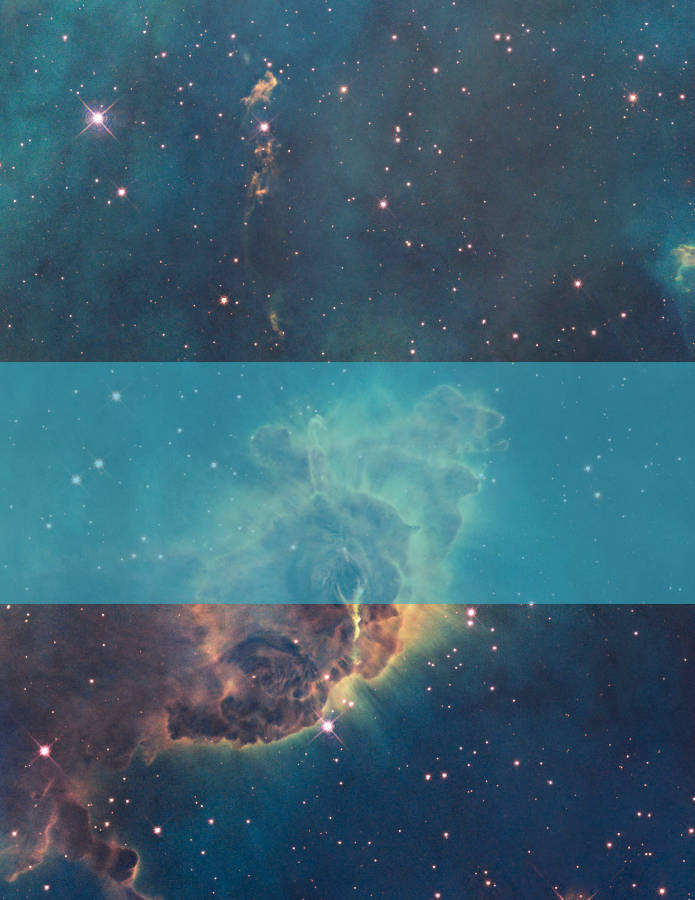
\includegraphics[scale=1.25]{cover/esahubble}}} % Image background
\centering
\vspace*{5cm}
\par\normalfont\fontsize{35}{35}\sffamily\selectfont
\textbf{Appunti di Astrofisica}\\
{\LARGE Corso della prof.ssa B. Lanzoni~- A.A. $2022/2023$}\par % Book title
\vspace*{1cm}
{\Huge G.~Oancia, S.~Coli, L.~Calandra~Buonaura, A.~D'Amico}\par % Author name
\endgroup

%----------------------------------------------------------------------------------------
%	COPYRIGHT PAGE
%----------------------------------------------------------------------------------------

\newpage
~\vfill
\thispagestyle{empty}

%\noindent Copyright \copyright\ 2014 Andrea Hidalgo\\ % Copyright notice

\noindent \textsc{Università di Bologna}\\

\noindent \textsc{github.com/gianchix/appunti-astrofisica}\\ % URL

\noindent Prima Stesura\\ % License information

\noindent \textit{Prima pubblicazione, Gennaio 2023} % Printing/edition date

%----------------------------------------------------------------------------------------
%	PREFACE
%----------------------------------------------------------------------------------------

\newpage
\thispagestyle{empty}
{\noindent \bfseries \Huge \prefacename}
       \begin{center}
            % \phantomsection \addcontentsline{toc}{chapter}{\prefacename} % enable this if you want to put the preface in the table of contents
            \thispagestyle{plain}
            
            \lipsum[3]

            \lipsum[3]

            \lipsum[3]
        \end{center}%
    {\vspace*{\stretch{5}}}


%----------------------------------------------------------------------------------------
%	TABLE OF CONTENTS
%----------------------------------------------------------------------------------------

\chapterimage{cover/head1.png} % Table of contents heading image

\pagestyle{empty} % No headers

\hypersetup{linkcolor = black}
\tableofcontents % Print the table of contents itself

\cleardoublepage % Forces the first chapter to start on an odd page so it's on the right

\pagestyle{fancy} % Print headers again
\hypersetup{linkcolor = ocre}

%----------------------------------------------------------------------------------------
%	CHAPTER 1
%----------------------------------------------------------------------------------------


\mainmatter

\begin{comment}
\chapterimage{cover/head2.png} % Chapter heading image
\chapter{Setting the stage}
\section{Introduzione}\label{sec:introduzione}
Come per ogni ambito della fisica, anche per l'\emph{astrofisica} è necessario avere in mente gli ordini di grandezza con cui si lavora e gli oggetti di studio. Nella tab.~\ref{tab:ordini-grandezza-sole-vialattea} sono riportate alcune grandezze riferite al nostro Sole e alla Via Lattea. A causa delle scale spaziali e temporali enormi rispetto a quella umana, risulta ovvio che non è possibile riprodurre le strutture cosmiche in laboratorio, andare su di esse per prendere delle misure dirette, oppure seguirne la loro evoluzione istante per istante. Dunque, è necessario uno studio \emph{indiretto}, che avvenga analizzando la radiazione che riceviamo, che proviene necessariamente dal passato. In prima approssimazione, possiamo ritenere che essa sia stata emessa $\Delta t = D / c$ tempo fa, con $D$ distanza della sorgente e $c$ velocità della luce nel vuoto. Un altro limite delle osservazioni astrofisiche consiste nel non avere accesso alla terza dimensione, ovvero alla profondità rispetto alla linea di vista. Inoltre, è necessario un \emph{approccio statistico} per comprendere i processi evolutivi, cercando, in prima istanza, di raggruppare oggetti simili, i quali presumibilmente abbiamo la stessa età. Ovviamente l'astrofisica utilizza le \emph{leggi della fisica} per interpretare i dati osservativi e avanzare predizioni teoriche, tramite \emph{modelli} e \emph{simulazioni}.

\begin{table}
    \caption{Ordini di grandezza riferiti al Sole e alla Via Lattea.}
    \label{tab:ordini-grandezza-sole-vialattea}
    \centering
    \begin{tabular}{lll}
    \toprule
    Grandezza & Sole & Via Lattea  \\
    \midrule
    Raggio (\si{cm}) & $\sim \SI{6.7e10}{}$ & $\sim \SI{8e22}{}$ \\
    Massa (\si{g}) & $\sim \SI{2e33}{}$    & $\sim \SI{e45}{}$    \\
    Età (\si{s}) & $\sim \SI{1.4e17}{}$  & $\sim \SI{3.8e17}{}$  \\
    Distanza da noi (\si{cm}) & $\sim \SI{1.5e13}{}$  & $\sim \SI{2.5e22}{}$  \\
    \bottomrule
    \end{tabular}
\end{table}
\input{capitoli/setting/unità.tex}


\chapterimage{cover/head3.png}
\chapter{Meccanismi di emissione}
\section{Introduzione all'astrofisica osservativa}\label{sec:astrofisica-osservativa}
Come introdotto nel paragrafo~\ref{sec:introduzione}, l'astrofisica studia le strutture cosmiche in maniera indiretta attraverso la radiazione che raccogliamo con i telescopi e altri strumenti. In particolare, osservando a bande diverse, posso estrapolare informazioni quantitative dalla misura della radiazione. Si tenga tuttavia a mente che la radiazione che riceviamo dipende sia dai processi fisiche che l'hanno generata che dai processi fisici che ha subito nel tragitto tra sorgente e osservatore.

Primo problema dell'osservazione è il così detto \emph{assorbimento atmosferico}. Infatti, non tutta la radiazione emessa dagli oggetti astrofisici riesce a raggiungere la superficie terrestre. Arrivano il vicino ultravioletto, il vicino infrarosso e le onde radio e visibili, mentre il resto della radiazione non arriva a terra perché viene assorbita dall'atmosfera. È dunque necessario osservare con telescopi spaziali in orbita fuori dall'atmosfera terrestre. Un altro problema che si riscontra è quello del \emph{seeing}, secondo il quale le particelle di vapor acqueo dell'atmosfera creano una turbolenza che ha la conseguenza di sfocare le immagini acquisite dai telescopi. Per questo motivo tendiamo a osservare in posti poco umidi, come il Cile o le Hawaii. Senza tecniche per correggere tale problema sarebbe inutile cercare di avere telescopi di diametro maggiore per avere una maggior qualità dell'immagine. Se guardo una stella, l'immagine risulta un disco sulla lente, mentre se c'è turbolenza ho una immagine distorta e che si muove. Un'immagine affetta dal problema del seeing si dice \emph{seeing-limited}. Si chiama inoltre \emph{diffraction-limited} la minore distanza angolare che si può risolvere, essa equivale a
\[
    \theta = 1.22 \frac{\lambda}{D}
\]
dove $\lambda$ è la lunghezza d'onda dell'onda incidente sulla lente di diametro $D$. Si può notare che, se fossimo in grado di risolvere il problema del seeing, aumentando il diametro della lente saremmo in grado di diminuire il potere risolutivo e quindi potremmo risolvere oggetti più vicini. Fortunatamente, la tecnologia attuale offre la possibilità di correggere il problema del seeing attraverso l'utilizzo di \emph{ottiche adattive}. Nella figura~\ref{fig:ottiche-adattive} si spiega il loro funzionamento. 

\begin{figure}
\centering
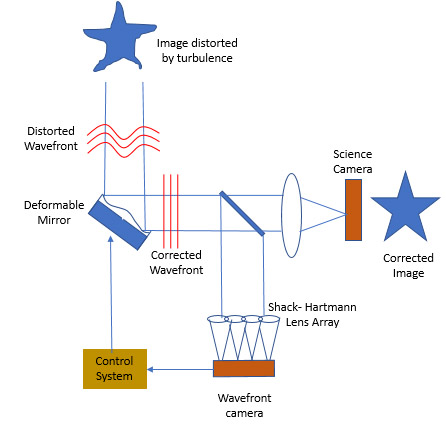
\includegraphics[width=0.4\textwidth]{immagini/ottiche-adattive.png}
\caption{Principio di funzionamento delle ottiche adattive. Un fronte d’onda distorto incide su uno specchio deformabile (con pistoni idraulici che si allungano o contraggono), la luce passa attraverso un sistema che la manda a un sistema (waveform camera) che controlla se l’immagine della stella è soggetta a turbolenza oppure no, se è distorta (ovvero soggetta a turbolenza), dice ai pistoncini idraulici come deformare lo specchio iniziale per annullare tale effetto.}
\label{fig:ottiche-adattive}
\end{figure}

Per calcolare la deformazione da applicare alla lente per correggere il problema del seeing, si utilizza una \emph{stella guida}, che deve essere una stella molto brillante. Siccome non sempre è presente una stella molto brillante per effettuare la calibrazione, si utilizza una \emph{stella laser}, ovvero i telescopi sparano fasci laser brillanti che simulano la presenza di una stella brillante attraverso l'eccitazione di atomi di sodio a $\SI{90}{km}$ di altitudine. Un altro modo per evitare il seeing è banalmente evitare l'atmosfera terrestre, dunque utilizzare telescopi spaziali, che sono solamente diffraction-limited.

Si vuole, infine, sottolineare la differenza tra un telescopio e i suoi strumenti a bordo: ciascun telescopio, infatti, ha diversi strumenti a bordo. Questi si dividono in due categorie particolari: le \emph{photometric cameras}, utilizzate per l'imaging o la spettroscopia, e gli \emph{spettrografi}, utilizzati per la spettrografia, ovvero per misurare lo spettro della radiazione, che può essere in assorbimento o in emissione.
\section{Equazione del trasporto radiativo}\label{sec:intro-trasporto-radiativo}
Come anticipato nel paragrafo~\ref{sec:astrofisica-osservativa}, per poter interpretare in maniera corrette le misure di radiazione, è necessario studiare i meccanismi d'interazione tra la radiazione e la materia. Le cause principali di tale interazione sono l'\emph{assorbimento}, lo \emph{scattering}\footnote{Lo scattering è la deviazione rispetto alla direzione di propagazione originale} e l'\emph{emissione}. Questi fenomeni variano a seconda della \emph{frequenza} e questo è il motivo per cui osservare a frequenze diverse porta a informazioni diverse.

L'\emph{equazione del trasporto radiativo} descrive il trasporto di radiazione da parte dei fotoni. Non è l'unico meccanismo di trasporto ma è il più comune nell'universo. In particolare, l'equazione dice come varia l'intensità della radiazione a causa dell'interazione tra la radiazione e la materia. Prima di ricavare l'equazione è necessario introdurre alcune grandezze indispensabili per indicare le energie.

\subsection{Intensità specifica o brillanza}\label{sec:intensità}
Dato un campo di radiazione, l'intensità specifica $I_\nu$ lungo la direzione $k$, in un punto qualsiasi $P$ del campo, è la quantità di energia che, in un intervallo di tempo $\ud t$ e nell'intervallo di frequenze $\ud \nu$, attraversa una superficie infinitesima perpendicolare alla direzione $k$ ($\ud A_\perp$), entro un angolo solido elementare $\ud \Omega$:
\begin{equation}\label{eq:intensità}
    I_\nu = \frac{\ud E}{\ud t \ud \nu \ud A \ud \Omega \cos{\theta}} \quad \bigl[\si{erg.s^{-1}.cm^{-2}.Hz^{-1}.sr^{-1}}\bigr]
\end{equation}
dove $\theta$ è l'angolo tra la normale a $\ud A$ e la direzione $k$, ovvero posso scrivere: $\ud A_\perp = \ud A \cos{\theta}$. Si guardi la figura~\ref{fig:intensità-specifica}.

\begin{figure}
\centering
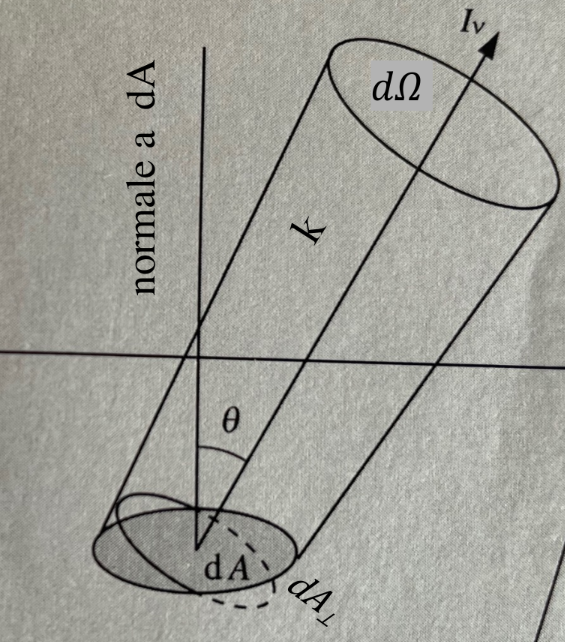
\includegraphics[width=0.25\textwidth]{immagini/intensita-specifica.png}
\caption{Definizione di intensità specifica. $\ud A$ è un'area infinitesima sulla superficie della stella, $P$ è il punto della superficie della stella, $k$ è il versore rispetto al quale definisco l'intensità e $\ud A_\perp = \ud A \cos{\theta}$. La radiazione è portata da un fascio di fotoni, quindi devo considerare un tronco di angolo solido $\ud \Omega$, in cui $\ud A$ rappresenta la sezione del fascio.}
\label{fig:intensità-specifica}
\end{figure}

Si tratta di una proprietà \emph{intrinseca} del campo di radiazione, ovvero della sorgente, ed è definita per unità di frequenza o equivalentemente di lunghezza d'onda.

Si ricordi, inoltre, che il differenziale di angolo solido si scrive:
\begin{equation}\label{eq:angolo-solido}
    \ud \Omega = \sin{\theta} \ud \theta \ud \phi
\end{equation}

Più avanti vedremo uno spettro o \emph{distribuzione spettrale di energia (SED)}, rappresentante la dipendenza dell'intensità dalla lunghezza d'onda (equivalentemente dalla frequenza). 

\subsection{Luminosità}\label{sec:luminosità}
La \emph{luminosità bolometrica} ($L$) di una sorgente è definita come la quantità di energia totale emessa dalla sorgente nell'unità di tempo. Si misura in $\si{erg.s^{-1}}$ oppure in \emph{luminosità solari}, dove $\si{\solarluminosity} = \SI{3.8e33}{erg.s^{-1}}$. È una quantità \emph{intrinseca} della sorgente.

La \emph{luminosità monocromatica} ($L_\nu$) è la luminosità per unità di frequenza (o lunghezza d'onda), cioè la quantità di energia totale emessa dalla sorgente nell'unità di tempo e nell'intervallo di frequenze tra $\nu$ e $\nu + \ud \nu$. $L_\nu$ si misura in $\si{erg.s^{-1}.Hz^{-1}}$, mentre $L_\lambda$ si misura in $\si{erg.s^{-1}.cm^{-1}}$. È semplice ricavare la relazione che lega $L_\nu$ e $L_\lambda$, considerando che $\nu = c / \lambda$. Da questo segue che a un aumento di $\lambda$ corrisponde una diminuzione di $\nu$, ovvero $L_\nu \ud \nu = - L_\lambda \ud \lambda$ e anche che $\ud \nu / \ud \lambda = - c / \lambda^2$. Combinando le due espressioni si ottiene:
\begin{equation}\label{eq:luminosità-monocromatica}
    L_\lambda = \frac{c}{\lambda^2} L_\nu
\end{equation}

Inoltre, è semplice ottenere la luminosità bolometrica a partire da quella monocromatica, è infatti sufficiente integrare su tutte le frequenze:
\begin{equation}\label{eq:luminosità-bolometrica}
    L = \int_0^\infty L_\nu \ud \nu = \int_0^\infty L_\lambda \ud \lambda
\end{equation}
Infatti, per il \emph{teorema di Fourier} è possibile scomporre un'onda nelle sue componenti monocromatiche e nel computo dell'intensità bolometrica considero il contributo di tutte le frequenze.

Ci si può ora chiedere quale sia la relazione tra l'intensità specifica e la luminosità.

\subsection{Relazione tra intensità e luminosità}\label{sec:relazione-intensità-luminosità}
Consideriamo un campo di radiazione isotropo, per cui $I_\nu$ è uguale in ogni direzione $k$. Questo significa che se considero una superficie infinitesima $\ud A$, la quantità di radiazione entrante e uscente da tale superficie è la stessa per ogni superficie. La luminosità (par.~\ref{sec:luminosità}) della sorgente è la quantità di radiazione \emph{emessa} dalla sorgente nel tempo $\ud t$, cioè la quantità di radiazione che \emph{esce} dalla sorgente stessa, ovvero la quantità di radiazione che \emph{esce da ciascuna superficie $\ud A$, integrata sulla superficie totale della sorgente}.

Per ottenere la quantità di radiazione che \emph{esce} da ciascuna superficie infinitesima $\ud A$ bisogna integrare sull'angolo solido della semisfera \emph{uscente}, ovvero per $\phi \in [0, 2\pi]$ e $\theta \in [0, \pi/2]$, come mostrato in fig.~\ref{fig:emisfera-uscente}.

\begin{figure}
\centering
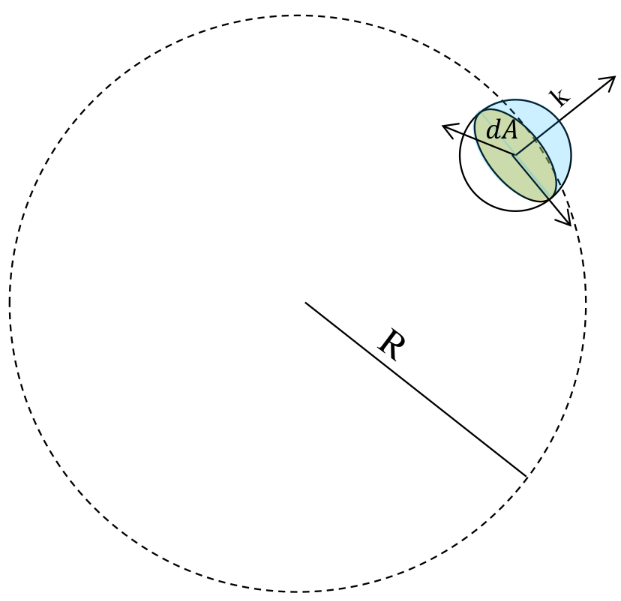
\includegraphics[width=0.25\textwidth]{immagini/emisfera-uscente.png}
\caption{La figura rappresenta un elemento infinitesimo $\ud A$ sulla superficie di una stella. Voglio trovare la radiazione uscente, ovvero quella che attraversa la semisfera uscente che ha come cerchio massimo $\ud A$. Integro in $\ud A$ per ottenere la radiazione uscente da tutta la superficie della stella.}
\label{fig:emisfera-uscente}
\end{figure}

Per ottenere la luminosità totale della sorgente, bisogna integrare su tutta la superficie $4\pi R^2$:
\[
    L_\nu = I_\nu \int_0^{4\pi R^2} \ud A \int_0^{2\pi} \ud \phi \int_0^{\pi/2} \ud \theta \sin{\theta} \cos{\theta}
\]
dove $I_\nu$ è stato portato fuori dagli integrali perché non dipende dagli angoli, essendo la sorgente isotropa. Sviluppando i conti si ottiene un'espressione per la luminosità monocromatica:
\begin{equation}\label{eq:luminosità-monocromatica-intensità}
    L_\nu = 4 \pi R^2 \pi I_\nu
\end{equation}
e integrando su tutte le frequenze si ottiene la luminosità bolometrica:
\begin{equation}\label{eq:luminosità-intensità}
    L = 4 \pi R^2 \pi I
\end{equation}

\subsection{L'equazione del trasporto radiativo e le sue soluzioni}\label{sec:trasporto-radiativo}\label{sec:soluzioni-trasporto-radiativo}

\begin{figure}
\centering
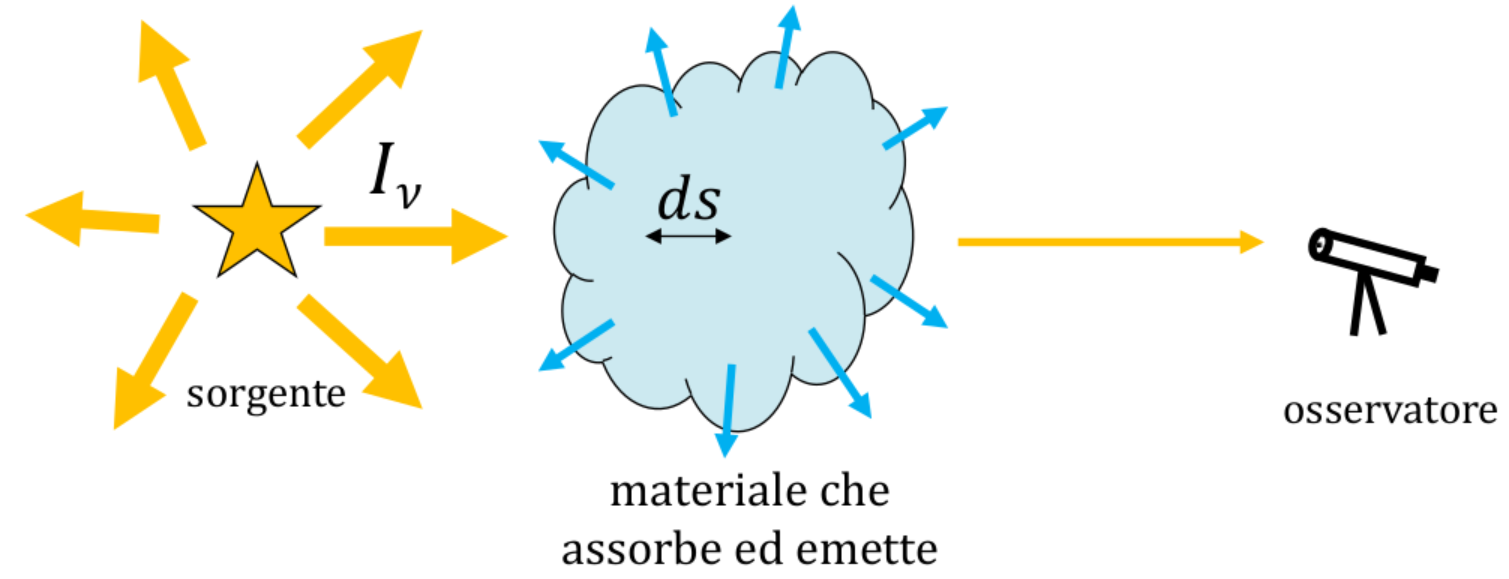
\includegraphics[width=0.7\textwidth]{immagini/trasporto-radiativo.png}
\caption{Equazione del trasporto radiativo. Si studia la variazione di intensità della radiazione emessa dalla sorgente a seguito dell'interazione con il materiale interposto, che avviene attraverso assorbimenti ed emissioni. Lo scattering viene computato nell'assorbimento, poiché l'effetto è quello di deviare la radiazione provocando una diminuzione dell'intensità misurata.}
\label{fig:trasporto-radiativo}
\end{figure}

Come già anticipato nel par.~\ref{sec:intro-trasporto-radiativo}, l'\emph{equazione del trasporto radiativo} descrive la variazione dell'intensità della radiazione a causa dell'interazione tra la radiazione stessa e la materia. Infatti, prima di arrivare all'osservatore, la radiazione attraversa della materia, interagendo attraverso assorbimento ed emissione (fig.~\ref{fig:trasporto-radiativo}). L'equazione si presenta così:
\begin{equation}\label{eq:trasporto-radiativo}
    \ud I_\lambda = - k_\nu \rho I_\nu \ud S + j_\nu \ud S
\end{equation}
dove appaiono i seguenti termini:
\begin{description}
    \item[$\ud I_\nu$] variazione dell'intensità specifica.
    \item[$k_\nu$] coefficiente di assorbimento per unità di massa od opacità ($\si{cm^2.g^{-1}}$). L'opacità ha le dimensioni di una sezione d'urto per unità di massa ed esprime quanta radiazione viene assorbita per unità di massa e per lunghezza attraversata.
    \item[$\rho$] densità di massa del materiale attraversato.
    \item[$I_\nu$] intensità in input.
    \item[$\ud S$] dimensione infinitesima del materiale attraversato.
    \item[$j_\nu$] coefficiente di emissione (\si{erg.s^{-1}.cm^{-3}.Hz^{-1}-sr^{-1}}).
\end{description}

In genere si definisce:
\[
\alpha_\nu = k_\nu \rho
\]
e l'equazione~\eqref{eq:trasporto-radiativo} assume la seguente forma:
\begin{equation}\label{eq:trasporto-radiativo2}
    \frac{\ud I_\nu}{\ud S} = -\alpha_\nu I_nu + j_\nu
\end{equation}

La si può risolvere facilmente in due casi limite. Nel caso si \emph{pura emissione}, corrispondente a $\alpha_\nu = 0$ si ha:
\[
    \frac{\ud I_\nu}{\ud S} = j_nu \qquad I_\nu = I_\nu (0) + \int \ud S j_\nu
\]
In questo caso, l'aumento di densità è pari al coefficiente di emissione integrato lungo la linea di vista.

Nel caso di \emph{puro assorbimento}, corrispondente a $j_\nu = 0$, si ha:
\[
\frac{\ud I_\nu}{\ud S} = -\alpha_\nu I_\nu \quad 
I_\nu (S) = I_\nu (0) e^{-\int \alpha_\nu \ud S}
\]
In questo caso, l'intensità cala come l'esponenziale del coefficiente di assorbimento integrato lungo la linea di vista.

È conveniente introdurre la \emph{profondità ottica} (cfr.~\ref{sec:profondità-ottica}):
\begin{equation}\label{eq:profondità-ottica}
        \tau_\nu = \int k_\nu \rho \ud S
\end{equation}
dove si integra lungo il cammino $\ud S$. La profondità ottica in generale dipende anche dalla frequenza ed è un numero puro. 

È conveniente introdurre anche la \emph{funzione sorgente}:
\begin{equation}\label{eq:funzione-sorgente}
    S_\nu = \frac{j_\nu}{k_\nu \rho} = \frac{j_\nu}{\alpha_\nu}
\end{equation}
Essa esprime il rapporto tra il coefficiente di emissione e quello di assorbimento in termini di $\alpha$ e ha le stesse unità di misura di una intensità specifica.

Con queste due nuove variabili, l'equazione assume una forma particolarmente semplice:
\begin{equation}\label{eq:trasporto-radiativo3}
    \frac{\ud I_\nu}{\ud \tau_\nu} = -I_\nu + S_\nu
\end{equation}
Integriamo l'equazione~\eqref{eq:trasporto-radiativo3}, separando le variabili e riscrivendo l'equazione in una forma più comoda:
\[
    \ud I_\nu = -I_\nu \ud \tau_\nu  + S_\nu \ud \tau_\nu
\]
\[
    \ud I_\nu + I_\nu \ud \tau_\nu  = S_\nu \ud \tau_\nu
\]
\[
    e^{\tau_\nu} (\ud I_nu + I_\nu \ud \tau_\nu)  = e^{\tau_\nu} (S_\nu \ud \tau_\nu)
\]
\[
    d(e^{\tau_\nu} I_\nu) = e^{\tau_\nu} \ud I_\nu + I_\nu e^{\tau_\nu} \ud \tau_\nu
\]
\[
    d(e^{\tau_\nu} I_\nu) = e^{\tau_\nu} S_\nu \ud \tau_\nu
\]
Ricordando che la profondità ottica è un integrale tra $0$ e $S$ e al centro è nullo, come limiti inferiori dell'integrazione scelgo $\tau_{\nu_0} = 0$ e $I_{\nu_0}$, corrispondente all'intensità iniziale, prima dell'interazione con la materia. Suppongo, inoltre, che la funzione sorgente $S_\nu$ non varii con $\tau$, ovvero con la distanza.
\[
    e^{\tau_\nu} I_\nu - I_{\nu_0} = \int_0^{\tau_\nu} e^{\tau_\nu'} S_\nu \ud \tau_\nu' = S_\nu (e^{\tau_\nu} - 1)
\]
Moltiplico ambo i membri per $e^{-\tau_\nu}$
\[
    I_\nu (\tau_\nu) - I_{\nu_0} e^{-\tau_\nu} = S_\nu (1-e^{-\tau_\nu})
\]
da cui si ottiene:
\begin{equation}\label{eq:soluzione-trasporto-radiativo}
    I_\nu = I_{\nu_0} e^{-\tau_\nu} + S_\nu (1- e^{-\tau_\nu})
\end{equation}
Il primo termine è l'intensità iniziale $I_{\nu_0}$(prima dell'interazione con la materia) attenuata da un fattore esponenziale (si ricordi che $\tau \in [1,+\infty]$), mentre il secondo termine \emph{non} dipende dall'intensità iniziale (quella emessa dalla sorgente), ma riguarda solamente il materiale interposto\footnote{Il materiale interposto può anche essere l'atmosfera della stella stessa che si osserva, oppure potrebbe essere l'atmosfera della Terra e così via.}. Trascurando il primo termine, questo secondo termine, che rappresenta l'emissione e l'assorbimento, può anche rappresentare una auto--emissione e un auto--assorbimento nel caso in cui non ci sia una stella "dietro".

\subsection{Trascuro la sorgente di background}\label{sec:trascuro-sorgente-trasporto-radiativo}
Se nell'equazione~\eqref{eq:soluzione-trasporto-radiativo} trascuro la sorgente di background, assume la forma:
\begin{equation}\label{eq:soluzione-no-sorgente-trasporto-radiativo}
    I_\nu = S_\nu (1- e^{-\tau_\nu})
\end{equation}
Questo corrisponde, ad esempio, a osservare il mezzo interposto da una direzione perpendicolare rispetto alla stella, come mostrato in fig.~\ref{fig:trasporto-radiativo-perpendicolare}. Il primo termine, $S_\nu$, rappresenta l'emissione, mentre il secondo termine, $S_\nu e^{-\tau_\nu}$, rappresenta l'auto--assorbimento. Si può studiare l'eq.~\eqref{eq:soluzione-no-sorgente-trasporto-radiativo} considerando due situazioni limite:
\begin{description}
    \item[Regime otticamente spesso] la profondità ottica è molto grande, $\tau_\nu \gg 1$, quindi l'intensità coincide con la funzione sorgente: $I_\nu = S_\nu$
    \item[Regime otticamente sottile] la profondità ottica è molto piccola, $\tau_\nu \ll 1$, quindi l'intensità risulta $I_\nu = S_\nu \tau_\nu$
\end{description}

\begin{figure}
\centering
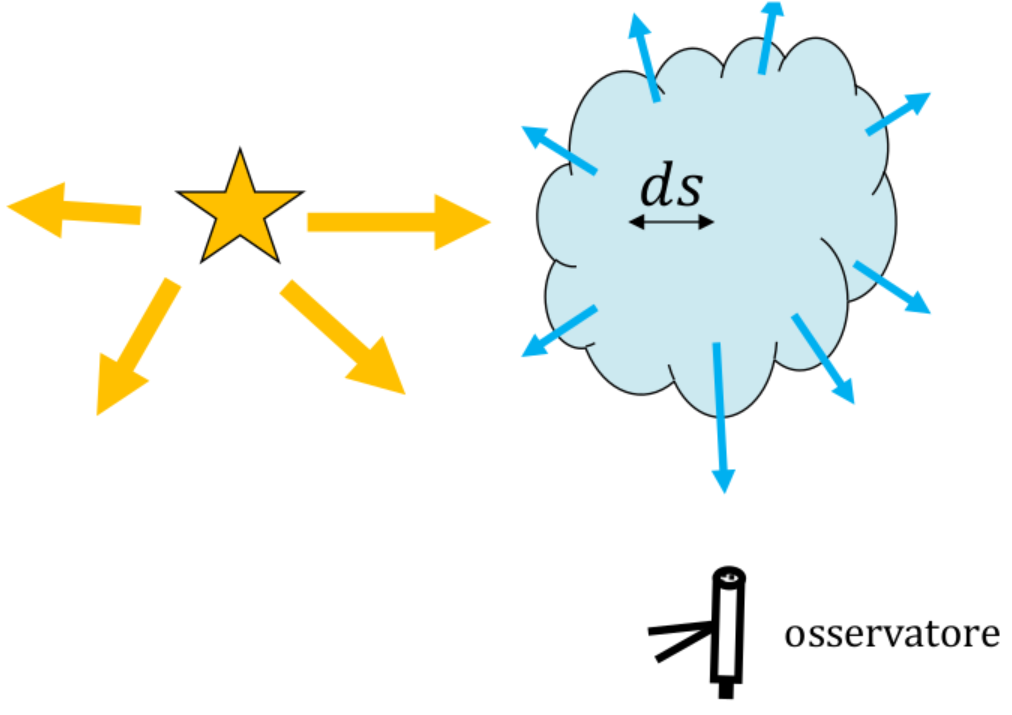
\includegraphics[width=0.3\textwidth]{immagini/trasporto-radiativo-perpendicolare.png}
\caption{Trascuro la sorgente di background nella soluzione dell'equazione del trasporto radiativo.}
\label{fig:trasporto-radiativo-perpendicolare}
\end{figure}

Ci si può chiedere come sia fatta la funzione sorgente $S_\nu$, definita tramite eq.~\eqref{eq:funzione-sorgente}. Essa è diversa a seconda del tipo di radiazione, cioè del processo responsabile del fenomeno di radiazione osservato. Tipicamente i processi di emissione vengono raggruppati in processi termici e processi non termici.
\begin{description}
    \item[Radiazione termica] emessa da un corpo in equilibrio termico (o termodinamico). Ovvero materia e radiazione sono accoppiate, ci sono continui processi di emissione e assorbimento di fotoni e il tasso di assorbimento è uguale al tasso di emissione. Esempi di processi termici sono:
    \begin{itemize}
        \item Radiazione di corpo nero (stelle)
        \item Bremsstrahlung (gas negli ammassi di galassie)
    \end{itemize}
    
    \item[Radiazione non termica] non sono dovuti a processi di emissione e assorbimento, ma, ad esempio, a moto di cariche elettriche oppure a scattering. Esempio sono:
    \begin{itemize}
        \item Sincrotrone (pulsar)
        \item Compton (effetto Sinyaev-Zel'dovich)
    \end{itemize}
\end{description}

\subsection{Radiazione termica}
Se, nell'approssimazione del paragrafo~\ref{sec:trascuro-sorgente-trasporto-radiativo} considero solamente processi termici, ovvero processi dovuti a continue emissioni e assorbimenti, la funzione sorgente coincide con la \emph{funzione di Planck} (eq.~\eqref{eq:corpo-nero}), che verrà introdotta nel prossimo paragrafo:
\[
    S_\nu = B_{BB} (T)
\]
In questo caso, i due regimi di approssimazione si riducono alle seguenti espressioni:
\begin{description}
    \item[regime otticamente spesso ($\tau_\nu \gg 1$)] $I_\nu = B_{BB}$
    \item[regime otticamente sottile ($\tau_\nu \ll 1$)] $I_\nu = B_{BB} \tau_\nu$
\end{description}
È evidente che, se il regime è \emph{otticamente spesso}, la radiazione termica è \emph{radiazione di corpo nero}.

\section{Corpo nero}\label{sec:corpo-nero}

\subsection{Legge di Planck}\label{sec:legge-planck}
Introdotto da Planck alla fine del 1800, un \emph{corpo nero} è un corpo idealizzato in equilibrio termodinamico che assorbe tutta la radiazione incidente ed emette uno spettro che dipende solo dalla temperatura superficiale $T$ del corpo stesso. Il tasso di assorbimento e di emissione è lo stesso e la forma dello spettro del corpo segue la legge di Planck:(fig.~\ref{fig:corpo-nero}):
\begin{equation}\label{eq:corpo-nero}
    B_{BB} (T) = \frac{2 h}{c^2} \frac{\nu^3}{e^{\frac{h \nu}{k_B T}} - 1}
\end{equation}
La planckiana dipende sia dalla \emph{frequenza} che dalla \emph{temperatura} del corpo. Le stelle in prima approssimazione si possono considerare dei corpi neri, come si può osservare da un confronto tra dati sperimentali e curve teoriche in figura~\ref{fig:stelle-corpi-neri}. Guardando come sono fatte le curve a diverse lunghezze d'onda si può inferire la \emph{legge di spostamento di Wien}.

\begin{figure}
\centering
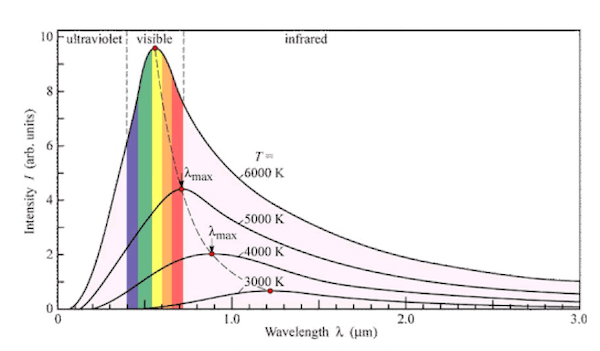
\includegraphics[width=0.5\textwidth]{immagini/corpo-nero.png}
\caption{Legge di Planck. Curve in funzione della frequenza plottate a diverse temperature. I picchi seguono la legge di spostamento di Wien.}
\label{fig:corpo-nero}
\end{figure}

\begin{figure}
\centering
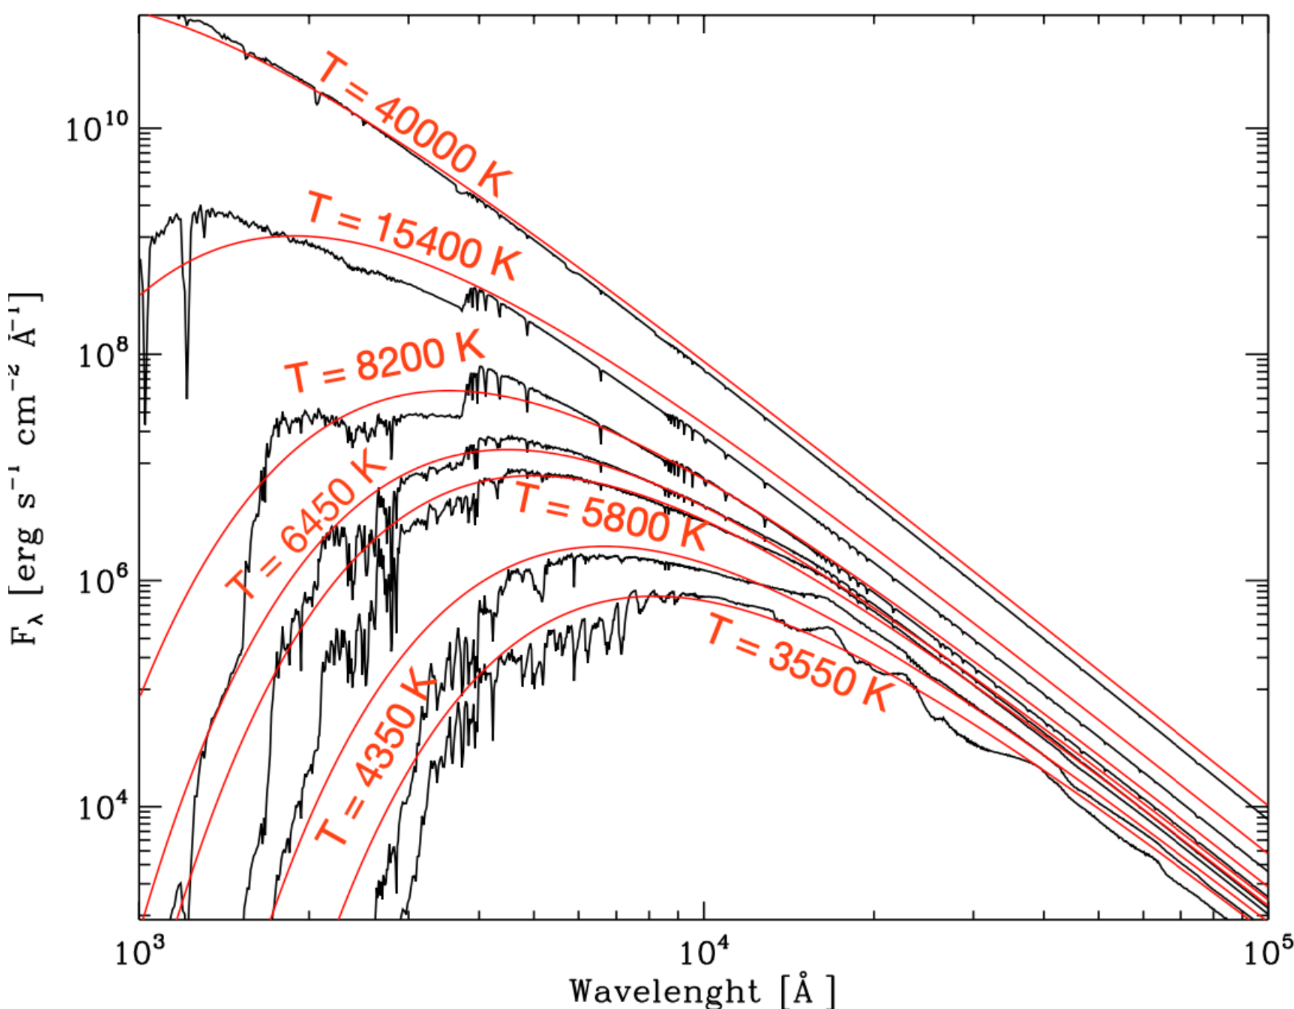
\includegraphics[width=0.4\textwidth]{immagini/stelle-corpi-neri.png}
\caption{Confronto tra i profili teorici di planckiana e dati sperimentali sulle stelle. In prima approssimazione le stelle possono essere trattate come corpi neri.}
\label{fig:stelle-corpi-neri}
\end{figure}

\subsection{Legge di spostamento di Wien}\label{sec:legge-wien}
Più elevata è la temperatura $T$ del corpo, più il picco di emissione si trova a basse lunghezze d'onda, corrispondenti ad alte frequenze (fig.~\ref{fig:corpo-nero}):
\begin{equation}\label{eq:legge-wien}
    T \lambda_\textup{max} = \SI{0.29}{cm.K}
\end{equation}
Da questa legge è immediato capire perché vediamo il nostro sole di colore giallo. Infatti, la sua temperatura sua temperatura superficiale è circa $T \sim \SI{5770}{K}$, da cui una lunghezza d'onda sul picco corrispondente a $\lambda_\textup{max} \sim \SI{0.5}{\mu m}$. Si può esprimere la legge anche in funzione della frequenza, come mostrato in figura~\ref{fig:legge-wien}, ed esprime che più elevata è la temperatura del corpo, più il picco di emissione si trova ad alte frequenze (basse lunghezze d'onda). Quindi, se suppongo che una sorgente che sto osservando sia un corpo nero, effettuando misure a lunghezze d'onda diverse, in base alla frequenza a cui osservo il picco di emissione, posso risalire alla temperatura superficiale della stella. In particolare, una \emph{stella blu} sarà \emph{calda}, mentre una \emph{stella rossa} sarà \emph{fredda}.

\begin{figure}
\centering
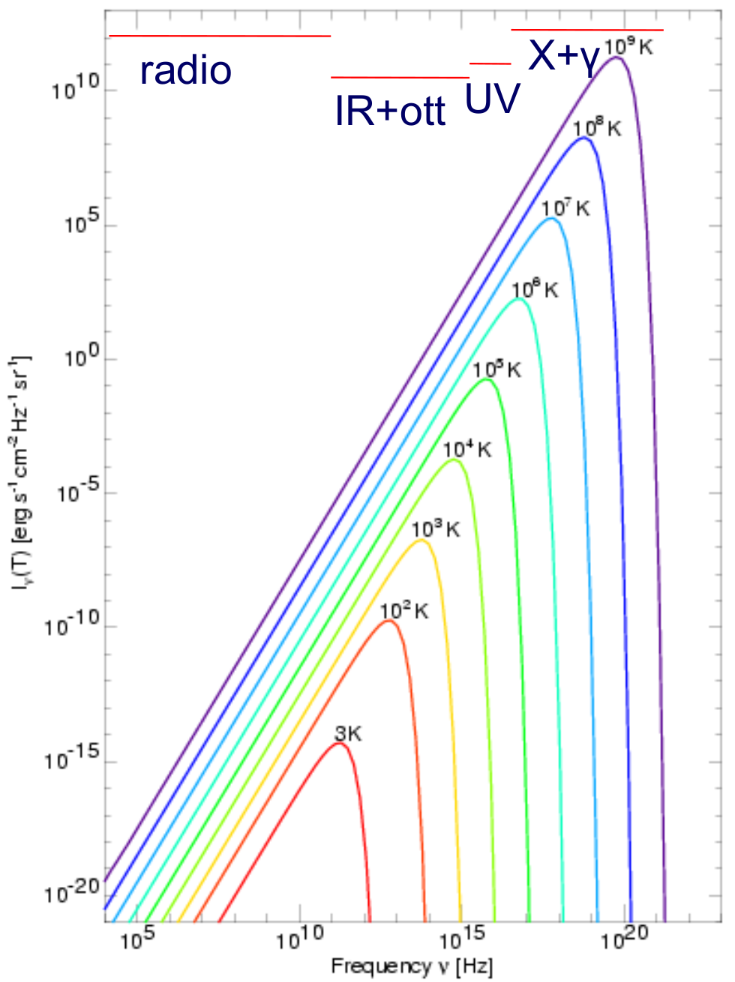
\includegraphics[width=0.3\textwidth]{immagini/legge-wien.png}
\caption{Legge di Wien vista in funzione della frequenza. All'aumentare della temperatura, il picco di emissione si sposta verso frequenze più alte.}
\label{fig:legge-wien}
\end{figure}

\subsection{Legge di Stefan-Boltzmann}\label{sec:legge-stefan-boltzmann}
All'aumentare della temperatura $T$, aumenta anche l'intensità del corpo nero, come si può osservare nell'equazione~\eqref{eq:corpo-nero}. Questo significa che un corpo nero più caldo emetterà più energia al secondo, su tutte le lunghezze d'onda, infatti basta integrare su tutte le lunghezze d'onda, ovvero basta guardare l'area sotto la curva a fissata temperatura nella figura~\ref{fig:corpo-nero}. Ma l'energia totale emessa integrata su tutte le frequenze (par.~\ref{sec:luminosità}) è proprio la luminosità bolometrica $L_\textup{bol}$ del corpo. Questo suggerisce che debba esistere una relazione tra $T$ e $L_\textup{bol}$.

Gli esperimenti di \emph{Josef Stegan} (1879) hanno mostrato che la luminosità bolometrica $L_\textup{bol}$ di un corpo nero di area $A$ alla temperatura $T$, misurata in Kelvin, è data da:
\[
    L_\textup{bol} = A \sigma T^4
\]
dove $\sigma$ è la \emph{costante di Stefan-Boltzmann} e vale:
\[
    \sigma = \SI{5.67e-5}{erg.s^{-1}.cm^{-2}.K^{-4}}
\]
Dunque, data una stella di raggio $R$ e \emph{temperatura superficiale} T:
\begin{equation}\label{eq:stefan-boltzmann}
    L_\textup{bol} = 4 \pi R^2 \sigma T^4
\end{equation}
Inserendo i dati del Sole
\[
    R \sim \SI{7e10}{cm} \qquad T \sim \SI{5770}{K} \qquad \sigma \sim \SI{5.67e-5}{erg.s^{-1}.cm^{-2}.K^{-4}}
\]
si ottiene
\[
    \si{\solarluminosity} \sim \SI{3.8e-33}{erg.s^{-1}}
\]
Si può utilizzare la legge~\eqref{eq:stefan-boltzmann}, ad esempio, per ricavare il raggio di una stella, conoscendone la temperatura superficiale e la luminosità.
\section{Flusso}\label{sec:flusso}
L'intensità (par.~\ref{sec:intensità}) e la luminosità (par.~\ref{sec:luminosità}) sono quantità \emph{intrinseche} della sorgente, ma \emph{non} sono osservabili. Infatti, più una sorgente è lontana da noi, più ci appare debole, ma la sua luminosità non cambia con la distanza, poiché l'energia emessa ogni secondo è sempre la stessa. Ciò che osserviamo è il \emph{flusso}, definito come la luminosità per unità di area: l'energia per unità di tempo per unità di area che arriva sull'apparato di misura. Ovviamente il flusso dipende dalla distanza: diminuisce all'aumentare della distanza dalla sorgente.

Ipotizzando una emissione isotropa, il flusso misurato a una distanza $r$ da una sorgente che emette con una luminosità $L$ è dato da:
\begin{equation}\label{eq:flusso}
    F(r) = \frac{L}{4 \pi r^2}
\end{equation}
Analogamente all'intensità, è possibile definire un \emph{flusso monocromatico}, per unità di frequenza, $F_\nu$, e trovare il flusso totale come:
\[
    F = \int_0^\infty F_\nu \ud \nu
\]
Il flusso e la luminosità delle sorgenti sono spesso espressi in termini di \emph{magnitudini}.
\section{Magnitudine}\label{sec:magnitudine}
\subsection{Magnitudine apparente}\label{sec:magnitudine-apparente}
La \emph{magnitudine apparente} è una misura del flusso ricevuto dallo strumento. È una grandezza introdotta per la prima volta dall'astronomo greco \emph{Ipparco} e varia tra $m=1$, che corrisponde all'oggetto più brillante del cielo, e $m=6$, che corrisponde alle stelle più deboli che si possono osservare a occhio nudo. Si faccia attenzione al fatto che \emph{maggiore è la magnitudine, più debole è la stella}. In particolare, la scala di magnitudini segue la \emph{risposta logaritmica} dell'occhio umano alla luminosità delle stelle che osserviamo sulla volta celeste.

\emph{Norman Robert Pogson} (1856) notò che una magnitudine di $m=6$ corrisponde a una stella $\sim 100$ volte più debole di una con magnitudine $m=1$. Si può quindi osservare che una differenza di $5$ magnitudini corrisponde a un rapporto tra i flussi di $100$:
\[
    m_1=1, \,  m_2=6 \implies F_1 = 100 F_2
\]
\[
    m_2 - m_1 = 5 \implies \frac{F_1}{F_2} = 100 = 100^{\frac{m_2 - m_1}{5}}
\]
Quindi risulta:
\begin{equation}\label{eq:magnitudine-apparente}
    \frac{F_1}{F_2} = 100^{\frac{m_2 - m_1}{5}}
\end{equation}
da ciò segue che una differenza di $1$ magnitudine corrisponde a un rapporto tra i flussi pari a $100^{1 / 5} \sim 2.5$. Quindi, ad esempio, una stella di magnitudine $m=1$ \emph{appare} $2.5$ volte più brillante di una stella di magnitudine $m=2$ e $2.5^5 \sim 100$ volte più brillante di una stella con magnitudine $m=6$. Si parla dunque di magnitudini \emph{apparenti}.

\subsection{Legame tra magnitudine apparente e flusso}\label{sec:relazione-magnitudine-apparente-flusso}
Prendendo il logaritmo ($\log$ sarà il logaritmo in base $10$) di entrambi i membri dell'equazione~\eqref{eq:magnitudine-apparente}, si trova:
\[
    \log\frac{F_1}{F_2} = \frac{m_2 - m_1}{5} \log(100) = \frac{2}{5} (m_2 - m_1) = 0.4 (m_2 - m_1)
\]
Da cui segue:
\begin{equation}\label{eq:relazione-magnitudine-apparente-flusso}
    m_1 - m_2 = -2.5 \log\frac{F_1}{F_2}
\end{equation}
Ovvero, considerando i flussi monocromatici:
\begin{equation}\label{eq:relazione-magnitudine-apparente-flusso-monocromatico}
    m_{1\nu} - m_{2\nu} = -2.5 \log\frac{F_{1\nu}}{F_{2\nu}}
\end{equation}

Misurando il flusso di una sorgente \emph{non} si conosce la sua magnitudine, poiché, come ovvio dall'equazione~\eqref{eq:relazione-magnitudine-apparente-flusso}, è possibile solamente conoscere la magnitudine \emph{rispetto a un'altra sorgente}. È dunque necessario assegnare un valore di magnitudine apparente fisso attraverso un \emph{sistema fotometrico}. Un esempio è il \emph{sistema fotometrico di Vega}, secondo il quale si impone che la stella Vega abbia magnitudine $m=0$ a tutte le frequenze, sicché la relazione tra magnitudine e flusso diventano:
\[
    m_\nu = - 2.5 \log\frac{F_\nu}{F_{0\nu}}
\]
dove $m_\nu$ e $F_\nu$ sono rispettivamente la magnitudine e il flusso della sorgente a una data frequenza $\nu$, mentre $F_{0\nu}$ è il flusso della stella Vega a quella data frequenza. Per farsi un'idea degli ordini di grandezza nel sistema di Vega si faccia riferimento alla tab.~\ref{tab:sistema-fotometrico-vega}.

\begin{table}
\caption{Magnitudini apparenti nel Sistema Fotometrico di Vega. Il Sole, essendo la stella a noi più vicina, è quella che ci \emph{appare} più luminosa, infatti ha la magnitudine assoluta più piccola possibile, ovvero più negativa possibile in questo caso. Il flusso dipende sia dalla luminosità della sorgente sia dalla distanza della sorgente dall'osservatore.}
\label{tab:sistema-fotometrico-vega}
\centering
\begin{tabular}{lS}
\toprule
Oggetto & {Magnitudine apparente} \\
\midrule
Sole         & -26.8 \\
Luna piena   & -12.6 \\
Venere       & -4.7 \\
Giove, Marte & -2.8 \\
Sirio & -1.5 \\
Vega & 0.0 \\
Uranio & 5.5 \\
Più deboli visibili a occhio & 6.0 \\
Nettuno & 7.7 \\
Plutone & 13.0 \\
\bottomrule
\end{tabular}
\end{table}

\subsection{Magnitudine assoluta}\label{sec:magnitudine-assoluta}
Si definisce \emph{magnitudine assoluta} la magnitudine apparente che avrebbe una sorgente se fosse a una distanza di $\SI{10}{parsec}$ ($\SI{1}{pc} = \SI{3.086e18}{cm}$):
\begin{equation}\label{eq:magnitudine-assoluta}
    M = m_{\SI{10}{pc}}
\end{equation}
Essa, a differenza della magnitudine apparente, è legata alla luminosità intrinseca della sorgente ed è possibile ricavare la loro relazione utilizzando l'eq.~\eqref{eq:relazione-magnitudine-apparente-flusso}:
\[
    M_1 - M_2 = m_{1, \SI{10}{pc}} - m_{2, \SI{10}{pc}} = -2.5 \log\frac{F_1 (\SI{10}{pc})}{F_2 (\SI{10}{pc})}
\]
e utilizzando l'equazione~\eqref{eq:flusso} per scrivere:
\[
    \frac{F_1 (\SI{10}{pc})}{F_2 (\SI{10}{pc})} = \frac{L_1}{L_2}
\]
Da ciò segue che:
\begin{equation}\label{eq:magnitudine-assoluta-luminosità}
    M_1 - M_2 = -2.5 \log\frac{L_1}{L_2}
\end{equation}

\subsection{Modulo di distanza}
Conoscendo la magnitudine apparente e la magnitudine assoluta di una sorgente, è possibile stimare la sua distanza attraverso il \emph{modulo di distanza}. Troviamo la relazione tra $m$ e $M$ utilizzando l'equazione~\eqref{eq:relazione-magnitudine-apparente-flusso}:
\[
    m - M = m - m_{\SI{10}{pc}} = -2.5 \log\frac{F(d)}{F(\SI{10}{pc})}
\]
e usando l'equazione~\eqref{eq:flusso} con $r=d$:
\[
    \frac{F(d)}{F(\SI{10}{pc})} = \frac{10^2}{d^2}
\]
Mettendo insieme si trova:
\[
    m - M = -5 \log\frac{10}{d} = -5 + 5 \log d
\]
Da cui l'espressione per il \emph{modulo di distanza}:
\begin{equation}\label{eq:modulo-distanza}
    m - M = -5 + 5 \log(d_{\si{pc}})
\end{equation}
dove con il pedice si è sottolineato che le distanze sono espresse in \emph{parsec}.

Siccome siamo in grado di misurare la distanza del Sole e possiamo misurare la sua magnitudine apparente a varie lunghezze d'onda, utilizzando l'equazione~\eqref{eq:modulo-distanza} è possibile ricavare le magnitudini assolute del sole a varie lunghezze d'onda, ad esempio si ha (B, V e K sono tre differenti filtri fotometrici):
\[
    M_\ensuremath{\textup{bol}\odot} = 4.75 \quad M_\ensuremath{\textup{B}\odot} = 5.48 \quad M_\ensuremath{\textup{V}\odot} = 4.83 \quad M_\ensuremath{\textup{K}\odot} = 3.31
\]
Queste sono utilizzate come riferimento per esprimere la luminosità e la magnitudine assoluta per ogni altra sorgente. Infatti, richiamando l'equazione~\eqref{eq:magnitudine-assoluta-luminosità} e imponendo $M_2 = \si{\solarmass}$ e $L_2 = \si{\solarluminosity}$, si ottiene
\begin{equation}\label{eq:magnitudine-assoluta-luminosità-sole}
    M_1 - \si{\solarmass} = -2.5 \log\frac{L_1}{\si{\solarluminosity}}
\end{equation}
\section{Colore}\label{sec:colore}
\subsection{Definizione di colore}
L'\emph{indice di colore} è la differenza tra le magnitudini misurate in due diverse bande fotometriche (\emph{filtri}). In particolare, le immagini vengono acquisite attraverso filtri che selezionano solamente alcune lunghezze d'onda. Ciascun filtro ha la propria curva di trasmissione, centrata su una data lunghezza d'onda. D'altra parte, ciascuna sorgente ha il proprio spettro di emissione. Quindi, i diversi filtri selezionano solo una frazione dello spettro della sorgente, quella inclusa sotto la loro curva di trasmissione (fig.~\ref{fig:filtri-fotometrici}). Ne conviene che il flusso misurato durante l'osservazione in un dato filtro dipende sia dal filtro che dallo spettro della sorgente.

\begin{figure}
\centering
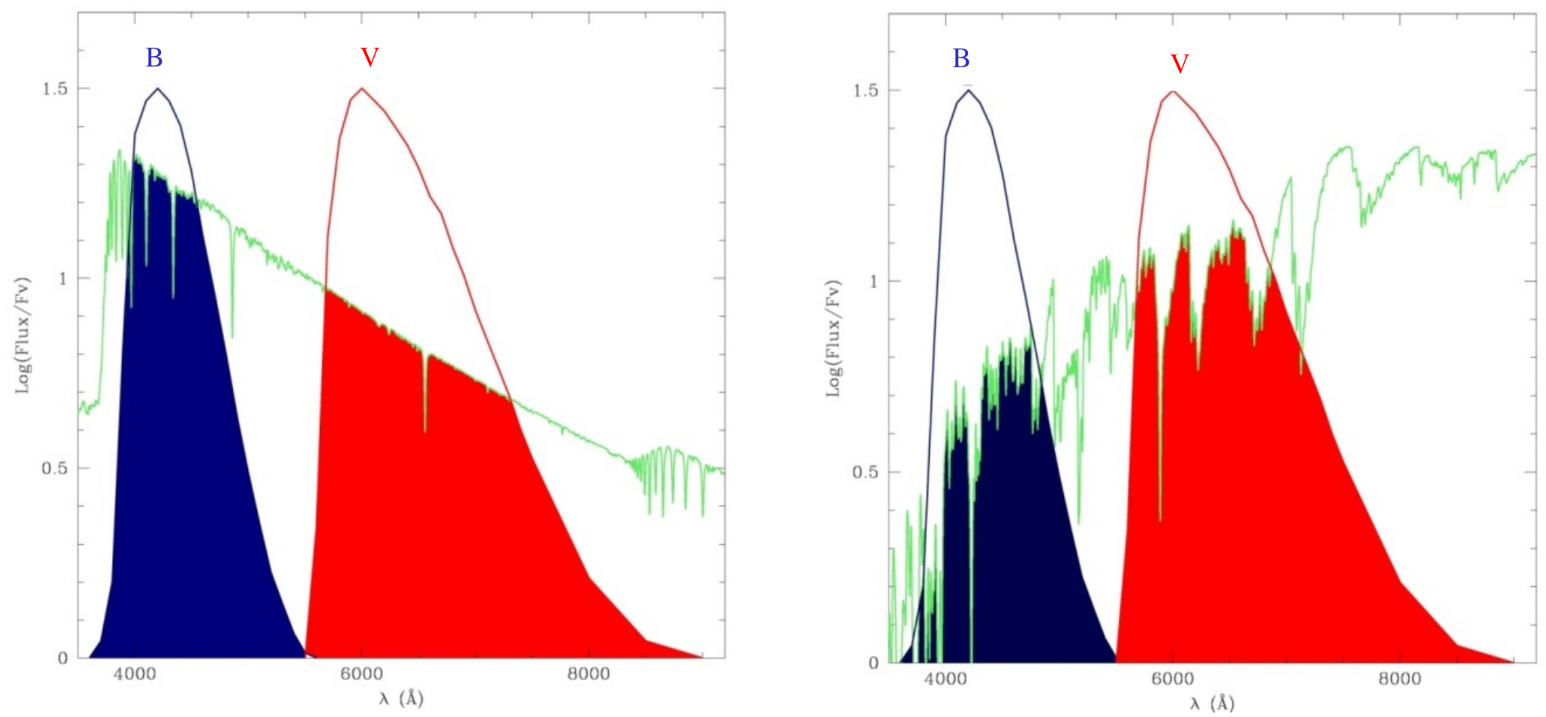
\includegraphics[width=0.7\textwidth]{immagini/filtri-fotometrici.png}
\caption{Osservazione di due spettri diversi con due filtri, uno blu (B) e uno rosso (V). In verde sono rappresentati gli spettri analizzati e le curve in blu e rosso sono rispettivamente le curve di trasmissione del filtro blu e rosso. Le zone evidenziate rappresentano il flusso misurato. Si nota che a sinistra vale $F_B > F_V$ mentre a destra $F_B < F_V$. Ciò evidenzia come il flusso misurato dipende sia dallo spettro della sorgente che dal filtro utilizzato.}
\label{fig:filtri-fotometrici}
\end{figure}

Ricordando l'equazione~\eqref{eq:relazione-magnitudine-apparente-flusso}, si può scrivere:
\[
    m_B = -2.5 \log F_B + \textup{const}
\]
\[
    m_V = -2.5 \log F_V + \textup{const}
\]
dove $m_B$ e $m_V$\footnote{il pedice V sta per \emph{vermillion}.} sono le magnitudini apparenti rispettivamente in filtro blu e filtro rosso (analogo per i flussi misurati $F_B$ e $F_V$). Si definisce \emph{colore} la differenza tra la magnitudine misurata col filtro più blu e la magnitudine misurata col filtro più rosso:
\begin{equation}\label{eq:colore}
    m_B - m_V \equiv B-V
\end{equation}
Il colore, dunque, è un numero puro, e in tab.~\ref{tab:colore} sono presenti le relazioni tra il colore, la magnitudine apparente e il flusso in filtro blu e rosso. 

\begin{table}
\caption{Relazione tra colore, magnitudine apparente e flusso.}
\label{tab:colore}
\centering
\begin{tabular}{lll}
\toprule
Colore & Magnitudine apparente & Flusso \\
\midrule
$<0$ & $m_B < m_V$ & $F_B > F_V$ \\
$=0$ & $m_B = m_V$ & $F_B = F_V$ \\
$>0$ & $m_B > m_V$ & $F_B < F_V$ \\
\bottomrule
\end{tabular}
\end{table}

Ovviamente, cambiando i filtri, cambia anche la denominazione del colore. Si tenga inoltre in considerazione che il colore \emph{non} dipende dalla distanza, infatti sto considerando la stessa stella, pertanto nella~\eqref{eq:relazione-magnitudine-apparente-flusso} dovremo considerare la stessa distanza per il flusso~\eqref{eq:flusso}. Da ciò è immediato che la differenza tra le magnitudini apparenti e le magnitudini assolute è uguale:
\begin{equation}\label{eq:differenza-magnitudini-apparente-assoluta}
    m_B-m_V = M_B-M_V
\end{equation}

\subsection{Colore e temperatura}
Ci si può chiedere quale sia la ragione fisica alla base del diverso colore delle stelle. Ripensando all'esempio in fig.~\ref{fig:filtri-fotometrici} è evidente che una stella è tanto più blu quanto maggiore è il flusso misurato a basse lunghezze d'onda. Dunque, in definitiva, la ragione fisica del diverso colore è la stessa del diverso spettro. Come introdotto nel par.~\ref{sec:legge-planck} ed evidenziato in fig.~\ref{fig:stelle-corpi-neri}, le stelle in prima approssimazione sono dei corpi neri, dunque lo spettro è definito dall'equazione di Planck~\eqref{eq:corpo-nero}. Utilizzando un particolare filtro, si sta fissando la lunghezza d'onda (o frequenza) di picco a cui lavora tale filtro, dunque lo spettro osservato di una stella dipenderà solamente dalla sua \emph{temperatura superficiale}. Ricordando la relazione tra intensità e luminosità monocromatica espressa dall'eq.~\eqref{eq:luminosità-monocromatica-intensità} e imponendo per una stella $I_\nu = B_\nu (T)$ si ottiene:
\[
    L_\nu = 4 {\pi}^2 R^2 B_\nu (T)
\]
da cui, attraverso la relazione~\eqref{eq:magnitudine-assoluta-luminosità}, usando~\eqref{eq:differenza-magnitudini-apparente-assoluta}, si ottiene
\[
    m_{\lambda 1} - m_{\lambda 2} = M_{\lambda 1} - M_{\lambda 2} = -2.5 \log\frac{L_{\lambda 1}}{L_{\lambda 2}} = -2.5 \log\frac{B_{\lambda 1}(T)}{B_{\lambda 2}(T)}
\]
da cui si può inferire che, nel limite di validità dell'approssimazione della stella come corpo nero, il colore dipende solamente dalla temperatura.

Per riassumere, più bassa è la temperatura superficiale, più rossa è la stella, che equivale a un grande $(B-V)$, mentre più alta è la temperatura superficiale, maggiore è il flusso a basse $\lambda$ (cfr. fig.~\ref{fig:corpo-nero}) e più blu è la stella, che equivale a un piccolo $(B-V)$.

\subsection{Estinzione (reddening)}\label{sec:reddening}
In generale, a causa dei processi d'interazione tra radiazione e materia nel cammino tra la sorgente e l'osservatore, una stella tende ad apparire \emph{più debole} e \emph{più rossa} di come non sia veramente, questo fenomeno prende il nome di \emph{estinzione} (o arrossamento). È possibile esprimere tale fenomeno analiticamente, introducendo un parametro di correzione alla magnitudine "intrinseca", ovvero quella che vedremmo se non ci fosse l'interazione con il mezzo interstellare.
\begin{equation}\label{eq:estinzione}
    m_\lambda = m_{\lambda 0} + A_\lambda
\end{equation}
dove $m_\lambda$ è la magnitudine osservata, $m_{\lambda 0}$ quella intrinseca e $A_\lambda$ prende il nome di \emph{parametro di estinzione}. Esso è relativo alla direzione in cui viene osservata la stella e dipende fortemente dalla lunghezza d'onda, in particolare $A_\lambda$ cresce al diminuire di $\lambda$. La dipendenza di $A_\lambda$ da $\lambda$, detta \emph{legge di estinzione}, è tuttavia scarsamente nota: dipende infatti dalle proprietà del mezzo interstellare lungo la linea di vista, quindi sicuramente cambia al variare della linea di vista, e cambia al variare della galassia che si sta considerando.

È presente una legge di estinzione standard per la Via Lattea, derivata da \emph{Cardelli} (1989), tuttavia probabilmente non è valida ovunque nella nostra galassia e non è chiaro se debba valere anche per altre galassie. L'unica cosa chiara è che l'effetto dell'estinzione cresce al diminuire delle lunghezze d'onda.

Per spiegare l'effetto del \emph{reddening} consideriamo due filtri particolari, un B e un V, e utilizziamo l'equazione~\eqref{eq:estinzione} in combinazione con la~\eqref{eq:colore}. Possiamo scrivere:
\[
    m_\lambda - m_{\lambda 0} = A_\lambda
\]
\[
    B - B_0 = A_B \qquad V - V_0 = A_V
\]
e sottraendo membro a membro:
\[
    B_0 - V_0 \equiv (B-V)_0 = (B-V) - (A_B - A_V)
\]
Il primo termine, $(B-V)_0$, rappresenta il \emph{colore intrinseco}, $(B-V)$ rappresenta il \emph{colore osservato}, mentre l'ultimo termine, $(A_B-A_V) \equiv \EBV$ rappresenta il \emph{reddening}, ovvero l'eccesso di colore. Partendo dal reddening dei filtri B-V si può indicare l'effetto per dei filtri qualunque, moltiplicando per un opportuno fattore correttivo $R_\lambda$:
\begin{equation}\label{eq:reddening}
    m_\lambda = m_{\lambda 0} + A_\lambda = m_{\lambda 0} + R_\lambda \EBV
\end{equation}

\subsection{Modulo di distanza e reddening}
Si faccia attenzione al fatto che la magnitudine apparente che compare nell'espressione del modulo di distanza~\eqref{eq:modulo-distanza} è quella \emph{vera}, ovvero de--arrossata. Talvolta, tuttavia, in letteratura si trova il modulo di distanza \emph{osservato}, ad esempio, in banda V. In questo caso, per trovare la distanza, è necessario de--arrossare:
\[
    (m - M)_V = -5 + 5 \log(d_{\si{pc}}) + 3.12 \, \EBV
\]
Si faccia attenzione anche a un'ultima cosa: la magnitudine assoluta, per definizione, è sempre quella vera. Non ha senso parlare di magnitudine assoluta arrossata.


\chapterimage{cover/head4.png}
\chapter{Struttura stellare}
\section{Modelli stellari}\label{sec:modelli-stellari}
Cos'è una stella? Una \emph{stella} è una sfera auto-gravitante di gas in equilibrio idrostatico, ossia in cui la forza di pressione del gas eguaglia la forza di gravità. I parametri principali con cui si descrive una stella sono la sua \emph{massa} $M$ e la sua \emph{composizione chimica}; solitamente quest'ultima viene espressa con la convenzione riportata di seguito:
\begin{description}\label{tab:composizione-chimica}
    \item[X] Frazione in massa dell'\emph{idrogeno}.
    \item[Y] Frazione in massa dell'\emph{elio}.
    \item[Z] Frazione in massa degli elementi più pesanti dell'elio, ovvero dei \emph{metalli}.
\end{description}
Ovviamente si ha per costruzione che $X + Y + Z = 1$. La maggior parte della frazione in massa di una stella è costituita da idrogeno, anche se la loro composizione varia nel corso della loro vita. Per il Sole, ad esempio, si ha:
\[
    X=0.70 \qquad Y=0.28 \qquad Z=0.02
\]

Una stella è caratterizzata da tre regioni principali:
\begin{itemize}
    \item \textbf{Nucleo:} in questa zona, che è la più interna, viene prodotta l'energia.
    \item \textbf{Inviluppo:} in questa zona l'energia è trasportata in superficie; ci sono zone radiative e convettive (a seconda di come avviene il trasporto di energia verso la superficie della stella).
    \item \textbf{Atmosfera:} è a sua volta suddivisa in tre zone:
    \begin{itemize}
        \item \textbf{Fotosfera:} si tratta dello strato responsabile per la maggior emissione di luce. Sotto la fotosfera la stella è opaca, cioè non emette praticamente nulla.
        \item \textbf{Cromosfera:} suesto strato è quello che vediamo durante un'eclissi.
        \item \textbf{Corona:} è lo strato più esterno della stella, anche questo può essere visto durante un'eclissi.
    \end{itemize}
\end{itemize}

Lo studio di una stella parte dallo studio delle sue caratteristiche osservabili, che sono la magnitudine e il colore che vengono dall'atmosfera; per interpretare le misurazioni e inferire la sua struttura interna, è necessario un \emph{modello stellare}. Esso prenderà in input la massa e la composizione chimica della stella che stiamo prendendo in considerazione e da queste sarà in grado di darci in output la luminosità e la temperatura superficiale, quindi possiamo schematizzarlo come segue:
\begin{center}
    \begin{tikzpicture} [
            blu/.style={rectangle, draw=blue!60, fill=blue!5, very thick, minimum size=5mm},
            red/.style={rectangle, draw=red!60, fill=red!5, very thick, minimum size=5mm},
            green/.style={rectangle, draw=green!60, fill=green!5, very thick, minimum size=5mm},]
        \node[red](1){\footnotesize{Massa, X, Y , Z}};
        \node[blu](2)[right=of 1]{\footnotesize{Modello Stellare}};
        \node[green](3)[right=of 2]{\footnotesize{$L, T_e$}};
        \draw[->] (1.east) -- (2.west);
        \draw[->] (2.east) -- (3.west);
    \end{tikzpicture}
\end{center}

Tuttavia, massa e composizione chimica \emph{non} sono direttamente osservabili, quindi, dovrò tenere conto di tutti i fenomeni fisici visti in precedenza e ricondurmi a tali grandezze attraverso la \emph{magnitudine} e il \emph{colore} per confrontare teoria e dati sperimentali. 

Di seguito sono esposte le sette equazioni necessarie per un modello stellare esaustivo:
\begin{enumerate}
    \item \emph{Equilibrio idrostatico}:
    \[
    \dfrac{\ud P(r)}{\ud r} = -\dfrac{G M(r)}{r^2} \rho(r)
    \]
    \item \emph{Continuità di massa}:
    \[
    \dfrac{\ud M(r)}{\ud r} = 4 \pi r^2 \rho(r)
    \]
    \item \emph{Equazione di stato}:
    \[
    P = \dfrac{aT^4}{3} + \dfrac{k \rho T}{\mu_i H} + 
    \begin{dcases} 
    \frac{k \rho T}{\mu_e H} \\ 
    k_1 \rho^{5/3} \\ 
    k_2 \rho^{4/3}
    \end{dcases}
    \]
    \item \emph{Bilancio energetico}:
    \[
    \dfrac{\ud L(r)}{\ud r} = 4 \pi r^2 \rho(r) \epsilon
    \]
    \item \emph{Gradiente radiativo e criterio di Schwarzschild}:
    \[
    \dfrac{\ud T}{\ud r}\Big|_\textup{rad} = - \dfrac{3 \kappa \rho}{4 \pi r^2} \dfrac{L(r)}{4 a c T^3}
    \]
    \[
    \text{se} \quad \abs*{\dfrac{\ud T}{\ud r}}_\textup{rad} > \abs*{\dfrac{\ud T}{\ud r}}_\textup{ad} \implies \text{c'è convezione.}
    \]
    \item \emph{Opacità}:
    \[
    \kappa = \kappa(\rho, T) 
    \begin{dcases} 
    \kappa_{BF} \propto 10^{25} Z(1 + X) \frac{\rho}{T^{3.5}} \\ 
    \kappa_{FF} \propto 10^{22} (X+Y)(1+X) \frac{\rho}{T^{3.5}} \\ 
    \kappa_{E} \propto 0.2 (1+X) \\ 
    \end{dcases}
    \]
    \item \emph{Produzione di energia tramite reazioni termonucleari}:
    \[
    \epsilon = \epsilon(X, \rho, T) 
    \begin{dcases} \epsilon_{PP} = \epsilon_1 \rho X^2 T_6^\alpha \quad \alpha \in [3.5 - 6] \\ 
    \epsilon_{CN} = \epsilon_2 \rho X X_{CN} T_6^\beta \quad \beta \in [13 - 20] \\ 
    \epsilon_{3\alpha} = \epsilon_3 \rho^2 Y^3 T_8^\gamma \quad \gamma \in [20 - 30] \\
    \end{dcases}
    \]
\end{enumerate}
\section{Equilibrio idrostatico}\label{sec:equilibrio-idrostatico}
L'equazione dell'\emph{equilibrio idrostatico} esprime la condizione per cui la pressione interna del gas che compone la stella è in equilibrio con la forza di gravità data dalla massa della stella stessa. Si può riassumere nella seguente maniera:
\begin{equation}\label{eq:equilibrio-idrostatico}
    \dfrac{\ud P(r)}{\ud r} = -\dfrac{G M(r)}{r^2} \rho(r)
\end{equation}

\begin{figure}
\centering
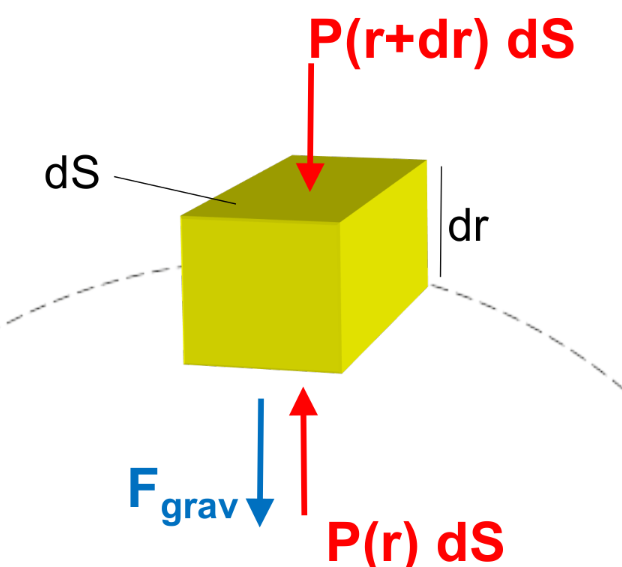
\includegraphics[width=0.3\textwidth]{immagini/equilibrio-idrostatico.png}
\caption{Volumetto infinitesimo a distanza $r$ dal centro della stella. Sulla faccia superiore agisce la pressione che spinge verso il centro. Sulla faccia inferiore agiscono la pressione, verso l'esterno, e la forza di gravità, verso il centro.}
\label{fig:equilibrio-idrostatico}
\end{figure}

Per ricavare tale equazione immaginiamo di dividere la stella in gusci sferici concentrici a temperatura e densità costanti; ognuno di questi è caratterizzato da un valore di densità e di temperatura decrescenti all'aumentare dalla distanza dal centro. Consideriamo un volume infinitesimo di stella a una distanza $r$ dal centro; come mostrato in fig.~\ref{fig:equilibrio-idrostatico}, sulla faccia esterna del volumetto agisce una forza di pressione verso l'interno, mentre sulla faccia interna agisce una forza di pressione verso l'esterno e la forza gravitazionale, verso l'interno. Per imporre la condizione di equilibrio è sufficiente scrivere le espressioni per la forza di pressione $F_p$ e per la forza di gravità $F_g$. Si tenga conto che stiamo considerando l'asse radiale rivolto verso il centro, sicché le forze che agiscono verso l'esterno avranno segno negativo.
\[
    F_p = P(r+\ud r) \ud S - P(r) \ud S = \frac{\ud P(r)}{\ud r} \ud r \ud S
\]
\[
    F_g = \frac{GM(r)}{r^2} \rho(r) \ud r \ud S
\]
dove $M(r)$ rappresenta la massa contenuta all'interno del guscio di raggio $r$, il termine $GM(r) / r^2$ rappresenta l'accelerazione locale di gravità e il termine $\rho(r) \ud r \ud S$ rappresenta la massa del volumetto preso in considerazione. Imponendo l'equilibrio si trova:
\[
    F_p + F_g = 0 \iff \frac{\ud P(r)}{\ud r} \ud r \ud S+ \frac{GM(r)}{r^2} \rho(r) \ud r \ud S = 0
\]
da cui segue immediatamente l'eq.~\eqref{eq:equilibrio-idrostatico}. Quindi, in ogni guscio sferico della stella a fissata distanza $r$ dal centro, la gravità è bilanciata dalla pressione interna del gas. In particolare, è più corretto affermare che la gravità è bilanciata dal \emph{gradiente di pressione}, ovvero dalla variazione di $P$ col raggio. La pressione deve decrescere all'aumentare del raggio, sicché la pressione nel centro della stella è maggiore della pressione vicino alla sua superficie. 

Quando $F_g$ e $F_p$ \emph{non} sono bilanciate, la stella si contrae per $F_g > F_p$ o espande per $F_g < F_p$ in un \emph{tempo caratteristico} pari a:
\[
    T_d = \sqrt{\frac{2r}{g}} = \sqrt{\frac{2r^3}{GM}}
\]

Ci potremmo chiedere quanto ci vorrebbe per una stella come il Sole a collassare se la pressione scomparisse improvvisamente: utilizzando l'equazione sopra otterremmo un tempo di circa 38 minuti.
\input{capitoli/stelle/continuità-massa.tex}
\section{Equazione di stato}\label{sec:equazione-stato}
Guardando le equazioni~\eqref{eq:equilibrio-idrostatico} e~\eqref{eq:continuità-massa}, queste sono 2 equazioni in 3 incognite: $P(r)$, $M(r)$ e $\rho(r)$. Una relazione tra $P$ e $\rho$ è stabilita dall'\emph{equazione di stato}:
\begin{equation}\label{eq:equazione-stato}
    P = \dfrac{aT^4}{3} + \dfrac{k \rho T}{\mu_i H} + 
    \begin{cases} 
    \dfrac{k \rho T}{\mu_e H} \\ 
    k_1 \rho^{5/3} \\ 
    k_2 \rho^{4/3}
    \end{cases}
\end{equation}

Un primo aspetto da considerare è che al pressione nell'interno delle stelle è dovuta a due contributi, ossia la \emph{pressione di radiazione} e \emph{la pressione del gas}:
\[
P = P_\textup{rad} + P_\textup{gas}
\]
\subsection{Pressione di radiazione}
I fotoni esercitano una pressione perché a ogni fotone di energia $E$ è associato un impulso $p = E / c$. Una stella si può approssimare come un corpo nero, dunque è possibile calcolare la pressione di radiazione attraverso la legge di Planck~\eqref{eq:corpo-nero}.
\[
P_\textup{rad} = \frac{4\pi}{3c}\int_0^\infty B_\nu(T) \ud \nu = \frac{1}{3} a T^4
\]
dove $a$ è una costante pari a $a = 4 \sigma / c = \SI{7.6e-15}{erg.cm^{-3}.K^{-4}}$, in cui $\sigma$ è la costante di Stefan-Boltzmann. Accontentiamoci del risultato senza ulteriori specificazioni sui dettagli del conto, quindi si ha:
\begin{equation}\label{eq:pressione-radiazione}
    P_\textup{rad} = \frac{1}{3} a T^4
\end{equation}
Si noti come la pressione di radiazione \emph{non} dipenda dalla densità della stella e invece dipenda fortemente dalla temperatura.

\subsection{Pressione del gas ideale}\label{sec:gas-perfetto}
A causa delle temperature elevate negli interni stellari, gli atomi sono ionizzati e possiamo pensare al gas stellare come a un \emph{plasma di ioni e elettroni}. Quindi, nella maggior parte dei casi, anche a densità e pressioni elevate, il gas stellare può essere trattato come un \emph{gas ideale}, in cui si trascurano le interazioni tra le particelle del gas e la distribuzione delle velocità è rappresentata dalla distribuzione di Maxwell. La densità del gas, in questo caso, dipende sia dalla pressione che dalla temperatura e viceversa, quindi si avrà una pressione che è funzione di densità e temperatura: 
\[
P = P (\rho, T)
\]
Per un gas ideale, inoltre, vale la nota legge:
\begin{equation}\label{eq:standard-gas-ideale}
    PV = N \kb T
\end{equation}
Utilizzando l'equazione~\eqref{eq:standard-gas-ideale} e definendo $\langle m \rangle \equiv M / N$ la massa media delle particelle del gas, e $\rho \equiv M / V$ la densità, si ottiene:
\[
P = \frac{N}{V} \kb T = \frac{N}{M} \frac{M}{V} \kb T = \frac{\kb \rho T}{\langle m \rangle}
\]
In più la massa media delle particelle del gas può essere scritta anche come $\langle m \rangle = \mu H$, dove $\mu$ è il \emph{peso molecolare medio} e $H$ rappresenta la massa di un nucleo di idrogeno, ovvero la massa del protone ($H = m_P = \SI{1.6e-24}{g}$). Mettendo tutto insieme si ottiene l'equazione di stato per un gas ideale:
\begin{equation}\label{eq:gas-ideale}
    P_\textup{gas} = \frac{\kb \rho T}{\mu H}
\end{equation}
Vediamo che la costante di proporzionalità $\rho / \mu H$ dipende dalla massa del gas, che a sua volta dipende dalla composizione chimica.

La caratteristica più importante di questa equazione è la cosiddetta \emph{termo-regolazione}: se $T$ cresce $P$ cresce, ma se $P$ cresce la stella si espande, ma se la stella si espande la temperatura diminuisce, quindi si ha continuamente un bilancio fra pressione e temperatura. Si faccia tuttavia attenzione al fatto che non tutti i gas si comportano come un gas ideale (par.~\ref{sec:degenerazione}).

\subsection{Peso molecolare medio}\label{sec:peso-molecolare}
Arrivati a questo punto ci interessa legare il \emph{peso molecolare medio} $\mu$ alla composizione chimica del gas, introdotta nel par.~\ref{sec:modelli-stellari}. Come già ricordato, $\mu$ rappresenta la media delle masse delle particelle che compongono il gas, espressa in termini della massa del protone $H$:
\begin{equation}\label{eq:peso-molecolare-medio-definizione}
    \mu = \frac{\langle m \rangle}{H}
\end{equation}
D'altra parte, conoscendo la massa totale del gas $M_\textup{tot}$ e il numero totale di particelle libere $N_\textup{free}$, si può calcolare la massa media delle particelle come:
\begin{equation}\label{eq:massa-media-particelle}
    \langle m \rangle = \frac{M_\textup{tot}}{N_\textup{free}}
\end{equation}
Si faccia molta attenzione al fatto che $N_\textup{free}$ rappresenta le particelle libere, dunque, in un gas ionizzato è pari alla somma del numero degli \emph{ioni} e degli \emph{elettroni}. Esso dipende da:
\begin{itemize}
    \item la \emph{composizione chimica del gas}, ovvero da $X$, $Y$ e $Z$ (vedi par.~\ref{sec:modelli-stellari}).
    \item lo \emph{stato di ionizzazione} del gas. In particolare:
    \begin{itemize}
        \item ogni atomo \emph{neutro} contribuisce con 1 particella, ovvero l'atomo stesso.
        \item ogni atomo \emph{totalmente ionizzato} contribuisce con $1+Z_a$ particelle, ovvero il nucleo e $Z_a$ elettroni ($Z_a$ è il numero atomico).
        \item ogni atomo \emph{parzialmente ionizzato} contribuisce con un numero compreso fra $1$ e $1+Z_a$ di particelle.
    \end{itemize}
\end{itemize}
Si faccia nuovamente attenzione a due dettagli. Innanzi tutto, stiamo dividendo il gas studiato in tre parti: l'idrogeno, la cui abbondanza in massa è espressa da $X$, l'elio, la cui abbondanza è espressa da $Y$ e gli elementi più pesanti, la cui abbondanza è $Z$. Dunque, non stiamo distinguendo tra gli elementi più pensanti dell'elio, bensì li stiamo accorpando tutti in una stessa famiglia. Questo è lecito poiché le loro abbondanze sono ridotte in confronto ai primi due elementi della tavola periodica. Inoltre, $Z_a$ rappresenta il grado di ionizzazione del gas per un gas totalmente ionizzato, che coincide dunque con il numero di protoni del gas.

Tenendo a mente che stiamo distinguendo solamente tre specie di elementi (idrogeno, elio e più pesanti), indicizziamo la specie con l'indice $j$, con $j = 1, \, 2, \, 3$; a costo di essere ridondanti, ribadiamo che $j=1$ si riferisce all'idrogeno, $j=2$ all'elio e $j=3$ a tutti gli altri elementi. A questo punto possiamo calcolare il numero di atomi della specie $j$-esima:
\begin{equation}\label{eq:numero-atomi-specie}
    N_j = \frac{M_{\textup{tot}, j}}{m_{\textup{atomo}, j}} \simeq \frac{M_{\textup{tot}, j}}{A_j H}
\end{equation}
dove $A_j$ è il \emph{numero di massa}, ovvero il numero di nucleoni, pari alla somma dei protoni e dei neutroni. In particolare, se consideriamo l'isotopo più comune dell'idrogeno, il prozio, il suo nucleo è composto solamente da un protone, per cui $A_1 = 1$. Considerando l'elio $4$, il suo nucleo è composto da $2$ protoni e $2$ neutroni, pertanto $A_2 = 4$. Invece per gli elementi più pesanti possiamo considerare che i più stabili in genere hanno un numero di protoni circa uguale al numero di elettroni (come abbiamo visto nel corso di Fisica Nucleare questo non è propriamente vero perché la repulsione coulombiana sfavorisce l'aumento dei protoni, quindi al crescere di A avremo in genere un maggior numero di neutroni; ciò nonostante la variazione non è troppo significativa, quindi possiamo assumere che il numero di protoni e quello di neutroni in genere sia lo stesso). Se consideriamo un gas \emph{totalmente ionizzato}, gli elementi più pesanti avranno $\sim Z_a$ particelle libere (con $Z_a$ il loro numero atomico) e avremo $A_3 \sim 2 Z_a$.

Inoltre possiamo scrivere l'abbondanza in massa della specie $j$-esima utilizzando la definizione stessa, ossia: 
\begin{equation}\label{eq:definizione-abbondanza}
    X_j = \frac{M_{\textup{tot}, j}}{M_\textup{tot}}
\end{equation}
dove $X_1 = X$, $X_2 = Y$ e $X_3 = Z$, come più volte ricordato. Mettendo insieme le equazioni~\eqref{eq:numero-atomi-specie} e~\eqref{eq:definizione-abbondanza} si trova:
\begin{equation}\label{eq:numero-atomi-specie2}
    N_j =\frac{X_j M_\textup{tot}}{A_j H}
\end{equation}
Pertanto, per un gas \emph{totalmente ionizzato} possiamo calcolare il numero totale di particelle libere contando le particelle come espresso nella lista sopra e utilizzando l'equazione~\eqref{eq:numero-atomi-specie2}:
\begin{equation}\label{eq:numero-atomi-liberi}
    N_\textup{free} = \sum_{j=1}^3 N_j (1 + Z_j) = \frac{M_\textup{tot}}{H} \sum_{j=1}^3 \frac{X_j}{A_j} (1+Z_j)
\end{equation}
dove $Z_j$ rappresenta il numero atomico dell'elemento considerato, dunque per l'idrogeno $Z_1 =1$, per l'elio $Z_2 = 2$ e per gli elementi più pesanti considereremo un numero atomico generico $Z_a$, per cui $Z_3 = Z_a$\footnote{non si confonda $Z_i$ con l'abbondanza degli elementi pesanti $Z$, la quale \emph{non} ha un pedice}. 

Mettendo insieme le equazioni~\eqref{eq:peso-molecolare-medio-definizione}, \eqref{eq:massa-media-particelle} e~\eqref{eq:numero-atomi-liberi}, si ottiene:
\begin{equation}
    \mu = \dfrac{1}{\sum_{j=1}^3 \frac{X_j}{A_j} (1+Z_j)}
    \label{eq:formula-generale-mu}
\end{equation}
Sostituendo con i valori che sono stati introdotti precedentemente si ha:
\[
\mu = \dfrac{1}{\frac{X_1}{A_1}(1+Z_1) + \frac{X_2}{A_2}(1+Z_2) + \frac{X_3}{A_3}(1+Z_3)} = \dfrac{1}{\frac{X}{1}(1+1) + \frac{Y}{4}(1+2) + \frac{Z}{2 Z_a}(1+Z_a)}
\]
In definitiva, per un \emph{gas totalmente ionizzato}, considerando sia il contributo degli \emph{ioni} che il contributo degli \emph{elettroni}, si ottiene un \emph{peso molecolare medio} pari a:
\begin{equation}\label{eq:peso-molecolare-gas-ionizzato}
    \mu = \dfrac{1}{2 X + \frac{3}{4} Y + \frac{1}{2} Z}
\end{equation}

Se ora consideriamo il solo contributi degli \emph{elettroni} in un gas totalmente ionizzato, otteniamo:
\begin{equation}
    \mu_e = \dfrac{1}{X + \frac{1}{2} Y + \frac{1}{2}Z}
    \label{eq:formula-mu-elettroni}
\end{equation}
infatti se consideriamo solo il contributo degli \emph{elettroni} di ogni componente del gas non stiamo considerando il contributo degli \emph{ioni}, che altro non sono che i nuclei; perciò si avrà che ogni componente contribuisce solo con $Z_j$ particelle invece che con $1+Z_j$ e se si modifica in questo modo l'equazione~\eqref{eq:formula-generale-mu} si ottiene la formula riportata.

Ma in più possiamo usare il fatto che la somma delle frazioni in massa delle varie componenti è pari a 1, quindi si ottiene che:  
\[
X+Y+Z=1 \implies X + \frac{1}{2}(Y+Z) = \frac{1}{2}X + \frac{1}{2}(X+Y+Z) =\frac{1}{2} + \frac{1}{2}X
\]
Inserendo nell'equazione~\eqref{eq:formula-mu-elettroni} otteniamo infine:
\begin{equation}\label{eq:peso-molecolare-elettroni}
    \mu_e = \dfrac{2}{X+1}
\end{equation}

\subsection{Degenerazione}\label{sec:degenerazione}
Un gas che segue l'equazione~\eqref{eq:gas-ideale} è un gas ideale e come spiegato nel paragrafo~\ref{sec:gas-perfetto} in questo caso la struttura è \emph{termoregolata}. Nel caso in cui il gas \emph{non} sia ideale, si dice che si trova in una situazione di \emph{degenerazione}, e gli effetto quanto-meccanici diventano rilevanti. Per la \emph{componente ionica} del gas (par.~\ref{sec:peso-molecolare}) ci si può sempre mettere nell'approssimazione di gas perfetto, mentre per la \emph{componente elettronica} non sempre è così; ciò è dovuto al fatto che la massa dell'elettrone è circa mille volte inferiore alla massa del protone, dunque a densità fissata è possibile una degenerazione della sola componente elettronica del gas. Possiamo quindi studiare quest'ultima, trovando un limite inferiore che varrà sicuramente anche per la componente ionica. Ma quindi in quali situazioni bisogna preoccuparsi degli effetti quanto-meccanici?

Ricordiamo che in meccanica quantistica una particella è rappresentabile attraverso una \emph{lunghezza d'onda di de Broglie} pari a:
\begin{equation}\label{eq:lunghezza-de-broglie}
    \lambda = \dfrac{h}{\sqrt{2 m \kb T}}
\end{equation}
Se la distanza media tra le particelle è molto più grande della lunghezza d'onda ad essere associata allora si può ignorare la natura ondulatoria e applicare le leggi della meccanica classica. Dato un certo volume $V$, la distanza media tra le particelle è tanto più grande quando più piccola è la densità. Si può dimostrare che gli effetti quantistici sono trascurabili se:
\[
T > 2.4\cdot 10^{-22} \frac{\rho^{2/3}}{m}
\]
che rappresenta la \emph{condizione di non degenerazione} per un gas di temperatura $T$, alla densità $\rho$, costituito da particelle di massa $m$. Tale condizione tende ad essere violata, ovvero il gas tende ad essere degenere, solitamente in due casi:
\begin{itemize}
    \item ad alte densità (poiché la distanza media tra le particelle è minore)
    \item  per particelle di massa minore
\end{itemize}

Come accennato precedentemente, a causa della significativa differenza di massa tra elettrone e protone, è possibile che le condizioni della materia stellare siano tali per cui gli elettroni siano in condizione di degenerazione mentre gli ioni no. D'ora in avanti ci occuperemo solamente della degenerazione elettronica. Dato che per gli elettroni $m_e \sim \SI{e-27}{g}$ si può individuare un limite di demarcazione:
\begin{itemize}
    \item $\dfrac{T}{\rho^{2/3}} > 10^5$: in questo caso si possono trascurare gli effetti quantistici e trattare il gas come gas perfetto.
    \item $\dfrac{T}{\rho^{2/3}} < 10^5$: in questo caso si \emph{devono} considerare gli effetti quantistici per la degenerazione elettronica.
\end{itemize}

In particolare, gli effetti quantistici che entrano in caso sono il \emph{principio di indeterminazione di Heisenberg} e il \emph{principio di esclusione di Pauli}.

\subsection{Principio di indeterminazione e di esclusione}\label{sec:principio-indeterminazione}
Chiamando $\Delta x$, $\Delta y$ e $\Delta z$ le incertezze nella determinazione delle posizioni e $\Delta p_x$, $\Delta p_y$ e $\Delta p_z$ le incertezze nella determinazione dei momenti nello spazio delle fasi, il \emph{principio di indeterminazione} si può scrivere:
\begin{subequations}
\label{eq:principio-indeterminazione}
\begin{align}
\Delta x \cdot \Delta p_x &\sim \hbar \\
\Delta y \cdot \Delta p_y &\sim \hbar \\
\Delta z \cdot \Delta p_z &\sim \hbar 
\end{align}
\end{subequations}
Questo principio fissa il \emph{volume limite minimo}, una cella, nello spazio delle fasi, pari a:
\begin{equation}\label{eq:volume-minimo}
(\Delta x, \Delta y,\Delta z) (\Delta p_x, \Delta p_y, \Delta p_z) \sim h^3
\end{equation}

Il \emph{principio di esclusione di Pauli} afferma che in ciascuna cella dello spazio delle fasi, definita dall'eq.\eqref{eq:volume-minimo}, non possono stare più di due fermioni, purché di spin opposto.

Questi due principi hanno un effetto diretto sulla \emph{distribuzione di velocità (momenti)} delle particelle, e quindi in definitiva sulla dipendenza della pressione dalle proprietà del gas. 

Consideriamo un gas di elettroni in condizioni di bassa densità: potremo trattarlo come gas perfetto e seguirà la distribuzione di Maxwell. Aumentando il numero di elettroni tenendo fissa la temperatura $T$, al curva di Maxwell si abbasserà, fino a un limite in cui non posso più trascurare gli effetti quantistici. In questo caso, il numero di elettroni con quantità di moto compresa tra $p$ e $p + \ud p$, in  un dato volume $V$, non può più essere infinito come nel caso della distribuzione di Maxwell, ma sarà:
\[
n(p) \ud p \leq \frac{2V}{h^3} \ud p_x \ud p_y \ud p_z
\]
Quindi, se aumentiamo il numero di elettroni, la maggior parte delle celle con i momenti più piccoli verrà via via riempita e gli elettroni in più dovranno necessariamente occupare celle con momenti maggiori, ovvero, a parità di $T$, questi ultimi avranno energie maggiori. Questo significa che la temperatura \emph{non} è più una misura dell'energia degli elettroni. 

Nel caso di \emph{degenerazione completa}, si dice che \emph{tutti}
i valori dei momenti o livelli energetici sono occupati fino a $p_0$ ($E_0$), detto momento (energia) di Fermi. Quindi $p_0$ ($E_0$) è il massimo momento (energia) possibile per le particelle di gas. 

Mentre per il gas perfetto è $T$ a stabilire il livello energetico più probabile, l'ingresso nel regime degenere di fatto cancella la dipendenza dalla temperatura:
\[
P \neq P(T)
\]

\subsection{Distribuzione di Fermi-Dirac}
Se il volume mimimo nello spazio delle fasi, come evidenziato in eq.~\eqref{eq:volume-minimo}, è $h^3$, considerando per un fermione ci sono 2 possibili stati possibili (par.~\ref{sec:principio-indeterminazione}), il peso statistico di uno stato corrisponde a $2 / h^3$ e dunque si può esprimere il numero di elettroni con quantità di moto tra $p$ e $\ud p$ in un dato volume $V$ come:
\[
n(p) \ud p = \frac{2}{h^3} \ud p_x \ud p_y \ud p_z
\]
Poiché ci interessa il numero di elettroni tra $p$ e $\ud p$, notiamo che $\ud p_x \ud p_y \ud p_z$ è equivalente al volume compreso tra due sfere concentriche di raggio $p$ e $p + \ud p$ (vedi figura~\ref{fig:volume-infinitesimo-sfera}), cioè $4 \pi p^2 \ud p$. 

\begin{figure}
\centering
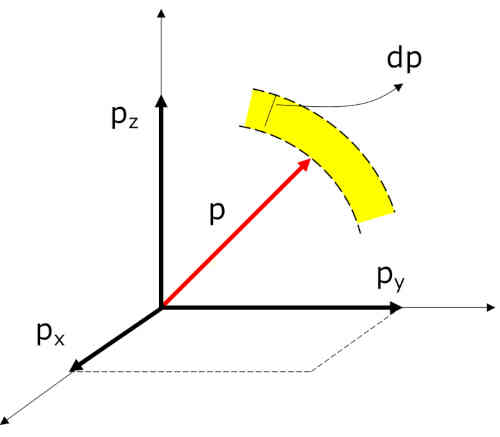
\includegraphics[width=0.3\textwidth]{immagini/volume-infinitesimo-sfera.jpg}
\caption{$\ud p_x \ud p_y \ud p_z$ è uguale al volume compreso tra due sfere concentriche di raggio $p$ e $p + \ud p$}
\label{fig:volume-infinitesimo-sfera}
\end{figure}

Sostituendo si trova la \emph{distribuzione di Fermi-Dirac}:
\begin{equation}\label{eq:fermi-dirac}
    N_p \ud p = \frac{8 \pi}{h^3} p^2 \ud p
\end{equation}
Si noti come essa \emph{non} dipenda da T. Per evidenziare l'emergenza del comportamento quantistico oltre la soglia di Fermi, si faccia riferimento alla figura~\ref{fig:distribuzione-fermi}, in cui è rappresentato l'indice ci occupazione dei livelli energetici $\Pi(p)$ in funzione di $p$.

\begin{figure}
\centering
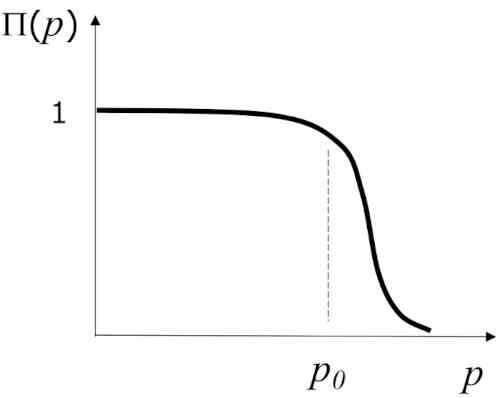
\includegraphics[width=0.3\textwidth]{immagini/distribuzione-fermi.jpg}
\caption{Indice di occupazione dei livelli energetici $\Pi(p)$ in funzione della quantità di moto $p$. $\Pi = 1$ corrisponde a un livello totalmente occupato.}
\label{fig:distribuzione-fermi}
\end{figure}

Integrando l'equazione~\eqref{eq:fermi-dirac} possiamo ottenere relazioni importanti in funzione del momento di Fermi. Si faccia attenzione al fatto che il massimo momento possibile è $p_0$, ovvero il momento di Fermi:
\[
N_e = \int_0^{p_0} \frac{8 \pi}{h^3} p^3 \ud p = \frac{8\pi}{3h^3} {p_0}^3
\]
dove $N_e$ rappresenta il numero di particelle per unità di volume. Sia $N_\textup{tot}$ il numero totale di particelle, $\langle m \rangle$ la massa media delle particelle, $M$ la massa totale e $V$ il volume. Si ha:
\[
N_e = \frac{N_\textup{tot}}{V} = \frac{M}{\langle m \rangle} \frac{1}{V} = \frac{\rho}{\mu_e H}
\]
dove è stata introdotta la densità $\rho$ e si è usata l'espressione~\eqref{eq:peso-molecolare-medio-definizione}.
Mettendo insieme le ultime due espressioni si ottiene:
\begin{equation}\label{eq:relazione-momento-fermi-densità}
    p_0 = \sqrt[3]{\dfrac{3h^3}{8\pi \mu_e H}} \rho^{1/3}
\end{equation}

Arrivati a questo punto, abbiamo tutti gli strumenti necessari per il calcolo della pressione. Come noto dalla meccanica statistica, conoscendo una distribuzione dei moduli di velocità, ipotizzando isotropia dello spazio, si può sempre trovare la pressione come:
\begin{equation}\label{eq:pressione-statistica}
    P = \frac{1}{3} m \int_0^\infty N(v) v^2 \ud v = \frac{1}{3m} \int_0^\infty N(p) p^2 \ud p
\end{equation}
e in generale bisogna distinguere tre casi:
\begin{description}
    \item[Gas perfetto] In questo caso la distribuzione di velocità da utilizzare è quella di Maxwell-Boltzmann. Integrando la~\eqref{eq:pressione-statistica} si ottiene la legge dei gas perfetti~\eqref{eq:gas-ideale}, in cui $\mu = \mu_e$.
    \item[Gas degenere non relativistico] La distribuzione di velocità è quella di Fermi Dirac. Si utilizza l'espressione classica per l'impulso, $p=mv$.
    \item[Gas degenere relativistico] La distribuzione di velocità è ancora quella di Fermi-Dirac, tuttavia si utilizza l'espressione relativistica per l'impulso, $p= \frac{m_e v}{\sqrt{1- (\frac{v}{c})^2}}$
\end{description}
Vediamo cosa si ottiene negli ultimi due casi.

\paragraph{Caso non relativistico}
In questo caso $p_0 \ll m_e c$ quindi possiamo scrivere $p=mv$ e integrare la~\eqref{eq:pressione-statistica} utilizzando la distribuzione di Fermi-Dirac~\eqref{eq:fermi-dirac}. Si ottiene:
\[
P = \dfrac{8\pi}{3h^3m} \int_0^{p_0} p^4 \ud p = \dfrac{8\pi}{3h^3m}\dfrac{{p_0}^5}{5}
\]
e sostituendo l'espressione per $p_0$ trovata precedentemente~\refeq{eq:relazione-momento-fermi-densità} otteniamo
\begin{equation}\label{eq:pressione-degenerazione-non-relativistica}
    P = k_1 \rho^{5/3}
\end{equation}
dove $k_1$ è una costante pari a:
\[
k_1 = 10^{13} {\mu_e}^{-5/3}
\]
Si noti come la pressione \emph{non} dipenda dalla temperatura. Questo fa sì che \emph{non} ci sia termoregolazione. Inoltre, la dipendenza dalla densità è maggiore rispetto che al gas perfetto (eq.~\eqref{eq:gas-ideale}).

\paragraph{Caso relativistico}
In questo caso si ha $p_0 \sim m_e c$ e bisogna utilizzare l'espressione relativistica dell'impulso:
\[
p= \dfrac{m_e v}{\sqrt{1- (\frac{v}{c})^2}}
\]
Sostituendo dentro~\eqref{eq:pressione-statistica} si ha:
\[
P = \dfrac{8\pi}{3mh^3} \int_0^{p_0} \dfrac{p^4 \ud p}{(1 + \dfrac{p^2}{m^2c^2})^{1/2}} = \dots = \dfrac{2\pi c}{3h^3}{p_0}^4
\]
dove si sono saltati i passaggi intermedi, riportati nel \emph{Cester}. Unendo l'ultima espressione con~\eqref{eq:relazione-momento-fermi-densità} si ottiene:
\begin{equation}\label{eq:pressione-degenerazione-relativistica}
    P = k_2 \rho^{4/3}
\end{equation}
con $k_2$ una costante pari a
\[
k_2 = 1.2 \cdot 10^{15} {\mu_e}^{-4/3}
\]
Nuovamente, non c'è dipendenza dalla temperatura e la dipendenza dalla densità è più forte che nel gas ideale~\eqref{eq:gas-ideale}.

\subsection{L'equazione in breve}
L'equazione di stato negli interni stellari~\eqref{eq:equazione-stato} ha tre contributi principali. Analizziamoli celermente.

\paragraph{Pressione di radiazione}
Il termine:
\[
P = \dfrac{aT^4}{3}
\]
rappresenta il contributo della pressione di radiazione per un corpo nero, secondo la eq.~\eqref{eq:pressione-radiazione} ottenuta integrando la distribuzione di Planck~\refeq{eq:corpo-nero}. È il contributo dei fotoni che compongono il gas stellare, i quali hanno un impulso e dunque esercitano una pressione.

\paragraph{Pressione degli ioni}
Il termine:
\[
\dfrac{k \rho T}{\mu_i H}
\]
è il contributo degli ioni nel materiale stellare, che pensiamo come a un plasma. Questi sono sempre approssimati come a un gas perfetto, infatti seguono la legge~\eqref{eq:gas-ideale}.

\paragraph{Pressione degli elettroni}
Il contributo:
\[
\begin{cases} 
    \dfrac{k \rho T}{\mu_e H} \\ 
    k_1 \rho^{5/3} \\ 
    k_2 \rho^{4/3}
    \end{cases}
\]
dipende dalla degenerazione del gas per ciò che concerne il contributo elettronico. Se il gas di elettroni è \emph{non} degenere, ovvero è un gas perfetto, segue la legge~\eqref{eq:gas-ideale}, dove $\mu = \mu_e$. Nel caso \emph{degenere} si distinguono due situazioni: la prima in cui si trattano le particelle come \emph{non} relativistiche, con un contributo alla pressione pari a $k_1 \rho^{5/3}$, e un secondo in cui si trattano le particelle come \emph{relativistiche}, con un contributo alla pressione pari a $k_2 \rho^{4/3}$.

\subsection{Contributo dominante}
Per descrivere lo stato della materia negli interni stellari, è utile utilizzare il \emph{diagramma} $\log \rho$ -- $\log T$. In pratica, note la densità e la temperatura di un certo strato di stella, questo piano permette di sapere quale componente di pressione prevale. Infatti, eguagliando tra loro diversi contributi di pressione, si ottengono delle rette che suddividono il piano in regioni in cui domina l'uno o l'altro contributo. Analizziamo i domini di demarcazioni per casi. Nella figura~\ref{fig:diagramma-logrho-logt} sono mostrati tutti i casi. Essa è riferita al nucleo stellare, in cui le temperature sono elevatissime, in superficie le temperature sono più basse.

\begin{figure}
\centering
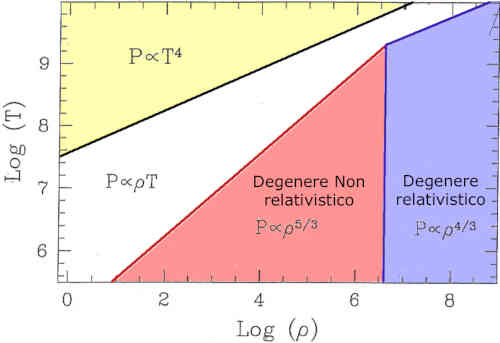
\includegraphics[width=0.5\textwidth]{immagini/piano-log-log.jpg}
\caption{Diagramma $\log \rho$ -- $\log T$. In giallo domina la pressione di radiazione, in bianco il gas non degenere (gas perfetto), in rosso il gas degenere non relativistico e in blu il gas degenere relativistico.}
\label{fig:diagramma-logrho-logt}
\end{figure}

\paragraph{Pressione di radiazione -- Pressione del gas perfetto}
Imponiamo $P_\textup{rad} = P_\textup{gas}$, uguagliando dunque l'eq.~\eqref{eq:pressione-radiazione} con l'eq.~\eqref{eq:gas-ideale}. In pratica sto considerando insieme il contributo degli ioni e degli elettroni, utilizzando $1/ \mu_i + 1 / \mu_e = 1 / \mu$
\[
\frac{1}{3} a T^4 = \frac{\kb \rho T}{\mu H}
\]
sviluppando si trova:
\[
T^3 = \dfrac{3\kb}{a\mu H} \rho
\]
da cui, passando ai logaritmi:
\[
\log T^3 = \log \rho + c
\]
e infine si può ricavare:
\begin{equation}\label{prad-pgas}
    \log T = \frac{1}{3} \log \rho + 7.57
\end{equation}
La regione in giallo del diagramma~\ref{fig:diagramma-logrho-logt} è quella in cui la pressione di radiazione domina su quella del gas perfetto, ovvero $P_\textup{rad} > P_\textup{gas}$

\paragraph{Pressione del gas degenere -- Pressione del gas perfetto}
Per sapere quando la pressione del gas degenere di elettroni prevale su quella di gas perfetto, uguagliamo la~\eqref{eq:gas-ideale} con la~\eqref{eq:pressione-degenerazione-non-relativistica}. Siccome la condizione di degenerazione riguarda solamente il contributo elettronico, nella parte del gas perfetto considero solo gli elettroni, per cui $\mu = \mu_e$:
\[
\frac{\kb \rho T}{\mu_e H} = k_1 \rho^{5/3}
\]
da cui si ottiene:
\[
T = \frac{k_1}{\kb} \rho^{2/3} \mu_e H
\]
e, passando ai logarirtmi:
\begin{equation}\label{eq:pgas-pdeg}
    \log T = \frac{2}{3} \log \rho + 4.88
\end{equation}
La regione in rosso del diagramma~\ref{fig:diagramma-logrho-logt} è quella in cui la pressione del gas degenere è maggiore della pressione del gas non degenere.

\paragraph{Pressione del gas degenere relativistico -- Pressione del gas degenere non relativistico}
Per sapere quando la pressione del gas degenere relativistico prevale su quella del gas degenere \emph{non} relativistico, uguagliamo la~\eqref{eq:pressione-degenerazione-non-relativistica} con la~\eqref{eq:pressione-degenerazione-relativistica}:
\[
k_1 \rho^{5/3} = P = k_2 \rho^{4/3}
\]
si trova:
\[
\rho^{1/3} = \frac{k_2}{k_1}
\]
da cui, passando ai logaritmi:
\begin{equation}\label{eq:pdegrel-pdegnonrel}
    \log \rho = 3 \log \frac{k_2}{k_1} = 6.6
\end{equation}
La pressione in blu del diagramma~\ref{fig:diagramma-logrho-logt} è quella in cui la pressione del gas degenere relativistico è maggiore di quella del gas degenere non relativistico.

\paragraph{Pressione del gas perfetto -- Pressione del gas degenere relativistico}
Analogamente a quanto fatto nel caso \emph{non} relativistico, ci sarà una regione del diagramma (per $\log \rho > 6.6$) in cui il gas può passare da \emph{non degenere} a \emph{degenere relativistico}. Per trovarla uguagliamo la~\eqref{eq:gas-ideale} con la~\eqref{eq:pressione-degenerazione-relativistica}:
\[
\frac{\kb \rho T}{\mu H} = k_2 \rho^{4/3}
\]
si trova:
\[
T = \frac{k_2 \mu_e H}{\kb} \rho^{1/3}
\]
e passando ai logaritmi:
\begin{equation}\label{eq:pgas-pdegrel}
    \log T = \frac{1}{3} \log \rho + 7.07
\end{equation}

\paragraph{Conclusioni}
La pressione di radiazione, siccome $p_\textup{rad} \propto T^4$, domina ad alte temperature. La pressione del gas degenere diventa dominante ad alte densità perché per avere degenerazione devo avere gli elettroni estremamente impacchettati nello spazio delle fasi, e ciò corrisponde ad elevate densità. Nei casi intermedi è sufficiente riferirsi al grafico~\ref{fig:diagramma-logrho-logt} per capire in quale situazione si è.

Riprenderemo questo utile diagramma successivamente, parlando di evoluzione stellare. Per ora sottolineamo solamente che le reazioni termonucleari sono attive solo se il gas si trova in condizioni di non degenerazione (gas perfetto).
\section{Equazione del bilancio energetico}\label{sec:bilancio-energetico}
L'\emph{equazione del bilancio energetico} esprime l'energia che emerge da ogni \emph{shell} della struttura stellare, essenzialmente dovuta alle reazioni termonucleari. Si può scrivere:
\begin{equation}\label{eq:bilancio-energetico}
    \dfrac{\ud L(r)}{\ud r} = 4 \pi r^2 \rho(r) \epsilon
\end{equation}
dove $L(r)$ è la luminosità emergente dalla sfera di raggio $r$ e $\epsilon$ l'energia prodotta da ogni shell per unità di tempo e di massa, $[\epsilon] = \si{erg.s^{-1}.g^{-1}}$.

\subsection{Ricavare l'equazione}
È semplice ricavare tale equazione. Consideriamo, infatti, l'usuale guscio di gas a una distanza $r$ dal centro. Sia $L(r)$ la luminosità emergente dalla porzione di stella delimitata dal guscio di raggio $r$ e analogamente per $L(r + \ud r)$. Possiamo scrivere:
\[
L(r + \ud r) - L(r) = \ud L(r) = 4 \pi \rho r^2 \ud r \epsilon
\]
dove $4 \pi \rho r^2 \ud r$ rappresenta la massa del guscio di sfera tra $r$ e $r + \ud r$ e $\epsilon$ è l'energia prodotta da ogni guscio per unità di tempo e di massa. Attenzione, \emph{non} si tratta dell'energia totale irradiata dalla stella. Moltiplicando le due quantità sopra si ottiene l'energia per unità di tempo, ovvero la luminosità (par.~\ref{sec:luminosità}).

Consideriamo un tipico profilo di luminosità radiale per una stella (fig.~\ref{fig:profilo-luminosità-sole}): la luminosità varia con $r$ sono in una regione ristretta della stella, corrispondente al suo centro, poi verso l'esterno diventa costante. All'esterno, secondo la eq.~\eqref{eq:bilancio-energetico} vale $\epsilon = 0$ e questo ci dice che tutta l'energia viene prodotta nelle regioni interne, come ci aspettiamo dal fatto che le reazioni termonucleari hanno bisogno di una elevata temperatura per poter avvenire. Tuttavia, le reazioni termonucleari \emph{non} sono le uniche a poter contribuire all'energia, in particolare anche la \emph{contrazione gravitazionale} può produrre energia, e tale contributo non è incluso nell'eq.~\eqref{eq:bilancio-energetico}. Per capire come la contrazione gravitazionale possa contribuire all'energia, bisogna far riferimento al \emph{teorema del viriale}.

\begin{figure}
\centering
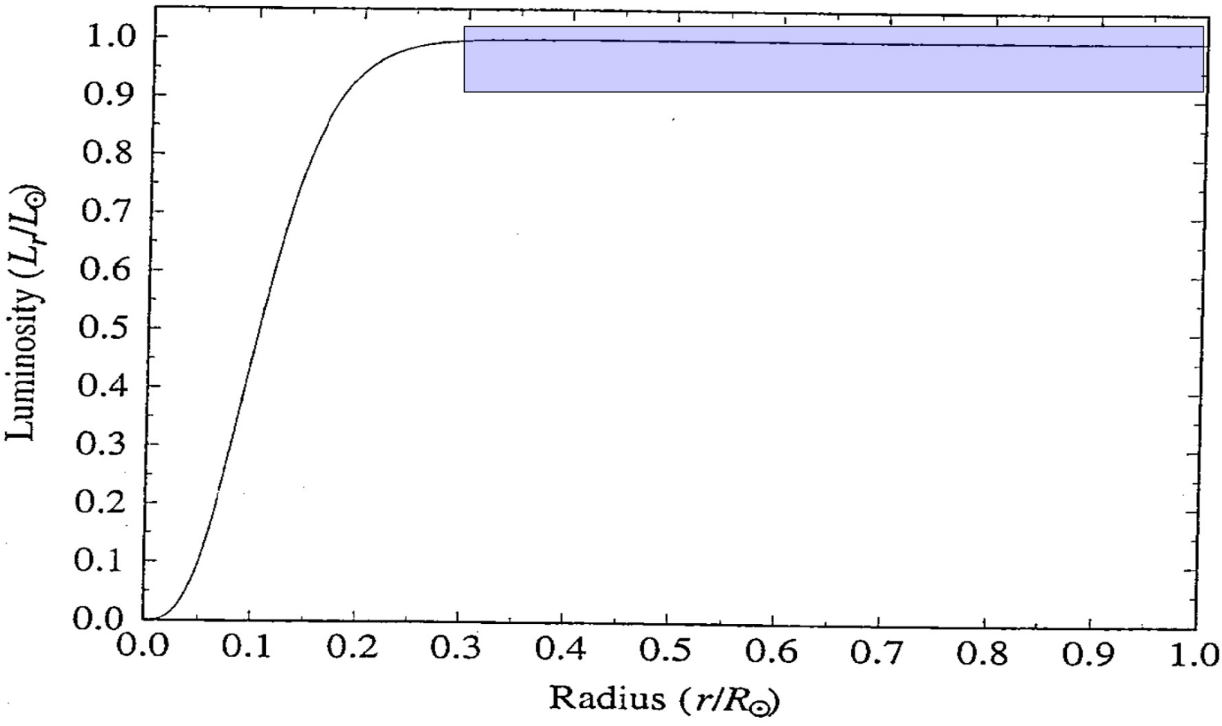
\includegraphics[width=0.4\textwidth]{immagini/profilo-luminosita-radiale-sole.png}
\caption{Profilo di luminosità radiale del Sole. Nella zona evidenziata si ha $L(r) = \textup{const}$, da cui, secondo eq.~\eqref{eq:bilancio-energetico}, $\epsilon = 0$. Questo ci dice che negli strati esterni della stella non viene prodotta energia e le reazioni termonucleari sono concentrate nell'interno stellare, dove infatti le temperature sono più elevate.}
\label{fig:profilo-luminosità-sole}
\end{figure}

\subsection{Teorema del viriale}
Per ogni sistema in equilibrio di particelle auto--gravitanti, come nel caso delle strutture stellari, vale il \emph{teorema del viriale}:
\begin{equation}\label{eq:teorema-viriale}
    2K + \Omega = 0
\end{equation}
dove $K$ è l'energia cinetica del sistema e $\Omega$ l'energia potenziale. L'eq.~\eqref{eq:teorema-viriale} dice sostanzialmente che a una contrazione ($\ud \Omega < 0$) segue un aumento dell'energia cinetica, e quindi un aumento della temperatura. Scrivendo inoltre l'energia totale del sistema come $U = K + \Omega$, si ha
\[
U = - \frac{\Omega}{2} + \Omega \implies U = \frac{\Omega}{2}
\]
ovvero a una contrazione ($\ud \Omega < 0$) segue una diminuzione dell'energia totale del sistema ($\ud U < 0$).

Le due relazioni considerate precedentemente:
\begin{equation}\label{eq:viriale-differenziale}
\ud U = \frac{\ud \Omega}{2} \qquad \ud K = - \frac{\ud \Omega}{2}
\end{equation}
mostrano che in ogni contrazione ($\ud \Omega$) \emph{metà} dell'energia è \emph{emessa} e \emph{metà} dell'energia è usata per incrementare la temperatura. Possiamo riformulare quanto detto in un altro modo: ogni perdita di energia totale $\ud U$ dovuta a emissioni genera una contrazione del sistema, che produce anche un incremento della temperatura interna.

Come stimare il contributo della contrazione gravitazionale alla luminosità di una stella? Se fosse elevato andrebbe corretta l'eq.~\eqref{eq:bilancio-energetico}. Per capirlo utilizziamo la~\eqref{eq:viriale-differenziale} per scrivere
\[
L = \frac{\ud U}{\ud t} = \frac{1}{2} \abs*{\frac{\ud \Omega}{\ud t}}
\]
ovvero abbiamo scritto la luminosità in funzione della variazione di energia potenziale dovuta alla contrazione gravitazionale. Integriamo nel tempo:
\[
\int_0^t L \ud t = \frac{1}{2} \abs{\Omega}
\]
A questo punto consideriamo un tempo caratteristico $t^*$ approssimando $L$ con un suo valore medio costante $\Bar{L}$. Si può scrivere:
\[
\Bar{L} \cdot t^* = \frac{1}{2} \frac{GM^2}{R}
\]
dove abbiamo sostituito $\Omega$ con l'espressione del potenziale gravitazionale. Abbiamo trovato il così detto \emph{tempo di Kelvin-Helmoltz}:
\begin{equation}\label{eq:tempo-kelvin-helmoltz}
    t^* = \dfrac{GM^2}{2LR}
\end{equation}
Esso ci dà una \emph{stima} del tempo durante il quale una stella è in grado di  mantenere costante la sua luminosità per effetto della sola contrazione gravitazionale. 

Facciamo una stima per il nostro Sole introducendo nella~\eqref{eq:tempo-kelvin-helmoltz} i parametri $G = \SI{6.67e-8}{cm^3.g^{-1}.s^{-2}}$, $\si{\solarmass} \sim \SI{2e33}{g}$, $\si{\solarradius} \sim \SI{7e10}{cm}$ e $\si{\solarluminosity} \sim \SI{4e33}{erg.s^{-1}}$. Si ottiene:
\[
{t^*}_{\textup{Sole}} \sim \SI{1.5e7}{anni}
\]
ovvero, per il nostro Sole, l'energia gravitazionale può mantenere costante la luminosità per circa $15$ milioni di anni (sono molto pochi). Questo farebbe pensare che la fonte principale di luminosità sia la contrazione gravitazionale per il nostro Sole, ma si rivela un'idea sbagliata perché attraverso fonti geologiche si è mostrato che l'età del Sole è dell'ordine dei miliardi di anni e che in tale tempo la luminosità del Sole è rimasta praticamente invariata. Questo dimostra che il grosso del contributo alla luminosità del Sole proviene dalle reazioni termonucleari e quindi l'equazione~\eqref{eq:bilancio-energetico} risulta soddisfacente anche se non contempla il contributo della contrazione di gravità.
\section[Gradiente radiativo]{Gradiente radiativo e criterio di Schwarzschild}\label{sec:gradiente-radiativo}
L'equazione del \emph{gradiente radiativo} fornisce il profilo radiale delle variazioni di $T$ all'interno della stella. Si può scrivere:
\begin{equation}\label{eq:gradiente-radiativo}
    \dfrac{\ud T}{\ud r}\Big|_\textup{rad} = - \dfrac{3 \kappa \rho}{4 \pi r^2} \dfrac{L(r)}{4 a c T^3}
\end{equation}
Essa mostra che l'opacità e il flusso radiativo determinano quanto rapidamente $T$ varia con $r$.

Utilizzando questa equazione è possibile determinare quando c'è convezione nella stella, utilizzando il seguente \emph{criterio di Schwarzscild}:
\begin{equation}\label{eq:criterio-schwarzscild}
    \text{se} \quad \abs*{\dfrac{\ud T}{\ud r}}_\textup{rad} > \abs*{\dfrac{\ud T}{\ud r}}_\textup{ad} \implies \text{c'è convezione.}
\end{equation}
in particolare, quando il criterio è verificato avverrà la convezione.

\subsection{Ricavare l'equazione}
Per trovare il gradiente radiativo prima di tutto ricaviamo il gradiente di pressione di radiazione, derivando rispetto a $r$ l'espressione~\eqref{eq:pressione-radiazione}. Si ottiene:
\[
\dfrac{\ud P_\textup{rad}}{\ud r} = \frac{4}{3} a T^3 \dfrac{\ud T}{\ud r}
\] 
d'altra parte, il gradiente di radiazione dipende anche dall'\emph{opacità} e dal \emph{flusso} di radiazione. Si ricorda che l'opacità $\kappa$ era stata introdotta nell'eq.~\eqref{eq:trasporto-radiativo} del par.~\ref{sec:soluzioni-trasporto-radiativo}, mentre il flusso, $F_\textup{rad}$, è definito dall'eq.~\eqref{eq:flusso}. In particolare, senza dare ulteriori specificazioni, possiamo esprimere il gradiente della pressione di radiazione come:
\[
\dfrac{\ud P_\textup{rad}}{\ud r} = -\dfrac{\kappa \rho}{c} F_\textup{rad}
\]
e mettendo insieme le utlime due relazioni si ottiene:
\[
\dfrac{\ud T}{\ud r}\Big|_\textup{rad} = - \dfrac{3}{4ac} \dfrac{\kappa \rho}{T^3} F_\textup{rad}
\]
con
\[
F_\textup{rad} = \dfrac{L_r}{4 \pi r^2}
\]
da cui segue immediatamente la~\eqref{eq:gradiente-radiativo}. Come già detto, l'equazione fornisce il profilo radiale delle variazioni di $T$ con $r$ e mostra come l'opacità $\kappa$ e il flusso radiativo $F_\textup{rad}$ influiscono sulla rapidità di variazione di $T$ con $r$.

Il gradiente di temperatura ha un impatto cruciale sul meccanismo preponderante di trasporto di energia all'interno della struttura stellare. Introduciamo brevemente i meccanismi di trasporto di energia.

\subsection{Meccanismi di trasporto di energia}
I tre meccanismi di trasporto in una stella sono il \emph{trasporto radiativo}, \emph{convettivo} e \emph{conduttivo}. Di seguito ne sono elencate le principali proprietà:
\begin{description}
    \item[trasporto conduttivo] I principali responsabili di questo meccanismo sono gli \emph{elettroni} ed è efficiente solo se il gas è \emph{degenere}. Infatti, in condizione di non degenerazione, ovvero se il gas è perfetto, il libero cammino medio è molto piccolo e un elettrone cede subito energia. Come visto, nel caso di un gas degenere (par.~\ref{sec:principio-indeterminazione}) le celle dello spazio delle fasi sono impacchettati in modo che i livelli energetici più bassi sono pieni, quindi gli elettroni percorrono una grande distanza prima di cedere energia (la quale deve essere di un ordine pari al primo livello energetico libero, che tendenzialmente sarà alto). In questo caso il trasporto conduttivo è efficiente e in questo modo è possibile trasportare l'energia dall'interno verso l'esterno. Tuttavia, questo meccanismo di trasporto non è quello preponderante.
    \item[trasporto radiativo] Esso è dovuto alla radiazione trasportata dai \emph{fotoni}.
    \item[trasporto convettivo] Con la convezione ho un rimescolamento del \emph{gas} e dunque di porzioni di gas con composizioni chimiche diversa. Siccome la struttura chimica è cruciale per stabilire la struttura stellare e la sua evoluzione, è importante capire se è in atto questo meccanismo di trasporto energetico.
\end{description}

\subsection{Criterio di Schwarzschild}
Come evidenziato nel paragrafo precedente, stabilire se sia in corso un meccanismo di convezione è importante per realizzare dei corretti modelli della struttura stellare e dunque per capire correttamente l'evoluzione di una stella. Come discriminante si può utilizzare il \emph{criterio di Schwarzschild} (eq.~\eqref{eq:criterio-schwarzscild}). Semplicemente si tratta di un confronto tra il \emph{gradiente radiativo} di temperatura e un valore di riferimento chiamato \emph{gradiente adiabatico}. In particolare, nelle regioni in cui il gradiente radiativo è maggiore del gradiente adiabatico, è in corso la convezione, come stabilito dalla~\eqref{eq:criterio-schwarzscild}. Il gradiente adiabatico dipende dai calori specifici del gas e si può scrivere:
\begin{equation}\label{eq:gradiente-adiabatico}
    \dfrac{\ud T}{\ud r}\Big|_\textup{ad} = \Bigl(1- \frac{1}{\gamma}\Bigr) \dfrac{T}{P} \dfrac{\ud P}{\ud r}
\end{equation}
dove
\[
\gamma =\frac{c_P}{c_V} = \frac{5}{3}
\]

\begin{figure}
\centering
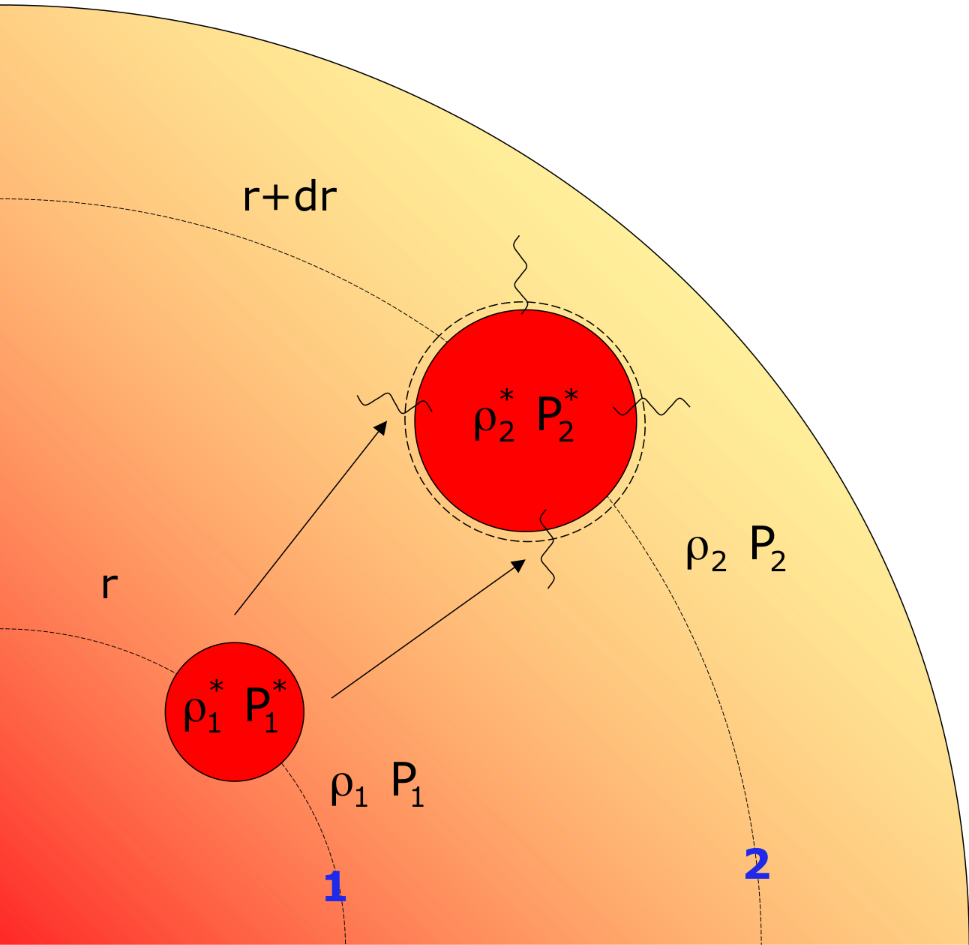
\includegraphics[width=0.3\textwidth]{immagini/criterio-schwarzscild.png}
\caption{Raffigurazione del criterio di Schwarzscild. Se la bolla si sposta dalla posizione $1$ e $2$, può avvenire la convezione solamente se ${\rho_2}^* < \rho_2$. In caso contrario siamo in presenza di equilibrio stabile e la bolla viene respinta verso la posizione iniziale.}
\label{fig:criterio-schwarzscild}
\end{figure}

Per capire il criterio~\eqref{eq:criterio-schwarzscild} consideriamo (fig.~\ref{fig:criterio-schwarzscild}) una bolla di gas in una posizione $1$ a distanza $r$ rispetto al centro, di densità ${\rho_1}^*$ e pressione interna ${P_1}^*$. Siano $\rho_1$ e $P_1$ rispettivamente la densità e la pressione dell'ambiente circostante la bolla in quella posizione. Immagino che essa si sposti in una posizione $2$ a distanza $r + \ud r$ dal centro, avendo una nuova densità ${\rho_2}^*$ e una nuova pressione interna ${P_2}^*$. Analogamente a prima, siano $\rho_2$ e $P_2$ rispettivamente la densità e la pressione dell'ambiente circostante la bolla in quella posizione. Ho convezione nella stella solo se l'equilibrio è instabile, perché in caso di equilibrio stabile la bolla tenderebbe a tornare nella posizione originaria $1$ e non sarebbe possibile lo spostamento di porzioni di gas nella stella. La condizione di equilibrio dipende dal rapporto della densità interna della bolla nel secondo caso, ${\rho_2}^*$, e la densità del gas circostante, $\rho_2$. In particolare:
\begin{subequations}
\label{eq:relazioni-densità-schwarzscild}
\begin{align}
  \text{se} \quad {\rho_2}^* &> \rho_2 \implies \text{la bolla torna nella posizione iniziale $1$.} \\
  \text{se} \quad {\rho_2}^* &< \rho_2 \implies \text{la bolla continua ad andare verso l'alto.} 
\end{align}
\end{subequations}
ed è semplice tradurre le espressioni~\eqref{eq:relazioni-densità-schwarzscild} in termini dei gradienti di temperatura, ottenendo~\eqref{eq:criterio-schwarzscild}.

\subsection{Esempio per il gas perfetto}
\begin{figure}
\centering
\subfloat[][\emph{Caso in cui avviene la convezione: modulo del gradiente radiativo maggiore del gradiente adiabatico.} \label{fig:criterio-schwarzscild-gas-perfetto1}]
{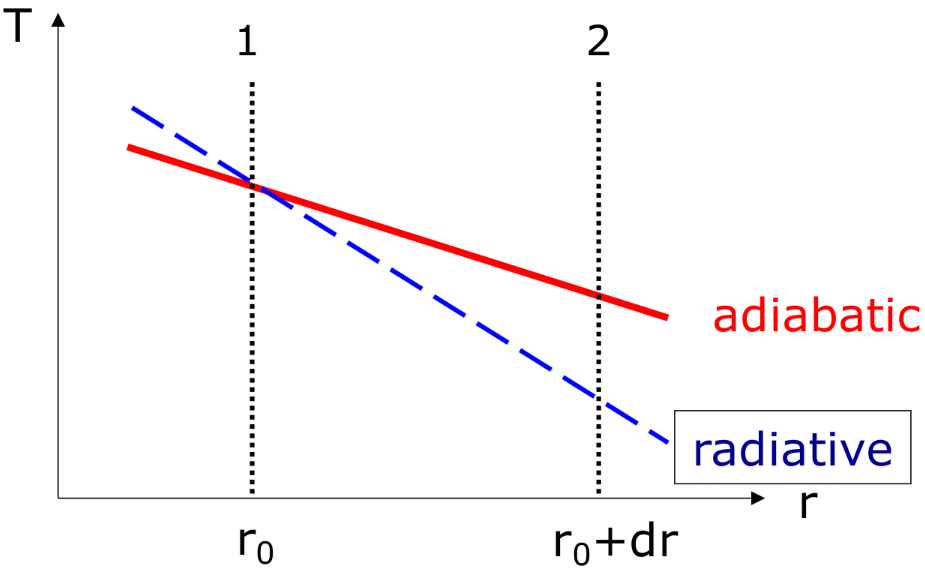
\includegraphics[width=.35\textwidth]{immagini/criterio-schwarzscild-gas-perfetto1.png}} \qquad
\subfloat[][\emph{Caso in cui non avviene la convezione: modulo del gradiente radiativo minore del gradiente adiabatico.}\label{fig:criterio-schwarzscild-gas-perfetto2}]
{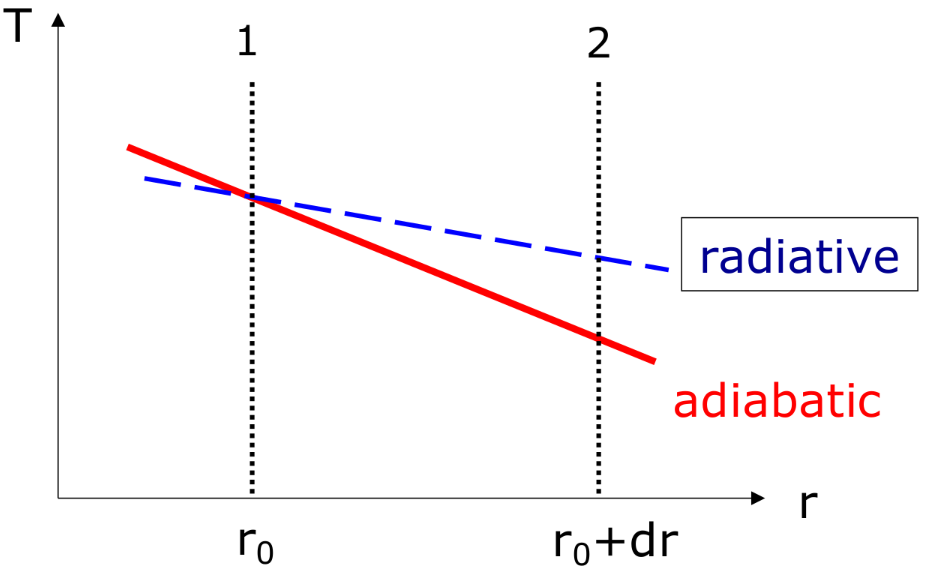
\includegraphics[width=.35\textwidth]{immagini/criterio-schwarzscild-gas-perfetto2.png}} 
\caption{Applicazione del criterio di Schwarzscild nel caso di un gas perfetto.}
\label{fig:criterio-schwarzscild-gas-perfetto}
\end{figure}

Per capire meglio le condizioni~\eqref{eq:relazioni-densità-schwarzscild} e il criterio di Schwarzscild~\eqref{eq:criterio-schwarzscild}, consideriamo il caso di un gas perfetto, in cui vale la legge~\eqref{eq:gas-ideale}. Si faccia riferimento alla figura~\ref{fig:criterio-schwarzscild-gas-perfetto}. Consideriamo un caso in cui è possibile la convezione e un caso in cui essa non è possibile

\paragraph{Convezione possibile}
Nel caso illustrato nella figura~\ref{fig:criterio-schwarzscild-gas-perfetto1} la convezione è possibile, infatti in quel caso si ha:
\[
abs*{\dfrac{\ud T}{\ud r}}_\textup{rad} > \abs*{\dfrac{\ud T}{\ud r}}_\textup{ad}
\]
si faccia attenzione al fatto che nel criterio di Schwarzscild~\eqref{eq:criterio-schwarzscild} i gradienti sono espressi in modulo, quindi bisogna guardare la pendenza in modulo delle rette. In particolare, la bolla di gas di sposta da $r_0$ fino a $r_0 + \ud r$ e nella posizione $r_0 + \ud r$ possiede una temperatura (curva rossa -- profilo adiabatico) maggiore dell'ambiente circostante (curva blu -- profilo radiativo). Per un gas perfetto, secondo la ~\eqref{eq:gas-ideale}, a fissata pressione, a una maggiore temperatura corrisponde una densità più bassa. Quindi la bolla possiede una densità più bassa dell'ambiente circostante e tende a continuare il suo moto verso l'esterno. È dunque possibile la convezione.

\paragraph{Convezione impossibile}
Nel caso illustrato nella figura~\ref{fig:criterio-schwarzscild-gas-perfetto2} la convezione \emph{non} è possibile, infatti in quel caso si ha:
\[
abs*{\dfrac{\ud T}{\ud r}}_\textup{rad} < \abs*{\dfrac{\ud T}{\ud r}}_\textup{ad}
\]
In particolare, la bolla di gas di sposta da $r_0$ fino a $r_0 + \ud r$ e nella posizione $r_0 + \ud r$ possiede una temperatura (curva rossa -- profilo adiabatico) minore dell'ambiente circostante (curva blu -- profilo radiativo). Per un gas perfetto, secondo la ~\eqref{eq:gas-ideale}, a fissata pressione, a una minore temperatura corrisponde una densità più alta. Quindi la bolla possiede una densità più alta dell'ambiente circostante e viene respinta verso la posizione iniziale a $r_0$.


Si faccia riferimento alla figura
Si faccia riferimento alla figura~\ref{fig:criterio-schwarzscild-gas-perfetto2}

\subsection{Gradiente di pressione e scala logaritmica}
Il criterio di Schwarzscild è spesso scritto usando il gradiente di temperatura riferito alla \emph{pressione} invece che al raggio e in scala logaritmica. Questo perché la temperatura è intimamente connessa con la pressione.
\begin{equation}
    \dfrac{\ud T}{\ud P} \dfrac{P}{T} = \dfrac{\ud \log T}{\ud \log P} \equiv \nabla
\end{equation}
L'impiego di $\nabla$ semplifica la formulazione del criterio. Ad esempio, possiamo riscrivere l'espressione del gradiente adiabatico~\eqref{eq:gradiente-adiabatico} nella seguente maniera:
\[
\Bigl(1- \frac{1}{\gamma}\Bigr) = \dfrac{P}{T} \dfrac{\ud r}{\ud P} \dfrac{\ud T}{\ud r}\Big|_\textup{ad} = \dfrac{P}{T} \dfrac{\ud T}{\ud P}\Big|_\textup{ad}
\]
da cui:
\begin{equation}
    \nabla_\textup{ad} = \Bigl(1- \frac{1}{\gamma}\Bigr)
\end{equation}
che è semplicemente un numero. In particolare, con $\gamma = 5/3$ si ottiene $\nabla_textup{ad} = 0.4$ ed è possibile riscrivere il criterio di Schwarzscild~\eqref{eq:criterio-schwarzscild} nella seguente materia:
\begin{equation}\label{eq:criterio-schwarzscild-nabla}
    \text{se} \quad \nabla_\textup{rad} > \nabla_\textup{ad} \implies \text{c'è convezione.}
\end{equation}
Si faccia riferimento alla figura~\ref{fig:criterio-schwarzscild-nabla} per un sunto del criterio.

\begin{figure}
\centering
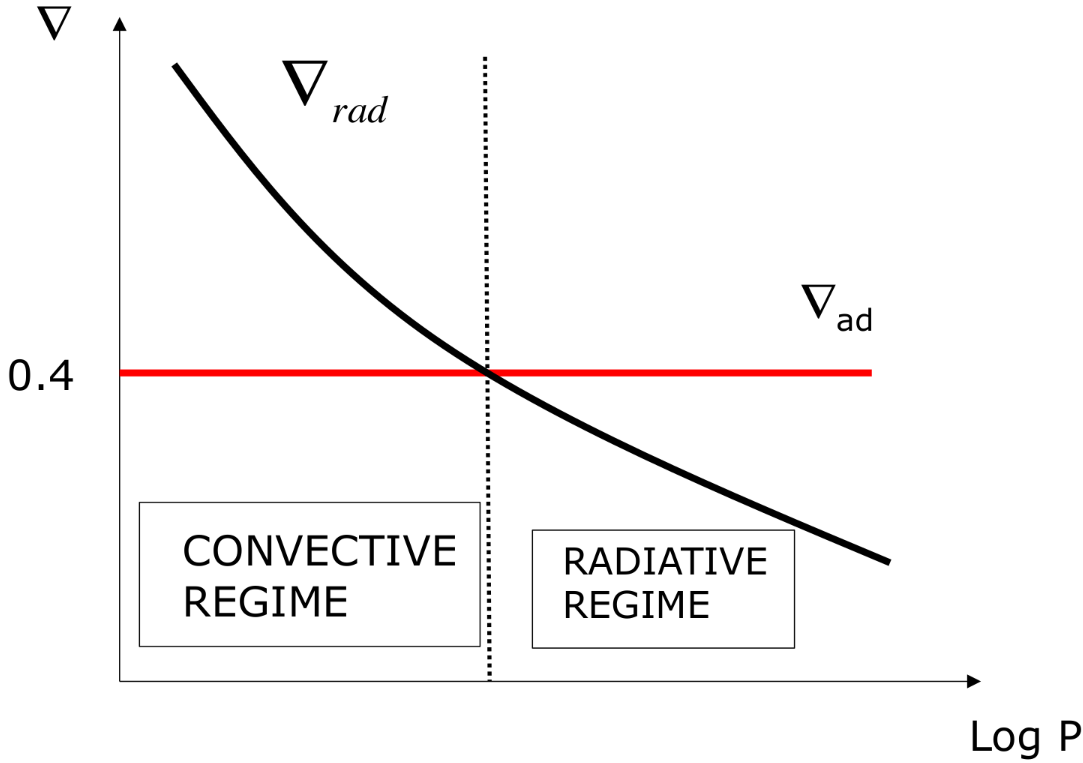
\includegraphics[width=0.4\textwidth]{immagini/criterio-schwarzscild-nabla.png}
\caption{Raffigurazione del criterio di Schwarzscild utilizzando $\nabla$.}
\label{fig:criterio-schwarzscild-nabla}
\end{figure}
\input{capitoli/stelle/opacità.tex}
\section[Reazioni Termonucleari]{Produzione di energia tramite reazioni termonucleari}\label{sec:reazioni-termonucleari}
Le \emph{reazioni termonucleari} sono la principale fonte di energia in una stella. La \emph{fusione} di elementi leggeri in elementi più pesanti produce non solo \emph{energia}, ma anche \emph{nuovi elementi}. Come nel caso dell'opacità i processi sono molto complessi e utilizzeremo solamente delle equazioni approssimate. Si faccia attenzione al fatto che i processi di fusione termonucleare coinvolgono solamente i \emph{nuclei} dell'atomo, perché le temperature sono così elevate ($T > \SI{e6}{K}$) che tutti gli atomi si possono considerare completamente ionizzati.

L'equazione di produzione di energia attraverso \emph{reazioni termonucleari} appare nella seguente maniera:
\begin{equation}\label{eq:reazioni-termonucleari}
    \epsilon = \epsilon(X, \rho, T) 
    \begin{cases} \epsilon_{PP} = \epsilon_1 \rho X^2 T_6^\alpha \quad \alpha \in [3.5 - 6] \\ 
    \epsilon_{CN} = \epsilon_2 \rho X X_{CN} T_6^\beta \quad \beta \in [13 - 20] \\ 
    \epsilon_{3\alpha} = \epsilon_3 \rho^2 Y^3 T_8^\gamma \quad \gamma \in [20 - 30] \\
    \end{cases}
\end{equation}
È dapprima necessario introdurre dei concetti di base sulla reazioni termonucleari.

\subsection{Ripasso di fisica nucleare}
\paragraph{Numero atomico e numero di massa}
Nel presente paragrafo si farà una veloce rassegna dei concetti di fisica nucleare utili per proseguire il discorso.

Ogni elemento chimico è univocamente identificato dal suo \emph{numero atomico} $Z$, corrispondente al numero di protoni nel nucleo. Il \emph{peso atomico} $A$ è il numero totale di nucleoni, ovvero la somma di protoni e neutroni. Gli \emph{isotopi} hanno stesso $Z$ ma diverso $A$.

\paragraph{Difetto di massa}
Nelle reazioni di fusione termonucleare, nuclei di elementi leggeri si fondono tra loro generando nuclei di elementi più pesanti ($Z$ più alto) ed energia. Pertanto, a causa della nota relazione massa-energia, la somma delle masse dei nuclei leggeri che fondono tra loro è maggiore della massa del nucleo più pesante che viene generato, e si può scrivere:
\begin{equation}\label{eq:difetto-massa}
    E = \Delta m \, c^2
\end{equation}
Guardando la carta dei nuclidi che rappresenta l'energia di legame per nucleone (fig.~\ref{fig:energia-legame}), possiamo stabilire che è grazie alle reazioni di fusione del nucleo delle stelle che sono stati prodotti tutti gli elementi più pesanti dell'elio ($Z=2$) fino al ferro ($Z=26$), come verrà riassunto successivamente.

\paragraph{Energia di legame}
All'interno del nucleo atomico, i nucleoni sono legati tra loro dalla \emph{forza forte}, la quale agisce su distanze estremamente piccole ($\sim \SI{e-12}{cm}$ -- $\SI{e-13}{cm}$). La massa totale del nucleo è sempre minore della somma di tutti i nucleoni che lo costituiscono. Questo si spiega attraverso il difetto di massa, eq.~\eqref{eq:difetto-massa}, e permette di definire l'\emph{energia di legame} come:
\begin{equation}\label{eq:energia-legame}
    E(Z,N) = \bigl[ Z m_p + N m_n - m(Z,n) \bigr] \, c^2
\end{equation}

con $Z$ il numero di protoni, $N$ il numero di neutroni, $m_p = \SI{1.672e-24}{g}$ la massa del protone, $m_n = \SI{1.675e-24}{g}$ la massa del neutrone e $m(Z,n)$ la massa del nucleo. Questo significa che quando si forma un nuovo nucleo stabile, una certa frazione di massa viene trasformata in energia secondo la~\eqref{eq:energia-legame}, ovvero, $E(Z,N)$ è l'energia che viene prodotta quando si forma un nuovo nucleo stabile, ovvero $E(Z,N)$ è l'energia che bisogna fornire ad un nucleo per spaccarlo nei singoli nucleoni che lo costituiscono.

\paragraph{Energia di legame per nucleone dei nuclidi stabili}

\begin{figure}
    \centering
    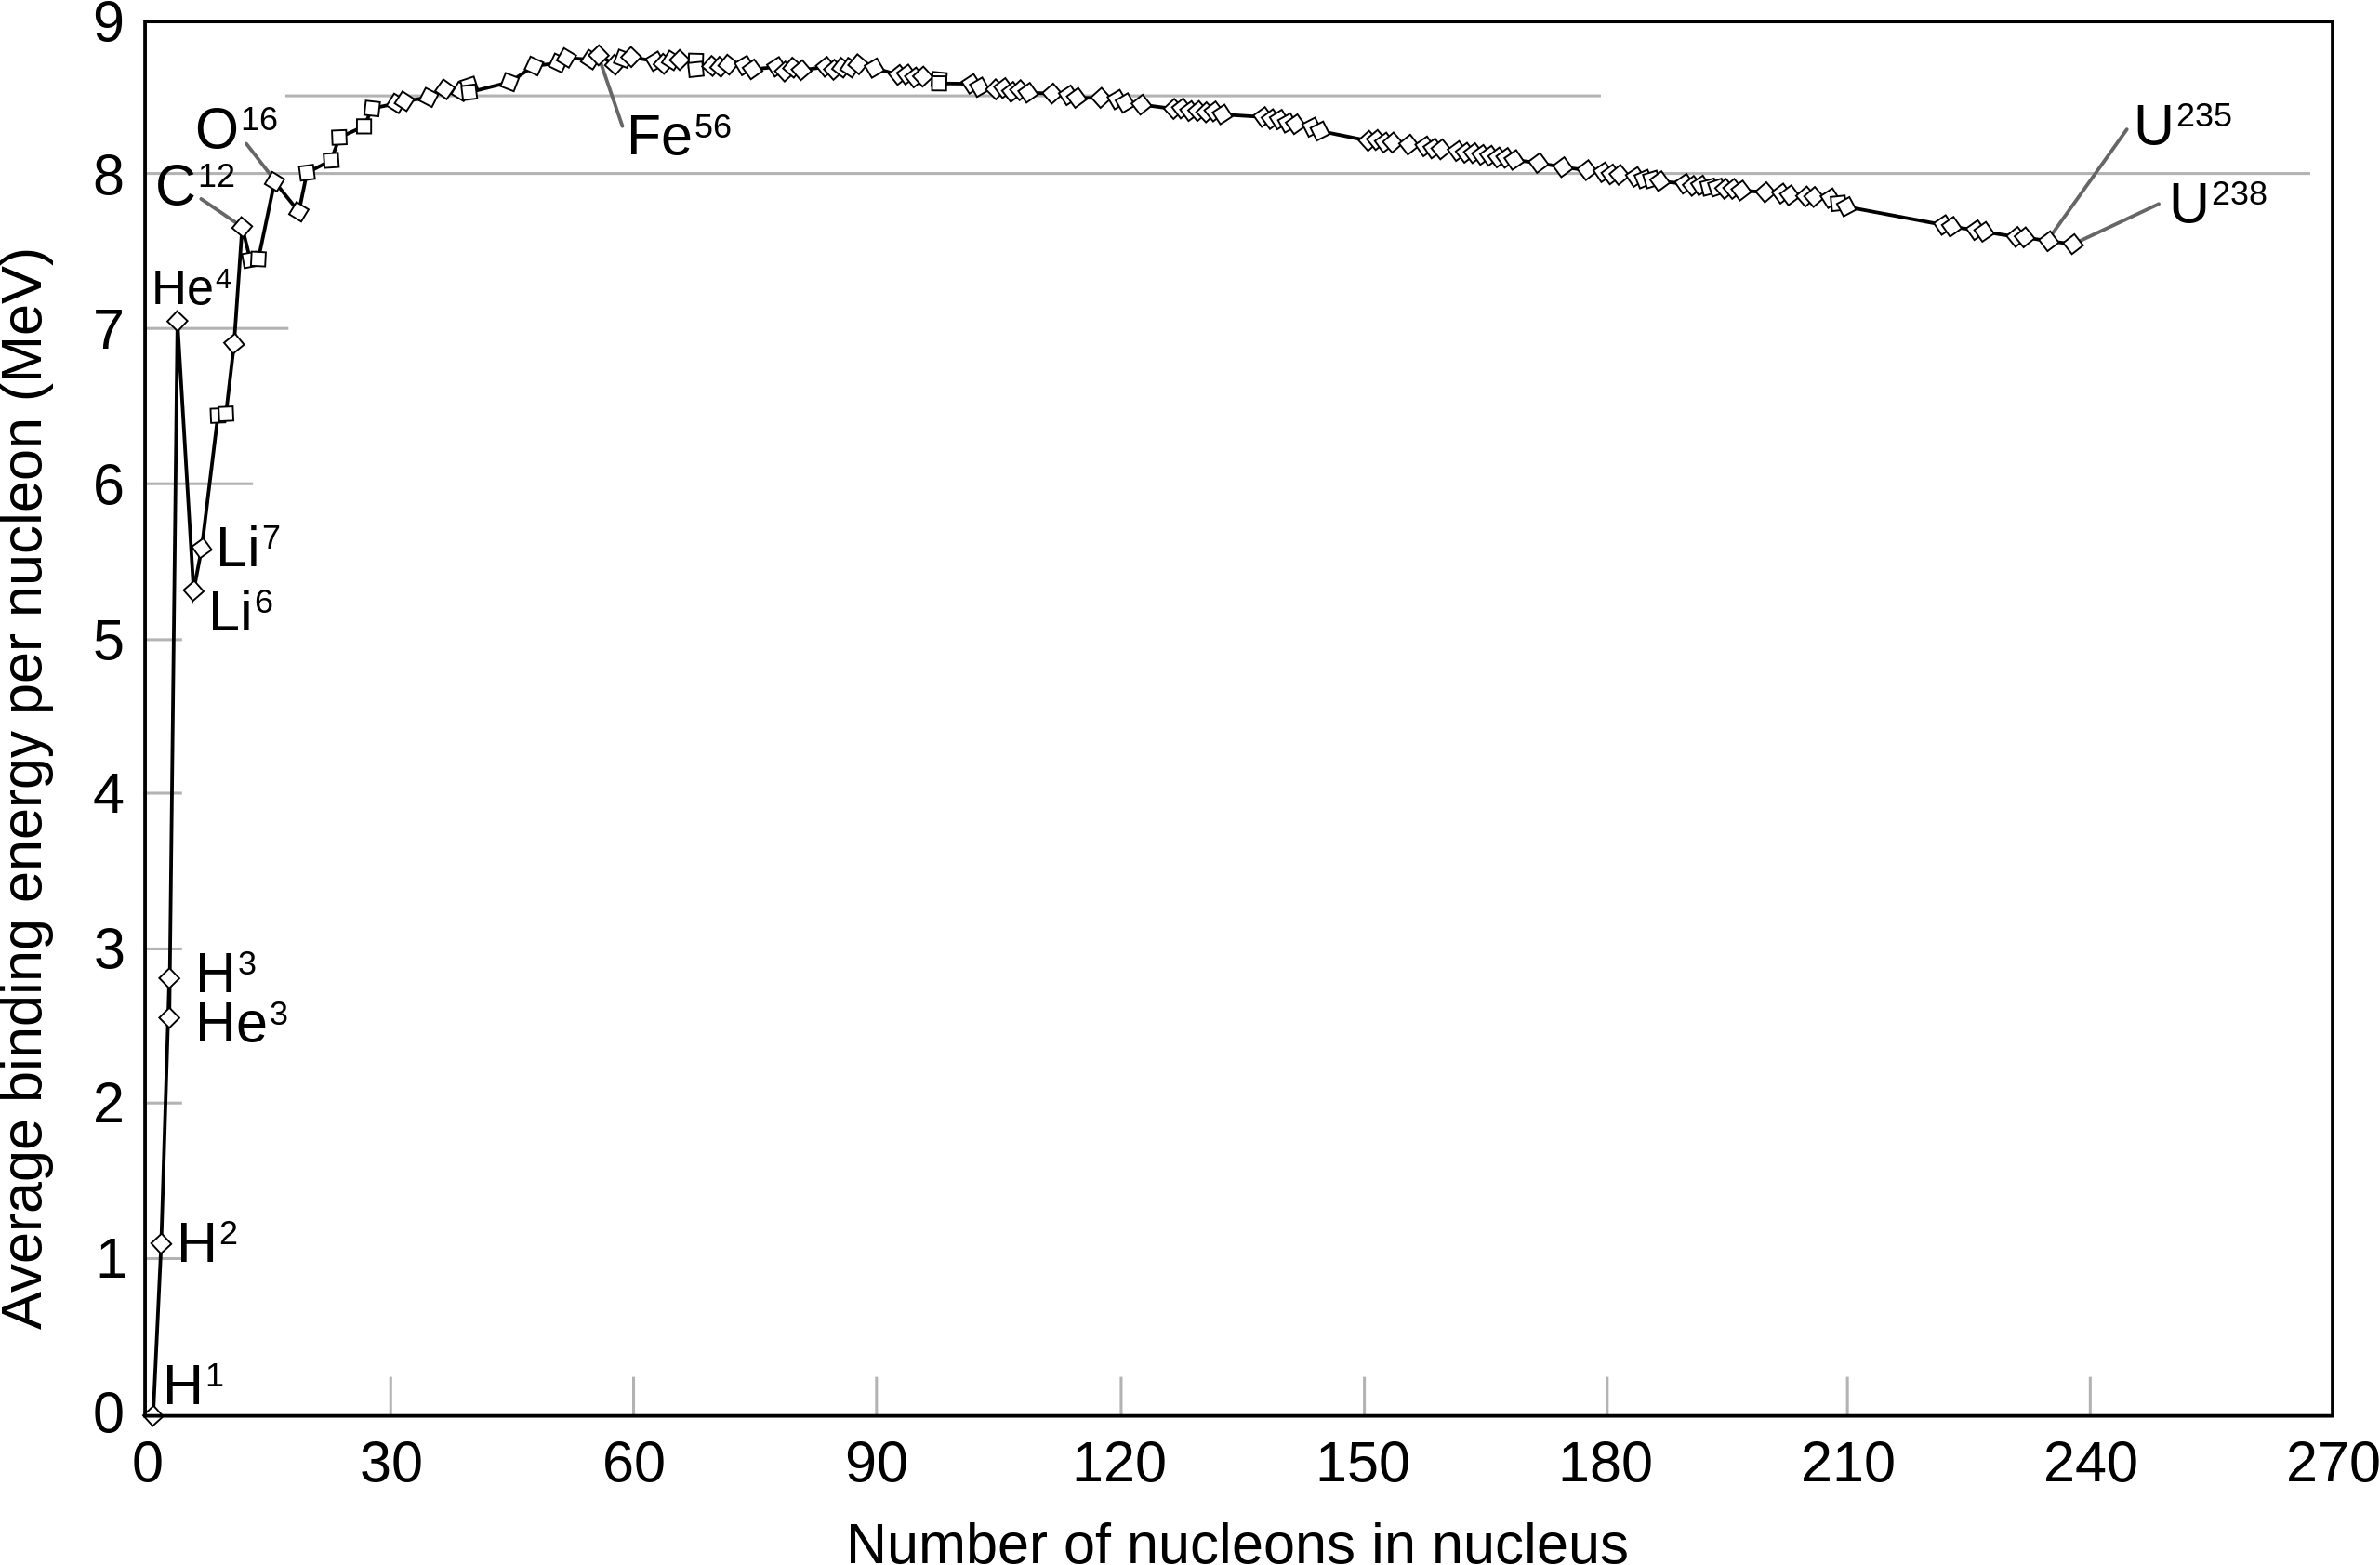
\includegraphics[width=0.7\textwidth]{immagini/energia-legame.png}
    \caption{Energia di legame media per nucleone. Si noti come \ce{^4He} sia particolarmente stabile, fino al ferro domina la fusione e dopo il ferro domina la fissione.}
    \label{fig:energia-legame}
\end{figure}

Consideriamo l'\emph{energia di legame media per nucleone}, plottata in fig.~\ref{fig:energia-legame}, e corrispondente, secondo la~\eqref{eq:energia-legame} a $E(Z,N) / A$. Dalla figura possiamo trarre alcune considerazioni generali:
\begin{itemize}
    \item ci sono configurazioni nucleari particolarmente stabili quali \ce{^4He}, \ce{^{12}C}, \ce{^{16}O} \dots
    \item a parte queste eccezioni, l’energia di legame media per nucleone, $E/A$, ha un andamento regolare. Aumenta rapidamente con il numero di nucleoni fino ad un valore dell’ordine degli $\SI{8}{Mev}$ per poi diminuire assai lentamente (\emph{proprietà di saturazione}).
    \item i nuclei più stabili sono il \ce{^{56}Fe} e il \ce{^{62}Ni}. Ciò significa che i nuclei pesanti alla sua destra possono raggiungere configurazioni più stabili ($B/A$ più elevato) diminuendo il numero di nucleoni $A$, ovvero frazionandosi in nuclei più piccoli. Mentre i nuclei leggeri alla sua sinistra possono raggiungere configurazioni più stabili ($B/A$ più elevato) aumentando $A$, ovvero aggregandosi in nuclei più grandi. Detto in altri termini ciò significa che le reazioni di fissione dei nuclei pesanti e quelle di fusione dei nuclei leggeri sono esoenergetiche ovvero producono energia qualora si sia in grado di innescarle.
    \item dal punto precedente consegue che le reazioni di \emph{fusione dei nuclei leggeri} e \emph{fissione dei nuclei pesanti} costituiscono la doppia opportunità offerta dalla fisica nucleare per la produzione di energia.
\end{itemize}

\paragraph{Barriera di potenziale ed effetto tunnel}
Da un punto di vista \emph{classico} la reazione di fusione avviene se due nuclei riescono ad avvicinarsi a meno della distanza $R_0$ necessaria per far entrare in gioco le interazioni forti, ovvero solo dopo aver superato la barriera di potenziale in fig.~\ref{fig:barriera-potenziale}

\begin{figure}
    \centering
    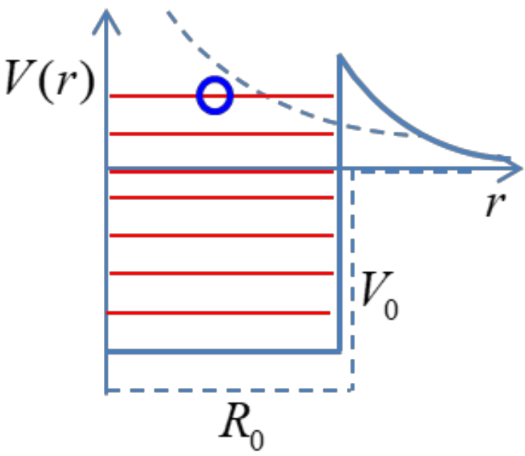
\includegraphics[width=0.3\textwidth]{immagini/barriera-potenziale.png}
    \caption{Barriera di potenziale. È data dalla sovrapposizione del potenziale attrattivo della forza forte, che agisce per $r < R_0$ e della forza repulsiva Coulombiana, che agisce per $r > R_0$ e vale $E_c = Z_1 Z_2 e^2 / r$.}
    \label{fig:barriera-potenziale}
\end{figure}

Facendo una stima molto rozza, possiamo trovare che la barriera di potenziale è circa $1000$ volte superiore all'energia termica media delle particelle, quindi, anche ad elevatissime temperature, è molto improbabile che le reazioni possano avvenire. Dal punto di vista quantistico questo si spiega con il così detto \emph{effetto tunnel}.

\paragraph{Pricnicpali catene di fusione termonucleare nelle stelle}
Di seguito sono elencate le principali catene di fusione nelle stelle, le quali saranno approfondite nei successivi paragrafi:
\begin{description}
    \item[Catena PP] Processo di bruciamento dell'idrogeno. È un processo di cattura protonica. Avviene per $T \simeq \SI{e7}{K}$.
    \item[Catena CNO] Processo di bruciamento dell'idrogeno. È un processo di cattura protonica. Avviene per $T \simeq \SI{1.8e7}{K}$.
    \item[Catena 3-alpha] Processo di bruciamento dell'elio. Avviene per temperature $T \simeq \SI{1.5e8}{K}$.
    \item[Cattura alpha] Il carbonio e materiali più pesanti catturano particelle $\alpha$ per produrre materiali più pesanti. Avviene per $T > \SI{5e8}{K}$.
\end{description}

\subsection{Catena protone--protone}\label{sec:catena-pp}
\paragraph{Catena PPI}
La catena \emph{protone--protone PPI} è rappresentata in fig.~\ref{fig:catena-pp1}. È una reazione di bruciamento dell'idrogeno e dà elio. Può essere scritta nella seguente maniera:
\reaction[re:pp1]{H^1 + H^1 -> H^2 + e^+ + $\nu$}
\reaction[re:pp2]{H^2 + H^1 -> He^3 + $\gamma$}
\reaction[re:pp3]{He^3 + He^3 -> He^4 + H^1 + H^1}
ovvero, in definitiva da \ce{4 H} ottengo \ce{1 He^4}, e siccome \ce{1 He^4} pesa meno di \ce{4 H}, dall'eq.~\eqref{eq:difetto-massa} possiamo stabilire che la reazione è \emph{esotermica}.

\begin{figure}
    \centering
    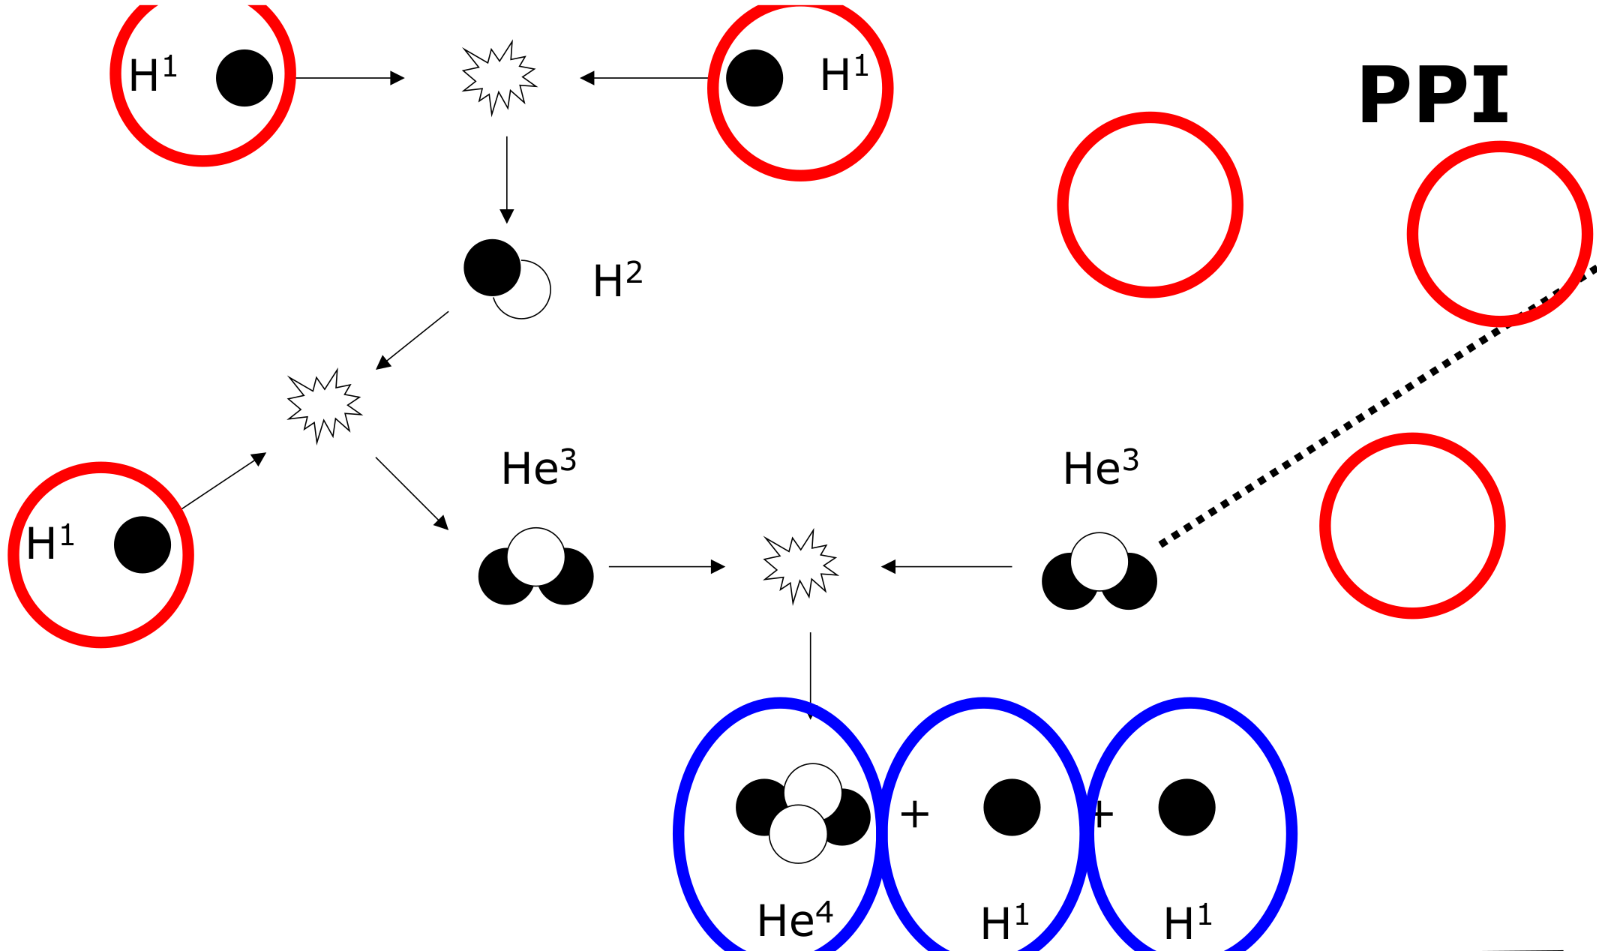
\includegraphics[width=0.5\textwidth]{immagini/catena-pp1.png}
    \caption{Catena protone-protone (PPI).}
    \label{fig:catena-pp1}
\end{figure}

Facciamo una stima dei contributi energetici. Il neutrino $\nu$ porta un contributo energetico \emph{negativo}, perché avendo una scarsa interazione con la materia tendono a sfuggire dalla struttura stellare. Senza aggiungere ulteriori specificazioni, si ricordi che, tenuti in considerazione tutti i contributi, l'energia totale prodotta dalla reazione PPI è:
\begin{equation}\label{eq:energia-pp1}
    E_\textup{PPI} = \SI{26.2}{MeV} = \SI{4.2e-5}{erg}
\end{equation}

Senza scendere troppo nei dettagli, evidenziamo che il \emph{tempo scala} della reazione~\ref{re:pp1} è $t_1 = \SI{1.4e9}{yr}$, il tempo scala della reazione~\ref{re:pp2} è $t_2 = \SI{6}{s}$ e il tempo scala della reazione~\ref{re:pp3} è $t_3 = \SI{e6}{yr}$. Dunque, ricordando che la \emph{probabilità} che avvenga la reazione è proporzionale all'inverso del tempo scala, possiamo stabilire che la prima reazione è molto improbabile che avvenga, mentre la seconda è molto probabile. In particolare, concentriamoci sulla prima reazione (~\ref{re:pp1}). Essa trasforma due protoni liberi (\ce{H}) in un nucleo costituito da un protone e un neutrone (\ce{H^2}). Significa che uno dei due protoni si è trasformato in neutrone. Quindi, affinché la reazione possa avvenire, è necessario che ci sia un \emph{decadimento $\beta$}, espresso dalla seguente equazione:
\reaction[re:decadimento-beta+]{p^+ -> n + e^+ + $\nu$}
Tuttavia, il decadimento $\beta^+$ per un protone libero è essenzialmente impossibile, poiché la massa del protone è minore della massa del neutrone (eq.~\eqref{eq:difetto-massa}). Nonostante ciò, nel nucleo delle stelle tale reazione può avvenire poiché ci sono tantissimi protoni, dunque anche se la probabilità è bassissima, questa è compensata dall'elevato numero. 

D'altra parte, il \emph{decadimento $\beta^-$}, secondo il quale un neutrone decade in protone, è un processo spontaneo, in quanto il suo tempo scala è dell'ordine di $\SI{800}{s}$ e tende ad eliminare tutti i neutroni liberi:
\reaction[re:decadimento-beta-]{n -> p^+ + e^- + $\nu$}
Tuttavia negli interni stellari possono comunque esserci neutroni liberi, i quali contribuiscono alla formazione di elementi più pesanti, come vedremo successivamente.

\paragraph{Catena PPII e PPIII}
Consideriamo le reazioni~\ref{re:pp1} e~\ref{re:pp2}. Con una probabilità $P_1 = 69 \%$ può avvenire, successivamente, la reazione~\ref{re:pp3}, dando origine alla catena PPI. Tuttavia, non si tratta dell'unica possibilità. Infatti, con una probabilità residua del $31\%$, può avvenire la seguente reazione:
\reaction[re:ppsecondaria]{He^3 + He^4 -> Be^7 + $\gamma$}
Se inizialmente prevale la PPI, dopo un po' che questa è attiva l'ambiente si popola di \ce{He^2} e può facilmente avvenire la~\ref{re:ppsecondaria}, che produce energia. Se è attivo tale canale, quasi sempre la catena prosegue con la PPII (fig.~\ref{fig:catena-pp2}), con una probabilità $P_2=99.7\%$, nella seguente maniera:
\reaction[re:ppII1]{Be^7 + e^- -> Li^7 + $\nu$}
\reaction[re:ppII2]{Li^7 + H^1 -> Be^8}
\reaction[re:ppII3]{Be^8 -> 2 He^4 + $\gamma$} 
In particolare, nella~\ref{re:ppII3} il \ce{Be^8} è instabile e si spacca in due nuclei di \ce{He^4}, producendo energia, a causa della sua elevata stabilità, come si nota anche in fig.~\ref{fig:energia-legame}.

\begin{figure}
    \centering
    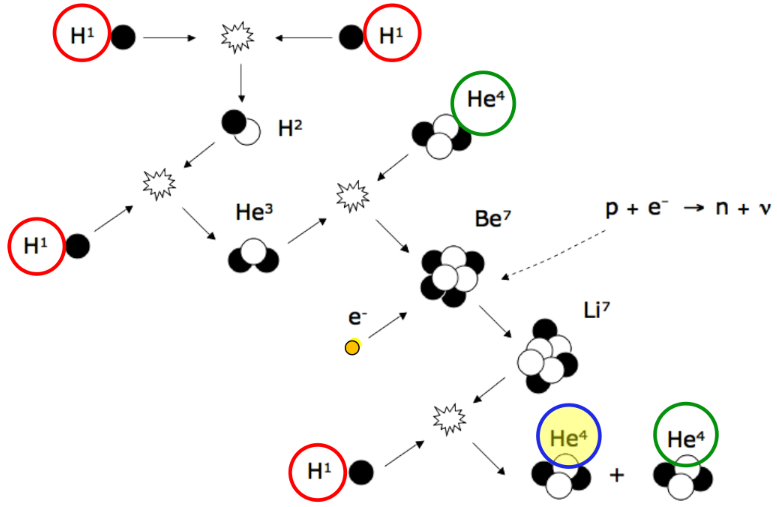
\includegraphics[width=0.5\textwidth]{immagini/catena-pp2.png}
    \caption{Catena protone-protone (PPII).}
    \label{fig:catena-pp2}
\end{figure}

Con una probabilità residua di $P_3 = 0.3\%$, la \ref{re:ppsecondaria} può proseguire con una catena PPIII (fig.~\ref{fig:catena-pp3}), nella seguente maniera:
\reaction[re:ppIII1]{Be^7 + H^1 -> B^8 + $\gamma$}
\reaction[re:PPIII2]{B^8 -> Be^8 + e^+ + $\gamma$}
\reaction[re:PPIII3]{Be^8 -> 2 He^4 + $\gamma$}

\begin{figure}
    \centering
    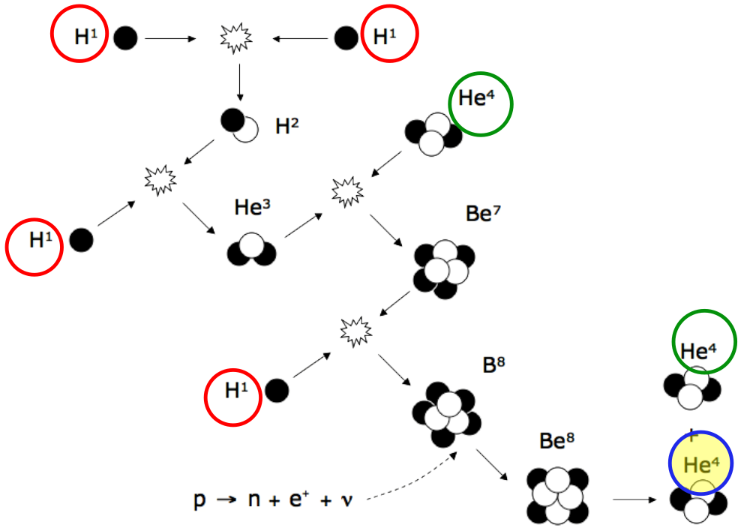
\includegraphics[width=0.5\textwidth]{immagini/catena-pp3.png}
    \caption{Catena protone-protone (PPIII).}
    \label{fig:catena-pp3}
\end{figure}

In tutti i casi, tuttavia, brucio \ce{4 H} per generare \ce{1 He^4}, producendo un'energia di $\sim \SI{20}{Mev}$. In particolare si ha: $E_\textup{PPI} = \SI{26.2}{Mev}$, $E_\textup{PPII} = \SI{25.7}{Mev}$ e $E_\textup{PPIII} = \SI{19.3}{Mev}$. 

\subsection{Catena CNO}\label{sec:catena-cno}
Un'altra possibile catena di bruciamento dell'idrogeno, è la così detta \emph{catena CNO}, detta anche \emph{CN--NO}. A differenza della precedente (par.~\ref{sec:catena-pp}), richiede la presenza di carbonio, azoto e ossigeno. Si noti che questi ultimi elementi \emph{non} sono prodotti dalla catena di reazione, ma devono essere già presenti nel gas, agendo come catalizzatori. Il ciclo principale della catena è raffigurato in fig.~\ref{fig:catena-cno} e può essere sintetizzato dalle seguenti reazioni:
\reaction[re:cno1]{C^{12} + H^1 -> N^{13} + $\gamma$}
\reaction[re:cno2]{N^{13} -> C^{13} + e^+ + $\nu$}
\reaction[re:cno3]{C^{13} + H^1 -> N^{14} + $\gamma$}
\reaction[re:cno4]{N^{14} + H^1 -> O^{15} + $\gamma$}
\reaction[re:cno5]{O^{15} -> N^{15} + e^+ + $\nu$}
\reaction[re:cno6]{M^{15} + H^1 -> C^{12} + He^4}

\begin{figure}
    \centering
    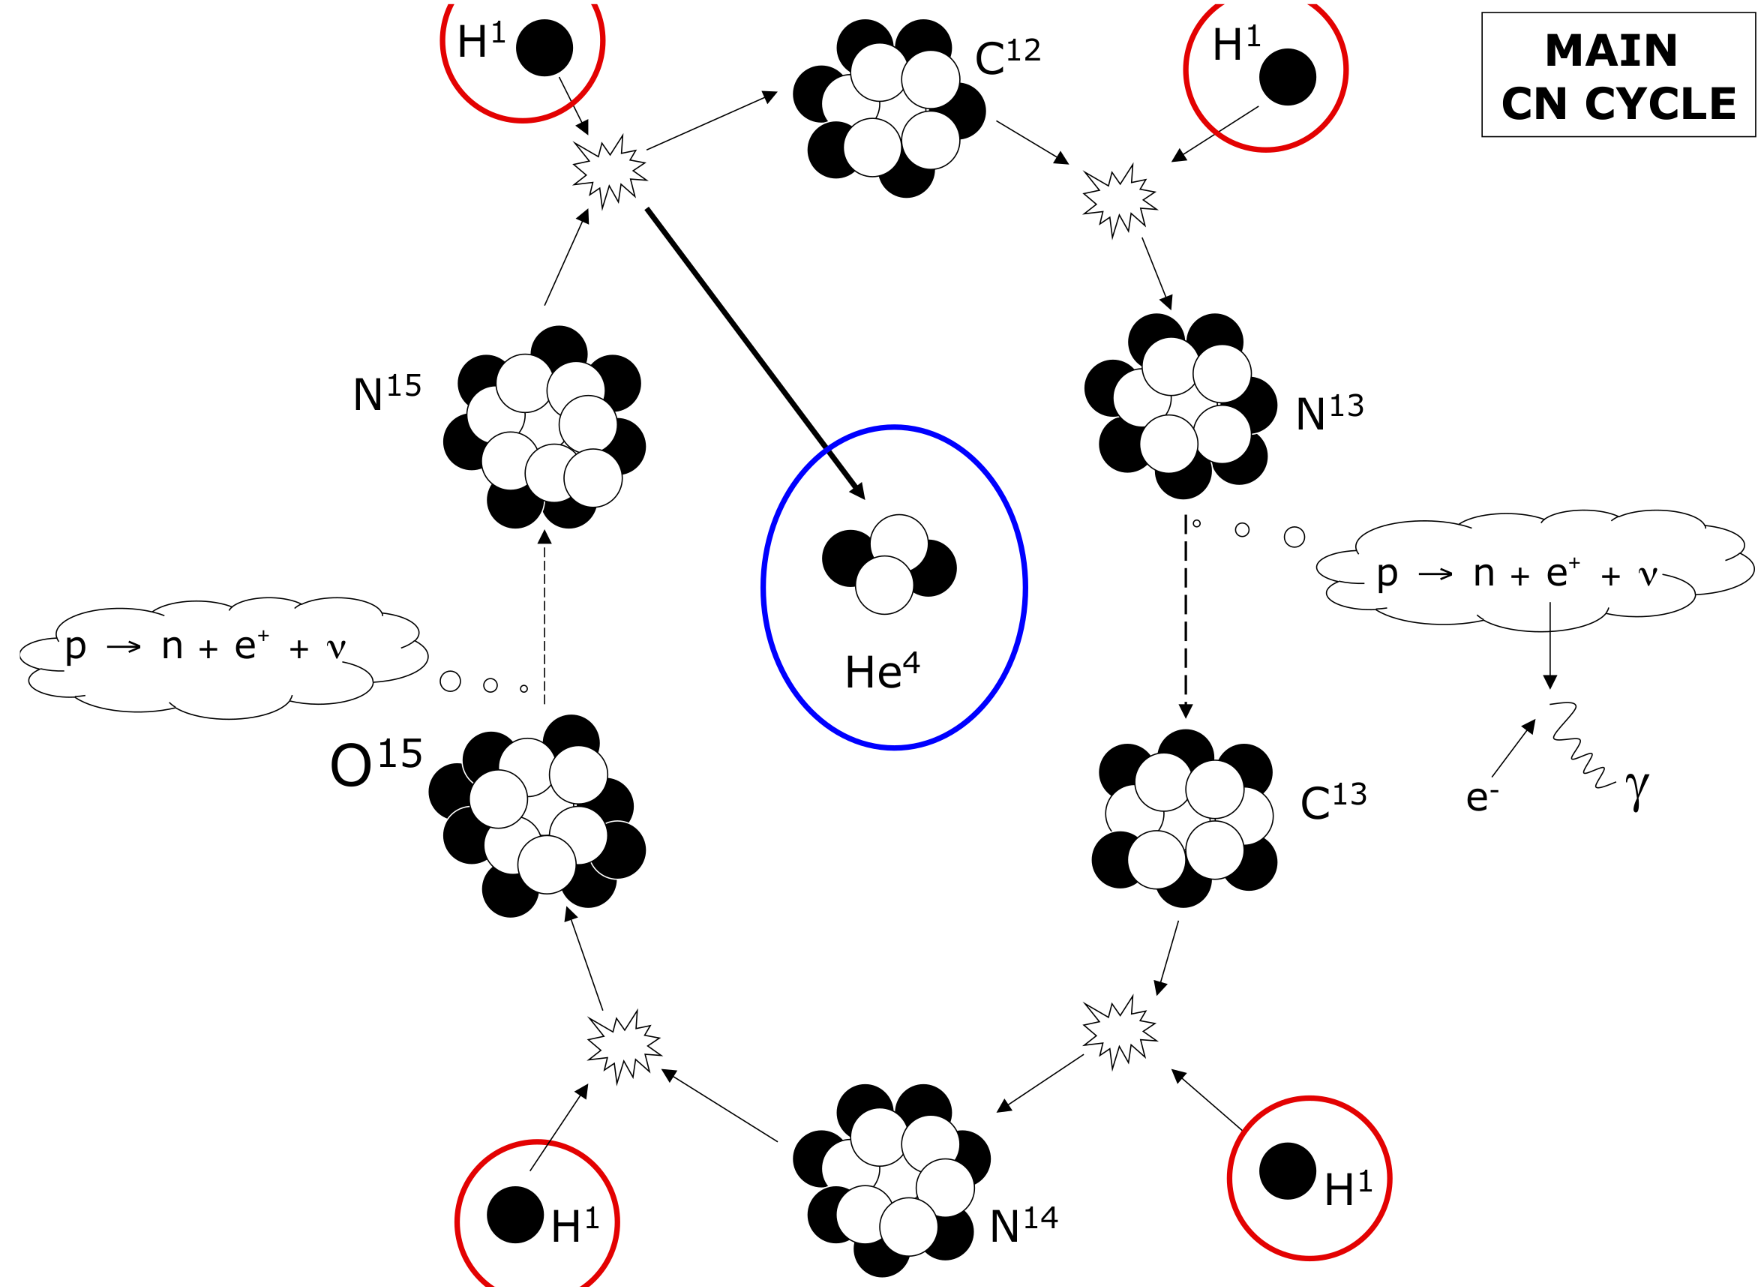
\includegraphics[width=0.5\textwidth]{immagini/catena-cno.png}
    \caption{Catena CN--NO. Partendo da \ce{C^{12}}, la parte sinistra rappresenta il ramo rapido, mentre la parte destra, che parte da \ce{N^{14}} rappresenta il ramo lento.}
    \label{fig:catena-cno}
\end{figure}

In totale il ciclo utilizza \ce{4 H} e genera \ce{1 He^4}. Facendo un computo delle energie, si ha:
\begin{equation}\label{eq:energia-cno}
E_\textup{CNO} = \SI{25}{MeV} \simeq \SI{2e-5}{erg}
\end{equation}
dello stesso ordine di grandezza dell'energia delle catene PP~\eqref{eq:energia-pp1}. Senza approfondire tutti i tempi scala, si sottolinea che quello della reazione~\ref{re:cno4} è dell'ordine di $\SI{3.2e8}{yr}$, dividendo la catena in un ramo rapido (da~\ref{re:cno1} a~\ref{re:cno4}) e un ramo lento (da~\ref{re:cno4} a~\ref{re:cno6} e nuovamente~\ref{re:cno1}). Quindi, nelle stelle in cui avviene il ciclo CNO mi aspetto che, se il materiale processato va verso la superficie per convezione, deve esserci una variazione delle abbondanze chimiche. In particolare, mi aspetto che l'abbondanza del carbonio diminuisca e quella dell'azoto e dell'ossigeno aumentino. Infine, sottolineiamo che questa reazione è un prototipo di reazione di cattura protonica.

\subsection{Il problema dell'elio}
Dopo aver visto alcune catene di bruciamento dell'idrogeno, soffermiamoci sul \emph{problema dell'elio}. Esso consiste nel fatto che l'abbondanza di \ce{He} che si misura nell'universo è troppo alta per essere spiegata solo in base al bruciamento dell'idrogeno negli interni stellari.

Considerato che nell'universo si misura un'abbondanza di \ce{He} pari a
\begin{equation}\label{eq:abbondanza-elio-misurata}
    Y \sim 0.24 - 0.28
\end{equation}

Stimiamo, quindi, quanto \ce{He} può essere stato prodotto dalle stella da quando si è formato l'universo, ovvero in un tempo di Hubble ($t_H \sim \SI{13}{Gyr}$), facendo un conto per la Via Lattea, della quale conosciamo la massa $M_G$ e la luminosità $L_G$
\[
M_G \sim \SI{e12}{\solarmass} \qquad M_G \sim \SI{e11}{\solarluminosity}
\]
e supponendo che tutta la luminosità della Galassia venga dal bruciamento di idrogeno in elio e che sia rimasta sempre costante. In questo modo dovrei sovrastimare il valore reale. Ricordando che la luminosità è l'energia prodotta per unità di tempo (par.~\ref{sec:luminosità}), per $L_G$, in un tempo $t_H$ si trova un'energia:
\[
E_\textup{tot} \simeq L_G t_H \sim \SI{1.6e62}{erg}
\]
che rappresenta l'energia totale prodotta dal bruciamento di \ce{H} in \ce{He} da quando si è formata la Galassia. Considerato che l'energia di legame di un nucleo di \ce{He} è
\[
E_\textup{b, He} \sim \SI{4.5e-5}{erg}
\]
e che può essere pensata come l'energia prodotta dal bruciamento di 4 nuclei di \ce{H} in un nucleo di \ce{He}, possiamo trovare il numero di atomi di \ce{He^4} che si sono formati dalla formazione della Galassia:
\[
N_\textup{He} = \frac{E_\textup{tot}}{E_\textup{b, He}} \simeq \SI{3.5e66}{}
\]
Possiamo pensare questo numero come il numero di reazioni di bruciamento di idrogeno che sono avvenute. Ora, dalla massa di un atomo di elio, $m_\textup{He} \sim \SI{6.64e-24}{g}$, possiamo ricavare la massa totale di \ce{He} prodotta in un tempo di Hubble:
\[
M_\textup{He} = N_\textup{He} m_\textup{He} \sim \SI{2.4e43}{g}
\]
Infine, usando $M_G$ possiamo trovare la frazione in massa di elio prodotta dalle Via Lattea da quando l'universo si è formato:
\begin{equation}\label{eq:abbondanza-elio-stimata}
Y = \frac{M_\textup{He}}{M_G} \sim 0.01
\end{equation}
Confrontando la~\eqref{eq:abbondanza-elio-misurata} con la~\eqref{eq:abbondanza-elio-stimata}, notiamo come l'abbondanza di elio misurata sia circa 20 volte maggiore di quella stimata. Questo significa che una frazione rilevante di \ce{He} deve essere stata prodotta da un altro processo, molto più efficiente e primordiale: si tratta del \emph{Big Bang}. Infatti, un punto rilevante che esso riesce a spiegare è la formazione di \emph{deuterio} (\ce{H^2}), processo molto difficile nelle stelle a causa della carenza di neutroni liberi, che decadono spontaneamente in protoni per il decadimento $\beta^-$ (\ref{re:decadimento-beta-}). Tuttavia, nei primi minuti successivi al Big Banda, c'erano molti neutroni liberi disponibili, e dunque la seguente catena di reazioni spiega la formazione di una grande quantità di elio subito dopo il Big Bang:
\reaction[re:bb1]{n + p -> H^2 + $\gamma$}
\reaction[re:bb2]{H^2 + H^2 -> He^3 + n}
\reaction[re:bb3]{He^3 + n -> H^3 + p}
\reaction[re:bb4]{H^2 + H^3 -> He^4 + n}
Tale \emph{nucleosintesi primordiale} si è fermata all'elio e non ha prodotto elementi più pesanti, poiché le reazioni successive di cattura neutronica o protonica avrebbero prodotto elementi instabili. In definitiva, riteniamo che gran parte dell'elio sia stato prodotto durante il Big Bang, mentre gli elementi più pesanti siano prodotti negli interni stellari.
 
\subsection{Catena 3-alpha}
La \emph{catena 3-$\alpha$} è una catena di bruciamento dell'elio in carbonio. Si ricordi che una particella $\alpha$ non è altro che un nucleo di elio. Vediamo quando tale catena si innesca.

Quando il nucleo stellare è costituito quasi interamente da elio, le reazioni di bruciamento dell'idrogeno cessano e la struttura va fuori dall'equilibrio idrostatico. In questa situazione prevale la forza gravitazionale che fa contrarre il nucleo, provocando un conseguente aumento della temperatura. Quando le temperature raggiungono $T \sim \SI{1.5e8}{K}$, può avvenire la reazione di fusione termonucleare di \ce{He}. Le due reazioni salienti della catena 3-$\alpha$ sono le seguenti:
\reaction[re:3alpha1]{He^4 + He^4 <--> Be^8}
\reaction[re:3alpha2]{Be^8 + He^4 -> C^12 + $\gamma$}
Come si può notare, la reazione~\ref{re:3alpha1} è reversibile, e in particolare, a causa dell'elevata instabilità di \ce{Be^8}, appena questo si forma, in un tempo molto breve tende a spaccarsi nuovamente in \ce{2 He^4}. Tuttavia, in questo caso l'abbondanza di \ce{He} è così elevata che \ce{Be^8}, prima di decadere, si fonde con un altro \ce{He^4}, secondo la reazione~\ref{re:3alpha2}.

In definitiva \ce{2 He^4} vengono trasformati in un \ce{C^12}. Facendo un computo dell'energia si trova:
\begin{equation}\label{eq:energia-3alpha}
    E_{3\alpha} = \SI{7.3}{MeV} \simeq \SI{1.2e-5}{erg}
\end{equation}
e possiamo notare che viene prodotta molta meno energia dei processi di bruciamento dell'idrogeno,~\eqref{eq:energia-pp1} e~\eqref{eq:energia-cno}. In particolare, l'energia per unità di massa prodotta dal bruciamento dell'elio è $\sim 10\%$ di quella prodotta dal bruciamento dell'idrogeno. Questo ha un impatto sui \emph{tempi di evoluzione stellare}: la fase in cui viene bruciato idrogeno nel nucleo, detta \emph{sequenza principale} è molto più lunga della fase in cui viene bruciato elio nel nucleo, detta \emph{red clump} o \emph{horizontal branch}.

A questo punto, se la struttura è termoregolata (gas non degenere), esaurito l'elio, possono continuare processi di bruciamento di materiali sempre più pesanti, fino al silicio, che genera ferro. Infatti, dopo il ferro (fig.~\ref{fig:energia-legame}) i processi di fusione sono endotermici. Non ci soffermeremo sui dettagli di tali reazioni, tuttavia vogliamo richiamare l'attenzione sul fatto che durante tutte queste reazioni vengono prodotte tante particelle $\alpha$. Che fine fanno?

\subsection{Processi di cattura alpha}\label{sec:cattura-alpha}
Le particelle $\alpha$ possono essere catturate da particelle più pesanti generando elementi pesanti attraverso reazioni che necessitano di temperature più basse della fusione. Gli elementi prodotti da queste reazioni sono detti \emph{elementi-$\alpha$} e sono sostanzialmente tutti gli elementi dal carbonio al silicio. In generale, è più conveniente per un atomo pesante catturare una particella $\alpha$ che fondersi con essa, perché la temperatura di innesco è più bassa. Ovviamente, posso arrivare fino al ferro. E per gli elementi più pesanti?

\subsection{Processi di cattura neutronica}
Attraverso processi di \emph{cattura neutronica} si spiega la presenza di elementi più pesanti del ferro. Essi consistono nella cattura di un neutrone da parte di un elemento, il quale rimane lo stesso elemento chimico ($Z$ non varia), ma diventa un suo isotopo (il numero di massa $A$ aumenta di $1$). Tale isotopo spesso è instabile e decade in un elemento che ha un numero atomico maggiore. Si può riassumere nella seguente reazione:
\reaction[re:cattura-neutronica]{^A_ZX + n -> ^{A+1}_ZX -> ^{A+1}_{Z+1}X + e^- + $\Bar{\nu}$}
La catena può proseguire in questo moto, tuttavia non scendiamo nei dettagli. In generale, le catture elettroniche si dividono in catture \emph{lente}, che producono \emph{elementi s}, e catture \emph{rapide}, che producono \emph{elementi r}. Per capire in quale dei due casi si è, si compara il tempo di decadimento dell'isotopo con il tempo di acquisizione del neutrone. 

Affinché le reazioni di cattura neutronica possano avvenire, è necessario che ci siano neutroni liberi che possano essere catturati, tuttavia, per il decadimento $\beta^-$ (\ref{re:decadimento-beta-}), il quale è molto veloce e probabile, un neutrone tende a decadere in protone.  Le principali sorgenti di neutroni per i processi s sono i processi $\alpha$ (par.~\ref{sec:cattura-alpha}), i quali avvengono nel \emph{ramo asintotico delle giganti}, come vedremo in seguito. Per i processi r, invece, la fonte principale di neutroni liberi è la fotodisintegrazione del ferro, che avviene a temperature alte durante l'esplosione di una supernova di tipo II, di cui parleremo successivamente. 

\subsection{Tasso di produzione di energia}
I processi visti finora, riassunti in tab.~\ref{tab:processi-produzione-energia} e i cui prodotti sono raffigurati in fig.~\ref{fig:processi-produzione-energia}, rappresentano la fonte principale di energia in una stella. Ci proponiamo ora di calcolare il \emph{tasso di produzione di energia} $\epsilon$ per una stella, ovvero l'energia prodotta per unità di massa e unità di tempo. 

\begin{figure}
    \centering
    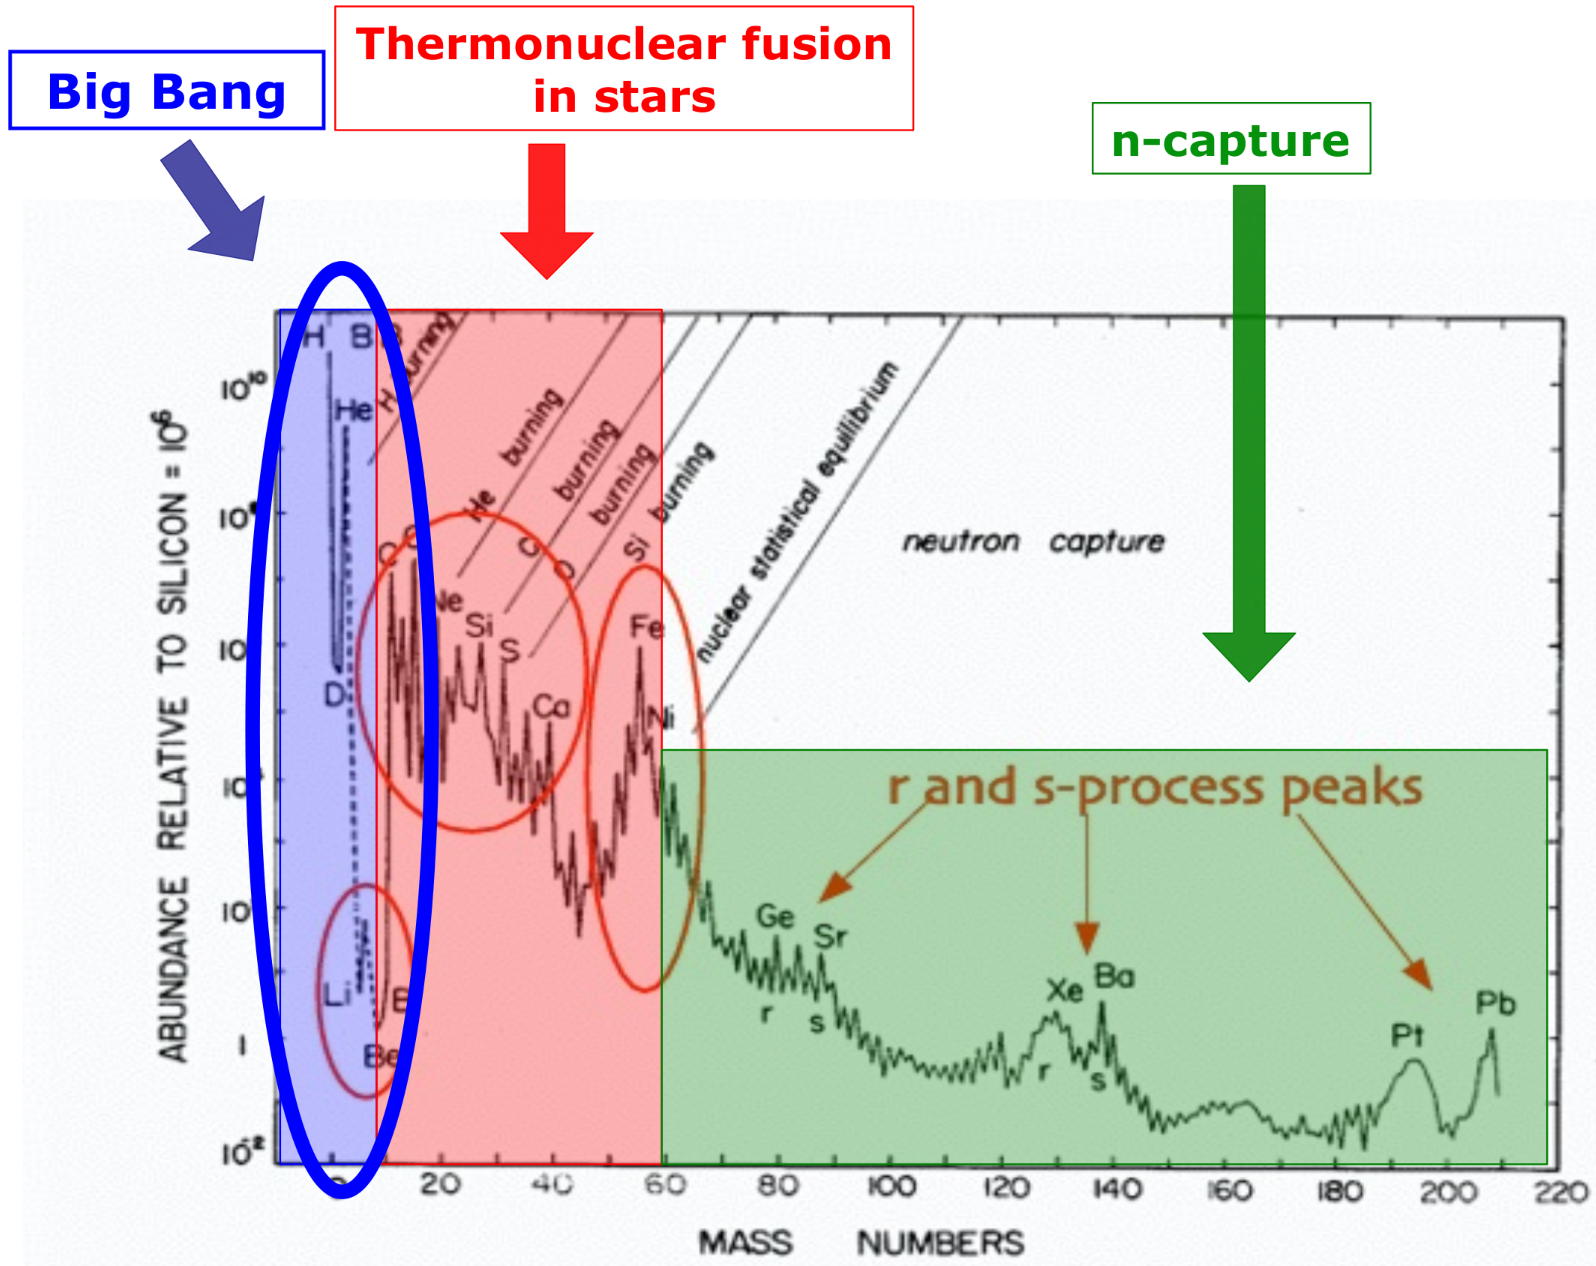
\includegraphics[width=0.5\textwidth]{immagini/processi-produzione-energia.png}
    \caption{Abbondanze degli elementi divise per i processi che li hanno generati in maniera preponderante.}
    \label{fig:processi-produzione-energia}
\end{figure}

\begin{table}
\caption{Principali reazioni nucleari.}
\label{tab:processi-produzione-energia}
\centering
\begin{tabular}{lll}
\toprule
Processo & Temperatura ($\si{K}$) & Tempo scala  ($\si{yr}$)\\
\midrule
Elementi leggeri & $\sim \SI{e6}{}$ & $\sim \SI{e5}{}$ \\
Catena PP & $\sim \SI{e7}{}$ & $\sim \SI{e10}{}$ \\
Catena CNO & $\sim \SI{e7}{}$ & $ \SI{e9}{}$\\
Catena 3--$\alpha$ & $> \SI{e8}{}$ & $\SI{e7}{}$ \\
Bruciamento carbonio & $\sim \SI{e9}{}$ & $\SI{e5}{}$ \\
Bruciamento Ossigeno & $> \SI{e9}{}$ & $\SI{e5}{}$ \\
Processo s & $> \SI{e8}{}$ & $\SI{e3}{}$--$\SI{e7}{}$ \\
Processo r & $> \SI{e10}{}$ & $\SI{10}{s}$--$\SI{100}{s}$ \\
\bottomrule
\end{tabular}
\end{table}

Essa può essere stimata così:
\begin{equation}
    \epsilon = \sum_{i=1}^{N_r} E_r \dfrac{N_r}{\si{g.s}} = \sum_{i=1}^{N_r} E_r \dfrac{N_r}{\si{cm^3.s}} \dfrac{\si{cm^3}}{\si{g}}
\end{equation}
dove con $i \in [N_r]$ si sta sommando sulle varie reazioni della catena in considerazione, $E_r$ è l'energia prodotta da ciascuna reazione, $N_r/\si{cm^3.s}$ è il numero di reazioni per unità di volume e di tempo e $\si{cm^3} / \si{g}$ rappresenta l'inverso della densità della materia stellare. Essa dipende da:
\begin{itemize}
    \item Carburante disponibile
    \item Temperatura (le reazioni si innescano dopo una certa soglia)
    \item Densità
\end{itemize}

In un modello stellare si esprime $\epsilon$ in maniera approssimata, in base alle proprietà macroscopica della struttura. In particolare possiamo scrivere:
\begin{subequations}
\label{eq:energia-reazioni-termonucleari}
\begin{align}
\epsilon_\textup{PP} &= \epsilon_1 \rho X^2 {T_6}^{\nu_\textup{PP}} \qquad \qquad \nu_\textup{PP} \in [3.5 - 6] \label{eq:energia-PP}\\
\epsilon_\textup{CN} &= \epsilon_2 \rho X X_\textup{CN} {T_6}^{\nu_\textup{CN}} \qquad \nu_\textup{CN} \in [13 - 20] \label{eq:energia-CN}\\
\epsilon_{3\alpha} &= \epsilon_3 \rho^2 Y^3 {T_8}^{\nu_{3\alpha}} \qquad \qquad \nu_{3 \alpha} \in [20 - 30] \label{eq:energia-3A}
\end{align}
\end{subequations}
dove $T_6$ significa che la temperatura è espressa in unità di $\SI{e6}{K}$, mentre $T_8$ significa che la temperatura è espressa in unità di $\SI{e8}{K}$. $X$ è l'abbondanza dell'idrogeno, $Y$ l'abbondanza dell'elio e $X_\textup{CN}$ l'abbondanza di carbonio e azoto. Si noti la mostruosa dipendenza dalla temperatura delle~\eqref{eq:energia-reazioni-termonucleari}, il che evidenzia che reazioni termonucleari stabili possono avvenire solamente in ambienti termonucleari, ovvero in cui il gas può essere considerato perfetto. Infatti, in ambienti degeneri, in cui la pressione non dipende dalla temperatura, siccome piccole variazioni di energia producono una variazione enorme della creazione di energia, la struttura può esplodere. Come si può notare, queste sono le espressioni che compaiono nell'equazione~\eqref{eq:reazioni-termonucleari}. 

\section{Riassunto sul modello stellare.}
Con le 7 equazioni presentate nel par.~\ref{sec:modelli-stellari} abbiamo un sistema di 7 equazioni in 7 incognite per descrivere la struttura di una stella. In particolare, le incognite sono:
\begin{itemize}
    \item La pressione $P$
    \item La massa $M$
    \item La densità $\rho$
    \item La luminosità $L$
    \item L'opacitk $\kappa$
    \item Il tasso di produzione di energia $\epsilon$
\end{itemize}
Queste equazioni descrivono l'interno stellare di una stella , dandomi in output la sua \emph{luminosità}. L'altro parametro di cui ho bisogno è la \emph{temperatura superficiale} della stella. Per ottenerla ho bisogno di un modello della sua atmosfera.

\chapterimage{cover/head5.png}
\chapter{Modello di atmosfera stellare}
\section{Profondità ottica}\label{sec:profondità-ottica}
Per realizzare un modello dell'atmosfera stellare si procede in maniera simile alla modellizzazione dell'interno stellare. Tuttavia, come variabile, invece della distanza dal centro, $r$, si utilizza la \emph{profondità ottica}. Infatti, le distanze dal centro sono molto elevate, pertanto è conveniente avere una misura della distanza dalla superficie della stella. 

\subsection{Profondità ottica verticale}
La profondità ottica è definita nella seguente maniera:
\begin{equation}\label{eq:profondità-ottica-atmosfera}
    \tau_\lambda = \int \kappa_\lambda \rho \ud S
\end{equation}
dove $\kappa$ è l'opacità, misurata in $\si{cm^2.g^{-1}}$, $\rho$ è la densità di massa, misurata in $\si{g.cm^{-3}}$ e $S$ rappresenta la distanza lungo una direzione radiale, misurata in $\si{cm}$.



In particolare, $\tau_\lambda = 0$ sulla superficie della stella, mentre $\tau_\lambda$ cresce andando verso il centro, seguendo un cammino radiale. Come si può notare in fig.~\ref{fig:profondita-ottica-atmosfera}, la profondità ottica \emph{non} è una misura \emph{unica} della distanza dalla superficie, infatti, se considero raggi con direzioni diverse, ottengo profondità ottiche diverse. Per utilizzare questa grandezza per misurare univocamente le distanze, si considera la \emph{profondità ottica verticale}, dove integro lungo una direzione radiale:
\begin{equation}\label{eq:profondità-ottica-verticale}
    \tau_{\lambda, V} = \int_z^0 \kappa_\lambda \rho \ud z
\end{equation}
dove la direzione identificata da $z$ è perpendicolare alla superficie della stella. A questo punto possiamo utilizzare la profondità ottica per determinare quale è lo strato più interno dal quale la radiazione a una data lunghezza d'onda riesce ad emergere verso l’esterno, o, in altre parole, la profondità ottica mi dice quanto è schermata la radiazione che viene dall'interno. D'ora in poi, quando si parlerà di profondità ottica si farà riferimento alla profondità ottica verticale.

\begin{figure}
    \centering
    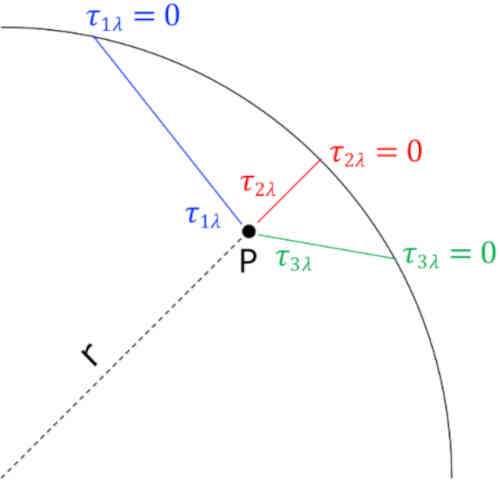
\includegraphics[width=0.3\textwidth]{immagini/profondita-ottica-atmosfera.jpg}
    \caption{La profondità ottica non è una misura univoca della distanza dalla superficie. Se scelgo tre direzioni radiali, in blu, rosso e verde, ottengo prodondità ottiche diverse in uno stesso punto P, in particolare $\tau_{1\lambda} \neq \tau_{2\lambda} \neq \tau_{3\lambda}$. L'unica cosa uguale per le tre situazioni è che in superficie la profondità ottica è nulla.}
    \label{fig:profondita-ottica-atmosfera}
\end{figure}

\subsection{Temperatura effettiva}
Sia la profondità ottica che la temperatura aumentano andando verso il centro della struttura stellare. La loro relazione definisce univocamente la così detta \emph{temperatura effettiva} della stella, ed è un'equazione chiave per un modello di atmosfera:
\begin{equation}\label{temperatura-effettiva}
    T^4 = \frac{3}{4} {T_e}^4 \bigl( \tau_\nu + \frac{2}{3} \bigr)
\end{equation}
La temperatura effettiva $T_e$ è la temperatura alla quale la profondità ottica vale $\tau_\lambda = 2 / 3$. Posso interpretare lo strato in cui ciò è vero come lo strato più interno da cui riesce ad emergere la radiazione. Per il sole, ad esempio, si ha $T_e = \SI{5770}{K}$.


\section{Righe Spettrali}\label{sec:righe-spettrali}

\subsection{Opacità per l'atmosfera stellare}\label{sec:opacita-atmosfera}
Un parametro importante per la determinazione di un modello per l'atmosfera stellare è l'opacità, già discussa nel par.~\ref{sec:opacità}. Ripassiamo i concetti principali. I processi che determinano l'opacità di una struttura sono:
\begin{description}
    \item[BB] discusso nel par.~\ref{sec:bound-bound}. Avviene a una determinata lunghezza d'onda, secondo l'eq.~\eqref{eq:lunghezza-BB}. È responsabile delle \emph{righe di assorbimento}, poiché determinano la mancanza di flusso a una determinata lunghezza d'onda.
    \item[BF] discusso nel par.~\ref{sec:bound-free}. Contribuisce all'opacità del \emph{continuo}.
    \item[FF] discusso nel par.~\ref{sec:free-free}. Contribuisce all'opacità del \emph{continuo}.
    \item[E] discusso nel par.~\ref{sec:electron-scattering}. Contribuisce all'opacità del \emph{continuo}.
\end{description}
In particolare, nelle atmosfere le temperature sono sufficientemente basse affinché i fotoni possano essere poco energetici e possano eccitare gli elettroni degli atomi, lasciandoli in stati legati. Dunque il fenomeno del BB, che negli interni stellari trascuravamo a causa delle elevate temperatura, sarà determinante nelle atmosfere. La velocità di variazione dell'opacità con la lunghezza d'onda determina come l'opacità stessa si manifesta, ovvero in forma di righe di assorbimento o nel continuo. Vediamo degli esempi.

\paragraph{Esempio--Serie di Balmer}
\paragraph{Esempio--Balmer Jump}

\subsection{Continuo spettrale e righe spettrali di assorbimento}

\subsection{Classificazione spettrale delle stelle}
Come visto nel par.~\ref{sec:opacita-atmosfera}, l'\emph{atmosfera} stellare è dove si formano il \emph{continuo spettrale} e le \emph{righe spettrali di assorbimento}. Le righe di assorbimento, in particolare, sono degli osservabili fondamentali perché è dalla loro intensità che possiamo misurare l'\emph{abbondanza} dei diversi elementi chimici. Si faccia attenzione al seguente fatto: la presenza o meno di una data riga spettrale \emph{non} dipende dalla presenza o meno di quel dato elemento, ma è fortemente modulata dalla \emph{temperatura}. Vediamo di chiarire il fatto.

Ovviamente, se un elemento non è presente nella struttura stellare, lo spettro non potrà mostrare le sue righe. Tuttavia, l'assenza di righe di un dato elemento \emph{non necessariamente} significa che quel dato elemento è assente: potrebbe esserci, ma la \emph{temperatura} non è tale da far manifestare le sue righe. Infatti, le righe di assorbimento sono dovute a fenomeni di eccitazioni o ionizzazioni della materia e, come noto,  il numero di stati eccitati o ionizzati dipende primariamente dalla temperatura. Se, ad esempio, la temperatura non è sufficientemente alta da far sì che tutti gli atomi di un dato elemento siano ionizzati, non potrò mai vedere la riga di assorbimento di tale elemento, anche se esso è presente.

In definitiva, è la temperatura che modula il manifestarsi delle righe spettrali, ovvero è la \emph{temperatura} che determina il \emph{tipo spettrale} delle stelle. Dunque, le stelle sono classificate in base al loro tipo spettrale, ovvero in base alla presenza e all'intensità delle varie righe spettrali, il quale, a sua volta, riflette il valore della temperatura atmosferica della stella.

\begin{figure}
    \centering
    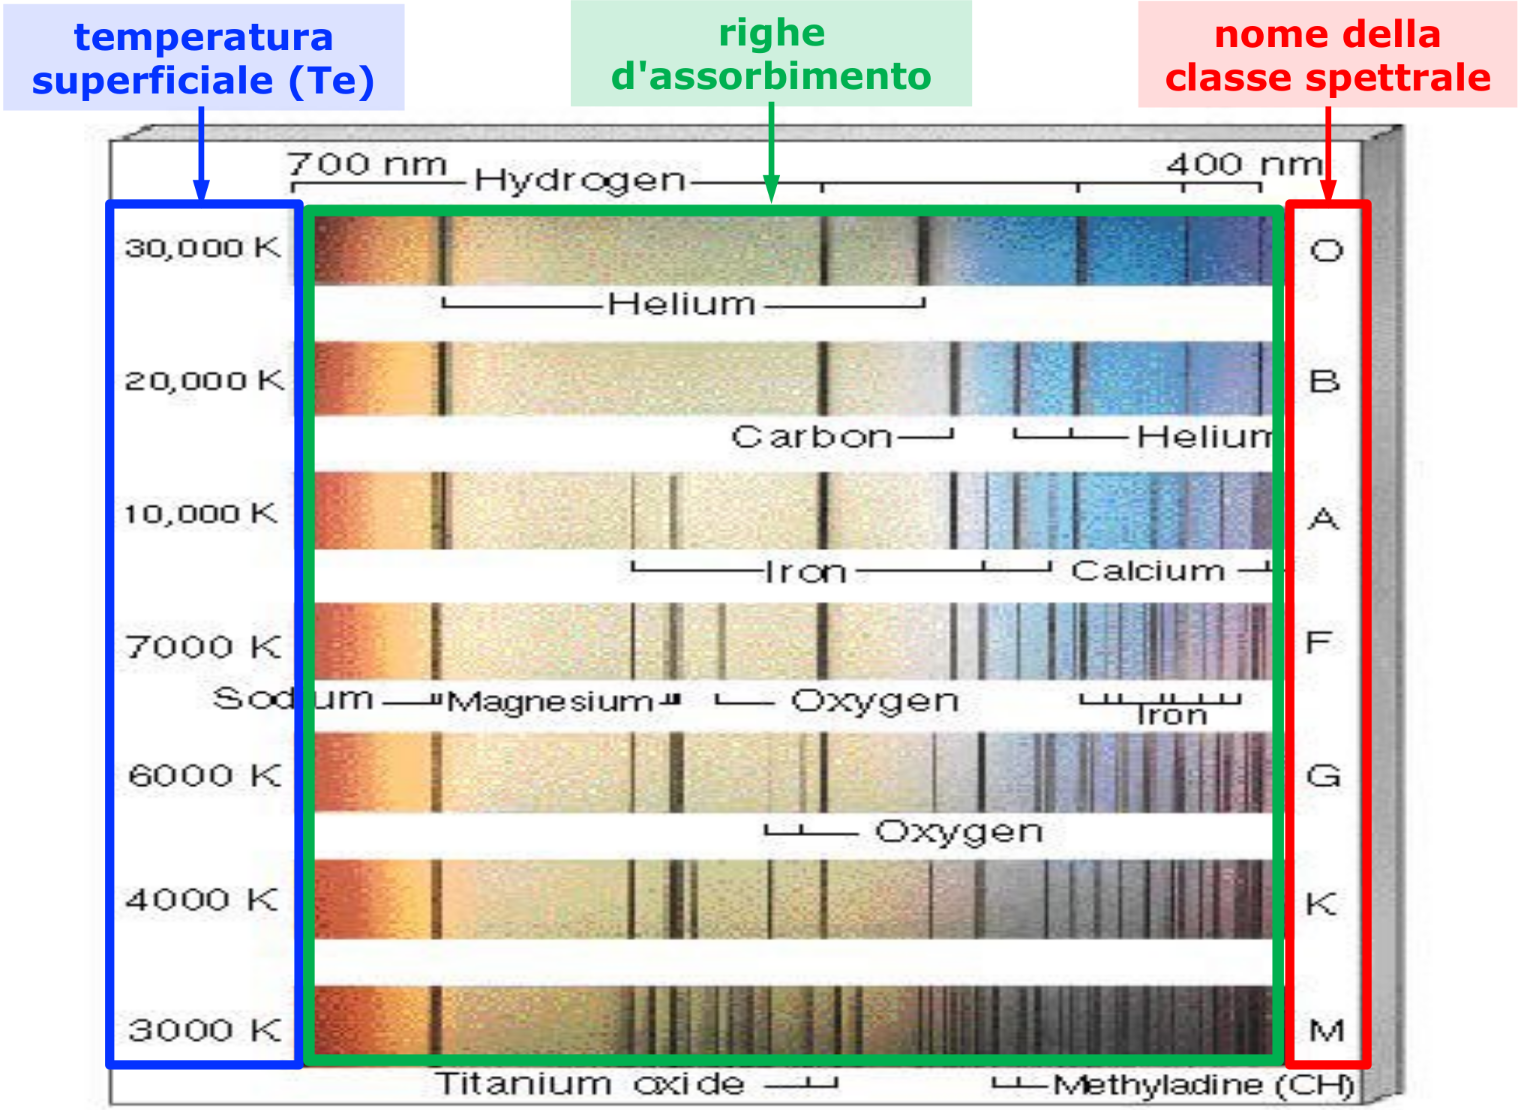
\includegraphics[width=0.6\textwidth]{immagini/classificazione-spettrale-stelle.png}
    \caption{Classi spettrali principali.}
    \label{fig:classificazione-spettrale-stelle}
\end{figure}

\begin{figure}
    \centering
    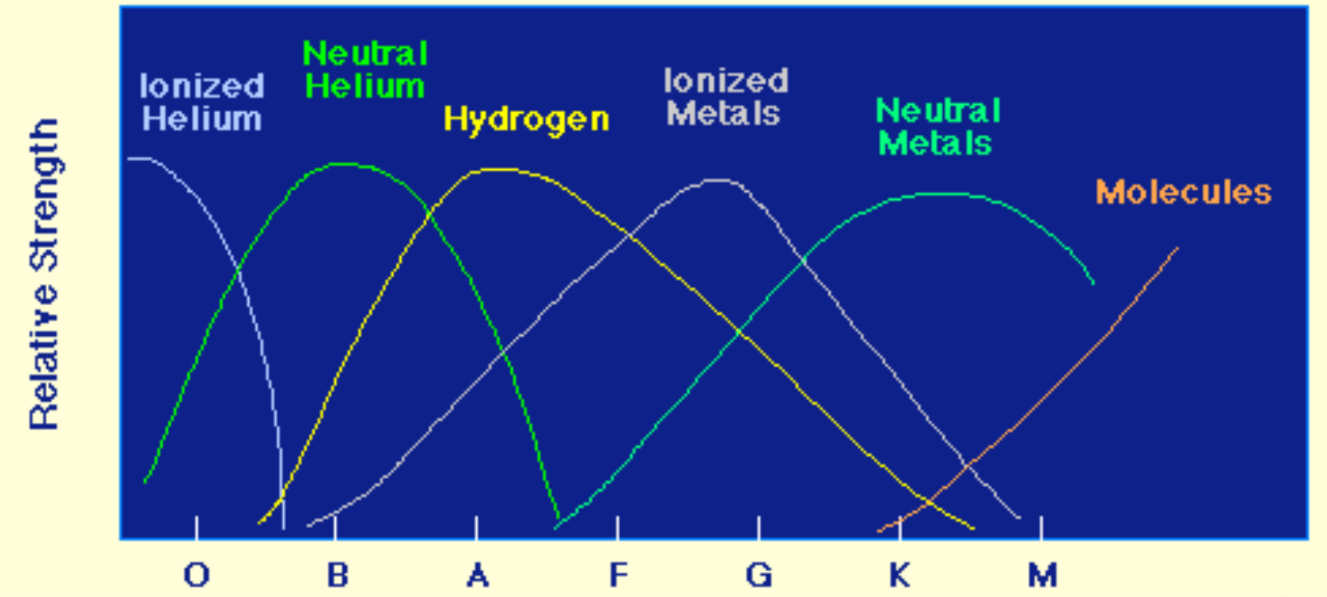
\includegraphics[width=0.6\textwidth]{immagini/classificazione-spettrale-stelle-2.png}
    \caption{Classi spettrali principali.}
    \label{fig:classificazione-spettrale-stelle-2}
    
\end{figure}

Nelle fig.~\ref{fig:classificazione-spettrale-stelle} e fig.~\ref{fig:classificazione-spettrale-stelle-2} sono rappresentate le principali \emph{classi spettrali}, elencate anche di seguito:
\begin{description}
    \item[O] $T_e > \SI{25000}{K}$
    \item[B] $ \SI{11000}{K} < T_e < \SI{25000}{K}$: ???
    \item[A] $ \SI{7500}{K} < T_e < \SI{11000}{K} $: ???
    \item[F] $ \SI{6000}{K} < T_e < \SI{7500}{K} $: ???
    \item[G] $ \SI{5000}{K} < T_e < \SI{6000}{K} $: ???
    \item[K] $ \SI{3500}{K} < T_e < \SI{3000}{K} $: ???
    \item[M] $ \SI{3500}{K} < T_e < \SI{3000}{K} $: ???
\end{description}
Si può ricordare tale lista con la seguente frase: \emph{"O,B,A, Fine Girl Kiss Me"}.

Come detto precedentemente, una data riga di assorbimento è presente o assente nello spettro a seconda del numero di atomi nei diversi stati eccitati o ionizzati di quel dato elemento. Tale numero dipende in primo luogo dalla temperatura e viene stimato attraverso:
\begin{description}
    \item[Equazione di Boltzmann]: percentuale di atomi in un dato stato di eccitazione. Risponde alla domanda: "quale frazione di atomi con elettroni legati si trova in un dato stato eccitato?"
    \item[Equazione di Saha]: percentuale di atomi in un dato stato di ionizzazione. Risponde alla domanda: "questo elemento ha ancora elettroni legati?"
\end{description}

\subsection{Equazione di Boltzmann}\label{sec:equazione-boltzmann}
Come suggerito nel precedente paragrafo, l'\emph{equazione di Boltzmann} fornisce la percenutale di atomi in un dato stato di eccitazione. In particolare, per ogni specie chimica, considera gli atomi ionizzati $j$--volte ($N_j$) e fornisce la frazioen di quelli che sono eccitati $i$--volte ($N_{ji}$):
\begin{equation}\label{eq:equazione-boltzmann}
    \dfrac{N_{ji}}{N_j} = \dfrac{g_i}{{U_j}(T)} 10^{-\theta \chi_i} 
\end{equation}
dove:
\begin{description}
    \item[$N_j$]: numero di atomi nello stato di ionizzazioni j (ovvero ionizzati $j$--volte).
    \item[$N_{ji}$]: numero di atomi nello stato di ionizzazione j, che si trovano nello stato di eccitazioni i (ovvero ionizzati $j$--volte \emph{ed} eccitati $i$--volte).
    \item[$g_i$]: peso statistico del livello energetico i.
    \item[$\theta \equiv \frac{5040}{T} \si{eV^{-1}}$], con $T$ espressa in $\si{K}$.
    \item[${U_j}(T)$]: funzione di partizione per lo stato di ionizzazione j.
    \item[$\chi_i$]: potenziale di eccitazione dal primo livello energetico disponibile al livello energetico $i$.      
\end{description}
Notiamo che l'espressione è dipendente dalla struttura dell'atomo, attraverso i termini $g_i$, ${U_j}(T)$ e $\chi_i$, e dalla temperatura. In definitiva, la percentuale è tanto maggiore quanto più alta è $T$ e quanto più basso è il potenziale di eccitazione $\chi_i$. Vediamo, ora, i vari termini con maggior dettaglio.

\paragraph{Peso statistico}
Il peso statistico $g_i$ del livello energetico $i$--esimo rappresenta il numero di livelli energetici degeneri, ovvero alla stessa energia. Per gli atomi idrogenoidi si ha:
\begin{equation*}
g_i = 2 i^2
\end{equation*}
e si ottengono i noti risultati per cui il nel livello fondamentale ($i=1$) si ha $g_1 = 2$, ovvero possono alloggiare $2$ elettroni di spin opposto, mentre nel primo livello eccitato, $i=2$, vale $g_2=8$ e possono alloggiare $2$ elettroni nell'orbitale s e $6$ elettroni nell'orbitale p, e così via.

\paragraph{Funzione di partizione}
La funzione di partizione per lo stato di ionizzazione $j$--esimo, ${U_j}(T)$, è una sommatoria dei pesi statistici ($g_i$) di tutti i livelli energetici pesati con un termine che dipende dalla temperatura, ovvero:
\begin{equation*}
    {U_j}(T) = \sum_i g_i 10^{-\theta \chi_i}
\end{equation*}

\paragraph{Potenziale di eccitazione}
nell'equazione~\eqref{eq:equazione-boltzmann}, $\chi_i$ rappresenta il potenziale di eccitazione dal primo livello energetico \emph{disponibile} al livello energetico $i$--esimo. Vediamo cosa si intende per primo livello disponibile, il quale dipenderà dal livello di ionizzazione, j. Consideriamo, ad esempio, \ce{NeI}, ovvero il neon neutro. Esso ha 10\ce{e^-} legati, in cui $2$\ce{e^-} si trovano nel livello $n=2$ e $8$\ce{e^-} si trovano nel livello $n=2$. Essendo, dunque, i primi due livelli totalmente occupati, il primo livello disponibile sarà $n=3$. Nel caso di \ce{NeII}, ovvero del neon ionizzato $1$ volta, il primo livello disponibile è $n=2$, non essendo questa volta occupato del tutto. 

Per gli atomi idrogenoidi, il potenziale di eccitazione tra due livelli energetici $a$ e $b$, con $a<b$, è:
\[
    \chi_{ab} = Z^2 \bigl( \dfrac{1}{{n_a}^2} - \dfrac{1}{{n_b}^2} \bigr) \times \SI{13.6}{eV}
\]
con $Z$ il numero atomico. Essendo il primo livello energetico disponibile il livello fondamentale, rappresentato da $a=1$, si ha:
\[
  \chi_i = Z^2 \bigl( 1-\dfrac{1}{i^2}  \bigr)  \times \SI{13.6}{eV}
\]

\subsection{Equazione di Saha}\label{sec:equazione-saha}
Per ogni specie chimica, l'\emph{equazione di Saha} fornisce la percentuale di atomi ionizzati $j+1$--volte ($N_{j+1}$) rispetto al numero di atomi ionizzati $j$--volte ($N_j$):
\begin{equation}\label{eq:equazione-saha}
    \log \dfrac{N_{j+1}}{N_j} = -0.176 - \log P_e - \theta \chi_i + 2.5 \log T + \log \dfrac{{U_{j+1}}(T)}{{U_j}(T)}
\end{equation}
dove:
\begin{description}
    \item[$N_j$, $N_{j+1}$]: numero di atomi nello stato di ionizzazione $j$ e $j+1$, ovvero contigui.
    \item[$P_e$]: pressione elettronica, ovvero esercitata dalla componente elettronica del gas. Si ricordi che siamo nelle atmosfere stellari, in cui il gas è sempre approssimabile come gas perfetto.
    \item[$\theta \equiv \frac{5040}{T} \si{eV^{-1}}$], con $T$ espressa in $\si{K}$.
    \item[$\chi_i$]: potenziale di ionizzazione dell'atomo ionizzato $j$--volte. ERRORE FORSE, NON DOVREBBE ESSERE CHI J??????
    \item[${U_j}(T)$, ${U_{j+1}}(T)$]: funzioni di partizione per gli stati di ionizzazione $j$ e $j+1$.
\end{description}
Si faccia molta attenzione a cosa si riferisce l'eq.~\eqref{eq:equazione-saha}. Essa \emph{non} permette di calcolare il numero di atomi in un certo stato di ionizzazione ( $N_j$ ) rispetto al numero totale ($N$) di atomi di quella specie, che sarebbe equivalente a $N_j / N$, tuttavia essa calcola il rapporto tra il numero di atomi in due stati di ionizzaione contigui ($j+1$ e $j$), equivalente a $N_{j+1} / N_j$. Per ottenere $N_j / N$ sono necessarie applicazioni successive dell'equazione di Saha tra due stati di ionizzazione contigui.

\subsection{Frazione di atomi attivi}\label{sec:frazione-atomi-attivi}
In pratica, mettendo insieme le due equazioni, per ogni equazione chimica:
\begin{itemize}
    \item l'equazione di Saha~\eqref{eq:equazione-saha} mi dice se, a quella data temperatura $T$ esistono atomi che non sono completamente ionizzati, cioè che hanno ancora elettroni legati
    \item se ciò è vero, l'equazione di Boltzmann~\eqref{eq:equazione-boltzmann} mi dice se, a quella data temperatura $T$ gli elettorni legati sono nello stato fondamentale o in quale livello di eccitazione
\end{itemize}
Insieme, le eq.~\eqref{eq:equazione-saha} e~\eqref{eq:equazione-boltzmann} forniscono la \emph{frazione di atomi attivi} $N_a$ (che generano le righe spettrali) rispetto al totale di atomi di quella specie. È possibile misurare $N_a$ attraverso un'analisi spettroscopica delle righe spettrali, dunque, in definitiva, usando le equazioni di Saha e Boltzmann è possibile ricavare l'\emph{abbondanza} di quel dato elemento chimico. 

\subsection{Analisi delle righe spettrali}
Come discusso nel par.~\ref{sec:opacita-atmosfera}, le linee spettrali sono originate dalle transizioni elettroni che di tipo bound--bound. Nelle righe spettrali sono contenute informazioni di cruciale importanza, tra cui le \emph{abbondanze chimiche} e la \emph{velocità radiale}.

\begin{figure}
    \centering
    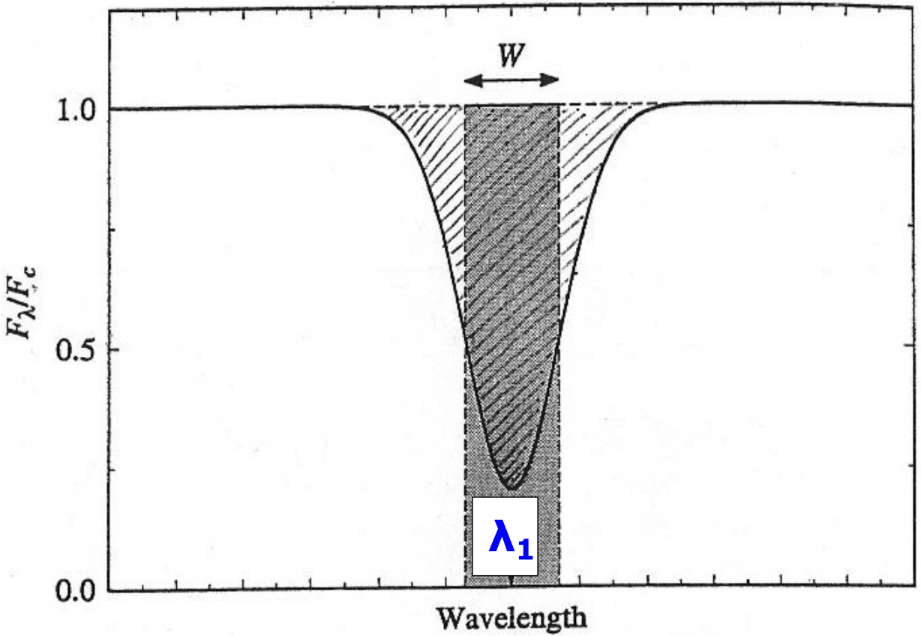
\includegraphics[width=0.5\textwidth]{immagini/righe-spettrali.png}
    \caption{Misura di una riga spettrale e analisi per la determinazione della velocità radiale e delle abbondanze chimiche. La riga spettrale di una transizione elettronica B--B è misurata a lunghezza d'onda $\lambda_1$, confrontata con la lunghezza d'onda di laboratorio di tale transizione $\lambda_0$.}
    \label{fig:righe-spettrali}
    
\end{figure}

Per capire come si procede sperimentalmente all'analisi delle righe spettrali, consideriamo una situazione tipo, illustrata in fig.~\ref{fig:righe-spettrali}. Immaginiamo di misurare una riga spettrale corrispondente a una data transizione elettronica a una lunghezza d'onda $\lambda_1$, diversa, in generale, dalla lunghezza d'onda di laboratorio di tale transizione, $\lambda_0$. A causa dell'\emph{effetto Doppler}, la differenza tra la lunghezza d'onda misurata e quella di laboratorio è una misura diretta della \emph{velocità radiale} della stella. Infatti si ha:
\begin{equation}\label{eq:effetto-doppler}
    \dfrac{\lambda_1 - \lambda_0}{\lambda_0} = \dfrac{\Delta \lambda}{\lambda_0} = \dfrac{v_r}{c}
\end{equation}

Per ciò che concerne le \emph{abbondanze chimiche}, è necessario misurare l'\emph{intensità} delle righe spettrali prodotte dagli atomi della specie studiata attraverso transizioni BB. In particolare, l'intensità, come mostrato in fig.~\ref{fig:righe-spettrali}, è rappresentata dall'area sotto la curva dello spettro continuo. È tuttavia comunemente misurata in termini di \emph{larghezza equivalente}. La larghezza equivalente $W$ è la larghezza (in Armstrong) di un rettangolo di altezza unitaria e area uguale all'intensità della riga spettrale. Si può calcolare nella seguente maniera:
\begin{equation}\label{eq:larghezza-equivalente}
    W = \int \dfrac{F_c - F_\lambda}{F_c} \ud \lambda
\end{equation} 
dove $F$ rappresenta il flusso. In particolare $W$ è correlato con il numero di atomi per $\si{cm^2}$ che generano la transizione, ovvero con $N_a$, il numero di atomi attivi. Come è possibile osservare in figura~\ref{fig:larghezza-equivalente}, la riga spettrale è tanto più profonda quanto maggiore è l'abbondanza dell'elemento considerato. Siccome la profondità della riga dipende dal numero di atomi attivi, anche $W$ dipenderà da $N_a$. In particolare è possibile osservare la loro correlazione in una \emph{curva di crescita}, mostrata in fig.~\ref{fig:curva-crescita}. Come si osserva dal grafico, l'andamento di $W$ con $N_a$ varia all'aumentare del numero di atomi attivi. Nel \emph{regime lineare} si ha $W \propto N_a$ poiché $W$ è dominata dal contributo del core della riga, evidenziato nella fig.~\ref{fig:larghezza-equivalente-regime-lineare}. Aumentando il numero di atomi attivi si entra nel \emph{regime piatto (o di saturazione)}, in cui si ha $W \propto \sqrt{\log N_a}$. In questo regime $W$ cresce molto lentamente, poiché il core della riga è saturo (la riga ha massima profondità, ovvero arriva a toccare lo zero) e il contributo delle ali è ancora trascurabile, come mostrato in fig.~\ref{fig:larghezza-equivalente-regime-piatto}. Nel \emph{regime di smorzamento} $W$ si ha $W \propto \sqrt{N_a}$ e $W$ torna ad essere più sensibile alle variazioni di $N_a$ rispetto al regime di saturazione, poiché le ali hanno un contributo dominante, come mostrato in fig.~\ref{fig:larghezza-equivalente-regime-smorzamento}.

\begin{figure}
    \centering
    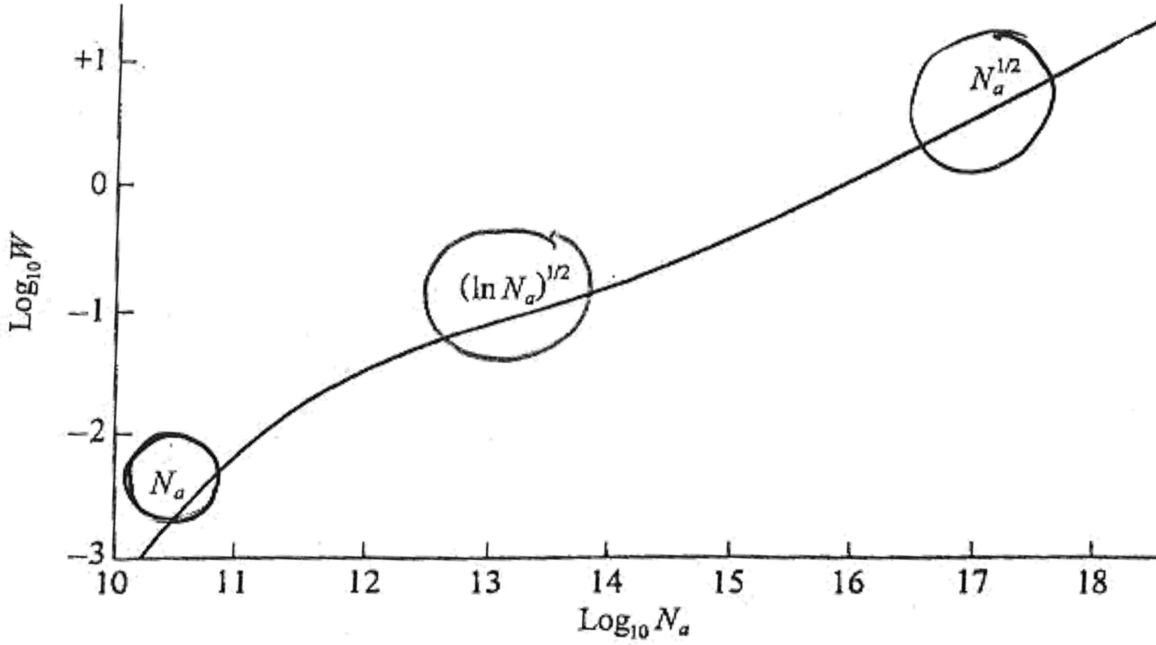
\includegraphics[width=0.5\textwidth]{immagini/curva-crescita.png}
    \caption{Curva di crescita. Descrive la dipendenza della larghezza equivalente $W$ dal numero di atomi attivi $N_a$. La curva è doppio--logaritmica. L'andamento varia con l'aumentare degli atomi attivi. In particolare, sono presenti tre regimi: il regime lineare in cui $W \propto N_a$, il regime piatto in cui $W \propto \sqrt{\log N_a}$ e il regime di smorzamento in cui $W \propto \sqrt{N_a}$.} 
    \label{fig:curva-crescita}
\end{figure}

\begin{figure}
\centering
\subfloat[][\emph{Regime lineare}\label{fig:larghezza-equivalente-regime-lineare}]
    {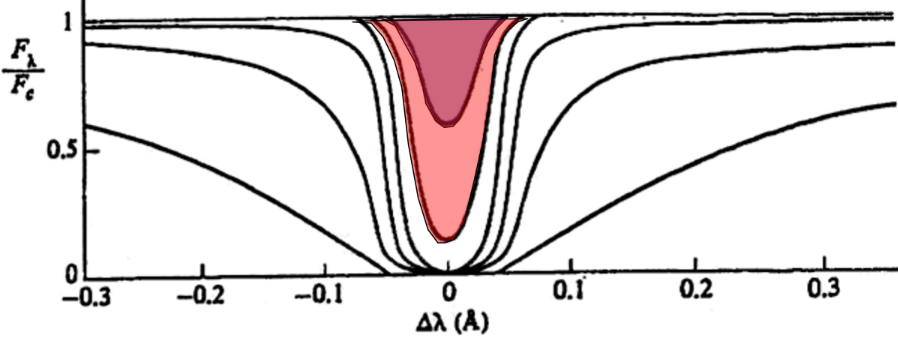
\includegraphics[width=0.45\textwidth]{immagini/larghezza-equivalente-regime-lineare.png}} \quad
\subfloat[][\emph{Regime piatto o di saturazione}\label{fig:larghezza-equivalente-regime-piatto}]
    {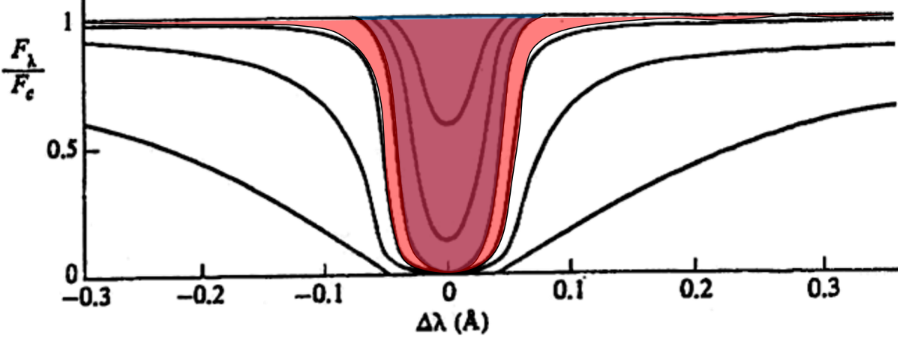
\includegraphics[width=0.45\textwidth]{immagini/larghezza-equivalente-regime-piatto.png}} \quad
\subfloat[][\emph{Regime di smorzamento}\label{fig:larghezza-equivalente-regime-smorzamento}]
    {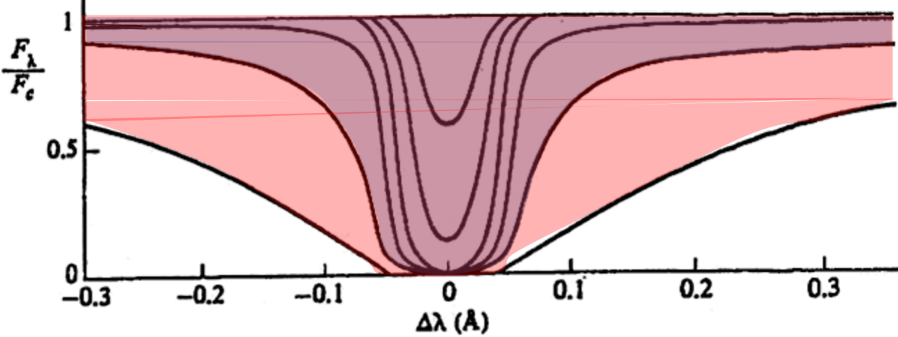
\includegraphics[width=0.45\textwidth]{immagini/larghezza-equivalente-regime-smorzamento.png}}
\caption{Correlazione tra la larghezza equivalente $W$ e il numero di atomi attivi $N_a$. La riga spettrale è tanto più profonda quanto maggiore è l’abbondanza dell’elemento considerato.}
\label{fig:larghezza-equivalente}
\end{figure}

Conoscendo la curva di crescita è possibile ricavare il numero di atomi attivi data la larghezza equivalente, che a sua volta può essere ricavata sperimentalmente dall'analisi spettroscopica del corpo in esame. Tuttavia, siamo interessati all'\emph{abbondanza} di un elemento, piuttosto che il numero dei suoi atomi attivi, $N_a$, che dipende sensibilmente dalla temperatura dell'atmosfera stellare. Ovviamente il numero totale di atomi di una data specie, $N_\textup{tot}$, \emph{non} dipende dalla temperatura. Per ottnere $N_\textup{tot}$ dalla misura di $N_a$ è necessario conoscere la percetuale di atomi di quella data specie chimica che sono nella condizione di attivare le transizioni elettroniche che generano la linea di assorbimento che si sta misurando. Abbiamo dunque bisogno di conoscere:
\begin{enumerate}
    \item la percentuale di atomi che hanno ancora elettroni legati alla struttura atomica alla data temperatura $T$, ovvero il \emph{fattore di ionizzazione}. Esso si trova con l'\emph{equazione di Boltzmann}~\eqref{eq:equazione-boltzmann} (vedi par.~\ref{sec:equazione-boltzmann}).
    \item la percentuale di atomi nei quali gli elettroni possono effettuare le transizioni osservata alla data temperatura $T$, ovvero il \emph{fattore di eccitazione}. Esso si trova con l'\emph{equazione di Saha}~\eqref{eq:equazione-saha} (vedi par.~\ref{sec:equazione-saha}).
\end{enumerate} 

A questo punto, conoscendo il numero totale di atomi di un dato elemento, $N_\textup{tot}$, è possibile trovare l'abbondanza in massa di tale elemento nell'atmosfera stellare:
\begin{equation}\label{eq:abbondanza-in-massa}
    A_\textup{el} = N_\textup{tot} m_\textup{el}
\end{equation}
dove $N_\textup{tot}$ è il numero di atomi per \si{cm} quadro, ovvero è espresso in \si{cm^{-2}}, $m_\textup{el}$ è la massa dell'elemento, espressa in \si{g} e $A_\textup{el}$ è misurato in \si{g.cm^{-2}}. Tuttavia, si preferisce riferirsi alle \emph{square bracket abundances}.

\subsection{square bracket abundances}
Le abbondanze in massa, espresse dall'eq.~\eqref{eq:abbondanza-in-massa}, sono tipicamente normalizzate all'abbondanza di idrogeno presente nella stella studiata e anche rispetto al rapporto nel Sole, espressi in scala logaritmica. Per fare un esempio chiaritivo, supponiamo di voler esprimere l'abbondanza del sodio in una stella. Con la eq.~\eqref{eq:abbondanza-in-massa} trovo $A_\textup{Na} = \SI{9.3e-5}{g.cm^{-2}}$. Essa è normalizzata rispetto all'abbondanza dell'idrogeno nella stella stessa, che suppongiamo essere $A_\textup{H} = \SI{1.1}{g.cm^{-2}}$, in scala logaritmica:
\[
\log \Bigl( \dfrac{A_\textup{Na}}{A_\textup{H}} \Bigr)_* \sim -4 -0 = -4    
\]
A sua volta questa quantità è riferita alla quantità analoga del nostro Sole, che in questo caso vale:
\[
    \log \Bigl( \dfrac{A_\textup{Na}}{A_\textup{H}} \Bigr)_\odot = 6.33 - 12 = -5.67
\]
Ora, il logaritmo del rapporto tra l'abbondanza del sodio nell stella normalizzata rispetto all'idrogeno e l'abbondanza del sodio nel Sole normalizzata rispetto all'idrogeno ci dà la \emph{square bracket adundance} del sodio:
\[
\Bigl[ \dfrac{\textup{Na}}{\textup{H}} \Bigr] = \log \dfrac{\Bigl(\frac{A_\textup{Na}}{A_\textup{H}}\Bigr)_*}{\Bigl(\frac{A_\textup{Na}}{A_\textup{H}}\Bigr)_\odot} = \log \Bigl( \dfrac{A_\textup{Na}}{A_\textup{H}} \Bigr)_* - \log \Bigl( \dfrac{A_\textup{Na}}{A_\textup{H}} \Bigr)_\odot = -4 -(-5.67) = +1.67
\]
ovvero, nella stella osservata il sodio è $10^{1.67} \sim 50$ volte \emph{più abbondante} che nel Sole. In generale si ha la seguente formula:
\begin{equation}\label{eq:square-bracket-abundances}
    \Bigl[ \dfrac{\textup{el}}{\textup{H}} \Bigr] = \log \Bigl( \dfrac{A_\textup{el}}{A_\textup{H}} \Bigr)_* - \log \Bigl( \dfrac{A_\textup{el}}{A_\textup{H}} \Bigr)_\odot
\end{equation}
Secondo l'eq.~\eqref{eq:square-bracket-abundances}, $[\frac{el}{H}] = 0$ significa che l'abbondanza in massa dell'elemento \emph{el} è la stessa del Sole, $[\frac{el}{H}] = -0.5$ significa che è pari a $1/3$ di quella del Sole e $[\frac{el}{H}] = -2$ significa che è $1/100$ di quella del Sole.



\chapterimage{cover/head6.png}
\chapter{Evoluzione Stellare}
\section{Modello di evoluzione stellare}\label{sec:modello-evoluzione-stellare}

\subsection{Introduzione all'evoluzione stellare}
\subsection{Diagramma H--R e traccia evolutiva}

\section{Pre Main Sequence}\label{sec:pre-main-sequence}

La fase di pre-MS (pre main sequence) è quella in cui si va a formare una stella, partendo dalla contrazione di una nube di gas. Per far si che questa si formi, però, è necessario che siano presenti determinate condizioni. Sia $m$ la massa di una particella d'Idrogeno ai margini della nube gassosa (possibilmente una molecola di $H_2$) e si indichi con $R$ la distanza di questa dal centro. Al fine di osservare la formazione di una stella è necessario che l'attrazione gravitazionale agente sulla particella, dal resto della nube, sia maggiore rispetto alla pressione esercitata dal gas su di essa, imponiamo quindi l'equazione~\refeq{eq:1}
\begin{equation}
    G \frac{M m}{R} \geq k_B T
    \label{eq:1}
\end{equation}
dove $M$ è la massa della nube, $T$ è la temperatura e $k_B$ la costante di Boltzmann.
\subsection{Massa di Jeans}\label{sec:massa-jeans}

Considerando che la massa della nube può essere espressa come segue
\[
    M = \frac{4}{3} \pi R^3 \rho
\]
allora possiamo esplicitare la dipendenza del raggio da alcune caratteristiche della nube, in particolare della massa e della densità.
\begin{equation}
    R = \sqrt{\frac{3}{4\pi} \frac{M}{\rho}}
    \label{eq:2}
\end{equation}
Inserendo l'equazione~\refeq{eq:2} nella (\refeq{eq:1}), si ottiene la relazione in cui compaiono le varie caratteristiche del gas, imponendo le condizioni che permettono la formazione di una stella.
\begin{equation}
    M^{\frac{2}{3}} \geq \frac{k_B T}{G m} \sqrt{\frac{3}{4\pi} \frac{1}{\rho}}
    \label{eq:3}
\end{equation}
Sia $a = \sqrt{\frac{3}{4\pi}}\frac{k_B}{G m} \sim \SI{e16}{g.K^{-1}.cm^{-1}}$ una costante, allora si riscrive la relazione~\refeq{eq:3} nella forma dell'equazione~\refeq{eq:jeans}.
\begin{equation}
    M \geq a^{\frac{3}{2}} T^{\frac{3}{2}} \rho^{-\frac{1}{2}}
\label{eq:jeans}
\end{equation}

Questa è la massa necessaria che permette la contrazione, assumendo che la densità di gas sia uniforme e il valore minimo che soddisfa questa disuguaglianza viene detto massa di Jeans, la quale dipende dai valori di densità e temperatura del gas. In particolare, per temperature elevate e gas rarefatti questa risulta maggiore rispetto al caso con gas densi e relativamente freddi. Di conseguenza si deduce che l'ambiente più favorevole alla formazione stellare è proprio quest'ultimo.

Benché il modello costruito permette di trovare le condizioni iniziali necessarie a favorire la nascita di una stella, il meccanismo che attiva l'effettivo collasso gravitazionale non è ancora ben noto. Le ipotesi più probabili sono quelle dello Shock Front, cioè la compressione dovuta all'esplosione di una supernova, della collisione tra nubi o all'interazione con una galassia.
\subsection{Initial mass function}
Si consideri ora di essere in condizioni interstellari ($T = \SI{10}{K}$ e $ \bar \rho = \SI{e-23}{g.cm^{-2}} $), allora per formare una stella sarebbe necessaria una massa di circa $100 \;M_\odot $, ma noi osserviamo stelle anche decisamente meno massive. Questo significa che in realtà tale meccanismo favorisce la formazione di vari aggregati stellari, con processi frammentati riferiti alla nube iniziale. Definiamo ora con IMF (initial mass function) la distribuzione di massa della stella in formazione all'interno di una popolazione stellare, utile per studiare i passaggi che una data stella attraversa durante la sua evoluzione, in particolare questo valore permette di avere una stima delle seguenti grandezze:
\begin{description}
    \item[Destino]di una stella, cioè quale percorso una stella seguirà nella parte finale della sua vita;
    \item[Durata della vita]di una stella, indica l'ordine di grandezza del tempo necessario alla sua evoluzione;
    \item[Inquinamento]di una stella, ovvero i tipi di elementi chimici che essa rilascia nell'universo nelle ultime fasi della propria vita.
\end{description}

Essendo la IMF una funzione di natura empirica, le sue caratteristiche non sono ancora ben conosciute. Questo significa che non è ben chiaro quale sia la forma di tale funzione e nemmeno se valga in maniera universale. Ovvero se sia indipendente dal tempo, caratteristiche della nube o, addirittura, dalla posizione nello spazio. Un'ipotesi del suo andamento vuole che questa prenda la forma dell'equazione~\refeq{eq:IMF},
\begin{equation}
    \Psi(M) = k M^{-s}
    \label{eq:IMF}
\end{equation}
dove $s$ è un numero positivo e $k$ una costante di proporzionalità.

Si osserva che se il modello dovesse avere questa forma, allora la percentuale di stelle massicce è decisamente minore rispetto a quella di stelle con massa relativamente piccola. Tale predizione viene confermata dal fatto che la morte di una stella molto massiva produce un'implosione sul nucleo stesso generando una supernova, ma nel nostro cielo tali avvenimenti non sono così comuni. L'andamento della IMF è mostrato nella figura~\ref{fig:IMF}.

\begin{figure}
    \centering
    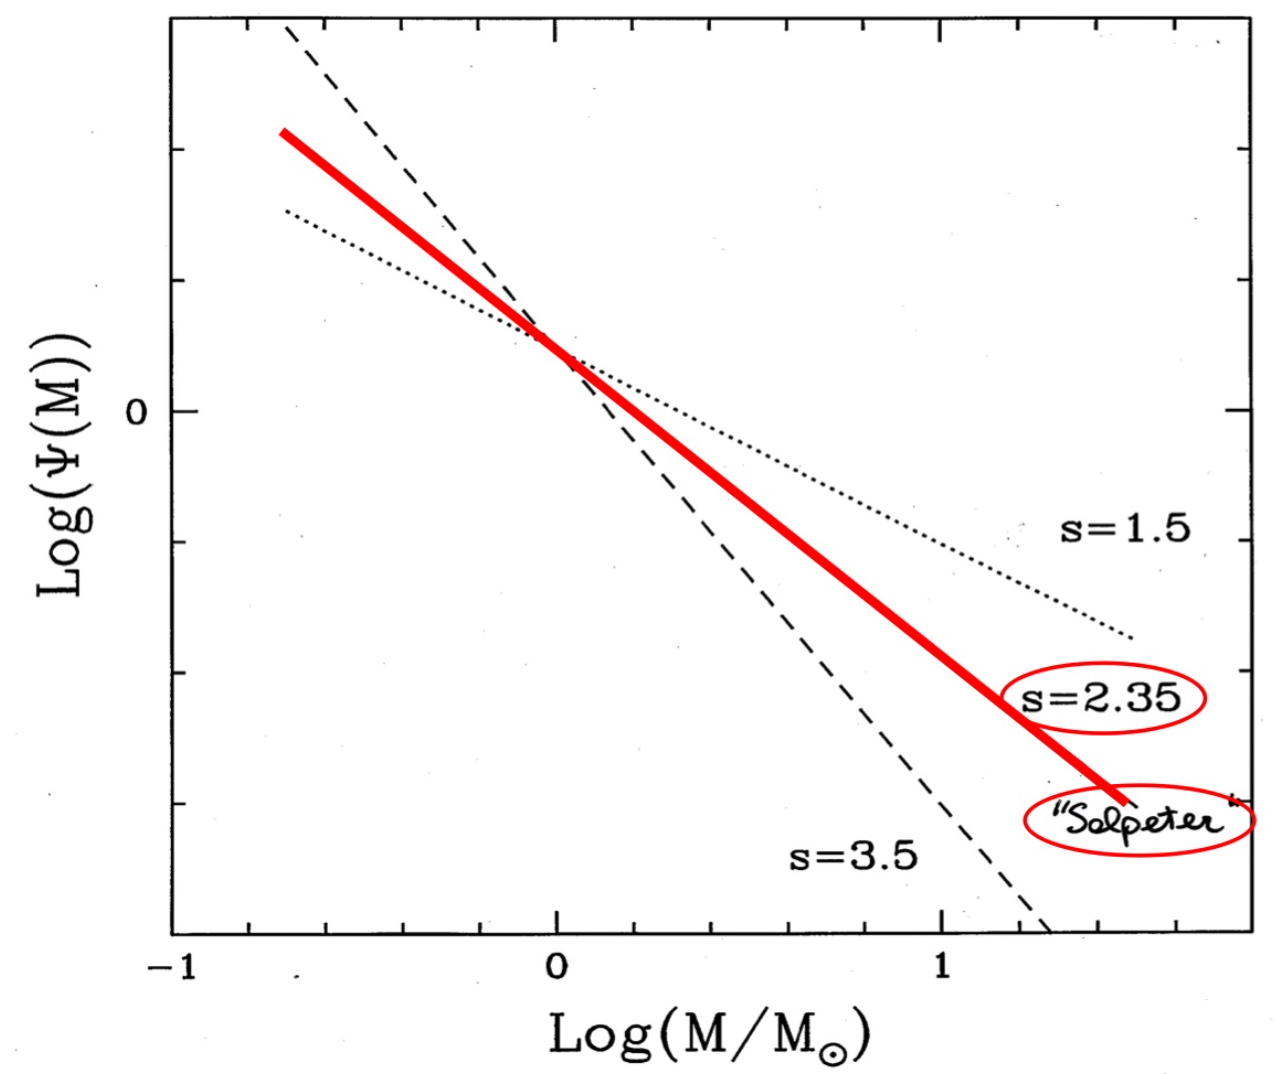
\includegraphics[width = 0.3\textwidth]{immagini/IMF.png}
    \caption{La figura mostra l'andamento della IMF in funzione della massa (normalizzata a quella solare) in scala logaritmica. La presenza di più linee è dovuta al fatto che non è presente una stima unica del parametro $s$ e di conseguenza sono indicate varie possibilità per questo parametro dove in rosso si ha quella più probabile.}\label{fig:IMF}
\end{figure}
\subsection{Protostelle e Teorema di Hayashi}

Data ora una nube di gas non uniforme, questa si inizierà a frammentare verso le varie buche di potenziale gravitazionale, in cui se la massa  soddisfa il criterio di Jeans (\refeq{eq:jeans}), allora si innescherà il collasso, producendo un oggetto che verrà definito con il termine \textit{Protostella}. Quando la contrazione innesca le reazioni termonucleari, generando un equilibrio idrostatico tra pressione gravitazionale e pressione di radiazione, la stella sarà completamente convettiva. Questo stato può essere rappresentato nel diagramma H-R come un punto della \textit{traccia di Hayashi}. Si tratta di una linea nel piano H-R che, data una stella con una determinata composizione chimica, mostra al variare della massa un punto del diagramma in cui questa è in equilibrio idrostatico e completamente convettiva. Tale curva quindi mostra una famiglia di stelle con la stessa composizione chimica, ma differente massa iniziale.

Il teorema di Hayashi afferma, inoltre, che fissata la composizione chimica e la massa di una stella, esiste una regione del piano H-R dove non è possibile realizzare modelli stellari in equilibrio idrostatico, la cui traccia di Hayashi funge da bordo. In figura~\ref{fig:hay} è mostrata la zona in questione colorata in rosso, mentre in verde si ha la regione che permette di avere modelli stabili, parzialmente convettivi. La validità di questo teorema è generale,  continua quindi a valere per ogni punto dell'evoluzione stellare, in modelli convettivi e non.

\begin{figure}
    \centering
    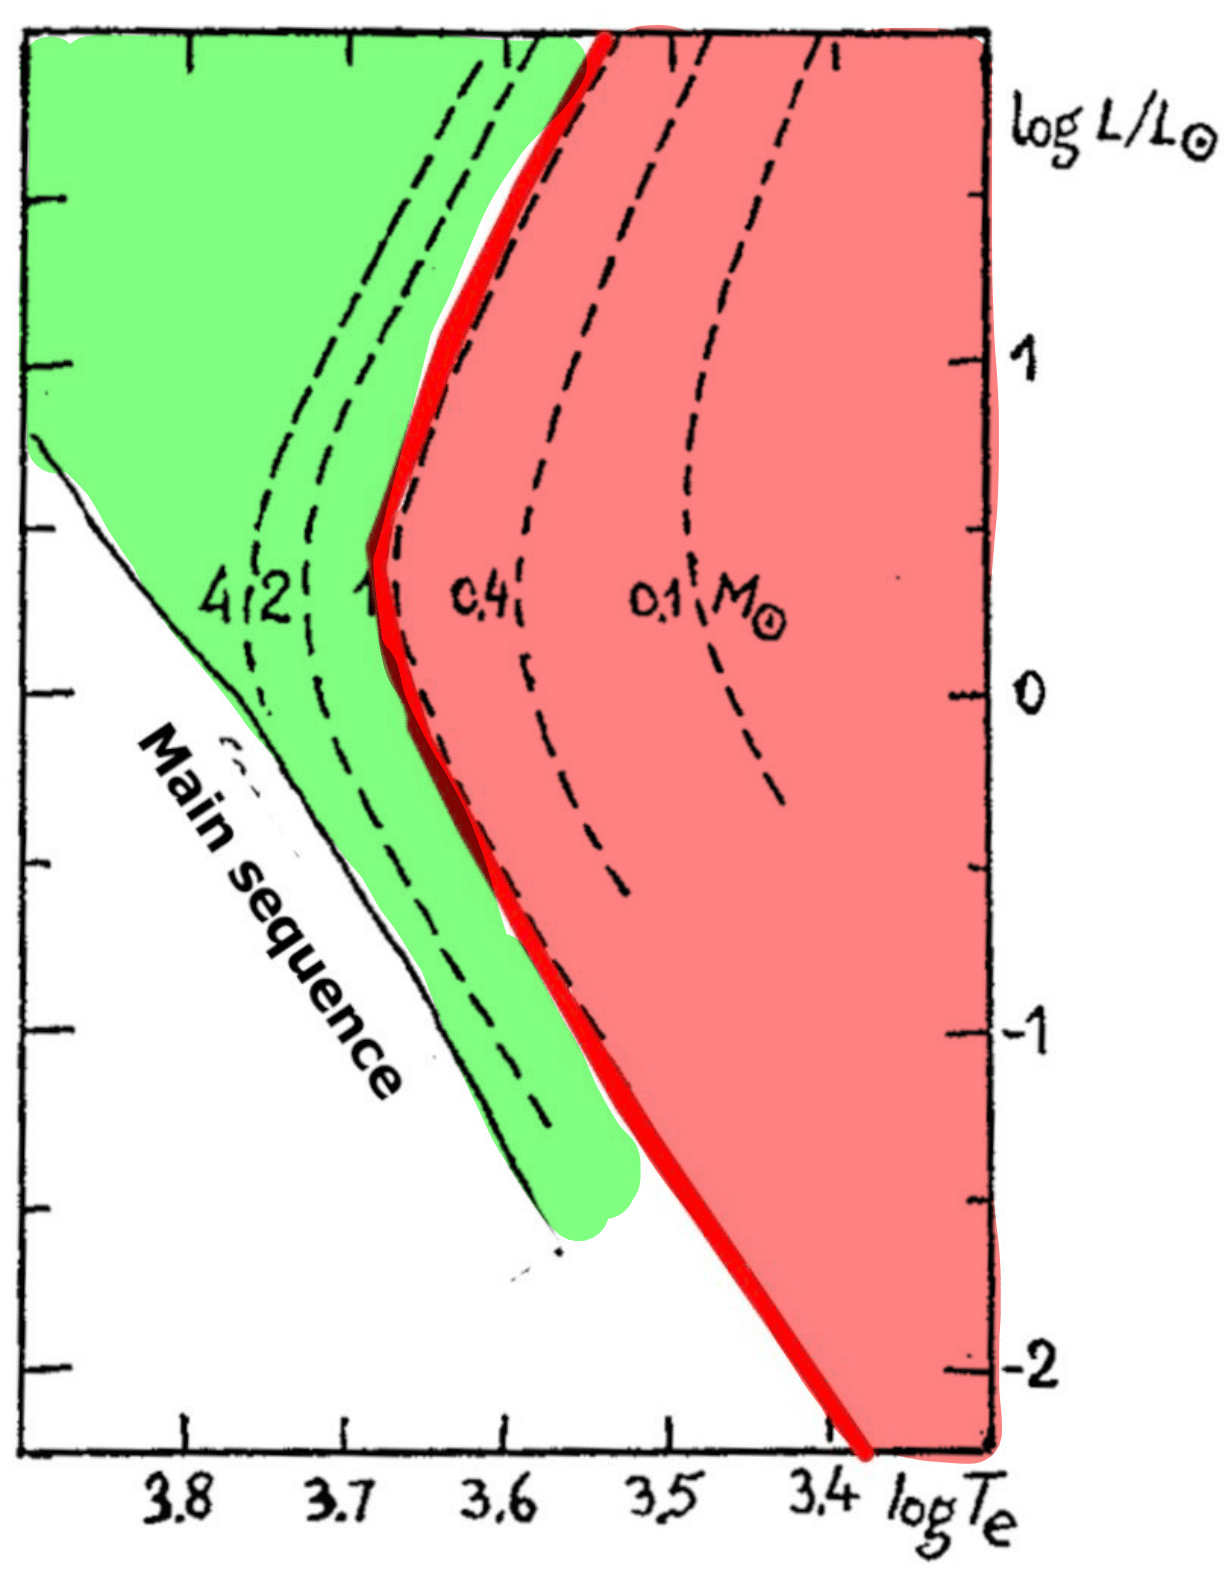
\includegraphics[width = 0.3 \textwidth]{immagini/hayashi-1.png}
    \caption{La figura mostra un diagramma H-R dove è stata evidenziata la traccia di Hayashi in rosso. A destra e a sinistra di questa sono state evidenziate due regioni, una in rosso ed una in verde. La prima mostra la zona in cui non è possibile generare stelle in equilibrio idrostatico, mentre la seconda mostra una regione di stabilità parzialmente convettiva.}\label{fig:hay}
\end{figure}

Particolarmente importante è la posizione di questa zona d'instabilità e della conseguente traccia di Hayashi. Infatti, queste si trovano nella parte fredda del diagramma H-R e, per quanto visto precedentemente, minore sarà la temperatura, maggiore sarà l'opacità della stella. Questo implica un gradiente radiativo maggiore di quello adiabatico ($\nabla_{\mbox{rad}} > \nabla_{\mbox{ad}}$) e quindi la presenza di convezione.

La fase di protostella dura fino a quando il nucleo raggiunge una temperatura $T \sim \SI{e7}{K}$, necessaria ad attivare le reazioni termonucleari. La durata di questa fase della vita della stella è compresa tra i $10^4$ e i $10^7$ anni, a seconda della massa iniziale della stella (maggiore è la massa iniziale, minore sarà la durata). Si tratta di una parte relativamente breve dell'evoluzione stellare.
\section{Main sequence}\label{sec:main-sequence}
\subsection{Zero-Age Main Sequence}
Dopo aver raggiunto le condizioni adatte per innescare le reazioni termonucleari, la stella comincia la parte più lunga della sua vita, detta Main Sequence (o MS), in cui brucerà idrogeno producendo elio ed energia. Sul piano H-R il punto iniziale della MS per una stella giace sulla Zero-Age Main Sequence (in breve ZAMS), una traccia che descrive la luminosità di stelle con la stessa composizione chimica, ma massa differente.

Non tutte le protostelle riescono ad accedere a questa parte dell'evoluzione stellare, infatti, esistono dei limiti al valore che la massa può avere. Data una protostella di massa superiore a $90 \si{\solarmass}$, la pressione di radiazione è così elevata che sovrasta quella gravitazionale disperdendo le parti più esterne. Per stelle con metallicità molto bassa questo limite può raggiungere anche le $300 - 500 \si{\solarmass}$ così come accadeva per le prime stelle. Nel caso in cui, invece, la massa è inferiore alle $0.08 \si{\solarmass}$ allora le temperature nel core non sono abbastanza alte da permettere l'attivazione delle reazioni termonucleari.

\begin{figure}
    \centering
    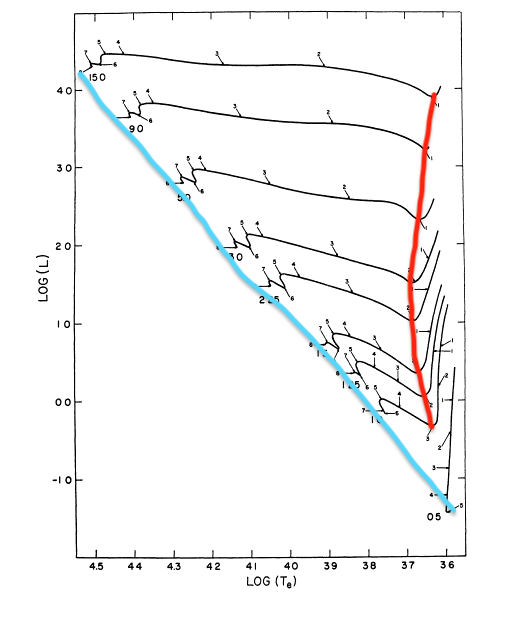
\includegraphics[width = 0.5\textwidth]{immagini/ZAMS.png}
    \caption{La figura mostra la Zero-Age Main Sequence in rosso e la traccia di Hayaschi in azzurro.}\label{fig:ZAMS}
\end{figure}

\subsection{Produzione e trasmissione di energia}\label{sec:prod-tras-energia}

La natura dei meccanismi di fusione influisce anche sull'andamento della luminosità sulla ZAMS, in particolare per stelle molto massive, si ha un andamento che va come $L \propto M^{3.6}$, per quelle relativamente più leggere si ha che $L \propto M^4$.  Stelle più piccole hanno infatti temperature del core relativamente più basse rispetto alle stelle più pesanti privilegiando le reazioni a catena PP, che avvengono a temperature di circa $T_e = \SI{1.4e7}{K}$, piuttosto che la CNO, che avvengono nei corpi più pesanti, con temperature del nucleo di circa $T_e = \SI{1.8e7}{K}$. Il punto di passaggio tra i due tipi di reazione è molto stretto e si trova a luminosità di circa $L = 1.2 \si{\solarmass}$.

Il metodo di bruciare il proprio combustibile ha anche delle conseguenze sulla struttura interna della stella, in particolare implica la presenza o meno di convezione negli strati della struttura stellare. Distinguiamo tre possibilità a seconda della posizione che una stella assume sulla ZAMS\: se la massa è inferiore a $0.3 \si{\solarmass}$ allora la struttura sarà completamente convettiva, se la massa è compresa tra le $1.2 \si{\solarmass}$ e le $0.3 \si{\solarmass}$ allora il core avrà una natura radiativa e gli strati più esterni convettivi, mentre per stelle più pesanti di $1.2 \si{\solarmass}$ la situazione è invertita con il core convettivo e gli strati esterni radiativi. Il motivo di queste differenze risiede nel fatto che, nonostante le temperature variano poco, i meccanismi per generare energia sono profondamente diversi. Come visto nella sezione-\ref{sec:catena-pp}

\[
    \epsilon_{\mbox{\footnotesize{pp}}} \propto \rho X^2 T^5
\]
\[
    \epsilon_{\mbox{\footnotesize{CNO}}} \propto \rho X X_{\mbox{\footnotesize{CNO}}} T^{15}
\]

Per cui si ha che, per masse superiori a $1.2 \si{\solarmass}$, $\epsilon_{\mbox{\footnotesize{pp}}} \ll \epsilon_{\mbox{\footnotesize{CNO}}}$ se la temperatura aumenta, lo farà anche la produzione di energia, assieme alla luminosità. Da quanto visto precedentemente l'aumento di luminosità implica un flusso più intenso. Diventa per cui necessario dissipare questa energia più velocemente, attivando i processi convettivi. Se infatti il flusso aumenta allora aumenta anche il gradiente radiativo e nel momento in cui $\nabla_{rad} > \nabla_{ad}$ si attiverà la convezione nel nucleo.

Per stelle con massa inferiore alle $0.3 \si{\solarmass}$, invece, la totale natura convettiva deriva dal fatto che, per luminosità così basse, la ZAMS coincide con la traccia di Hayashi.

Nel caso intermedio, infine, la natura radiativa del core è dovuta al fatto che le temperature non sono abbastanza elevate ad innescare le \textit{catene CNO}, per cui la produzione di energia non è intensa come per le loro controparti più massive. La cosa peculiare per queste stelle, però, è la presenza di convezione nella zona esterna della sua struttura, sicuramente non dovuta alle elevate temperature. La spiegazione arriva dall'alta opacità di questi strati, infatti per

\[
    \kappa \propto T^{-3.5}
\]

al diminuire della temperatura l'opacità aumenta e di conseguenza lo fa anche il gradiente radiativo, fino a che $\nabla_{rad} > \nabla_{ad}$ condizione per cui si attiva la convezione in quegli strati.

\subsection{Main Sequence}\label{sec:main-sequence-sub}

Dalla ZAMS l'evoluzione stellare entra nella vera e propria main sequence, nella quale fonderà l'idrogeno in elio, modificando molto lentamente la propria composizione chimica. In questa parte della propria vita la stella si trova in uno stato di estrema stabilità, dovuta al fatto che la fusione d'idrogeno è il processo termonucleare più efficiente che esista, motivo per cui questa fase è anche quella più lunga. Ciò nonostante la effettiva durata è variabile della massa iniziale, in particolare il tempo che questa impiega nella MS è inversamente proporzionale alla sua massa iniziale, secondo la relazione 
\[
    t_{MS} \cong 10^{10}M^{-3}\mbox{ \footnotesize{(yr)}}
\]
Nella tabella~\ref{tab:MS} è mostrata la durata in anni della main sequence insieme alla massa iniziale, normalizzata a quella solare.
\begin{table}
    \centering
    \caption{Nella tabella sono riportati i valori della durata della main sequence in funzione dei valori della massa stellare, per un campione di stelle.}\label{tab:MS}
    \begin{tabular}{c|ccccccc}
        \toprule
        M [$\si{\solarmass}$] & 15.0 & 9.00 & 5.00 & 3.00 & 2.25 & 1.50 & 1.00\\
        \midrule
        $t_{MS}$ [yr] & $1 \times 10^7$ & $ 2.2 \times 10^7$ & $7 \times 10^7$ & $2\times 10^8$ & $5\times 10^8$ & $1.7 \times 10^9$ & $9\times 10^9$\\
        \bottomrule
    \end{tabular}
\end{table}

Si osserva che data una stella di circa $0.8 \si{\solarmass}$, la durata della sua MS ha lo stesso ordine di grandezza dell'età dell'universo ($t_{MS} \sim 13.9\times 10^9 \mbox{ yr}$). Questo vuol dire che stelle con massa inferiore ad essa e nate poco tempo dopo l'origine dell'universo, saranno ancora nel pieno della propria main sequence.
\section{Post Main Sequence}\label{sec:post-main-sequence}
Quando la stella finisce l'idrogeno all'interno del core si passa alla fase finale dell'evoluzione stellare, chiamata \textit{post-MS}. 

\subsection{Sub e Red Giant Branch}\label{sec:SGB-RGB}
In una prima parte della post main sequence il nucleo si contrae e la temperatura aumenta, assieme alla pressione, bruciando gli strati di idrogeno esterni al nucleo in una fase chiamata \textit{Herztsprung Gap} per stelle pesanti o \textit{SGB} per stelle più leggere. Nel frattempo, mentre il core, ora pieno di elio, continua a contrarsi aumentando di massa e aumentando la propria temperatura, l'envelope si espande raffreddandosi rendendola appunto una \textit{Gigante Rossa}. Nella figura~\ref{fig:evo} i punti 3, 4 e 5 del diagramma H-R rappresentano queste transizioni, osservando che, benché la temperatura decresca repentinamente, la luminosità della stella rimane pressoché costante. Dall'equazione~\refeq{eq:stefan-boltzmann}, sappiamo infatti che:
\[
    L = 4\pi \sigma R^2 T^4
\]
Perciò la diminuzione di temperatura e il relativo aumento di volume si compensano perfettamente cosicché la luminosità del corpo ci appaia invariata, durante tutta questa fase della vita stellare.

Per stelle poco massive, al termine della SGB, la diminuzione di temperatura implica l'avvicinamento alla traccia di Hayashi, per questo motivo la struttura stellare risponde aumentando il proprio raggio e conseguentemente la sua luminosità (corrispondente al segmento $5-6$ nella figura~\ref{fig:evo}). Per stelle più pesanti, invece, la variazione di luminosità non è così netta. 
\subsection{Flash dell'Elio}\label{sec:flash-He e Horizontal Branch}

A questo punto nei corpi più leggeri, si arriva ad un punto limite, detto limite di degenerazione elettronica, superato questo il gas non può più essere considerato perfetto ed il nucleo entra in uno stato di degenerazione. L'aumento di temperatura non riesce a contrastare quello di densità, rendendo il gas sempre meno comprimibile e ritardando l'innesco dell'elio. Nei corpi più massivi la struttura è termoregolata, per cui l'aumento di temperatura è seguito dall'aumento di pressione e del volume della stella, in modo tale da bilanciare la pressione di radiazione. In queste strutture il collasso del core è notevolmente più facile, innescando le reazioni termonucleari per la fusione dell'elio non appena la temperatura raggiunge $T \sim \SI{e8}{K}$.

La differenza tra le due possibilità si osserva anche nel diagramma H-R della figura~\ref{fig:evo}, dove per le ultime l'attivazione della fusione ad elio (passaggio dal punto 5 al punto 6) è molto rapida e non comporta una variazione significativa della luminosità. Per le stelle più leggere, invece, l'accensione della fusione ad elio avviene in condizioni di semi-degenerazione e ritardata (di circa $\sim 10^6 \mbox{ yr}$) a causa dell'assenza di termoregolazione, motivo per cui l'aumento di temperatura non coincide con l'aumento di pressione. Si raggiunge, quindi, uno stato d'instabilità termonucleare fino a che $\rho_c$ non aumenta bruscamente, facendo implodere il core, rimuovendo la degenerazione e provocando un'esplosione, alla quale ci si riferisce con il termine \textit{Flash dell'Elio}. Questa comporta una rapida espansione del volume del nucleo e quindi della stella intera a causa di moti convettivi.
\begin{figure}
    \centering
    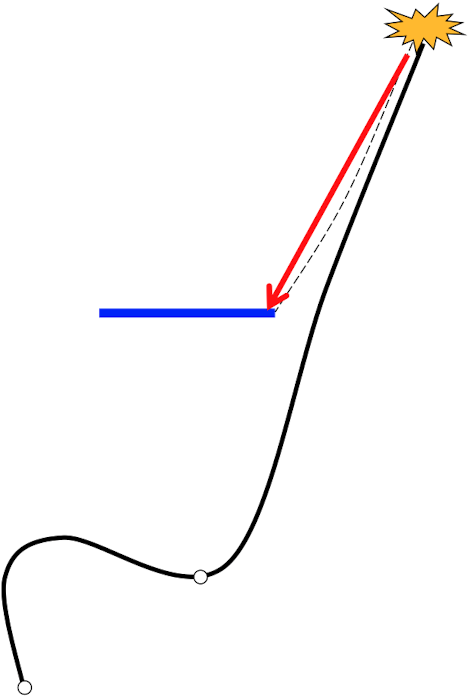
\includegraphics[width = 0.2\textwidth]{immagini/he_flash.png}
    \caption{La figura mostra la porzione del piano H-R in cui avviene il flash dell'elio assieme all'inizio dell' Horizontal branch.}\label{fig:flash-he}
\end{figure}

Dopo il flash dell'elio la produzione di energia diminuisce e così anche la luminosità della stella, fino a raggiungere la fase di \textit{Horizontal Branch} in cui questa rimane pressoché invariata. In questa parte della post-MS, raggiunta solo da stelle con massa inferiore alle $2.2 \si{\solarmass}$, non è presente degenerazione nel nucleo e si attiva la fusione di idrogeno negli strati più esterni della struttura, ancora pieni di idrogeno. Infatti, benché nel core l'idrogeno è stato consumato tutto durante la main sequence, negli strati più esterni, dove avveniva la trasmissione della radiazione, questo è ancora presente.

Nel piano H-R si osserva che l'esplosione dovuta all'accensione delle reazioni termonucleari ad elio avviene sempre quando la stella ha una massa intorno alle $0.5 \si{\solarmass}$ (nella figura~\ref{fig:evo} il punto 6 dell'evoluzione). Questo implica che la luminosità al momento del flesh dell'elio è uguale per tutte le stelle e che quindi tale fenomeno può essere utilizzato come indicatore di distanza dell'ammasso stellare, analizzando la magnitudine osservata e comparandola con quella assoluta.

Per stelle con una massa inferiore $M = 0.5\si{\solarmass}$ non è possibile attivare la reazione di fusione di elio nel core e per questo non sono in grado di attivare alcuna reazione termonucleare. Raggiungono quindi lo stato di \textit{Nana Bianca di elio (He Nana Bianca)}, una delle possibili morti stellari, in cui il nucleo rimane elettro degenere raffreddandosi lentamente, mentre gli strati più esterni rimangono liberi nella forma di nebulosa stellare.

Per quanto discusso nella sezione~\ref{sec:main-sequence}, una stella con massa inferiore a $M = 0.8 \si{\solarmass}$ passerà nella main sequence un periodo di tempo dell'ordine di grandezza dell'età del nostro universo. Inoltre, si è appena detto che le nane bianche si formano solo per stelle di massa inferiore a $M = 0.5 \si{\solarmass}$, questo vorrebbe dire che non è ancora possibile osservare questi tipi di corpi. Ciò nonostante questi corpi sono già presenti nei nostri cieli, com'è possibile? Quello che accade è che stelle nella fase SGB, con nuclei di elio, perdono i propri strati più esterni, per vari motivi (risucchio da parte di un'altra stella in sistemi binari, esplosione di una Supernova, ...).
\subsection{Asymptotic Giant Branch}\label{sec:asymptotic-giant-branch}

Si è arrivati al punto che le stelle con massa superiore a $M = 0.5 \si{\solarmass}$ sono in grado di riaccendere le reazioni termonucleari necessarie a fondere l'elio. Quando, però, finisce anche questo all'interno del core si arriva ad un bivio dettato ancora una volta dalla iniziale. 

Corpi con $M < 8\si{\solarmass}$ tornano in uno stato di nucleo degenere, ora composto da carbonio ed ossigeno, per cui non più in grado di attivare reazioni termonucleari, raggiungendo quello che viene chiamato il \textit{Ramo Asintottico delle Giganti (Asymptotic Giant Branch, AGB)}. La struttura di questa fase dell'evoluzione stellare è caratterizzata dall'attivazione della fusione negli strati più esterni, seguita poi dall'accensione della fusione dell'elio in quelli più interni (come mostrato in figura~\ref{fig:AGB}) in condizione di semi-degenerazione.
\begin{figure}
    \centering
    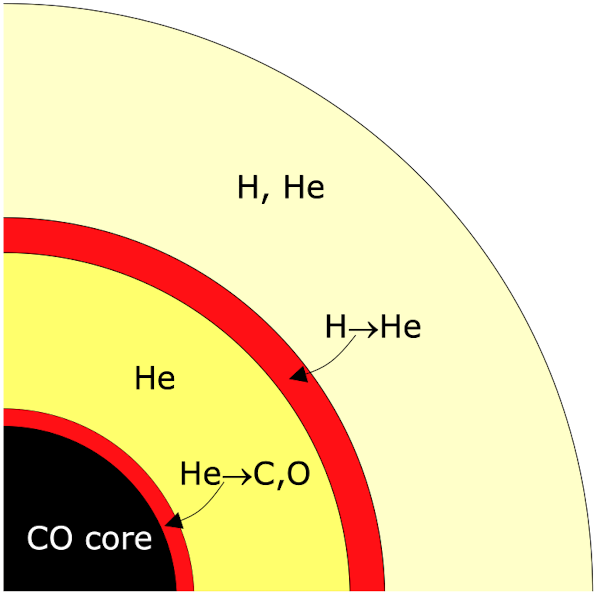
\includegraphics[width = 0.3 \textwidth]{immagini/AGB.png}
    \caption{La figura è una rappresentazione stilizzata della struttura stellare dopo la fine della fusione dell'Elio nel nucleo. Si osserva come negli strati dell'envelope si attivi la fusione di elementi progressivamente più leggeri allontanandosi dal centro della stella.}\label{fig:AGB}
\end{figure}
Quando anche l'elio si spegne, la stella si contrae e si attivano nuovamente le reazioni di fusione dell'idrogeno, osservando periodiche espansioni e contrazioni in un fenomeno chiamato \textit{Pulsazioni Termiche delle AGB (Thermal Pulse AGB)} dovute alla fusione periodica d'idrogeno ed elio. Nel piano H-R queste trasformazioni seguono la traccia di Hayashi parallelamente. Durante questi processi l'attrazione gravitazionale, per unità di superficie, sugli strati più esterni diminuisce a causa delle espansioni, comportando una perdita di materia rilasciandola nell'universo ad un rate di $\dot{M} \sim 10^{-4} \si{\solarmass} \mbox{ yr}^{-1}$. Si tratta di quasi una massa solare ogni $10000 \mbox{ yr}$, raggiungendo lo stato di \textit{Nebula planetaria} in cui non è più possibile attivare alcuna reazione termonucleare.

In questa ultima fase gli strati di elio ed idrogeno non sono abbastanza massivi da poter osservare alcuna attività termonucleare. La stella è definitivamente spenta. Il core si contrae aumentando la sua densità fino a raggiungere uno stato di degenerazione, mentre l'envelope si espande diventando un ammasso polveroso e di molecole fredde, rimanendo negli intorni di dove una volta era presente la stella. Quando la superficie di ciò che rimane raggiunge una temperatura di $T \sim \SI{e4}{K}$ parte dei gas e polveri presenti cominciano a ionizzarsi formando una nebulosa planetaria, che inizialmente non permette di osservare cosa resta del nucleo, a causa dell'elevata opacità. Queste strutture sono composte dagli elementi chimici generati dalle varie fusioni nucleari, in particolare elementi di tipo \textit{s}, carbonio, ossigeno, litio ed elementi pesanti dovuti al CNO.
\section{Morte Stellare}\label{sec:morte-stellare}
\subsection{Nane Bianche}\label{sec:nane-bianche}
Per stelle con massa $M < 8\si{\solarmass}$, in seguito al collasso gravitazionale del nucleo, dovuto all'assenza di reazioni termonucleari, la densità aumenta vertiginosamente raggiungendo $\rho \sim \SI{e6}{g.cm^{-3}}$. In queste condizioni si raggiunge l'equilibrio idrostatico tra pressione gravitazionale e pressione degli elettroni degeneri, dando luogo alla nascita di una \textit{Nana Bianca}.

Nel caso di nuclei a Carbonio e Ossigeno, è presente un sottilissimo strato non degenere di Elio ($M_{He} \sim 10^{-2} M_{WD}$) ed uno ancora più sottile di Idrogeno ($M_{H} \sim 10^{-4} M_{WD}$), sempre non degenere. 

\begin{table}
    \centering
    \caption{Nella tabella sono indicate le proprietà del corpo celeste noto come Sirius B, una nana bianca delle dimensioni simili a quelle terrestri, ma con massa comparabile con quella del sole, rendendolo un corpo estremamente denso.}\label{tab:sirius-b}
    \begin{tabular}{c|c}
        \toprule
        Proprietà & Valori\\
        \midrule
        M & $\sim 1.05 \si{\solarmass}$\\
        R & $\sim \SI{5.5 e8}{cm}$\\
        $\rho$ & $\sim \SI{e6}{g.cm^{-3}}$\\
        T & $\sim \SI{2.7}{K}$\\
        \bottomrule
    \end{tabular}
\end{table}

Nel bilanciamento tra la forza gravitazionale e la pressione elettronica degenere la relazione che emerge
\[
    M^{frac{1}{3}}R = 3\times 10^{19}
\]
mostra che maggiore è la massa iniziale di una stella, minore sarà la sua dimensione della nana bianca. Questa relazione è stata ottenuta tenendo conto degli effetti dovuti alla relatività generale, la quale permette inoltre di trovare un limite al valore che la massa di elettroni degeneri può sopportare, detto massa di Chandrasekhar, e vale
\[
    M_{Ch} = 1.44{(1+X)}^2 \si{\solarmass}
\]
dove $X$ è la concentrazione di idrogeno.
Questa relazione non vale solo per questi corpi celesti, ma per tutte le strutture cosmiche tenute in equilibrio dalla pressione di elettroni degeneri, includendo anche le Nane Bianche di Elio (He Nane Bianche).

Supponendo che la massa di una nana bianca rimanga costante nel corso della sua evoluzione, assieme con il raggio, si osserva che la luminosità diminuisce contemporaneamente alla temperatura. La figura~\ref{fig:WD} mostra come si comportano nel piano H-R, a seconda della massa iniziale. L'evoluzione di una nana bianca risulta quindi parallela alle curve a raggio costante per tutta la durata della loro sequenza di raffreddamento.
\begin{figure}
    \centering
    \subfloat[]{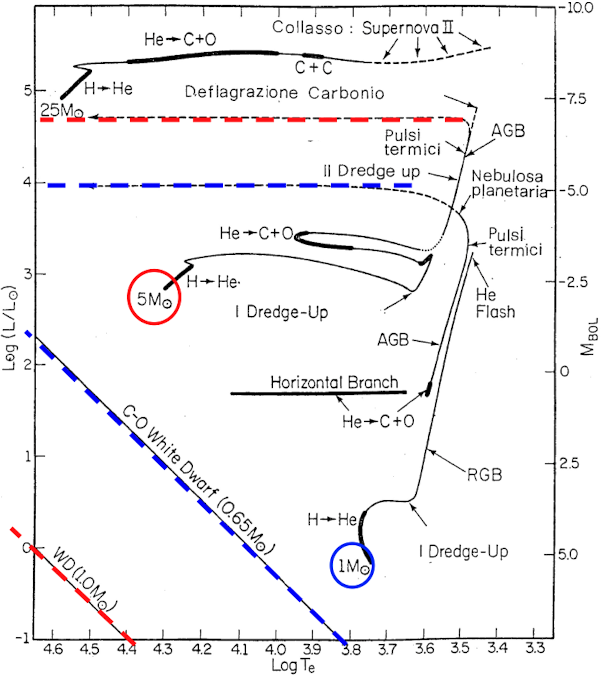
\includegraphics[width = 0.45\textwidth]{immagini/WD1.png}} \qquad
    \subfloat[]{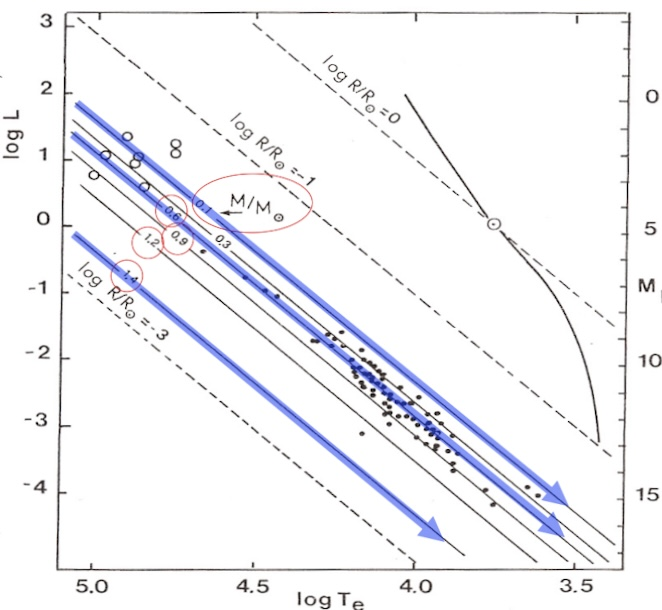
\includegraphics[width = 0.45\textwidth]{immagini/WD2.png}}
    \caption{L'immagine (a) mostra la differenza tra l'andamento dell'Horizontal branch per stelle leggere e delle nane bianche. Nella (b), invece, si apprezza come l'evoluzione di una nana bianca segua, nel piano H-R, l'andamento a raggio costante, ovvero una retta con coefficiente angolare negativo.}\label{fig:WD}
\end{figure}

La luminosità di questi corpi non sarà sicuramente dovuta alla presenza di reazioni termonucleari o all'energia gravitazionale proveniente dalla compressione del nucleo, ma all'energia interna, principalmente termica, del gas ionizzato. L'energia interna di una nana bianca è infatti data dalla relazione: 
\[
    U = \frac{M_{WD}}{A \cdot M_{H}} \frac{3}{2} k T_c
\]
e rappresenta una sorta di serbatoio energetico. In questo tipo di corpi il trasferimento di energia da una sezione all'altra avviene per conduzione.

I tempi di raffreddamento per una stella nana bianca seguono un andamento del tipo
\begin{equation}
    t_{cool} = 8.8\times 10^6 {\left(\frac{M}{\si{\solarmass}} \right)}^{\frac{5}{7}} {\left( \frac{L}{\si{\solarluminosity}} \right)}^{-\frac{5}{7}} \mbox{ yr}
\end{equation}
in cui fissate le luminosità, il tempo necessario a raffreddarsi diminuisce al diminuire della massa iniziale. Una nana bianca con luminosità costante a $L = 10^{-4.5} \si{\solarluminosity}$, ad esempio, a seconda che la massa sia $M = 1\si{\solarmass}$ o $M = 0.5 \si{\solarmass}$, avrà un tempo di raffreddamento di rispettivamente $\SI{12e9}{yr}$ o $\SI{7.6e9}{yr}$.

Il prototipo di stella Nana Bianca che è possibile osservare è Sirius B, lontana da noi quasi $8.6 \si{ly}$ e con le caratteristiche mostrate in tabella~\ref{tab:sirius-b}.

\subsection{Supernove}\label{sec:supernove}
Per quanto riguarda invece le stelle più massive, con $M > 8 \si{\solarmass}$, il nucleo non passa in uno stato degenere, ma rimane in condizioni di gas perfetto, innescando la fusione dell'Elio in Ossigeno o Carbonio, mentre nell'envelope viene bruciato l'Idrogeno rimanente in un tempo relativamente breve. Strutture stellari come queste non entrano mai in stato di degenerazione, ma rimangono termoregolate nel corso di tutta la loro evoluzione, fino ad arrivare alla fusione di elementi pesanti, con picco sul Ferro. Questa fase prende il nome di \textit{He Clump} e nella figura~\ref{fig:evo} tali processi sono rappresentati dai punti da 5 a 11, nella zona delle stelle massicce.

Per dare un'idea della durata delle varie fasi di fusione per diversi elementi, consideriamo una stella con massa iniziale pari a $M = 20\si{\solarmass}$ e indichiamo con $t_{X \rightarrow Y}$ la durata della fusione dell'elemento X in Y. I tempi caratteristici di ogni fase sono i seguenti:
\begin{description}
    \centering
    \item[$t_{H \rightarrow He}$] $\sim \SI{e7}{yr}$
    \item[$t_{He \rightarrow C}$] $\sim \SI{e6}{yr}$
    \item[$t_{C \rightarrow O}$] $\sim \SI{1000}{yr}$
    \item[$t_{O}$] $\sim \SI{200}{days}$
    \item[$t_{Si}$] $\sim \SI{7}{days}$
\end{description}

Man mano che si accendono fusioni di elementi differenti, negli strati più esterni della struttura stellare si attivano le reazioni termonucleari che fondono gli elementi più leggeri. Sia, per esempio, una stella che nel nucleo ha attive le reazioni per la fusione del Silicio in Ferro, allora negli strati dell'envelope si starà trasformando l'Ossigeno in Silicio, il Carbonio in Ossigeno, l'Elio in Carbonio e l'Idrogeno in Elio, come mostrato in figura~\ref{fig:onion}, in una struttura detta a cipolla.

\begin{figure}
    \centering
    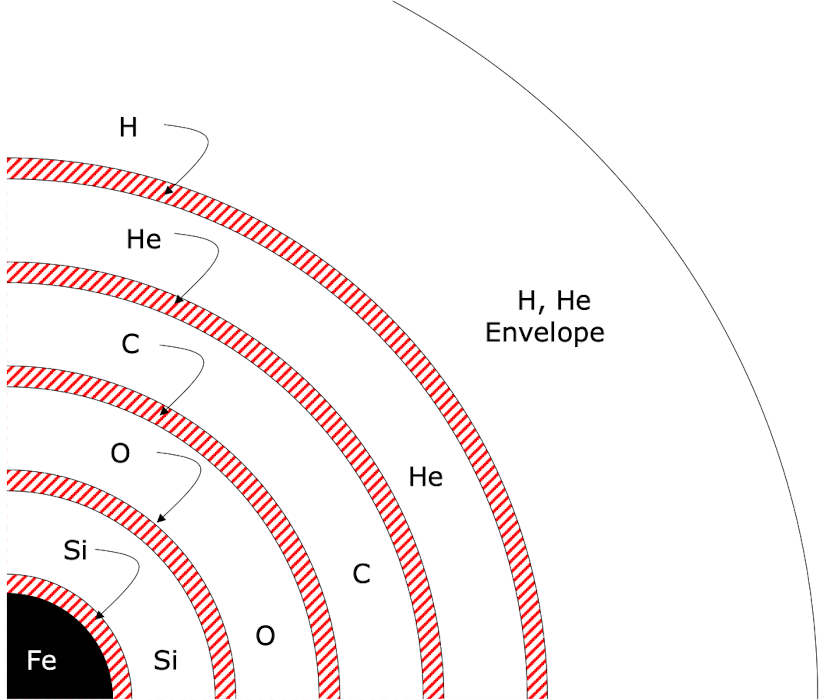
\includegraphics[width = 0.5\textwidth]{immagini/onion.png}
    \caption{La figura mostra uno schema della struttura della stella mentre nel nucleo si sta fondendo il Silicio in Ferro. Si osserva che allontanandosi dal centro, si trovano le reazioni di fusione di elementi progressivamente più leggeri.}\label{fig:onion}
\end{figure}

Una volta che il nucleo è arrivato alla produzione di Ferro, le reazioni si fermano, in quanto si tratta dell'elemento con energia di legame più elevata di tutta la tavola periodica e quindi dell'elemento più stabile in natura. Non essendoci, inoltre, più una struttura termoregolata, la stella comincia a contrarsi ed il nucleo diventa un gas di elettroni degeneri, all'interno del quale inizia ad avvenire la cattura elettronica. 

\reaction[re:ec1]{Fe^{56} + e^- -> Mn^{56} + \nu}
\reaction[re:ec2]{Mn^{56} + e^- -> Cr^{56} + \nu}

Data l'enorme temperatura all'interno del core ($T \sim 5-\SI{10e9}{K}$) si attiva quella che viene chiamata fotodisintegrazione del Ferro in Elio e dell'elio in protoni ed neutroni, come mostrato nella reazione~\ref{re:fotodis1} e  \ref{re:fotodis2}.

\reaction[re:fotodis1]{Fe^{56} + $\gamma$ -> 13He^4 + 4\eta}
\reaction[re:fotodis2]{He^4 + $\gamma$ -> 2p^+ + 2\eta}

Dato che l'energia dell'elettrone è superiore alla differenza di massa tra protone e neutrone, la cattura elettronica avviene anche da parte dei protoni, aumentando il numero di neutroni all'interno del core ed emettendo neutrini elettronici.

\reaction[re:pe]{p^+ + e^- -> \eta+ \nu_e}
Dal momento che la struttura era tenuta in equilibrio idrostatico grazie alla pressione degli elettroni degeneri, la loro diminuzione (reazione~\ref{re:pe}) , comporta il collasso del nucleo, quasi in cauta libera, in un tempo rapidissimo ($t \sim \SI{e-2}{s}$), assieme ad un enorme emissione di energia, proveniente dai neutrini. Data una stella con massa iniziale pari a $M = 20\si{\solarmass}$ la sua luminosità sarà $L \sim \SI{4.4e38}{erg.s^{-1}}$, mente l'energia dei neutrini sarà $E_\nu \sim \SI{3e45}{erg.s^{-1}}$, collassando, la densità del nucleo si avvicina a valori simili a $\rho = \SI{2.4e14}{g.cm^{-3}}$ (stesso ordine di grandezza della densità nei nuclei atomici), fino a che non si arresta bruscamente. A questo punto il core rimbalza (a velocità supersoniche), scontrandosi con gli strati esterni della stella, generando una violenta onda d'urto che si propaga velocemente, anche grazie alla presenza di neutrini. Questo perché il nucleo, collassando, diventa sempre più opaco a questi, forzandoli a interagire con la materia dell'envelope cedendo la loro energia e facendo raggiungere all'onda d'urto energie cinetiche dell'ordine di $\sim \SI{e51}{erg}$ ($v = 200-\SI{30000}{km.s^{-1}}$). Eventi di questo tipo vengono chiamati \textit{Supernove II}.

Dopo l'esplosione le temperature scendono da $\SI{2e5}{K}$ a $\SI{5000}{K}$, mentre l'idrogeno nell'envelope si combina in $\mbox{H}_2$, facendo tendere l'opacità a zero e rilasciando tutta l'energia che era stata intrappolata, osservando un picco nella curva di luminosità (figura~\ref{fig:supernova})
\begin{figure}
    \centering
    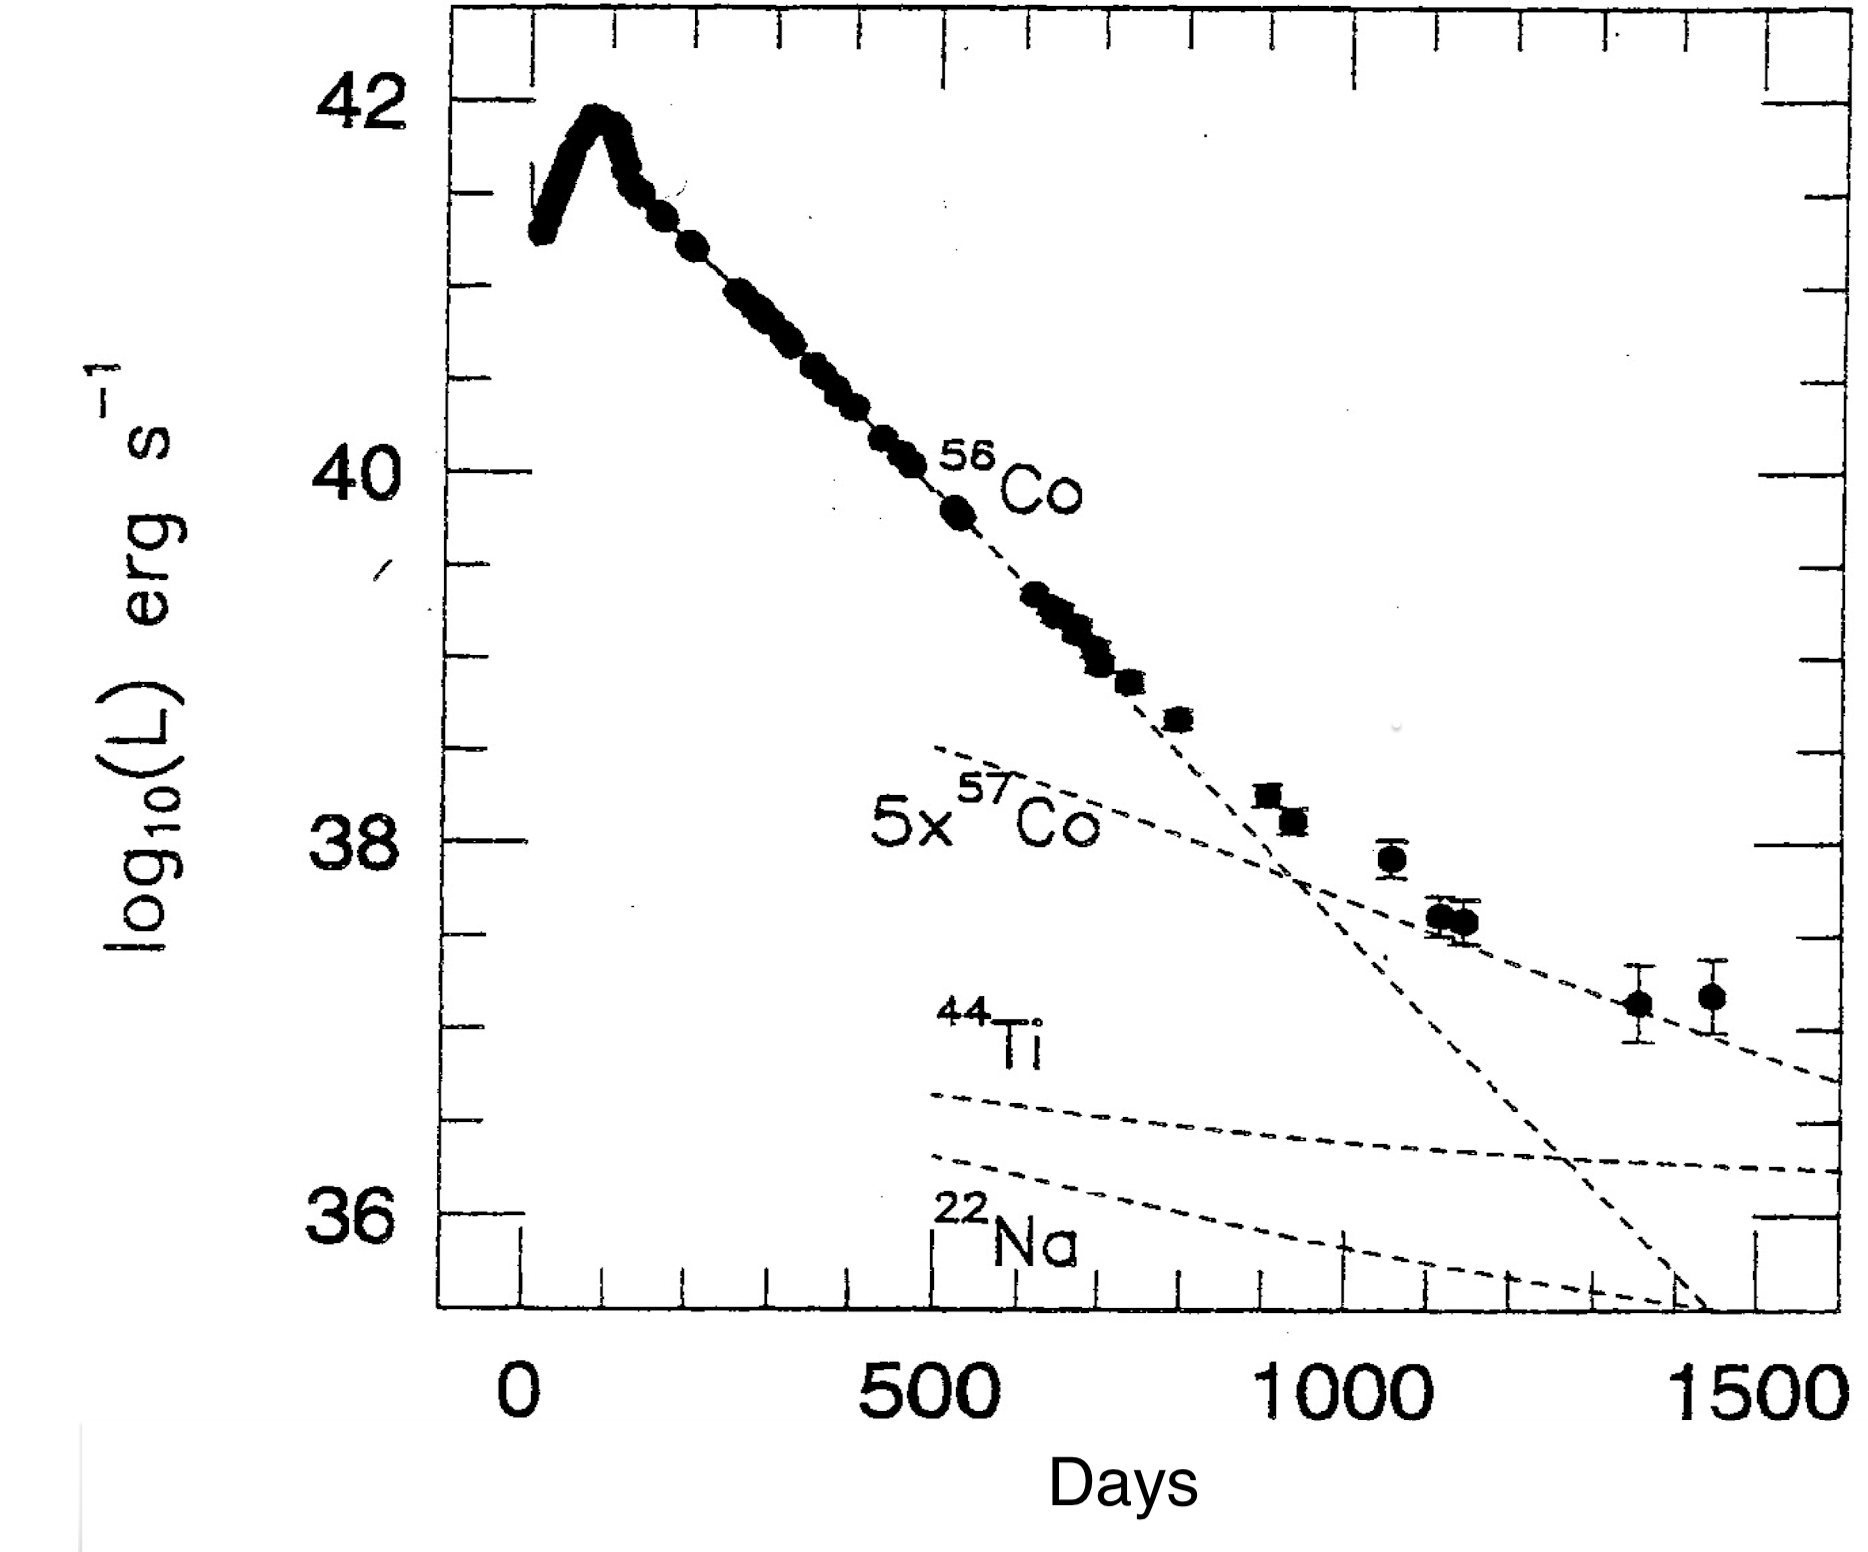
\includegraphics[width = 0.4\textwidth]{immagini/supernova.png}
    \caption{}\label{fig:supernova}
\end{figure}

Il Ferro che era presente nell'envelope è stato tutto tramutato in neutroni, mentre quello che era all'interno del nucleo, rimarrà nel nucleo, inaccessibile. La presenza di ferro nell'universo è dovuta principalmente alla fusione degli atomi di Silicio avvenuta durante l'esplosione della setalla, ma anche agli atomi di Nichel generati nella parte finale di questa, che decadono in Cobalto e successivamente in Ferro ($\tau_{1/2}^{\mbox{\scriptsize{Ni}}} = \SI{6.1}{days}$, $\tau_{1/2}^{\mbox{\scriptsize{Co}}} = \SI{77.1}{days}$).
\subsection{Classificazione delle Supernove} \label{sec:calss-supernove}

Una prima classificazione di questi eventi è quella spettrale, in particolare possiamo distinguere le seguenti supernove:
\begin{description}
    \item[supernova tipo I:] nelle quali NON sono presenti linee spettrali legate all'Idrogeno
    \begin{description}
        \item[tipo I.a:] con linee spettrali legate al Silicio;
        \item[tipo I.b:] con linee spettrali legate all'Elio, ma non al Silicio;
        \item[tipo I.c:] non presenta linee spettrali né del Silicio, né dell'Elio;
    \end{description}
    \item[supernova tipo II:] nelle quali sono presenti linee spettrali legate all'Idrogeno
\end{description}

Tale suddivisione non tiene conto, però, della fisica dell'esplosione. Risulta utile quindi introdurre una seconda classificazione che contiene la precedente, ma permette di descrivere il meccanismo di espansione:
\begin{description}
    \item[core-collapse]: di cui fanno parte le supernove di tipo II, I.b e I.c, soggette all'esplosione di una stella molto massiccia;
    \item[termonucleare]: di cui fanno parte le supernove di tipo I.a, soggette all'innesco esplosivo di una nana bianca CO che attrae massa da una stella vicina (sistema binario);
\end{description}

In particolare le supernove di tipo I.a possono innescare l'esplosione aggregando la massa da un'altra stella nana bianca (supernova I.a doppio-degenere) o assorbendo la massa di una stella ancora in MS vicina (supernova I.a singolo-degenere). In entrambi i casi non rimane nulla dei nuclei esplosi, ma l'energia rilasciata permette la creazione di elementi sul picco di Ferro. Una particolarità di questo tipo di supernove è che il picco di luminosità appare lo stesso indipendentemente dalla massa $M_{\mbox{\scriptsize{B, max}}} = - 19.6$ (\textit{Candela Standard}) e per questo motivo, vengono utilizzate come riferimento per studiare la distanza di oggetti nelle loro vicinanze (figura~\ref{fig:std-candle}), dall'analisi della loro luminosità.

\begin{figure}
    \centering
    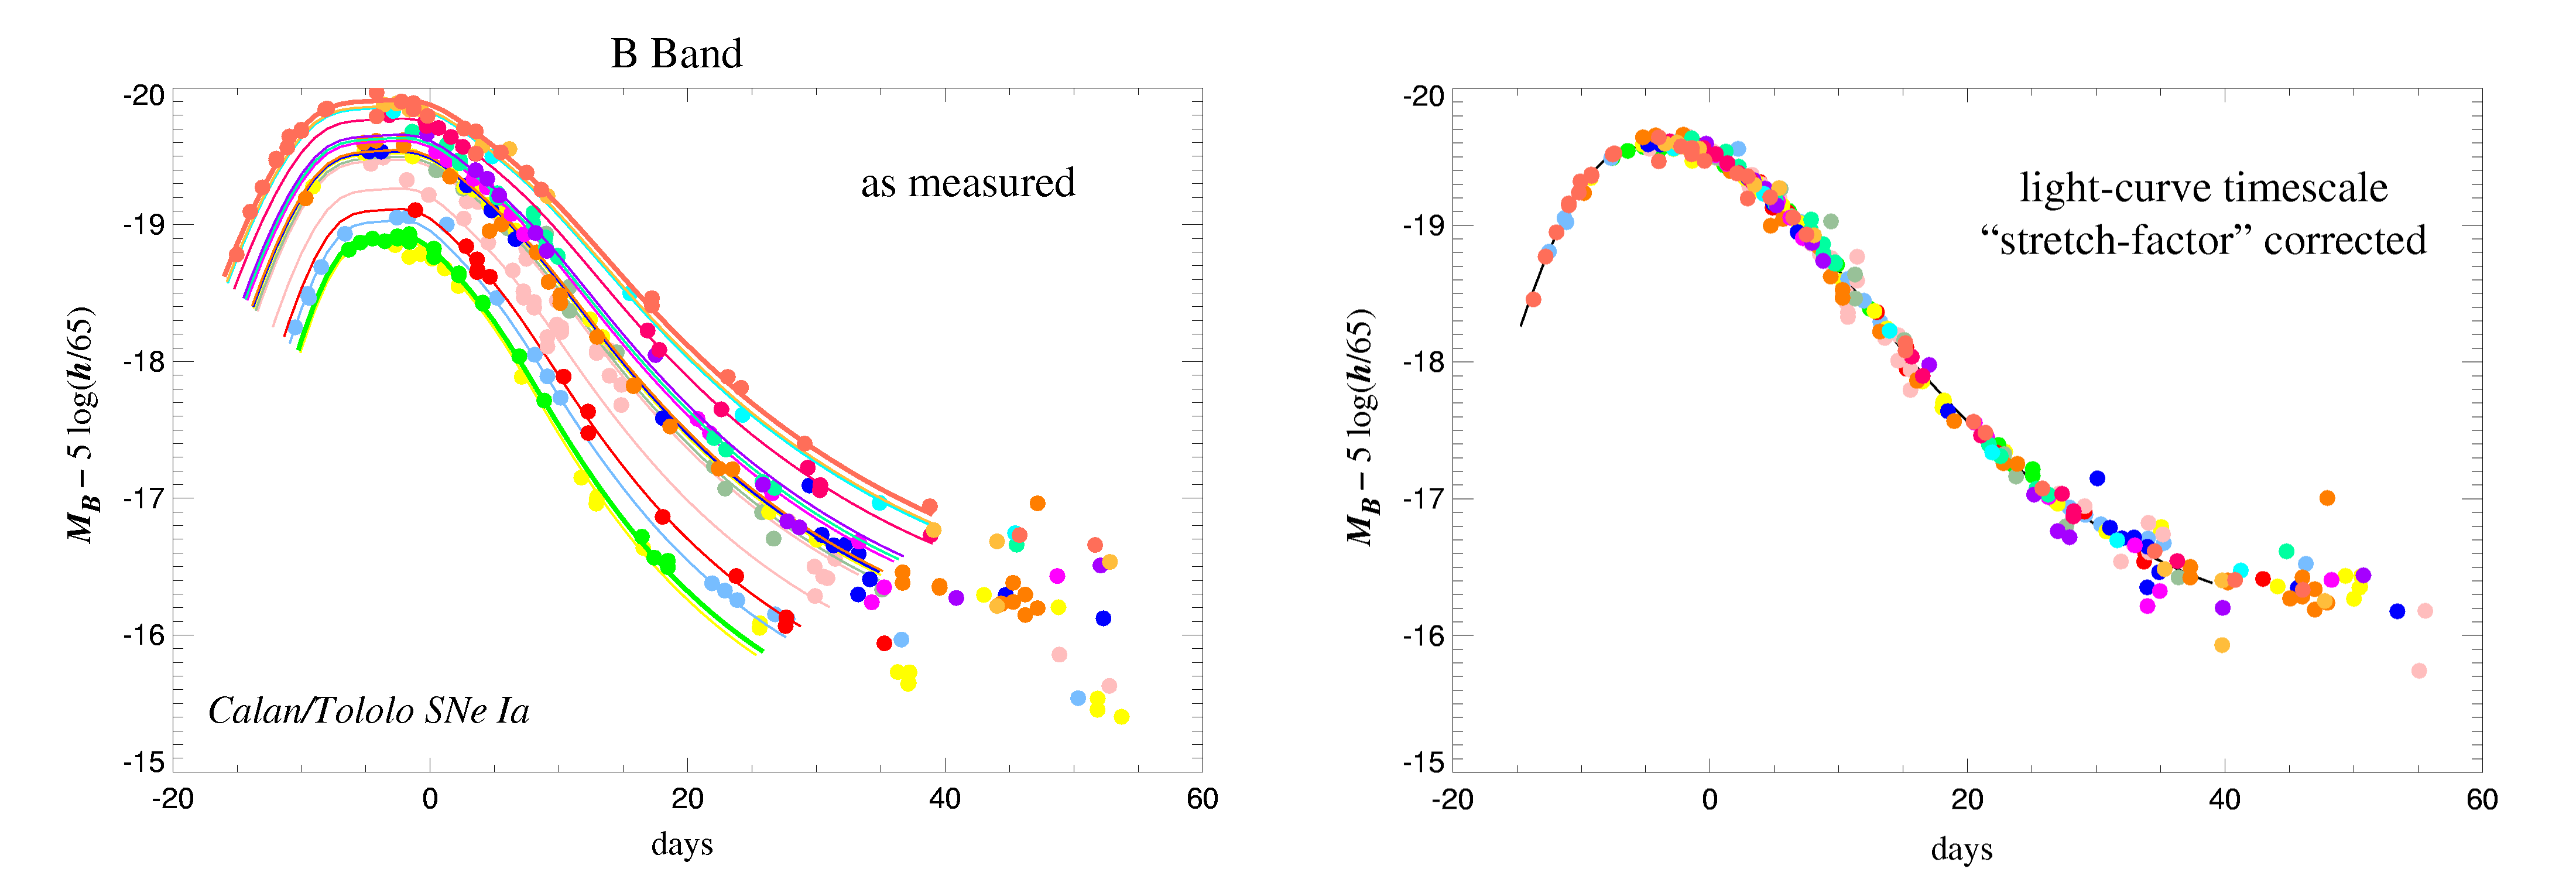
\includegraphics[width = \textwidth]{immagini/stretch_hammuy.png}
    \caption{La figura mostra la variazione di luminosità di alcune nane bianche in funzione del tempo, la (a) come sono state misurate, mentre la (b) corrette con il fattore di scala di allungamento.}\label{fig:std-candle}
\end{figure}

\subsection{Stella di Neutroni}\label{sec:stella-neutroni}
Dopo la supernova, se il nucleo non sparisce, come nel caso delle I.a, la natura dell'oggetto che rimane dipende dalla massa iniziale della stella. Si consideri inizialmente il caso $M < 25\si{\solarmass}$, nel quale si osserva la nascita di una \textit{Stella di Neutroni}. Si tratta di un corpo estremamente denso, tenuto in equilibrio idrostatico da un gas di neutroni degeneri, con le caratteristiche mostrate in tabella~\ref{tab:neutron-star}.
\begin{table}
    \centering
    \caption{La tabella riassume le principali caratteristiche di una stella di neutroni}\label{tab:neutron-star}
    \begin{tabular}{c|c}
        \toprule
        Caratteristica & Valore\\
        \midrule
        M&$\sim 1.2 - 1.5 \si{\solarmass}$ \\
        R&$\sim 10 - \SI{15}{km}$ \\
        $\rho$&$\sim 10^{14} - \SI{e15}{g.cm^{-3}}$ \\
        $T_{\mbox{\scriptsize{spin}}}$& $\sim 0.2 - \SI{2}{s}$ \\
        $|\vec{B}|$& $\sim 10^{13} - \SI{e14}{G}$ (gaus)\\
        \bottomrule
    \end{tabular}
\end{table}

Questi corpi vengono osservati nella banda radio a causa dell'emissione di elettroni a sincrotrone, cioè del movimento di cariche relativistiche all'interno di un campo magnetico. Inoltre, dato che l'emissione di elettroni segue la direzione del campo magnetico e questo ruota con un periodo $T_{\mbox{\scriptsize{spin}}}$, non per forza nella stessa direzione dell'asse di rotazione della stella, allora si osserva una radiazione pulsante. Corpi di questo tipo vengono detti \textit{Pulsar}. Se fosse presente una stella compagna che li alimenta, queste prenderebbero il nome di \textit{Pulsar Arricchiti}, con un periodo di rotazione che generalmente è $\sim \SI{1}{ms}$.

Così come accade per nane bianche con elettroni degeneri, anche per le stelle di neutroni esiste un limite alla massa che queste possono avere al fine di mantenere l'equilibrio idrostatico tra le forze. Tale valore è discusso ancora oggi, ma sembrerebbe aggirerebbe intorno alle $M_[NS]^{max} \sim 2.5 - 3 \si{\solarmass}$ e viene detto limite di massa di Oppenheimer-Volkov. Il superamento di questo limite comporta il collasso gravitazionale di una stella in un corpo ancora più particolare.
\subsection{Buchi Neri}\label{black-holes}

Data una stella con massa iniziale superiore a $M = 25\si{\solarmass}$, l'auto-gravità dell'oggetto rimanente dall'esplosione è così forte e concentrata da far collassare il nucleo in un oggetto la cui velocità di fuga
\begin{equation}\label{eq:fuga}
    v^2 = 2 \frac{GM}{R}
\end{equation}
è superiore alla velocità della luce. Un Corpo celeste di questo tipo viene detto \textit{Buco Nero} ed è ciò che rimane dall'esplosione di una supernova di tipo II. L'equazione~\refeq{eq:fuga} permette di trovare quello che viene detto raggio di Schwarzschild:
\begin{equation}\label{eq:schwarzschild}
    R_S = 2 \frac{GM}{c^2}
\end{equation}

A questa distanza dal centro si trova \textit{l'Orizzonte degli Eventi}, una linea immaginaria oltre la quale non è possibile scappare all'attrazione gravitazionale del buco nero. Potenzialmente ogni corpo potrebbe raggiungere questo stato, se compresso abbastanza da avere $R<R_S$.

L'osservazione di questi oggetti risulta quindi complessa, dal momento che assorbono qualunque tipo di radiazione che li colpisce. Risulta necessario, quindi, ottenere non una visione diretta del buco nero, ma indiretta, ovvero osservando gli effetti, gravitazionali, che questo genera sui corpi vicini. In generale questo è viene fatto osservando delle stelle che orbitano attorno ad un oggetto che appare puntiforme ed estremamente massivo.

Un altro metodo per vedere i buchi neri è osservare l'emissione dei gas che lo orbitano nella spettro dei raggi-X (termicamente), radiazione generata dell'attrito con le altre molecole mentre spiraleggia attorno all'orizzonte degli eventi.

Un ultimo metodo per osservarli è studiare le onde gravitazionali generate da due buchi neri in fase di merging.
\begin{figure}
    \centering
    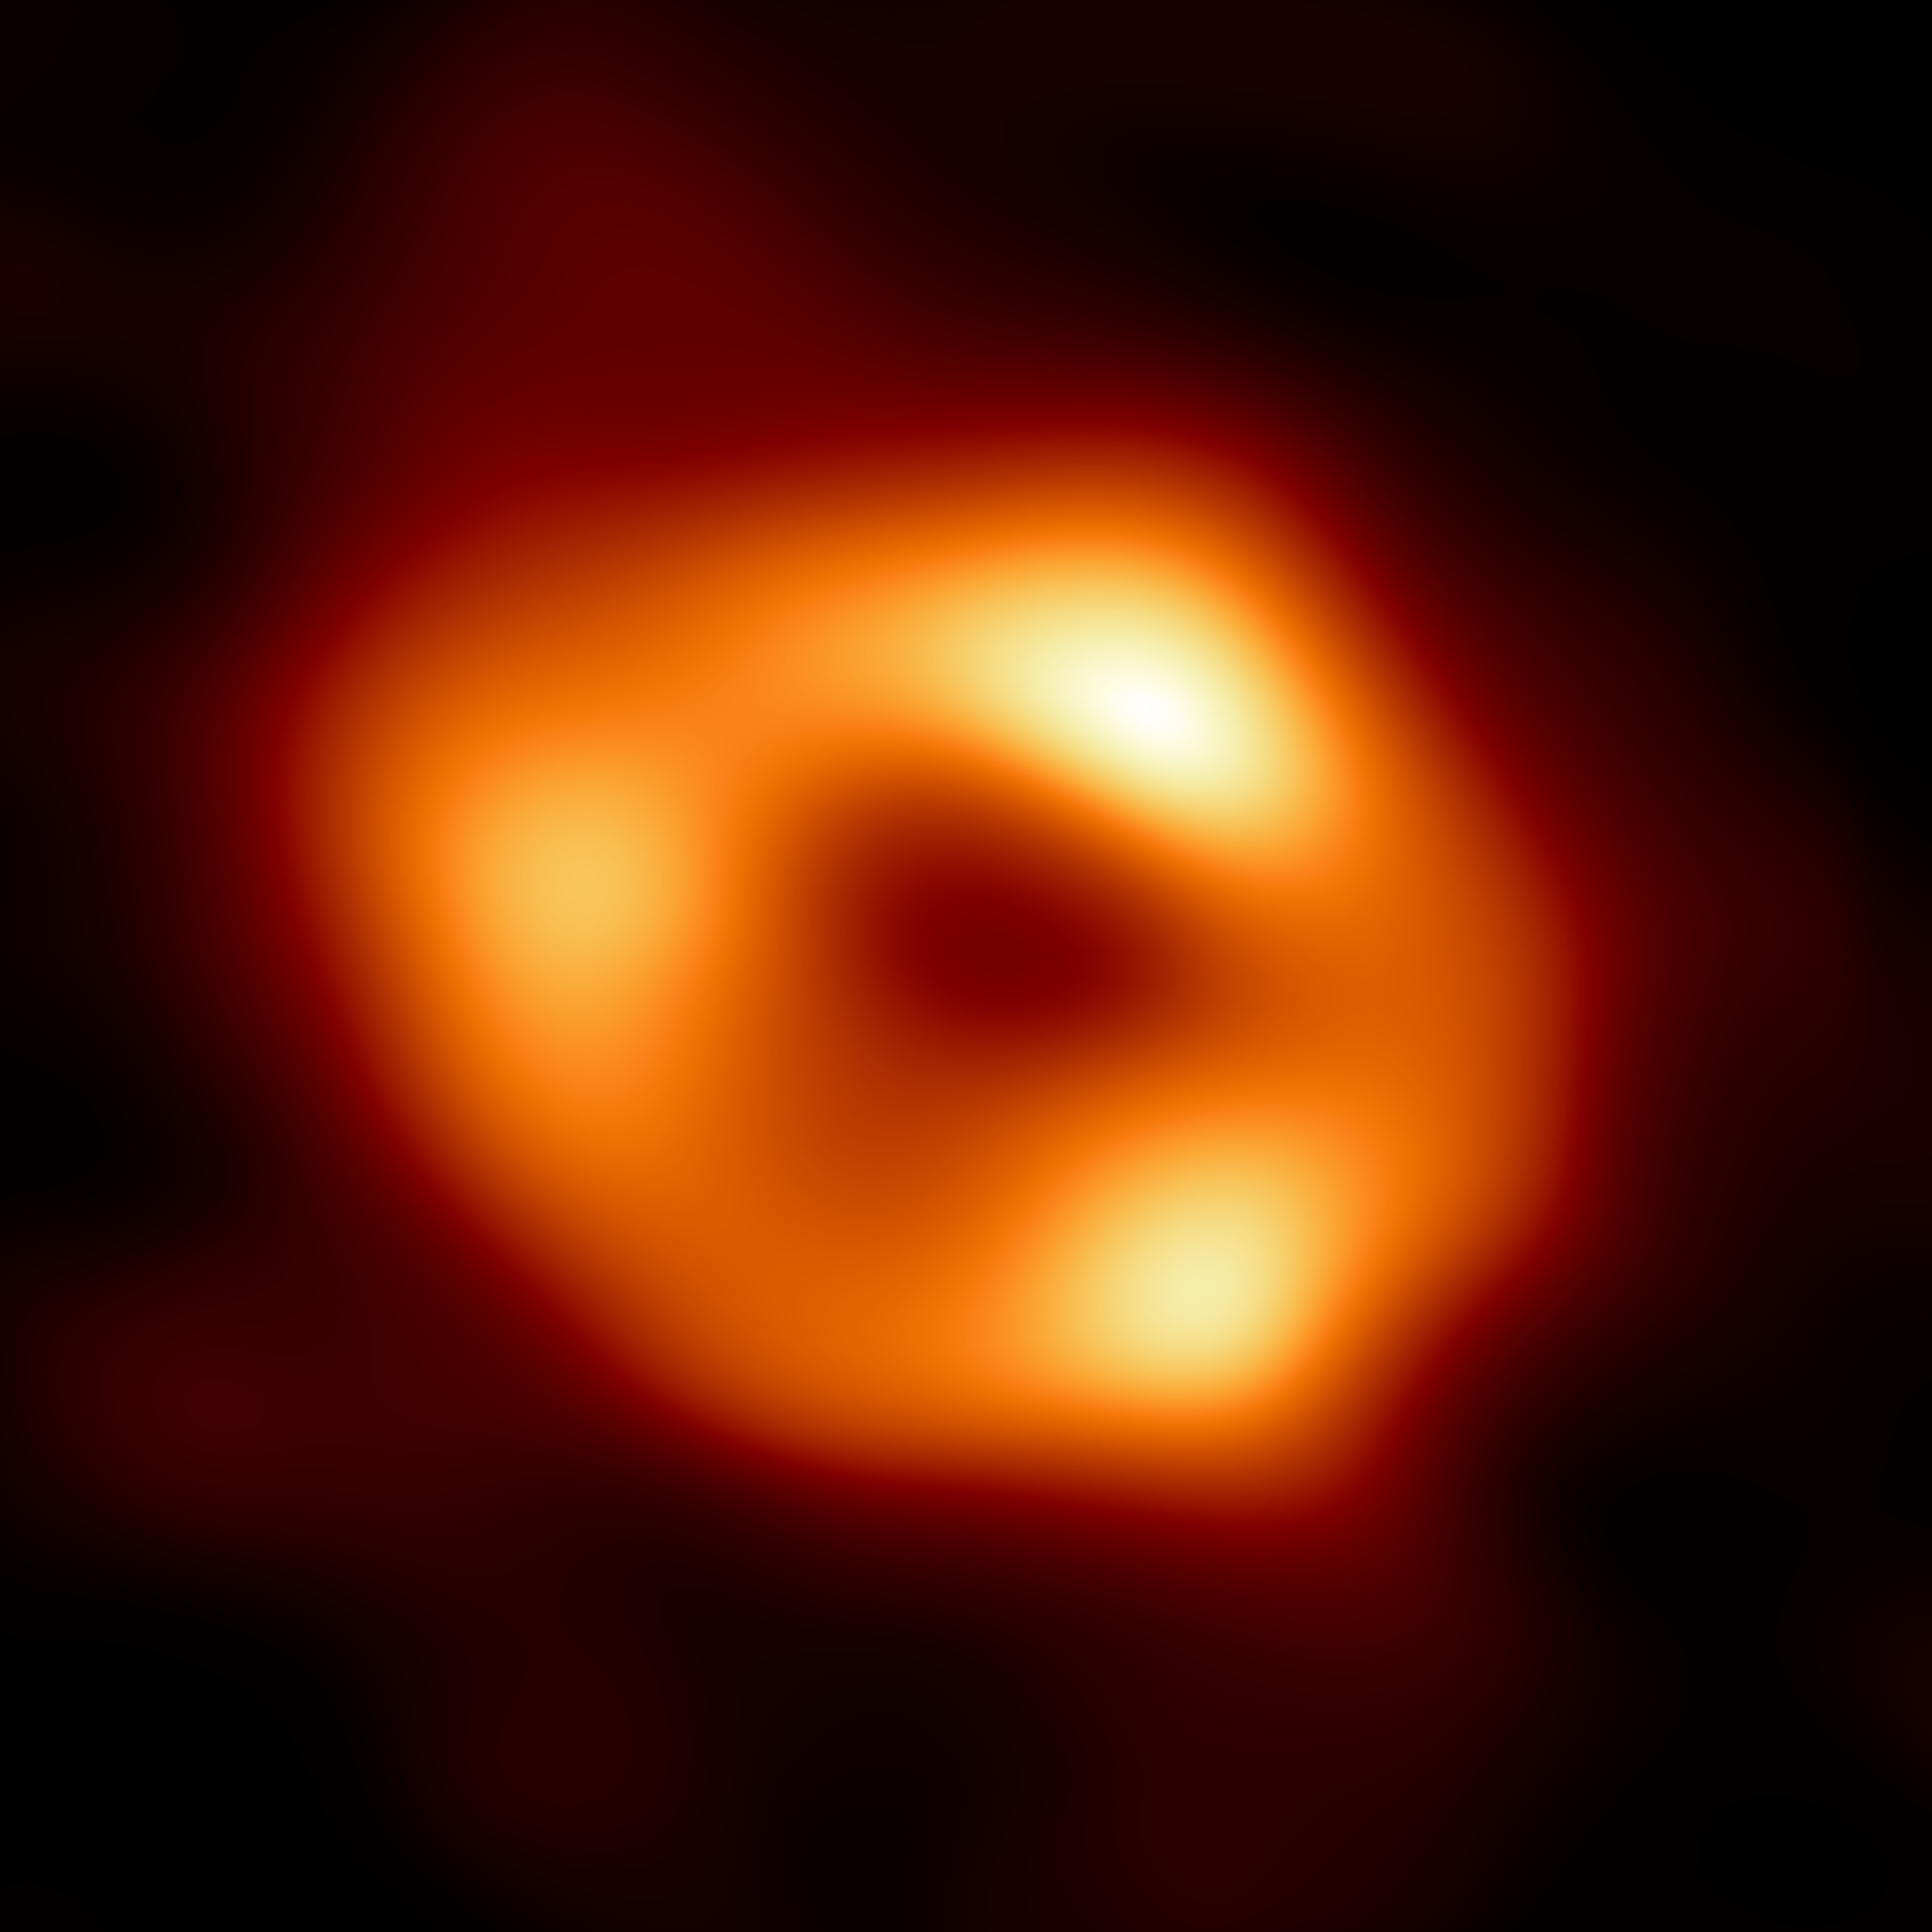
\includegraphics[width=0.4\textwidth]{immagini/blackhole.png}
    \caption{L'immagine ritrae il buco nero al centro della nostra galassia, attraverso lo studio della radiazione X emessa dai gas incandescenti in rotazione attorno ad esso.}\label{fig:buco-nero}
\end{figure}

Per quanto riguarda la massa di un buco nero stellare, invece, sappiamo dover aggirarsi intorno alle $50 - 100\si{\solarmass}$, ma conosciamo anche corpi di questo tipo decisamente più massicci. Questi vengono definiti con il termine \textit{Buchi Neri Supermassivi} e si tratta di oggetti di massa compresa tra le $10^6 \si{\solarmass}$ e le $10^9 \si{\solarmass}$, la cui origine è ancora oggi sconosciuta. Questo perché l'età dell'universo non è abbastanza grande da spiegare fenomeni di accrescimento così intensi, partendo da un buco nero stellare. Inoltre, sembrerebbe che esistessero già da poco dopo il Big Bang, benché non si sia ancora completamente sicuri di questo, dato l'elevato red-shift a cui sono soggetti. Il problema della loro esistenza sarebbe risolto se si venissero a scoprire dei buchi neri di taglia intermedia, con massa compresa tra le $10^2 \si{\solarmass}$ e le $10^5 \si{\solarmass}$.
\end{comment}


\chapterimage{cover/head10.jpg}
\chapter{Ammassi di Stelle}
\section{Ammassi Stellari}
All'interno del cosmo le stelle tendono ad aggregarsi in \emph{ammassi aperti} ed \emph{ammassi globulari}:

\begin{description}
\item[ammassi aperti:]costituite da un numero di stelle che si aggira tra i $10^2$ ed i $10^5$ elementi, tenuti insieme dalla mutua attrazione gravitazionale. Generalmente formate da stelle giovani e orbitano nel disco di galassie a spirale.
\item[ammassi globulari:]invece sono strutture decisamente più grandi, costituite infatti da un numero di stelle che si aggira intorno ai $10^5 - 10^6$. Questi sembrano trovarsi principalmente in orbita attorno agli aloni galattici, ma qualche volta anche attorno ai bulge (sec.~\ref{sec:classificazione-di-hubble}). 
\end{description}

Entrambe queste strutture sono caratterizzate dal fatto di essere costituite da stelle con la stessa età e composizione chimica, benché con masse differenti. Gli ammassi sono infatti degli ottimi luoghi per testare il modello di evoluzione stellare. Il modello che è stato studiato infatti, nel quale si è rappresentato l'andamento dell'evoluzione stellare all'interno dei diagrammi H-R, assume che il confronto tra stelle era possibile se fatto tra corpi di composizione chimica simile.

\begin{center}
    \begin{tikzpicture} [
            blu/.style={rectangle, draw=blue!60, fill=blue!5, very thick, minimum size=5mm},
            red/.style={rectangle, draw=red!60, fill=red!5, very thick, minimum size=5mm},
            green/.style={rectangle, draw=green!60, fill=green!5, very thick, minimum size=5mm},]
        \node[red](1){\footnotesize{Massa, X, Y , Z}};
        \node[blu](2)[right=of 1]{\footnotesize{Modello Stellare}};
        \node[green](3)[right=of 2]{\footnotesize{Evoluzione nel diagramma H-R}};

        \draw[->] (1.east) -- (2.west);
        \draw[->] (2.east) -- (3.west);
    \end{tikzpicture}
\end{center}

\subsection{Isocrone nel piano H-R}\label{sec:isocrone}

Andando a studiare le \emph{isocrone} del piano H-R si analizza il comportamento di stelle di massa differente, alla stessa età. Un esempio è la ZAMS o la figura~\ref{fig:isocrona}.

\begin{figure}
    \centering
    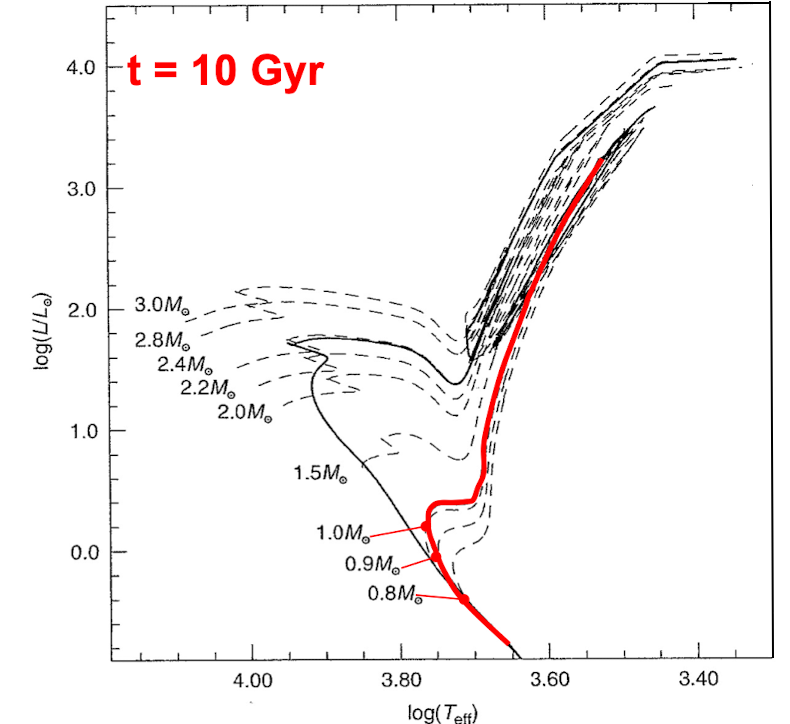
\includegraphics[width = 0.4\textwidth]{immagini/HR-isocrona.png}
    \caption{L'immagine mostra un'isocrona nel piano H-R, in rosso.}\label{fig:isocrona}
\end{figure}
\begin{figure}
    \centering
    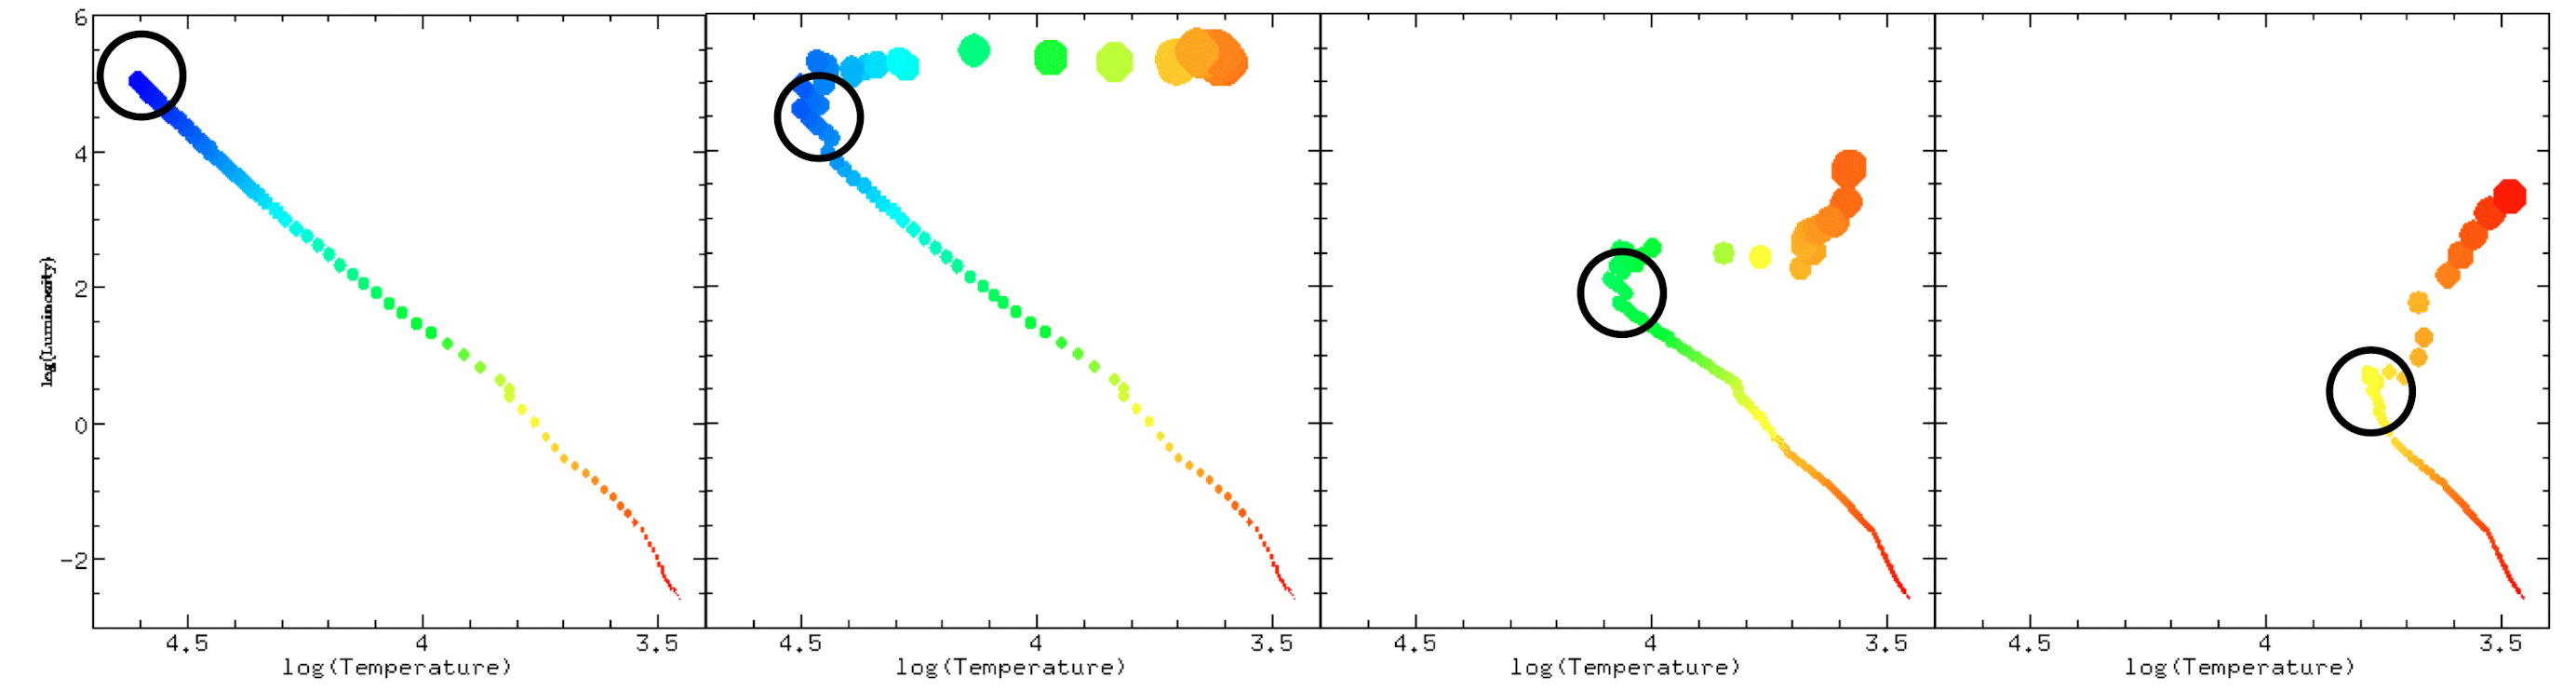
\includegraphics[width = 0.8\textwidth]{immagini/evoluzione-isocrona.png}
    \caption{L'immagine mostra come si evolve l'isocrona del diagramma H-R.}\label{fig:evoluzione-isocrona}
\end{figure}

Si noti, inoltre, come in figura~\ref{fig:evoluzione-isocrona} queste curve diminuiscano di lunghezza. Il motivo risiede nel fatto che all'avanzare del tempo le stelle più pesanti muoiono, infatti la durata della vita è inversamente proporzionale alla massa iniziale.

Si possono ora andare a studiare le sezioni principali di una isocrona. Per composizione chimica fissata ed età crescenti, si raggiungono in sequenza i seguenti punti:

\begin{enumerate}
    \item MS-TO (main sequence turning off point)\: al diminuire della massa, questo avviene a temperature e luminosità minori;
    \item Forma dell'MS-TO\: per stelle con una vita inferiore a $\SI{1}{Gyr}$ la forma è simile a quella di un uncino, mentre stelle con vita superiore da $\SI{1}{Gyr}$ assume una forma più arrotondata;
    \item Estensione della SGB\: l'estensione della SGB diminuisce al diminuire della massa iniziale della stella;
    \item Estensione della RGB\: al diminuire della massa aumenta il tempo che la stella impiega nel RGB;
    \item luminosità\: per stelle con una vita superiore a $\SI{1}{Gyr}$ viene raggiunta una densità costante.
\end{enumerate}
Si può avere un'idea della forma delle varie curve nella figura~\ref{fig:evoluzione-isocrona}, dove però non sono presenti le specificazioni dei vari punti.
\subsection{Prove Sperimentali}

Questo modello teorico rappresenta, però, quello che accade realmente in natura? Per rispondere a questa domanda bisogna però notare che luminosità e temperature non sono grandezze misurabili direttamente. Bisogna quindi costruire un diagramma equivalente a quello H-R per le osservazioni.

La grandezza che è possibile misurare da è la magnitudine apparente di un ammasso di stelle in due o più bande fotometriche (e.g. V e B), ottenendo quindi grandezze come magnitudine e colore. Costruiamo quindi un piano colore-magnitudine (CMD), sul quale posizionare ogni stella di un ammasso. Si ha infatti che il colore è una grandezza fortemente legata alla temperatura, mentre la magnitudine lo è con la luminosità.

Comparando l'andamento teorico e quello sperimentale nei due diagrammi (H-R e CMD) si osserva che effettivamente è presente un'ottima correlazione tra le due forme. Mostrando che effettivamente la risposta alla domanda iniziale è proprio sì, il modello teorico costruito predice in maniera eccellente quello che accade in natura (come mostrato in figura~\ref{fig:modello-osservazione-stellare}).
\begin{figure}
    \centering
    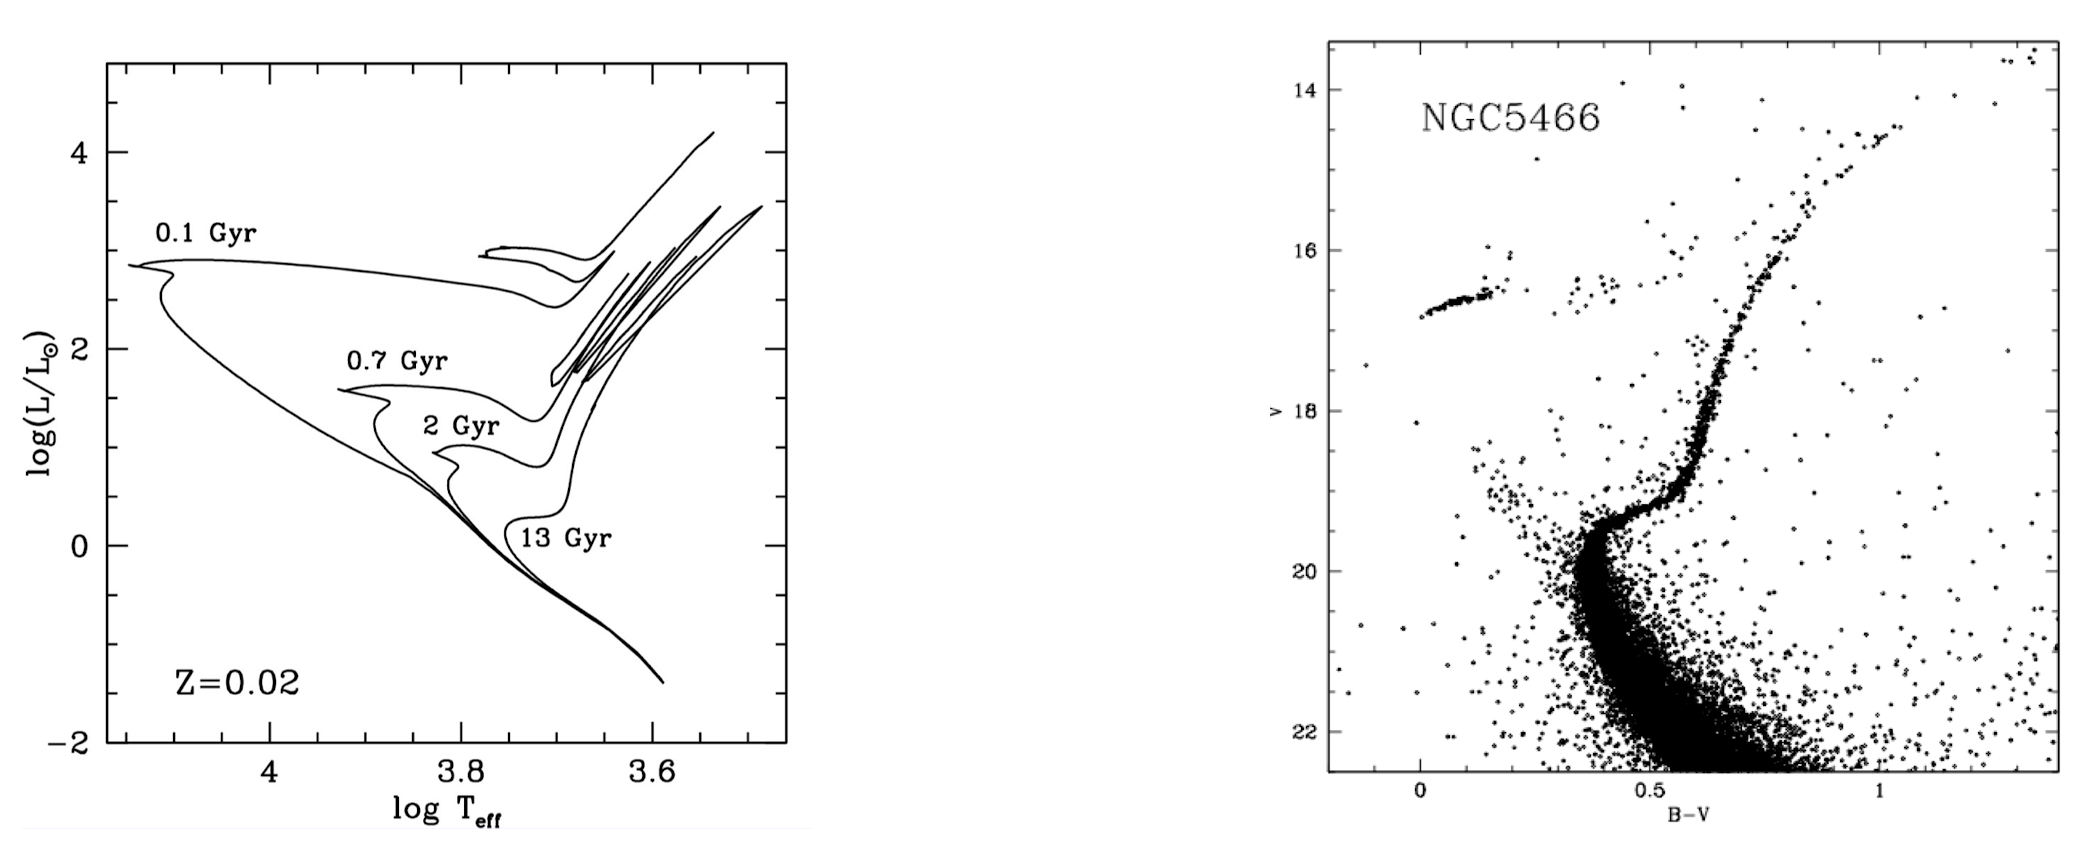
\includegraphics[width = 0.8\textwidth]{immagini/dati-sper-stelle.png}
    \caption{La figura mostra a sinistra l'andamento teorico del modello in un piano H-R, mentre a destra l'andamento dei dati sperimentali relativi a un ammasso stellare, in un piano CMD.}\label{fig:modello-osservazione-stellare}
\end{figure}

Lo studio degli ammassi stellari risulta, quindi, fondamentale per confermare ciò che viene dedotto nello sviluppo dei modelli stellari, ma non solo. Infatti vengono usati anche per l'analisi di alcune caratteristiche fisiche delle galassie, che non sono altro che un insieme di ammassi, ognuno con la propria età e con la propria composizione chimica.

In particolare per galassie abbastanza vicine è possibile utilizzare il CMD, in questo caso si dice che la galassia è \emph{risoluta}, mentre nel caso opposto \emph[non risoluta]. In quest'ultima non si può adoperare lo studio delle stelle per ottenere le proprietà della galassia.

\chapterimage{cover/head7.png}
\chapter{Galassie}
\section{Classificazione di Hubble}\label{sec:classificazione-di-hubble}
Le galassie sono sistemi celesti auto-gravitanti composti da circa $10^3$ - $10^7$ stelle, ma anche da polvere, gas e materia oscura. Sono l'unico posto dell'universo in cui possiamo trovare stelle, nello spazio interstellare NON sono presenti stelle isolate (a parte alcune nel mezzo inter-galattico degli ammassi di galassie e le prime stelle formatesi nell’universo, Pop III?).
Una prima classificazione delle galassie può essere fatta in base alla loro morfologia, individuando tre classi principali:
\begin{itemize}
	\item a spirale;
	\item ellittiche (o \textit{early-tipe});
	\item irregolari e peculiari.
\end{itemize}

Una classificazione ulteriore delle galassie è data dalla cosiddetta \emph{classificazione di Hubble}, che è rappresentata
dal diagramma a forcella in figura~\ref{fig:classificazione-di-hubble}:
\begin{itemize}
	\item Le galassie ellittiche sono classificate in base alla loro ellitticità, con un indice crescente da E0 a E7 (E0 corrisponde a una forma circolare, mentre E7 indica le galassie più ellittiche).
	\item Le galassie a spirale sono distinte in: spirali normali (S) e le spirali barrate (SB) e per entrambe ci sono sotto classificazioni: a, b, c. A seconda della lettera cambia il grado di avvolgimento dei bracci a spirale (Sa e SBa hanno bracci di spirale più avvolti intorno al nucleo rispetto a quelle Sc e SBc). Le galassie indicate con S0, anche dette lenticolari, sono galassie a disco che non mostrano evidenza di bracci nel disco.
	\item Come possiamo vedere le galassie irregolari e peculiari non sono incluse nella classificazione di Hubble.
\end{itemize}

\begin{figure}
	\centering
	\includegraphics[width=0.6\textwidth]{immagini/classificazione-di-hubble.png}
	\caption{Classificazione di Hubble}
	\label{fig:classificazione-di-hubble}
\end{figure}

La cosa più importante da tenere in considerazione quando si osserva il diagramma a forcella della classificazione di Hubble è che \emph{non si tratta di una sequenza evolutiva!} Non dobbiamo mai pensare che questo diagramma indichi che le galassie ellittiche evolvano verso galassie a spirale, è solo un modo per classificare il tipo di galassie esistenti.

\subsection{Galassie a spirale} Sono composte da dischi sottili con braccia a spirale e sono composte da stelle, gas e polvere con distribuzione non omogenea (le stelle sono organizzate lungo bracci a spirale). Al centro del disco c’è un rigonfiamento sferico chiamato bulge; attorno ad esso c’è un alone molto esteso quasi vuoto che presenta qualche ammasso globulare (alone costituito da molto meno materia rispetto al disco e al bulge). Nei bracci a spirale c’è formazione stellare in corso: ho stelle giovani, con età sotto 10 ml di anni e ricche di metalli (popolazione I), a causa della presenza di gas arricchiti dalle generazioni precedenti di stelle. Nel bulge e nell’alone non c’è formazione stellare in corso, quindi sono costituiti da stelle vecchie, con età sopra 12 mld di anni (popolazione II). Circa i 2/3 delle galassie a spirale sono spirali barrate, cioè oltre al bulge è presente una barra centrale ai cui estremi si diramano i bracci; anche la Via Lattea è una spirale barrata (SBc).

Una galassia a spirale è caratterizzata dalle seguenti caratteristiche generali:
\begin{itemize}
	\item \emph{MASSA:} $10^9 \si{\solarmass}$ fino a qualche $10^{11} \si{\solarmass}$ .
	\item \emph{DIMENSIONE (diametro):} da $\sim$ 5 kpc a varie decine di kpc.
	\item \emph{POPOLAZIONE STELLARE:} eterogenea (giovane e vecchia).
	\item \emph{COLORE:} soprattutto blu
	\item \emph{GAS, POLVERE:} soprattutto gas freddo; polvere nel disco, non nei bracci (dove c'è invece produzione stellare).
\end{itemize}

\subsection{Galassie ellittiche} Sono ellissoidi, costituiti essenzialmente da stelle di popolazione II, c’è pochissimo gas e pochissima polvere e ciò corrisponde al fatto che non c’è formazione stellare in corso (infatti le stelle si formano da gas freddo).

Una galassia ellittica è caratterizzata dalle seguenti caratteristiche generali:
\begin{itemize}
	\item \emph{MASSA:} da qualche $10^7 \si{\solarmass}$ (galassie ellittiche "nane") fino a $10^{12} - 10^{13} \si{\solarmass}$ (sono il tipo di galassia più massivo).
	\item \emph{DIMENSIONE (diametro):} da $\sim$ 1 kpc a varie decine di kpc.
	\item \emph{POPOLAZIONE STELLARE:} omogenea e vecchia ($5$ - $13$ Gyr).
	\item \emph{COLORE:} rosso
	\item \emph{GAS, POLVERE:} poco gas caldo (T $\sim$ $10^6/10^7$ K); no, poca polvere.
\end{itemize}

\begin{figure}
	\centering
	\includegraphics[width = \textwidth]{immagini/galassie-colore-magnitudine.png}
	\caption{In figura possiamo vedere una classificazione della magnitudine delle galassie in funzione del colore: notiamo come quelle che tendono più verso il rosso e sono più brillanti sono quelle di forma ellittiche. Le galassie a spirale risultano anch'esse abbastanza brillanti ma di colore blu (ci sono stelle più calde e più giovani).}
	\label{fig:galassie-colore-magnitudine}
\end{figure}

\subsection{Galassie irregolari e peculiari}
Sono galassie che non hanno una struttura riconoscibile, quindi non sono presenti bracci di spirale, disco o bulge riconoscibili; sono composte da un mix di gas e polvere, unito a stelle tendenzialmente di popolazione I. Molto spesso sono o galassie satelliti di altre galassie (quindi che ruotano attorno ad un'altra galassia) o sono in interazione con altre galassie e sono luoghi di intensa produzione stellare. Un esempio sono le due Nubi di Magellano (irregolari, perché hanno forma non ben definita), che sono galassie satellite della nostra galassia, ovvero risentono del potenziale della nostra galassia, e le Galassie Antenne (peculiari, perché hanno forma definita ma non canonica), che sono due galassie autointeragenti.

Una galassia irregolare o peculiare è caratterizzata dalle seguenti caratteristiche generali:

\begin{itemize}
	\item \emph{MASSA:} da qualche $10^7 \si{\solarmass}$ (galassie irregolari "nane") fino a $< 10^{10} \si{\solarmass}$.
	\item \emph{DIMENSIONE (diametro):} da $\sim$ 1 kpc a $\sim$ 10 kpc.
	\item \emph{POPOLAZIONE STELLARE:} soprattutto giovane.
	\item \emph{COLORE:} blu (per le "starburst" (quelle che formano stelle ad alto tasso) si ha colore rosso a causa della emissione della radiazione dalla polvere da cui si formano le stelle che riemette nel rosso come già visto in precedenza).
	\item \emph{GAS, POLVERE:} soprattutto gas freddo; polvere nel disco, non nei bracci (dove c'è invece produzione stellare).
\end{itemize}

\begin{figure}
	\centering
	\includegraphics[width = 0.6 \textwidth ]{immagini/galassie-colore-massa-stellare.png}
	\caption{In figura possiamo vedere un grafico che confronta colore e massa delle galassie: come possiamo notare le galassie ellittiche sono le più massive e verso il rosso, le galassie a spirale sono in parte verso il rosso e in parte verso il blu (con masse confrontabili con quelle ellittiche), mentre quelle irregolari sono quasi tutte blu e con masse molto minori.}
	\label{fig:galassie-colore-massastellare}
\end{figure}
\subsection{Effetti ambientali}
Il nostro universo non è riempito in modo omogeneo: sono presenti zone più dense (dette zone di cluster, dove avviene la formazione delle galassie), zone meno dense (dette ambienti di campo) e anche zone praticamente vuote, come si può vedere in figura~\ref{fig:non-omogeneo-universo}.

\begin{figure}
	\centering
	\includegraphics[width = 0.5\textwidth]{immagini/non-omogeneita-universo.png}
	\caption{In figura possiamo vedere rappresentate le tre tipologie di zone del nostro universo: cluster, ambienti di campo e spazio vuoto.}
	\label{fig:non-omogeneo-universo}
\end{figure}

Una domanda che sorge spontanea è: le diverse regioni di universo contengono stessi tipi morfologici di galassie oppure ci sono determinati tipi morfologici di galassie in diverse regioni di universo? Quello che è stato osservato è che negli ambienti di bassa densità (ossia gli ambienti di campo) c’è forte presenza di galassie spirali e irregolari (poche ellittiche e reticolari), mentre negli ambienti a più alta densità (ammassi di galassie) dominano le galassie reticolari e ellittiche (poche spirali), come è riassunto dal grafico in figura~\ref{fig:grafico-densità-morfologia}.

\begin{figure}[!htb]
	\centering
	\includegraphics[width = 0.5\textwidth]{immagini/enviromental-density.png}
	\caption{Nel grafico viene evidenziato come a basse densità siano presenti soprattutto galassie a spirale; all'aumentare della densità queste diminuiscono ed aumentano le galassie ellittiche e reticolari.}
	\label{fig:grafico-densità-morfologia}
\end{figure}

Perché abbiamo questa distribuzione? Le galassie nascono in questa maniera oppure vengono trasformate dall’ambiente? È l’ambiente che riesce a modificare il tipo morfologico delle galassie oppure nascono direttamente in quel tipo in quella regione particolare? In realtà è una domanda ancora aperta, infatti si contrappongono due visioni del fenomeno differenti:

\begin{itemize}
	\item Da una parte infatti si ha il modello cosmologico di Cold Dark Matter (il migliore attualmente), che prevede che le regioni di alta densità sono anche le regioni più vecchie (formate prima) e infatti si ha che le galassie ellittiche sono più vecchie delle altre. Questo quindi sembrerebbe aver senso col dato sperimentale. Ma perché allora sono proprio le ellittiche a formarsi prima? Anche a questa domanda non c’è ancora risposta.
	\item D’altra parte, sappiamo che ci sono molti processi fisici che hanno impatto nella morfologia delle galassie (ad es. ram pressure stripping, galaxy harassment…), in particolare in ambienti densi ci sono fenomeni che possono distruggere le spirali; infatti a causa dell'alta densità i bracci formati dalla galassia vengono strappati da quelle accanto, trasformandole tutte in ellittiche. Tuttavia, pensiamo che le ellittiche si formino da merge di galassie, e la probabilità di merge è più bassa per cluster più massivi (perchè le velocità relative sono troppo alte per permettere una collisione e successiva fusione).
\end{itemize}

Quindi in entrambi gli scenari ci sono problemi e la questione è ancora aperta.

\section{Spettro di emissione delle galassie}\label{sec:spettro-di-emissione-delle-galassie}
\subsection{Caratteristiche generali}
Per osservare le galassie viene ovviamente raccolta la radiazione proveniente da loro, ma essendo corpi celesti molto lontani otteniamo delle immagini spesso poco soddisfacenti, perché non è possibile distinguere le singole stelle che compongono la galassia (in quel caso si dice che stiamo osservando una popolazione stellare risolta). Per le galassie più lontane, per le quali la magnitudine non è risolvibile, la magnitudine è la cosiddetta \emph{magnitudine integrata} di tutte le stelle al suo interno: quello che osserviamo quindi è la cosiddetta luce integrata, che viene dalla somma di sorgenti non risolte per la maggior parte delle galassie (solo le stelle delle galassie del Gruppo Locale sono risolte, per le altre no). Allo stesso modo della luce, possiamo osservare che anche il colore di una galassia lontana è dato dall'integrale dei colori delle singole stelle e allo stesso modo possiamo applicare il medesimo ragionamento anche per uno spettro di risoluzione $\Delta\lambda$ finita. Quindi quando osserviamo la luce proveniente da una galassia in realtà stiamo osservando la luce che viene da diverse fonti: flusso o magnitudine integrata, colore integrato e spettro integrato con risoluzione $\Delta\lambda$ finita. Le normali tecniche di risoluzione stellare NON sono applicabili a galassie lontane.

Data una galassia, la luce che osserviamo provenire da essa sarà sicuramente emessa dalle stelle che la compongono ma non solo, abbiamo diverse origini:
\begin{itemize}
    \item Stelle: emissione fotosferica (UV - infrarosso intermedio), vento stellare (linee di emissione, IR da involucri di polvere), fenomeni di accelerazione (raggi X binari).
    \item Gas: freddo (idrogeno non ionizzato, nubi molecolari), tiepido (T $\sim$ $10^4$ K, linee di emissione, idrogeno ionizzato), più tiepido (T $\sim$ $2-3 10^4$ K, resti di supernovae, compressioni rapide del gas), caldo ( T $\sim$ $10^7$ K, raggi X, linee di emissione continua).
    \item Polvere: emissione termica (luce stellare riprocessata dalle interazioni, shock termico), caratteristiche di emissione/assorbimento (PAHs, silicati e grafiti), scattering (UV - luce infrarossa).
    \item Nucleo Galattico Attivo (AGN): non è presente in tutte le galassie, si tratta di un buco nero supermassiccio al centro di una galassia. Ci può essere emissione termica e non termica (spettro continuo e discreto). Nell'emissione termica lo spettro principale è quello dalle onde radio ai raggi gamma. La radiazione di un AGN può dominare l'intero spettro integrato.
\end{itemize}

In figura~\ref{fig:spettro+galassie} è riportato lo spettro di emissione (per lunghezza d'onda) delle galassie divise per morfologia: possiamo notare che determinate emissioni con una lunghezza d'onda precisa sono proprie della formazione stellare (osserviamo dei picchi in corrispondenza di quelle $\lambda$, come per OII e H$\alpha$) e infatti non appaiono in spettri di galassie in cui non si ha generazione stellare (passive, come quelle ellittiche o lenticolari). Lo spettro prende tutte le galassie; si potrebbe anche osservare la distribuzione spettrale di energia (SED) di una galassia in cui si verifica formazione stellare, che riporta solo un campionamento. Il confronto tra i due grafici (l'altro è sulle slide) è però in accordo con quanto riportato, si osservano quei picchi in entrambi i casi.

\begin{figure}
    \centering
    \includegraphics[width = 0.5 \textwidth]{immagini/spettro-galassie.png}
    \caption{Lo spettro della radiazione diviso per morfologia mostra come alcune lunghezze d'onda siano specifiche per galassie in cui si verifica formazione stellare}
    \label{fig:spettro+galassie}
\end{figure}

\subsection{Gas freddo, gas tiepido e polvere nelle galassie a spirale}
Come abbiamo detto una parte della radiazione proveniente dalle galassie proviene da gas freddo, in particolare da idrogeno neutro (H I); questo all'interno di una galassia è caratterizzato da una densità superficiale $ \sim 1 -\SI{10}{\solarmass.pc^{-2}}$, con un disco di dimensioni circa 5 volte maggiori dei dischi stellari (arriva fino a $\sim \SI{100}{Kpc}$). L'idrogeno neutro si osserva in banda radio, dal momento che l'emissione è di radiazione a lunghezza d’onda pari a $21$ cm. Perché avviene l'emissione? Si tratta di una transizione dovuta alla struttura iperfine dell’atomo di idrogeno. Il livello fondamentale dell’atomo di idrogeno è diviso in due sottolivelli: nel livello di più bassa energia il protone e l’elettrone hanno spin opposto, mentre il livello in cui gli spin sono uguali ha energia lievemente superiore (differenza di $6*10^{-6}\si{eV}$, corrispondente alla lunghezza d’onda di $21$ cm). Questa transizione è impossibile sulla Terra, avendo probabilità di emissione molto bassa, che corrisponde ad un'emivita lunghissima ($\tau \sim 10^7$ anni). Tuttavia, osserviamo tale transizione nell’universo a causa dell’elevata abbondanza di idrogeno, infatti la linea di emissione a $21$ cm è ben visibile sia per la Via Lattea, sia per altre galassie più esterne. La distribuzione di idrogeno neutro, inoltre, non è uniforme nel disco galattico: si ha infatti una zona di maggior densità (uguale per idrogeno ionizzato) lungo i bracci della spirale della galassia. 

L'idrogeno può comparire anche a temperature più alte e in quel caso si tratta di idrogeno ionizzato (H II): ci sono alcune regioni che si osservano in luce ultravioletta perché la radiazione viene emessa da stelle OB (stelle più calde – più giovani, hanno un'emissione così energetica che ionizza gas circostante, emettendo in banda UV). Stelle così calde si trovano in una zona di formazione stellare; osservare gas ionizzato è quindi indice della presenza di formazione stellare. Dal momento che questo fenomeno si osserva principalmente lungo i bracci delle galassie, se ne deduce che i bracci delle galassie a spirale sono luogo di formazione stellare. 

Per quanto riguarda invece il gas freddo e la polvere, questi sono osservabili in luce infrarossa, perché  per assorbimento (reddening) della luce, questa viene riemessa in banda infrarossa. 

\section{Struttura delle galassie a spirale}\label{sec:struttura-delle-galassie-a-spirale}
Analizziamo ora la struttura delle galassie a spirale: i dischi di spirale sono sempre in rotazione attorno al centro galattico. In quasi tutti i casi i bracci ruotano con bracci “trailing”, solo in pochissime galassie si hanno “leading arms” (fare riferimento alla figura~\ref{fig:trailing-leading-arms}): la forma a spirale quindi data dal materiale che viene trascinato dai bracci ma che si muove con velocità diverse. Infatti NON si ha rotazione rigida: la velocità angolare NON è la stessa in tutti i punti del disco. Si ha invece rotazione differenziale, quindi le stelle più vicine al centro ruotano con velocità più elevate; in genere la velocità tangenziale è la stessa indipendentemente dalla distanza dal centro, quindi le regioni più esterne hanno velocità angolare $\omega = V/r$ minore rispetto a quelle più vicine al centro. Questo significa che le stelle delle regioni più lontane dal centro impiegheranno decisamente più tempo per compiere un'orbita rispetto a quelle più vicine al centro.

\begin{figure}
    \centering
    \includegraphics[width=0.3\textwidth]{immagini/trailing-leading-arms.png}
    \caption{Differenza tra "trailing arms" e "leading arms": nel primo caso i bracci sono trascinati dalla rotazione, mentre nel secondo guidano e anticipano la rotazione.}
    \label{fig:trailing-leading-arms}
    \end{figure}

In seguito a questa osservazione nasce il cosiddetto "dilemma del winding", mostrato in figura~\ref{fig:winding-dilemma}: se i bracci fossero fatti da materia, allora dovrebbero avvolgersi attorno al centro galattico in tempi scala più corti dell’età della galassia stessa (dopo poche decine di rotazioni). Questo però comporterebbe la perdita dei bracci, che risulterebbero tutti avvolti su se stessi, ma non è quello che noi osserviamo; infatti siamo in grado di osservare bracci a spirale anche per galassie molto antiche. La risposta quindi è che questo “arrotolamento” non c’è anche se è presente rotazione differenziale. Ma perché non c'è?

\begin{figure}
    \centering
    \includegraphics[width =0.6\textwidth]{immagini/winding-dilemma.png}
    \caption{Dilemma del winding: se i bracci delle galassie fossero di materia dovrebbero pian piano arrotolarsi sul centro della galassia stessa.}
    \label{fig:winding-dilemma}
\end{figure}

La soluzione a questo quesito è basata sulla teoria di onda di densità di Lin: il fatto è che i bracci di spirale non sono materiali (quindi non sono composti da un insieme di gas e stelle che si muovono sempre insieme), ma sono generati da un’onda di densità, un’onda quasi-statica e molto duratura nel tempo. La galassia può essere pensata come un disco di materiale che ruota, attraversato da un’onda in compressione che ruota a sua volta ma a una velocità inferiore del disco materiale, creando così dei picchi di densità che sono quelli che chiamiamo bracci della spirale. I bracci di spirale sono perciò i luoghi di densità più elevata (e quindi la buca di potenziale è più profonda), ma NON sono composti sempre dalla stesse stelle! Si può fare un'analogia al caso delle macchine bloccate nel traffico: le zone dove c'è traffico sono quelle con maggiore densità di macchine e dove queste saranno costrette a trascorrere più tempo. Una volta superata la zona però la macchina se ne va e al suo posto ce ne saranno altre. Allo stesso modo le stelle e il gas, durante la loro orbita attraversano queste zone di più alta densità restandoci più a lungo ma pian piano escono e vengono sostituite da altre. Di conseguenza lo spazio fra i diversi bracci delle galassie non è vuoto e i bracci sono solo i luoghi dove le stelle della galassia trascorrono la maggior parte del tempo della loro orbita.

Questo modello spiega anche perché si ha formazione stellare lungo i bracci: quando le stelle e i gas entrano nell’onda si crea una regione di compressione che, per il criterio di instabilità di Jeans TEMP (che dice che le stelle si formano più facilmente in regioni di alta densità), fa sì che la formazione stellare sia favorita.

Un'altra cosa che a questo punto è naturale chiedersi è da cosa siano generate queste onde di densità? La risposta non è ancora chiara, ma si ipotizza che ci siano mancanze di simmetria iniziali nel disco, ad esempio legate al processo di formazione delle galassie, che prevedere l’interazione con altre galassie (quindi potrebbe esserci una galassia molto grande che interagisce con una piccolina a formare la galassia finale che in quella zona presenterà un zona a più alta densità).

\section{Brillanza superficiale}\label{sec:brillanza-superficiale}
Un altro parametro importante della galassie è la loro brillanza superficiale (surface brightness, SB): questa altro non è che la distribuzione bidimensionale della materia luminosa sul piano del cielo, quindi la magnitudine per unità di area. Come facciamo a calcolare i profili di brillanza superficiale? Per farlo si costruiscono le isofote (ossia anelli di profilo caratterizzata dalla stessa brillantezza), si calcola la brillanza in ogni anello e infine si plottano i profili di brillanza superficiale (magnitudine - raggio), rappresentati in figura~\ref{fig:profili-brillanza}.

\begin{figure}
    \centering
    \includegraphics[width = 0.5 \textwidth]{immagini/profili-di-brillanza.jpg}
    \caption{Profili di brillanza, costruiti plottando la magnitudine a raggi diversi (quindi studiando la magnitudine delle isofite).}
    \label{fig:profili-brillanza}
\end{figure}

Si è osservato che quasi tutti i profili di brillanza delle galassie (sia ellittiche sia a spirale) seguono il profilo di Sersic, descritto dalla seguente equazione:

\begin{equation*}
    I(r) = I_0 \; e^{-b_n \big(\frac{r}{r_e}\big)^\frac{1}{n}}
\end{equation*}

in cui $I(r)$ è la brillantezza superficiale, $I_0$ è la brillantezza centrale, $r_e$ è il raggio effettivo (ossia il raggio contenente il 50\% della luce proiettata), $b_n$ una costante e $n$ è l'indice di concentrazione (compreso fra $1$ e $10$).

Le galassie ellittiche sono caratterizzate da un cosiddetto "profilo Vaucoulerurs", corrispondente a n=4, mentre le galassie a spirale hanno un profilo di tipo esponenziale, corrispondente a n=1. 
\section{Dinamica interna}\label{sec:dinamica-interna}
Arrivati a questo punto è interessante studiare la dinamica interna di queste galassie, ossia come si muovono le stelle al loro interno. Si nota infatti che le galassie a spirale e quelle ellittiche hanno una dinamica interna molto differente:

\begin{itemize}
    \item \emph{Galassie a spirale:} sono "rotation supported", ossia le stelle si muovono su orbite circolari (o quasi) attorno al centro (in modo molto ordinato). Le misure di cinematica interna si esplicano nella realizzazione di una curva di rotazione, che descrive come la rotazione delle stelle varia con al distanza dal centro galattico.
    \item \emph{Galassie ellittiche:} sono “pressure supported”, ossia le stelle su muovono di moti randomici attorno al centro (moto non ordinato). Una misura di cinematica si traduce nella realizzazione di un profilo di dispersione di velocità. Infatti noi dobbiamo pensare che il sistema si muove con un moto di insieme (il cosidetto "bulk motion") verso di me o lontano da me, ma ciascuna stella ha proprio moto. La dispersione di velocità misura quanto la velocità delle singole stelle sono disperse attorno alla velocità media del bulk motion, anche detta velocità sistemica.
\end{itemize} 

\subsection{Curve di rotazione delle galassie a spirale}

\begin{figure}
    \centering
    \includegraphics[width = 0.4 \textwidth]{immagini/effetto-doppler.png}
    \caption{La riga proveniente dal punto B (centro della galassia) ci dà la velocità sistemica, mentre le linee che provengono dai punti A e C ci dicono come si stanno muovendo i bracci della galassia: se si muovono verso di noi avranno emissione più spostata sul blu, mentre se si allontanano sul rosso.}
    \label{fig:effetto-doppler-galassie}
\end{figure}

Per analizzare la dinamica interna delle galassie a spirale ci serviamo di due strumenti principali:
\begin{itemize}
    \item Split spettroscopy: mettiamo una fenditura quando osserviamo una galassia, in modo da ricevere solo la luce caduta sulla fenditura: al centro della fenditura ci sarà la luce che proviene dal centro della galassia e la luce ai bordi della fenditura verrà invece dal bordo della galassia. Per costruire uno spettro a questo punto misuriamo una determinata riga spettrale, prima al centro e poi agli estremi della fenditura: quello che si ottiene è che la riga è centrata a lunghezze d’onda diverse per effetto Doppler. La riga della parte di galassia che si avvicina a noi è blue shifted e quella della parte di galassia che si allontana da noi è red shifter e attraverso una misura della differenza delle lunghezze d’onda delle parti estremali trovo la velocità di rotazione della galassia. La riga misurata al centro mi dice invece la velocità sistemica della galassia (tramite un confronto della lunghezza d’onda con quella di laboratorio), come viene riassunto in figura~\ref{fig:effetto-doppler-galassie}. La velocità di rotazione si misura utilizzando forti righe di emissione in banda otica e dalla riga 21cm in banda radio (viene da idrogeno neutro/gas freddo). 

    \item Integral Field spettroscopy: combina imaging (fotometria) e spettroscopia. Dopo aver ottenuto un’immagine della galassia, da ogni pixel del CCD otteniamo uno spettro. Abbiamo quindi un piano su cui si ha la luce che viene raccolta e una terza dimensione perché per ogni pixel c'è uno spettro. QUesto ci permette di avere informazione sulla dinamica non solo sulla fenditura, come prima, ma su tutta l’area della galassia, quindi riusciamo ad ottenere delle mappe bidimensionali di rotazione. Mentre con la "split spettroscopy" abbiamo un valore di velocità per ogni distanza fissata dal centro, in questo modo otteniamo invece una mappa bidimensionale, quindi in ogni punto dell’area possiamo vedere quanto velocemente ruotano le stelle.
\end{itemize}

Le stelle in una galassia a spirale sono punti che ruotano attorno al centro, quindi  ci aspettiamo un potenziale kepleriano; la galassia però non è puntiforme. Dobbiamo quindi pensarla come a una sfera di gas e una stella che si muove in quella sfera. Al centro della galassia si ha rotazione nulla (infatti ci troviamo sull'asse di rotazione), poi ci sarà un andamento lineare della velocità fino a un certo punto, in cui possiamo ritornare al caso kepleriano, con un andamento riassunto in figura~\ref{fig:potenziale-galassie-a-spirale}.

\begin{figure}
    \centering
    \includegraphics[width = 0.4 \textwidth]{immagini/potenziale-galassie-a-spirale.png}
    \caption{Andamento del potenziale nelle galassie a spirale.}
    \label{fig:potenziale-galassie-a-spirale}
\end{figure}

\begin{figure}
    \centering
    \includegraphics[width= 0.5\textwidth]{immagini/confronto-curve-di-rotazione.png}
    \caption{Confronto fra la curva di rotazione aspettata che segue un decadimento kepleriano e quella invece osservata, che non presenta questo decadimento ma piuttosto un plateu: questo fenomeno è spiegabile grazie alla materia oscura.}
    \label{fig:confronto-curve-di-rotazione}
\end{figure}

Dal punto 3 di figura~\ref{fig:potenziale-galassie-a-spirale}, siamo fuori dalla zona in cui c’è tanta materia, la densità è così bassa che posso approssimare la situazione come se fosse una massa puntiforme e quindi poi ci aspettiamo un andamento kepleriano Dal profilo di brillanza ci aspetteremo quindi un andamento dapprima con aumento lineare della velocità (fino a quando mi trovo abbastanza vicino alla galassia e più forza d'interazione c'è) e poi decrescita kepleriana.. Guardando ai dati però non si osserva il “calo” kepleriano che ci aspetteremmo da come osserviamo la materia visibile. C'è una spiegazione a questo: l'unico modo per avere un andamento di questo tipo è infatti avere la presenza di una massa invisibile che continua ad essere presente anche quando ci aspettiamo che sia finiti la materia della galassia. Questa materia, che contribuisce alla buca di potenziale ma non è rilevabile attraverso emissione elettromagnetica, viene detta \emph{materia oscura}. In figura~\ref{fig:confronto-curve-di-rotazione} possiamo vedere le curve di rotazione relative alla nostra galassia, Via Lattea, con indicazione del Sole come sua stella. Come emerge dal confronto c'è una profonda discrepanza fra il comportamento aspettato e quello invece osservato, e questo è spiegabile solo ammettendo la presenza di questo alone di materia oscura che circonda anche la nostra galassia (addirittura si stima che la nostra galassia sia fatta al 75\% di materia oscura).

\subsection{Dispersione delle velocità per galassie ellittiche}

\begin{figure}
    \centering
    \includegraphics[width =0.7\textwidth]{immagini/spettroscopia-fessura-campo-integrale.png}
    \caption{Confronto fra i due tipi di spettroscopia: quella a fessura mi da una riga spettrale radiale, quella a campo integrale mi dà invece una mappa bidimensionale.}
    \label{fig:spettroscopia-fessura-campo-integrale}
\end{figure}

\begin{figure}
    \centering
    \includegraphics[width = 0.5\textwidth]{immagini/schiacciamento-galassie.png}
    \caption{La curva in figura divide le galassie che hanno velocità di rotazione sufficiente per causare in questo modo lo schiacciamento e quelle che invece sono schiacciate per anisotropia della dispersione di velocità. Possiamo vedere che la maggior parte delle galassie ellittiche (pallini) è schiacciata proprio per questo secondo motivo.}
    \label{fig:schiacciamento-galassie}
\end{figure}

Per quanto riguarda le galassie ellittiche, queste sono caratterizzate da una velocità media di movimento della galassia intera e poi in realtà ogni stella si muove random. Questi moti randomici hanno velocità distribuite con una distribuzione simile ad una gaussiana intorno alla velocità sistemica; si dice che le galassie ellittiche sono "pressure supported" perché più grande è la buca di potenziale e maggiore è la dispersione di velocità (quindi galassie più massicce hanno dispersione di velocità maggiore). Ci immaginiamo un allargamento della riga spettrale: ciascuna stella si muove con una velocità maggiore o minore rispetto alla velocità sistemica, quindi, avrà uno shift verso il blu o verso il rosso rispetto alla sistemica. Osserviamo una sovrapposizione di righe spettrali, alcune spostate verso il rosso e altre verso il blu; se la dispersione fosse zero avrei una distribuzione più stretta (gaussiana più stretta), quanto maggiore è la dispersione di velocità, tanto più larga è la distribuzione. A questo punto si misura l’allargamento al centro e a varie distanze dal centro e si ottiene un profilo di dispersione di velocità (sempre usando la spettroscopia a fessura). In modo alternativo si può procedere con la spettroscopia a campo integrale, in modo da ricavare una mappa bidimensionale di dispersione di velocità e non solo un profilo radiale. Un confronto tra i risultati ottenuti dai due tipi di spettroscopia è presentato in figura~\ref{fig:spettroscopia-fessura-campo-integrale}.

Un'altra caratteristica interessante delle galassie a spirale è il loro schiacciamento: queste galassie infatti abbiamo detto che praticamente non ruotano significativamente in genere, come mai allora sono schiacciate? Questo fenomeno è in gran parte dovuta alla anisotropia orbitale (anisotropia della dispersione di velocità): questo significa che la dispersione di velocità non ha lo stesso valore in tutte le direzioni dello spazio. Se si ha una dispersione di velocità maggiore su un asse, avremo la galassia più allungata lungo tale direzione, ovvero la galassia risulta schiacciata nella direzione in cui si ha minore dispersione di velocità. La maggior parte delle ellittiche ha grande ellitticità pur con bassa velocità media di rotazione, come si può vedere in figura~\ref{fig:schiacciamento-galassie}.

\subsection{Materia oscura nelle galassie ellittiche}
A questo punto possiamo chiederci, c’è evidenza di materia oscura anche nelle galassie ellittiche come c’è nelle galassie a spirale? Per le galassie ellittiche è molto complicato osservare prove sperimentali per una serie di motivi:
\begin{itemize}
    \item Le ellittiche non sono rotanti e non posso costruire una curva di rotazione come nelle spirali, che ricordiamo nel caso delle spirali sono proprio queste curve che mettono in evidenza la presenza della materia oscura.
    \item Non conosciamo la struttura 3D (invece le galassie a spirale sappiamo che sono "schiacciate", ossia a meno del bulge centrale le stelle nei bracci stanno tutte su un piano) e l’unica informazione a disposizione è il profilo di brillanza superficiale.
    \item Non sappiamo la forma 3D della distribuzione anisotropa delle velocità, potrebbero esserci delle differenze significative a seconda della "profondità" osservata.
    \item Mentre nelle galassie a spirale il gas freddo (H neutro) ha grande estensione radiale e ci permette tramite l'effetto Doppler di misurare la curva di rotazione a grandi distante, nelle ellittiche non ci sono “tracciatori” di massa (o buca di potenziale) a grande distanza dal centro.
\end{itemize} 

\begin{figure}
    \centering
    \includegraphics[width=0.6\textwidth]{immagini/gravitational-lensing.png}
    \caption{Il fenomeno del lensing gravitazionale può mostrarsi in due modi: possiamo osservare immagini multiple di una sorgente di background (sopra) o può comparire un anello attorno alla massa centrale (sotto).}
    \label{fig:gravitational-lensing}
\end{figure}

È molto difficile quindi ottenere dati sperimentali: un modo per stimare la massa è quello di usare il gas caldo diffuso, che emette in raggi X, che è presente in grande quantità nelle galassie ellittiche. Attraverso un’assunzione di equilibrio idrostatico, che è ragionevole per le ellittiche, possiamo stimare la massa della galassia (vedi capitolo ammassi di galassie).
Il metodo più utilizzato per stimare la massa di galassie ellittiche però è sfruttare il segnale che ottengo dallo strong gravitational lensing. Cos'è questo fenomeno? Si parla di "gravitational lensing" quando indichiamo il fenomeno per cui la massa distorce lo spazio-tempo, quindi i fotoni, anche se privi di massa, se nel tragitto tra sorgente e osservatore attraversano una sezione dello spazio-tempo distorta, deviano la loro traiettoria. Se osserviamo un oggetto dalla Terra, possiamo osservare immagini multiple di una sorgente di background o può comparire un anello attorno alla massa centrale, detto anello di Einstein, anch'esso dovuto alla distorsione della luce da parte della galassia più vicina (come si può vedere in figura~\ref{fig:gravitational-lensing}). Attraverso questo effetto è possibile stimare la massa dell’oggetto responsabile dell’effetto; tipicamente si trova che la massa della lente (ossia della galassia ellittica interposta che fa da lente) è più grande della massa che posso stimare dalla luce dell’ellittica (usando il profilo di luce posso stimare la sua massa). In figura~\ref{fig:materia-oscura-ellittiche} si può vedere come soprattutto a grandi raggi sia necessaria quindi una correzione lineare all'andamento della densità di massa: per questo motivo si può interpretare la differenza fra la massa calcolata dal profilo di luce e quella calcolata dal lensing gravitazionale che porta a questa correzione necessaria come “un alone” di materia oscura che circonda le galassie ellittiche (e in particolare domina allontanandosi dal centro).

\begin{figure}
    \centering
    \includegraphics[width = 0.8 \textwidth]{immagini/materia-oscura-ellittiche.png}
    \caption{Densità di massa in funzione del raggio: si può vedere come per raggi grandi sia necessaria una correzione alla stima della massa, imputabile alla presenza di un alone di materia oscura anche attorno alle galassie ellittiche.}
    \label{fig:materia-oscura-ellittiche}
\end{figure}
\section{La Via Lattea}\label{sec:via-lattea}
\begin{figure}
    \centering
    \includegraphics[width = 0.5\textwidth]{immagini/via-lattea.png}
    \caption{La nostra galassia, la Via Lattea.}
    \label{fig:via-lattea}
\end{figure}

La Via Lattea è una galassia a spirale, come si può vedere in figura~\ref{fig:via-lattea}; alcuni studi sembrano confermare che ci sia anche una barra nella nostra galassia, quindi può essere classificata come SBc. 

\subsection{Proprietà generali}
Di seguito riportiamo i dati principali relativi alla Via Lattea.

\subsubsection{Dimensioni}
Il diametro del disco è $\sim 30 kpc$. Se consideriamo però l'intero ammasso globulare (quindi l'alone attorno al disco) arriviamo a un diametro $\sim 100 kpc$.

\subsubsection{Massa}
La massa totale è $\sim 10^{12} \si{\solarmass}$, di cui circa il 90\% è massa di materia oscura e il restante 10\% è invece materia barionica. 
La massa del bulge è invece $\sim 10^{10} \si{\solarmass}$, quindi è un circa $1/6$ della massa totale del disco.

La materia barionica può a sua volta essere divisa nelle sue componenti per analizzare la massa di ognuna di queste:
\begin{itemize}
    \item Le stelle, che stanno soprattutto nel disco, hanno una massa pari a $\sim 5 \cdot 10^{10} \si{\solarmass}$.
    \item Anche il gas si trova soprattutto nel disco e abbiamo che la sua massa abbonda a $\sim 5 \cdot 10^9 \si{\solarmass}$; il gas è all'80\% idrogeno neutro monoatomico (HI) e al 20\% idrogeno molecolare (H$_{2}$). 
    \item La polvere ha una massa di $\sim 3 \cdot 10^7 \si{\solarmass}$ e la troviamo nell'intero spazio occupato dalla galassia.
\end{itemize}

Come abbiamo detto il gas si trova soprattutto nel disco ma c’è evidenza del gas nell’alone. L’origine della sua presenza nell'alone è ancora ignota, ci sono due ipotesi a proposito:
\begin{itemize}
    \item La prima ipotesi è che il gas sia di origine interna. Infatti le supernovae possono creare una "superbolla" di gas ionizzato; questa può poi esplodere ed emettere il gas ionizzato. A sua volta questo non può allontanarsi lateralmente, ma solo radialmente dalla stella stessa e quindi può poi ricadere sul disco, dando luogo al fenomeno della cosiddetta \emph{fontana galattica}. Questa potrebbe essere quindi una prima spiegazione della presenza di gas diffuso nell'alone.
    \item La seconda ipotesi è che invece questo gas sia di origine esterna; ad esempio potrebbe essere gas proveniente da galassie che sono state cannibalizzate dalla nostra galassia o potrebbe essere gas primordiale in caduta sulla nostra galassia (assieme a dei filamenti di materia oscura).  Questa ipotesi di origine esterna del gas potrebbe aiutare a comprendere il processo di formazione stellare all'interno del disco, altrimenti difficile da spiegare.
\end{itemize} 

\subsubsection{Luminosità}
La magnitudine assoluta su tutta la banda visibile è $M_V = -20.5$. La galassia emette in tutto lo spettro secondo i dati riportati in tabella~\ref{tab:luminosita-via-lattea}. Come possiamo vedere la banda di emissione dominante è proprio la banda ottica.

\begin{table}[!ht]
    \caption{Luminosità della Via Lattea nello spettro.}
    \label{tab:luminosita-via-lattea}
    \centering
    \begin{tabular}{ll}
    \toprule
    Spettro &  Luminosità \\
    \midrule
    Radio & $3 \cdot 10^{38}$ \si{erg}/\si{s}\\
    IR & $3 \cdot 10^{41}$ \si{erg}/\si{s}\\
    Ottico & $3 \cdot 10^{43}$ \si{erg}/\si{s}\\
    Raggi X & $3 \cdot 10^{40}$ \si{erg}/\si{s}\\
    Raggi $\gamma$ & $3 \cdot 10^{38}$ \si{erg}/\si{s}\\
    \bottomrule
    \end{tabular}
\end{table}

\subsubsection{Rotazione}
La velocità differenziale di rotazione della galassia a una distanza pari a quella del Sole è pari a $v_{rot} \sim 225 \;\si{km}/\si{s}$. Il periodo di rotazione di conseguenza risulta essere $P_{rot} \sim 250 \; \si{Myr}$.

\subsubsection{Posizione del Sole}
Il Sole si trova a una distanza di $\sim 8 \;\si{kpc}$ dal centro della galassia e si trova a circa $8 \;\si{pc}$ sopra rispetto al piano galattico (piano su cui appoggia la galassia a spirale).

\subsection{Popolazione stellare nella Via Lattea} \label{pop-stellare-via-lattea}
\begin{figure}
    \centering
    \includegraphics[width = 0.5 \textwidth]{immagini/popolazione-stellare-via-lattea.png}
    \caption{Popolazione stellare nella Via Lattea.}
    \label{fig:popolazione-stellare-via-lattea}
\end{figure}
Le stelle interne alla nostra galassia sono di diverso tipo (possiamo vedere uno schema riassuntivo in figura~\ref{fig:popolazione-stellare-via-lattea}):
\begin{itemize}
    \item \emph{Popolazione I}: Le stelle che appartengono a questa categoria sono giovani (hanno un'età che va da $\sim \si{Myrs} - 10 \;\si{Gyrs}$) e percorrono orbite quasi circolari sul piano della galassia (a questa categoria appartiene anche il Sole). Inoltre sono caratterizzate da una metallicità\footnote{La metallicità è definita come $Z = 1-X-Y$, dove $X$ e $Y$ sono rispettivamente le concentrazioni in massa di idrogeno ed elio; per il sole si ha $Z_{\odot}\sim 0.02$} variabile, con $Z=0.01-0.04$. 
    \item \emph{Popolazione II}: Le stelle di questa popolazione sono più vecchie (hanno un'età di $\sim 12 - 13.5 \; \si{Gyrs}$) e compiono orbite eccentriche (quindi sono stelle molto veloci). In più sono composte da un bulge più ricco di metalli ($Z \leq 2$) e un alone stellare con una bassa metallicità ($Z < 0.002$).
    \item \emph{Relitti Popolazione III}: Sembra che siano presenti anche dei relitti di oggetti di popolazione III; queste stelle sono estremamente vecchie (con un età $> 13 \; \si{Gyrs}$) e fin'ora sono state scoperte alcune stelle con una bassissima metallicità che sarebbero compatibili con questi oggetti di Popolazione III (vengono dette \emph{extremly metal poor}, EMP, $Z < 10^{-3} \;Z_{\odot}$).
\end{itemize}

Un'altra caratteristica molto importante da notare è legata invece alla polvere: fra noi e il bulge della galassia è presente molta polvere che assorbe molta luminosità (si dice che il bulge è oscurato in direzione radiale). Addirittura 1 fotone su $10^{12}$ arriva a noi e ciò rende molto difficile il suo studio, motivo per cui il bulge è la regione che conosciamo meno. Ciò nonostante però la tecnologia ci aiuta, quindi tramite telescopi che aggiustano l'immagine (si parla di ottica adattiva) siamo in grado di eliminare la sbrodolatura dovuta alla nostra atmosfera e in parte alla polvere stellare. 

\subsection{Il buco nero al centro della Via Lattea}
Negli anni 70 è inoltre stato scoperto che al centro della nostra galassia è presente un buco nero supermassiccio, chiamato Sagittarius A* (è stato conferito a Reinard Genze e Andrea Ghez il premio Nobel per la fisica 2020 proprio per questa scoperta). Si è riusciti ad arrivare a questa conclusione analizzando le traiettorie delle singole stelle vicine al centro della galassia e utilizzando la terza legge di Keplero: 
\begin{equation*}
    G(M_{BH} + m) = \frac{4\pi^2}{P^2}a^3
\end{equation*}
In questo modo si è determinato che $M_{BH} \sim 3 \cdot 10^6 \;\si{\solarmass}$.

La presenza di un buco nero al centro della nostra galassia è in realtà una caratteristica comune di molte galassie; infatti in molti casi si osserva la presenza di un centro gravitazionale nelle galassie dalle traiettorie delle stelle, che però non emette radiazione e quindi non è osservabile. La conclusione dopo vari anni di osservazione è che effettivamente si tratta proprio di un buco nero.

\subsection{Interazioni fra la Via Lattea e altre galassie}
Esistono alcune missioni spaziali che hanno il compito di osservare tutto il cielo per svariati anni e a diverse lunghezze d’onda; si chiamano "all sky survey" e sono in grado di restituirci la più larga e precisa mappa 3D della nostra galassia (ad es. Gaia, missione dell'ESA). Grazie a queste missioni si sono scoperte sovradensità di stelle "coerenti" dal punto di vista cinematico e chimico che riteniamo siano ciò che rimane dopo diverse interazioni con altre galassie satellite più piccole. In particolar modo in figura~\ref{fig:interazioni-via-lattea} possiamo vedere le varie correnti stellari che possiamo interpretare come i resti delle galassie satellite cannibalizzate dalla Via Lattea, quindi sono praticamente uno storico dell'evoluzione della Via Lattea. Un esempio scoperto nel 2003 di questo fenomeno è la galassia ellittica nana del Sagittario, che si trova a $\sim 15 \si{kpc}$ dal centro della nostra galassia. Analizzando un'orbita ricostruita si può vedere che questa galassia ha già attraversato il piano della Via Lattea svariate volte in passato; ora sembra destinata ad attraversare il nostro disco galattico  e infine ad essere inglobata dalla nostra galassia.

\begin{figure}
    \centering
    \includegraphics[width = 0.8\textwidth]{immagini/interazioni-via-lattea.png}
    \caption{Correnti stellari che indicano precedenti interazioni fra la Via Lattea e galassie satellite.}
    \label{fig:interazioni-via-lattea}
\end{figure}
\section{Formazione delle galassie}\label{sec:formazione-delle-galassie}
\subsection{Galassie interagenti}
Capita spesso che le galassie non siano isolate ma si trovano in interazione con delle altre; in particolar modo spesso si tratta di eventi di collisione o di "cannibalismo" (una galassia che ne assorbe un'altra) ed ovviamente questi eventi modificano la morfologia galattica. Il merge di galassie sembra essere quindi all’origine della diversa composizione morfologica delle galassie e spesso è un catalizzatore di formazione stellare; infatti quando si ha una “collisione” si ha una compressione del gas, che quindi, aumenta la densità e ciò favorisce la formazione stellare.

\subsection{Processi di formazione}
Capire come si formano le galassie è uno dei problemi più complicati, perché in questo processo intervengono tantissimi fenomeni fisici. Un elenco non esaustivo dei processi coinvolti sono: effetti gravitazionali, raffreddamento, riscaldamento e turbolenza di gas, formazione stellare, feedback provenienti dal buco nero centrale, problemi di frammentazione o instabilità del disco, fusione fra galassie, evoluzione chimica, campi magnetici, ...

L'idea di base della formazione delle galassie è che prima si formi un alone di materia oscura; dopodiché la materia barionica collassa all'interno di questo alone e si forma la galassia. Per quanto riguarda gli aloni di materia oscura, bisogna considerare solamente le forze di gravità: è sufficiente fare dei modelli a N corpi in cui si considera solamente la mutua attrazione gravitazionale, quindi questa parte presenta come unica difficoltà il dispendio computazionale. Per ciò che riguarda la componente barionica invece lo studio è molto più difficile, essendo essa soggetta a molte forze. Sono presenti diversi approcci:
\begin{itemize}
    \item Simulazioni idrodinamiche: le particelle sono particelle di gas, quindi oltre alla gravità calcoliamo i processi termodinamici relativi a un gas. Si tratta di un approccio molto più preciso, ma questi calcoli sono molto dispendiosi computazionalmente.
    \item Modelli semi-analitici: approssimiamo e semplifichiamo la situazione dal punto di vista di calcolo nelle simulazioni a N corpi. Le approssimazioni sono grossolane ma è possibile cambiare i parametri del modello senza dover aspettare ogni volta tanto tempo per far riandare la simulazione, quindi è possibile ripetere le simulazioni più e più volte (molto versatili).
    \item Modelli individuali per aspetti specifici: si costruiscono modelli che prendano in considerazione solo un processo, come ad esempio modelli di evoluzione chimica, modelli dinamici, \dots 
\end{itemize}

Ad oggi non esiste un modello di formazione delle galassie che sia soddisfacente; infatti ogni modello presente è in grado di spiegare alcuni aspetti ma fallisce nello spiegare altre proprietà. Vediamo quindi due quadri, uno più vecchio-stile e uno più moderno che tentano di spiegare i processi di formazione delle galassie.

\subsubsection{Visione vecchio-stile sulla formazione delle galassie}
La visione vecchio-stile del problema da una buona idea della fisica della formazione delle galassie. Partiamo da un alone di materia oscura con, all’interno, una nube di gas barionico. Possono succedere due cose principali:
\begin{itemize}
    \item  Collasso dissipativo: si parla di collasso dissipativo quando c’è perdita di energia (= dissipazione) nel collasso della nube di materia oscura. Immaginando che ci sia una rotazione iniziale della nube si ha che il momento angolare si conserva e di conseguenza il piano di rotazione; quindi il gas non collassa sfericamente ma si posiziona lungo un disco rotante perpendicolare al momento angolare. In questo disco rotante fatto di gas si formano le stelle: in questa maniera si forma una galassia a disco.
    \item Collasso non dissipativo: c’è un collasso non dissipativo quando non si ha perdita di energia del gas all'interno della nube. L’idea è che il tasso di formazione stellare sia maggiore del tasso di dissipazione del gas (quindi che il tempo scala della formazione stellare sia minore del tempo scala di dissipazione del gas): quindi si ha una sfera di gas e quella che sta collassando è la distribuzione di stelle. Non si ha dunque dissipazione (non si ha un gas, ma stelle, ovvero masse puntiformi, quindi assistiamo ad un collasso gravitazionale) e rimane la simmetria sferica della distribuzione di particelle, che diminuisce in volume; al contrario del caso precedente quindi non abbiamo uno schiacciamento con conseguente creazione di una galassia a disco. Come si raggiunge l’equilibrio? L’idea del 1967 di Lyndel-Bell è quella del rilassamento  violento: durante il collasso varia il potenziale gravitazionale nel tempo quindi c’è una ridistribuzione di energie nelle particelle. È come se ci fossero delle collisioni tra le stelle, ma non accade realmente. Questa redistribuzione di energie permette di raggiungere l’equilibrio: in questa maniera si forma una galassia sferoidale.
\end{itemize}

\begin{figure}
    \centering
    \includegraphics[width = \textwidth]{immagini/formazione-delle-galassie-visione-moderna.png}
    \caption{Riassunto della visione moderna del processo di formazione delle galassie (visione ancora incompleta).}
    \label{fig:formazione-delle-galassie-visione-moderna}
\end{figure}

\subsubsection{Visione moderna sulla formazione delle galassie}
Una visione più moderna della situazione, anche se non completa, è la seguente (riassunta in figura~\ref{fig:formazione-delle-galassie-visione-moderna}). Partiamo nuovamente da un alone di materia oscura con gas all’interno; questa visione ci permette di dare una spiegazione sia alla morfologia sia alla presenza delle stelle e ai vari tipi di produzione stellare nelle galassie.

\begin{itemize}
    \item \emph{MORFOLOGIA}: per quanto riguarda la morfologia, dall'alone di materia oscura abbiamo un collasso dissipativo del gas al suo interno. Se non sono presenti instabilità allora si forma una galassia a disco (quindi avviene lo schiacciamento sul piano di rotazione), mentre se sono presenti instabilità si crea una galassia sferoidale, perché le instabilità frantumano il disco. A questo punto il merge fra varie galassie a disco può dar luogo o a galassie sferoidali o a galassie del tipo a disco con uno sfeoride (bulge) centrale. A loro volta queste galassie a disco con bulge possono fare dei merger che danno luogo a uno sferoide.
    \item \emph{FORMAZIONE STELLARE}: per riprodurre non la morfologia ma le proprietà di formazione stellare delle galassie, consideriamo uno scenario diverso. Partiamo da un gas di materia oscura che collassa con dissipazione e in seguito c’è accrescimento di gas. Si forma una galassia che sta formando stelle (questo perchè aumenta la densità quindi la porbabilità di dar luogo a stelle). Però il problema è che non tutte le galassie che osserviamo stanno formando stelle (ad esempio le galassie ellittiche sono quiescenti), mentre d’altra parte le galassie star-burst hanno una intensissima formazione stellare. Come possono formarsi questi due tipi di galassie? Si hanno varie possibilità:
    \begin{itemize}
        \item Per quanto riguarda le galassie ellittiche quiescenti possono entrare in gioco dei processi di spegnimento si oppongono alla formazione stellare e danno luogo a queste galassie.
        \item Per quanto riguarda le galassie starbust, se abbiamo un merge fra due galassie di massa confrontabile e che contengono entrambe gas (major wet merger\footnote{
        MAJOR MERGER: merger fra galassie di massa comparabile. \\
        WET MERGER: merger fra galassie ricche di gas.
        }) abbiamo condizioni molto favorevoli alla produzione stellare e quindi possiamo creare una galassia starbust.
    \end{itemize}
\end{itemize}
\section{Nuclei galattici attivi} \label{sec:nuclei-galattici-attivi}
La radiazione che riceviamo dalle galassie è principalmente dovuta alle stelle. Ma ciò non è vero per tutte le galassie, in particolare ce ne sono alcune in cui si è notato un nucleo centrale estremamente brillante la cui radiazione non è dovuta alle stelle. In altri casi si sono notati delle masse di gas uscenti dalla galassia; il caso più eclatante è quello della galassia Hercules A (in figura~\ref{fig:hercules-a}), in cui si può vedere come nella banda del visibile sia una galassia ellittica, ma se osservata in banda radio vediamo due spettacolari getti di plasma.

\begin{figure}
    \centering
    \includegraphics[width = 0.4\textwidth]{immagini/hercules-a.png}
    \caption{Galassia Hercules A (visibile e banda radio). Da notare alcune stelle con la X di luce: sono stelle della NOSTRA galassia.}
    \label{fig:hercules-a}
\end{figure}

La presenza di un nucleo centrale estremamente brillante ma non stellare è tipico dei cosiddetti nuclei galattici attivi (AGN = Active Galactic Nuclei). Un AGN è definito come una regione compatta nel centro di una galassia che emette radiazione che non può essere attribuita ad attività stellare ma è in gran parte dovuta a un fenomeno di accrescimento di gas e polvere su un buco nero centrale super massiccio (ossia con massa $> 10^6 \;\si{\solarmass}$). 

\subsection{Proprietà e tassonomia degli AGN}

Le più importanti caratteristiche osservative di una AGN sono:
\begin{itemize}
    \item una luminosità bolometrica molto alta (fino a $L_\textup{bol} \sim 10^{48} \;\si{erg}/\si{s} \sim 3\cdot 10^4 L_\textup{Milky Way}$).
    \item radiazione UV (non stellare), assieme a radiazione infrarossa e visibile.
    \item emissione di raggi X molto intensa.
    \item emissione non termica in un largo range di luminosità.
    \item spettro di emissione permesso con righe spettrali larghe.
    \item spettro di emissione permesso (e proibito) con righe spettrali strette. 
    \item getti relativistici emessi dal nucleo.
    \item variabilità temporale (da minuti ad anni) della continuità delle linee di emissione.
\end{itemize}
Non tutti gli AGN però mostrano queste caratteristiche: è stata sviluppata una tassonomia complicatissima di classi e sottoclassi di AGN sulla base della presenza o assenza di alcune quantità osservate ("AGN zoo").

Una tassonomia semplificata degli AGN può essere fatta in due modi:
\begin{itemize}
    \item Divisione in base allo spettro: indichiamo con AGN di Tipo 1 quelli che hanno linee di emissione sia larghe che strette e con AGN di Tipo 2 quelli che hanno solo linee di emissione strette.
    \item Divisione a seconda dell'emissione in banda radio: 
    \begin{subequations}
        \begin{align}
            \frac{F_\textup{radio}}{F_\textup{ott}} &<< 1 \quad \rightarrow \quad \text{RADIO QUIET (Quasars, QSOs, Sayfert galaxies)} \notag \\
            \frac{F_\textup{radio}}{F_\textup{ott}} &>> 1 \quad \rightarrow \quad \text{RADIO LOUD (Quasars, QSOs, radio galaxies, BL Lac)} \notag
        \end{align}
    \end{subequations}
    \end{itemize}

\subsection{Tipi di AGN}
\subsubsection{Quasars e QSOs}
Indichiamo con \emph{quasar} (che sta per "quasi-stellar" radio source) un oggetto sorgente di onde radio a distanze cosmologiche, con morfologia puntiforme (quindi simile a una stella) nella banda ottica. 

Indichiamo con \emph{QSOs} (che sta per "quasi-stellar" object) una sorgente di radiazione a distanze cosmologiche che ha morfologia puntiforme (quindi simile a una stella) nella banda ottica, ma con emissione in banda radio nulla o molto debole.

Tutti questi oggetti godono di alcune caratteristiche principali osservate:
\begin{itemize}
    \item sono i più luminosi fra tutti gli AGN ($L_\textup{bol} \sim 10^{45}-10^{48} \;\si{erg}/\si{s}$).
    \item spettro di emissione con larghe linee di emissione permesse e strette linee di emissione proibite.
    \item linee spettrali spostate molto verso il rosso.
    \item spesso presentano un colore blu (eccesso di UV) a una temperatura fissa e pari a $T\sim 2.5\cdot 10^4 \;\si{K}$.
    \item 90\% dei quasar sono radio quiet, 10\% sono radio loud.
\end{itemize}

Uno di questi oggetti si chiama 3C 273: è il primo quasar che è stato scoperto e si chiama così perché è il 273esimo oggetto del "Third Cambridge Catalogue of Radio Sources". Di questo oggetto sono stati fatti numerosi studi, in particolare è stata determinata con accuratezza la sua posizione, è stata identificata la sua controparte ottica (ossia la galassia ellittica di cui è il centro) e è stato misurato il suo redshift dalle linee di emissione del visibile. 

\subsubsection{Galassie Seyfert}
Il nome viene dallo scopritore di queste galassie, che ha iniziato a osservarle nel 1943. Sono galassie a disco con alta brillanza superficiale nelle regioni del nucleo (come tutte le AGN) e mostrano righe di emissione molto intense e alta luminosità bolometrica, ma inferiore di quella dei quasar.
Sono il tipo di AGN più comune nell’universo locale e sono al 95\% radio quiet (emissione in banda radio ma non particolamente forte).

A loro volta sono suddivise in due classi: 
\begin{itemize}
    \item Seyfert 1: forte emissione continua del nucleo non termica, con linee di emissione molto strette ma con spettro molto ampio. Sono inoltre caratterizzate da un'emissione di raggi X intensa e variabile (ore - giorni).
    \item Seyfert 2: Meno luminose delle Seyfert 1, mostrano solo righe di emissione strette (quindi sono AGN di Tipo 2). In più l'emissione di raggi X è molto debole o non presente; il motivo (spiegato più avanti) è che questa radiazione è assorbita da materiale che si interpone tra la Seyfert e noi osservatori. 
\end{itemize}

\subsubsection{Galassie radio}
Come dice il nome sono galassie con forte emissione radio, la loro luminosità in tale banda è confrontabile con i quasar radio loud e per questo sono state classificate in base alla emissione radio. AGN di questo tipo sono caratterizzati dal fatto che la loro galassia ospite è direttamente osservabile, a differenza dei quasar, per i quali è difficile osservare la galassia ospite. Le galassie ospite sono soprattutto galassie ellittiche, qualche volta anche con morfologia complessa o disturbata, sintomo di una interazione in atto con un'altra galassia. Alcune hanno righe di emissione sia larghe che strette, altre hanno solo righe strette 

Anche in questo caso si possono dividere in due sottoclassi (confronto in figura~\ref{fig:galassie-radio}):
\begin{itemize}
    \item FR I: sono meno lunminose nella banda radio, hanno un continuo ottico e delle righe di emissione più deboli delle FR II. Hanno una discreta varietà di morfologie radio e mostrano dei getti radio molto estesi che partono dal nucleo e si allungano fino a scale dell’ordine dei $\si{Mpc}$; questi getti sono però meno collimati di quelli delle FR II.  
    \item FR II: hanno dei getti radio altamente estesi e collimati, con lobi radio che mostrano anche degli hot spots (regioni piccole rispetto al lobo, dove la brillanza superficiale radio è estremamente elevata). 
\end{itemize}

\begin{figure}
    \centering
    \includegraphics[width = 0.6 \textwidth]{immagini/galassie-radio.png}
    \caption{Confronto fra FR I (destra) e FR II (sinistra): le FR II mostrano raggi più collimati e gli hot spots, assenti invece nelle FR I.}
    \label{fig:galassie-radio}
\end{figure}

\subsubsection{BL Lacertae} 
Il termine BL è usato perché identifica una classe di stelle variabili, il motivo del nome risiede nel fatto che il primo AGN di questo tipo è stato osservato nella costellazione della Lacerta (solitamente abbreviato in BL Lac). 

Sono contraddistinte da una morfologia star-like (quindi puntiformi), con una variabilità forte e molto rapida (tempi scala brevissimi, fino a circa 10 min), dipendente dalla lunghezza d’onda (si allunga a lunghezze d’onda più lunga, con i tempi scala che diventano ore ad alte energie, quindi in banda X, e addirittura settimane o mesi nel visibile). Sono molto luminose in banda radio e mostrano un continuo ottico privo di righe (solo di rado si osservano righe di emissione e assorbimento, molto deboli); in più sono molto luminose in gamma. I getti sono orientati a piccoli angoli rispetto alla linea di vista dell’osservatore (circa 20°): ciò significa che non vediamo tutto il getto (90 gradi) ma un getto compattato.

In più sono una sottoclasse delle blazars (sorgenti altamente energetiche, variabili e molto compatte associate a un buco nero supermassiccio situato nel centro di una galassia ospitante; sono tra i più violenti fenomeni nell'universo e sono un importante argomento di studio dell'astronomia extragalattica).

\subsection{Anatomia degli AGN}
Abbiamo visto che i vari tipi di AGN hanno caratteristiche diverse. Ma quindi sono oggetti fisici diversi? No, si pensa che tutti gli AGN siano in realtà lo stesso oggetto dal punto di vista fisico, cambia solamente la linea di vista con cui osserviamo l’oggetto; questa teoria va sotto il nome di \emph{modello unificato degli AGNs}.

\begin{figure}
    \centering
    \includegraphics[width = 0.8\textwidth]{immagini/sezione-e-anatomia-agn.png}
    \caption{Anatomia degli AGN, con visione esterna e sezione mediale.}
    \label{fig:sezione-e-anatomia-agn}
\end{figure}

Prima di capire perché l’angolazione diversa dovrebbe portare a proprietà diverse osservate, vediamo l’anatomia di un AGN (fare riferimento alla figura~\ref{fig:sezione-e-anatomia-agn}):
\begin{description}
    \item[Buco nero super massiccio:] è il motore centrale dell'AGN (con massa $\sim 10^8 \;\si{\solarmass}$).
    \item[Disco di accrescimento attorno al buco nero:] è materiale caldo luminoso che sta spiraleggiando sul buco nero disponendosi su un disco molto piccolo (cade nel buco nero, $r \sim 10^{-3} \;\si{pc}$). In figura~\ref{fig:sezione-e-anatomia-agn} viene rappresentato dalle sezioni rosse intorno al buco nero. 
    \item[Toro di polvere (gas denso e freddo + polvere):] il toro circonda il nucleo ed è confinato dalla pressione esercitata dal gas più interno ($d \sim 1 \;\si{pc}$). In figura~\ref{fig:sezione-e-anatomia-agn} viene rappresentato dalle sezioni grige a sinistra e destra.
    \item[Regione delle righe larghe (broad line region):] regione vicina al disco di accrescimento del buco nero ($d \leq 0.01 \;\si{pc}$). Sono nubi di gas altamente ionizzato che si trovano nelle vicinanze del disco di accrescimento e si muovono con altissime velocità con moti turbolenti. In figura~\ref{fig:sezione-e-anatomia-agn} sono rappresentate dagli ovali azzurri chiari intorno al buco nero. 
    \item[Regione delle righe strette (narrow line region):] sono nubi di gas lontane ($d \sim 100 \;\si{pc}$) che si muovono a velocità inferiori di quelle nella broad line region. In figura~\ref{fig:sezione-e-anatomia-agn} sono rappresentate dai pallini azzurri lontani. 
    \item[Getti:] getti costituiti da particelle relativistiche cariche che partono dal nucleo e vanno verso l’esterno.
\end{description}

\begin{figure}
    \centering
    \includegraphics[width = 0.8\textwidth]{immagini/modello-unificazione-agn.png}
    \caption{Modello di unificazione degli AGN.}
    \label{fig:modello-unificazione-agn}
\end{figure}

In figura~\ref{fig:modello-unificazione-agn} possiamo vedere il modello di unificazione degli AGN: l'oggetto che osserviamo è sempre lo stesso, ma da linee di vista diverse quindi ci appaiono caratteristiche diverse. La cosa più interessante da notare è come lo spazio sia diviso in due zone, la prima radio loud (dove viene emesso il getto) e l'altra radio quiet (dove è emesso un contro-getto); per questo motivo gli AGN sono classificati in base alla radiazione radio emessa, proprio per distinguere da che parte stiamo osservando quest'oggetto. 

\subsection{Origine fisica dell'energia degli AGN}
L'energia degli AGN è principalmente di tipo gravitazionale, dovuta all'accelerazione di materia in un oggetto compatto e molto massivo (ossia il buco nero). L'energia irradiata per unità di tempo (ossia la luminosità) è data dall'espressione:
\begin{equation}
    \label{eq:luminosità-agn}
    L = G \frac{M\dot{M}_\textup{acc}}{R}=\eta \dot{M}_\textup{acc} \cdot c^2
\end{equation}
in cui $L$ è la luminosità di accrescimento e $\dot{M}_\textup{acc}$ è la velocità di accrescimento di massa (può essere pensata come energia al secondo); $\eta$ è l'efficienza di conversione di energia gravitazionale in radiazione e ci ricorda che non tutta la massa accresciuta si trasforma in energia, ma soltanto una frazione (circa il 10\%). È sufficiente un tasso di accrescimento di materia piccolo (per esempio pari a $\sim 2 \;\si{\solarmass}/\si{yr}$) per spiegare le luminosità tipiche dei quasar. 

Questa espressione della luminosità di accrescimento ci permette di fare una prima stima grossolana della massa del buco nero. Come già ricordato non tutta l’energia gravitazionale viene convertita in luminosità, ma solo una frazione $\eta$; il resto va a finire in massa realmente accresciuta dal buco nero. Quindi abbiamo che (assumendo che $\eta$ sia costante e indipendente dal tempo):

\begin{equation*}
    \dot{M}_\textup{BH} = (1-\eta) \dot{M}_\textup{acc} \quad \rightarrow \quad \dot{M}_\textup{acc} = \frac{1}{1 - \eta} \dot{M}_\textup{BH}
    \quad \rightarrow \quad M_\textup{acc} = \frac{1}{1 - \eta} M_\textup{BH}
\end{equation*}

Allora l'energia irradiata da un AGN è data da:
\begin{equation*}
    E = L \cdot \tau =  M_\textup{acc} \eta c^2 = \frac{\eta}{1 - \eta} M_\textup{BH} c^2 \quad \rightarrow \quad M_\textup{BH} = \frac{1-\eta}{\eta} \frac{L\tau}{c^2}
\end{equation*}

Assumendo $\eta = 0.1$, $\tau \sim 10^7-10^9 \;\si{yrs}$, $L \sim 10^{46} \;\si{erg}/\si{s}$ otteniamo una massa del buco nero$M_\textup{BH} \sim 10^7-10^9 \;\si{\solarmass}$, il che lo rende quindi un buco nero supermassiccio; vediamo perché possiamo giungere a questi dati e a questa conclusione.

\subsubsection{Luminosità di Eddington}
Dall'equazione~\eqref{eq:luminosità-agn} vediamo che la luminosità non può crescere a piacere ma è presente un limite superiore. Questo è dovuto a una serie di step del processo:
\begin{itemize}
    \item La forza gravitazionale agisce principalmente sui protoni (perché hanno massa molto maggiore degli elettroni), attraendoli verso il buco nero centrale.
    \item Questo produce una pressione di radiazione che invece agisce principalmente sugli elettroni, avendo questi una sezione trasversale più larga ($\propto (m_p/m_e)^2$).
    \item La pressione di radiazione separa le cariche e quindi si genera un campo elettrico che si oppone a gravità e pressione di radiazione rallentando l'accelerazione elettronica.
    \item Dopo che la luminosità irradiata da un certo corpo diminuisce, ovvero il campo elettrico risulta più forte della pressione verso l'esterno, allora il precedente meccanismo ricomincia (ossia la luminosità torna ad aumentare perché riprende l'accrescimento del buco nero).
\end{itemize}
Sono tutti processi periodici, quindi la luminosità aumenta per poi diminuire e poi aumentare nuovamente. Il limite superiore raggiunto dalla luminosità prende il nome di \emph{luminosità di Eddington} ($L_\textup{Edd}$). Al fine di calcolare il valore del limite superiore per un AGN, facciamo l'assunzione di un accrescimento sferico (anche se è un’approssimazione rozza perché avevamo visto che l’accrescimento avveniva su disco) e supponiamo ci sia una caduta radiale di idrogeno ionizzato verso il buco nero (tanto l'idrogeno è il materiale più presente nell'universo). La pressione di radiazione è data dal flusso radiativo diviso la velocità della luce, quindi possiamo calcolare la forza che agisce sul singolo elettrone (ossia la forza che allontana il singolo elettrone dal buco nero) come ($\sigma_T = 6.65 \cdot 10^{-25} \;\si{cm^{-2}}$ è la sezione trasversale di Thomson):
\begin{equation*}
    F_\textup{rad} = \frac{L\sigma_T}{4\pi R^2 c}
\end{equation*}

D’altra parte possiamo calcolare la forza gravitazionale sul protone (consideriamo solo il protone perché la sua massa è molto più grande di quella dell'elettrone):
\begin{equation*}
    F_\textup{grav} = G\frac{(m_p+m_e)M}{R^2} \simeq G\frac{m_pM}{R^2}
\end{equation*}

Se la forza sull’elettrone è maggiore della forza sui protoni, si genera un campo elettrico che si oppone all’accrescimento e se si ferma l’accrescimento la luminosità cala. Quindi abbiamo luminosità massima subito prima che ciò avvenga, ossia quando le due forze sono uguali (perché se $F_\textup{rad} > F_\textup{grav}$ diminuisce la luminosità). Uguagliando le due espressioni otteniamo la luminosità massima:
\begin{equation*}
    \frac{L\sigma_T}{4\pi R^2 c} =  G\frac{m_pM}{R^2} \quad \rightarrow \quad L = \frac{4\pi G c}{\sigma_T}m_pM = 1.26\cdot 10^{38} \Bigl(\frac{\textup{M}}{\si{\solarmass}}\Bigr)\;\si{erg}/\si{s}
\end{equation*}

Ci sono anche dei casi in cui la luminosità di Eddington è ecceduta, questo si spiega semplicemente col fatto che alcune assunzioni fatte (come quella di accrescimento sferico) non sono rispettate. Se prendiamo quanto trovato come un'ordine di grandezza e utilizziamo il limite di Eddington è possibile trovare un limite inferiore per la massa; infatti la luminosità tipica (ad esempio) di un QSO è $L\sim 10^{46} \;\si{erg}/\si{s}$, che però dev'essere minore della luminosità di Eddington:
\begin{equation*}
    L \leq 1.26\cdot 10^{38} \Bigl(\frac{\textup{M}}{\si{\solarmass}}\Bigr)\;\si{erg}/\si{s} \quad \rightarrow \quad M \geq 10^8 \;\si{\solarmass}
\end{equation*}
Come ci aspettavamo otteniamo un oggetto molto massivo. 

\subsubsection{Compattezza del buco nero}

\begin{figure}
    \centering
    \includegraphics[width = 0.7 \textwidth]{immagini/compattezza-agn.png}
    \caption{Schema della compattezza degli AGN.}
    \label{fig:compattezza-agn}
\end{figure}

In un AGN le righe di emissione diventano più o meno intense nel tempo mostrando variazioni di luminosità anche molto rapide nel tempo; ma perché la variabilità degli AGN è una prova che sono compatti? Consideriamo una sfera di raggio R che diventa all’improvviso più brillante (rappresentata in figura~\ref{fig:compattezza-agn}). La radiazione viene emessa da tutta la sfera ma la radiazione emessa nel punto 1 impiega meno tempo di quella emessa nel punto 2 per arrivare all’osservatore. Questo fa si che l’osservatore vede un aumento di luminosità (radiazione da 1) che è diluito nel tempo (perché la radiazione da 2 arriva dopo) su un tempo scala $\Delta t$ pari a $\Delta d/c = 2R/c$. Supponendo un tempo di variabilità di 1 ora si ha che il diametro della sorgente è dell’ordine di 7.2 AU. Quindi abbiamo un oggetto molto massiccio e molto compatto $\rightarrow$ super massive black hole!!!

\subsection{Distribuzione spettrale di energia (SED) negli AGN}

\begin{figure}
    \centering
    \includegraphics[width = 0.6 \textwidth]{immagini/sed-agn.png}
    \caption{Rappresentazione schematica della SED degli AGN.}
    \label{fig:sed-agn}
\end{figure}
In figura~\ref{fig:sed-agn} possiamo vedere la tipica SED degli AGN alle varie lunghezze d’onda, in cui sono anche evidenziate le principali sorgenti di radiazioni alle varie lunghezze d'onda. Dall’infrarosso fino ai gamma le SED degli AGN sono quasi piatte, ma vediamo cosa succede invece nelle altre regioni.

\subsubsection{Banda ottica}
La linea in blu in figura~\ref{fig:sed-agn} è in banda ottica e proviene principalmente dal disco di accrescimento. Come avviene l'emissione dal disco di accrescimento? Il gas cade verso il buco nero, perdendo energia potenziale; avendo però momento angolare non cade direttamente nel buco nero ma ci spiraleggia attorno. Dal trasferimento di momento angolare e dall'attrito con il resto del gas, il gas si arrangia nella forma di un disco orientato perpendicolarmente alla direzione del momento angolare. La rotazione del disco è approssimativamente kepleriana (rotazione differenziale, quindi la velocità dipende dal raggio) con il gas che si scalda a causa dell'attrito dinamico (assunto sempre molto minore della forza gravitazionale). Lo stesso attrito causa un rallentamento delle particelle del gas, causando uno spiraleggiamento verso l'interno, convertendo energia potenziale in cinetica e poi in calore (quindi gli strati più interni sono decisamente più caldi). Possiamo notare che un corpo come questo è simile a un corpo nero multicolore (anche in quel caso a seconda della temperatura abbiamo una radiazione diversa): quindi ciascun anello emette come un corpo nero e noi possiamo pensarlo come un insieme di anelli concentrici. L'emissione che a questo punto noi osserviamo è quella da tutto il disco che è la composizione di molte emissioni di corpo nero (come si vede in figura~\ref{fig:emissione-del-disco-di-accrescimento}) e questo spiega la curva blu del grafico iniziale.

\begin{figure}
    \centering
    \includegraphics[width = \textwidth]{immagini/emissione-del-disco-di-accrescimento.png}
    \caption{Emissione del disco di accrescimento.}
    \label{fig:emissione-del-disco-di-accrescimento}
\end{figure}

\subsubsection{Banda IR}
In infrarosso abbiamo la linea rossa in figura~\ref{fig:sed-agn}: questa linea è la linea di emissione dal toro, perché il toro è composto in gran parte da gas freddo e quindi emette in banda infrarossa. 

 \subsubsection{Banda X}
L'emissione in banda X corrisponde alla riga azzurrina in figura~\ref{fig:sed-agn} ed è dovuta principalmente allo scattering di elettroni relativistici dalla “corona calda” dell'AGN. Si verifica infatti uno scattering di elettroni contro fotoni termici del disco di accrescimento e questo processo prende il nome di \emph{Effetto Compton inverso} (il fotone acquista energia perché è meno energetico e l'elettrone perde energia). La "hot corona" è un’altra componente negli AGN ed è gas caldo attorno al buco nero, disposto ai poli del buco nero non occupati dal disco di accrescimento; si ritiene sia la maggior emettritrice in banda X ma non si sa come sia fatta la corona. L’idea è che sia plasma a bassa densità e molto caldo ma la geometria è ancora molto discussa (varie ipotesi che però non sono ancora state verificate).

\subsubsection{Banda radio}
Le emissioni in banda radio sono presenti solo in alcuni AGN (quelli radio loud) e sono principalmente dovute all'emissione radio a sincrotrone causata dagli "hot spot" e dai campi magnetici dovuti ai getti provenienti dal buco nero.
 
\subsection{AGN oscurati}
Abbiamo motivo di credere che ancora non abbiamo osservato tutti i tipi di AGN. Infatti un AGN può essere oscurato dal toro che assorbendo l'emissione X non permette di osservare l'oggetto; quindi a seconda delle linee di vista la parte dell'emissione X della SED può essere molto modificata (si dice assorbita), perché cambia la densità della colonna di gas interposta (che indichiamo con $N_H$). In particolare in base a questa grandezza possiamo dividere gli AGN oscurati in 3 categorie:
\begin{itemize}
    \item AGN non assorbiti: $\log N_H < 21$.
    \item AGN Compton-sottili: $21 < \log N_H < 24$.
    \item AGN Compton-spessi: Mildly ($\log N_H = 24-25$), Heavily ($\log N_H > 25$).
\end{itemize}
Il miglior modo per osservare questi oggetti è in infrarosso. 

Ora ci si potrebbe chiedere perché sappiamo che esistono questi oggetti anche se non possiamo osservarli? La risposta risiede nel fatto che questo tipo di AGN sono una predizione del modello unificato, al fine di spiegare il cosiddetto "X-Ray Background" (figura~\ref{fig:xrb-agn}). Infatti la distribuzione di emissioni in banda X è descritta dalla linea rosa in figura che fitta i dati sperimentali: possiamo vedere che per $E \leq 2-3 \;\si{keV}$ abbiamo quasi il 100\% dello spettro risolto, mentre per $E > 10 \;\si{keV}$ il contributo delle sorgenti risolte cala al di sotto del 50\%. Proprio il contributo mancante viene spiegato dagli AGN oscurati che non riusciamo ad osservare in banda X.

\begin{figure}
    \centering
    \includegraphics[width = 0.5\textwidth]{immagini/xrb-agn.png}
    \caption{"X-Ray Background": la linea rossa indica gli AGN non oscurati, quella blu i Compton Thin e quella nera i Compton Thick.}
    \label{fig:xrb-agn}
\end{figure}

\subsection{Linee spettrali}
Abbiamo visto che le linee di emissione osservate possono essere strette (Narrow Line Region, NLR) oppure larghe (Broad Line Region, BLR). 

Le prime sono dovute a nubi di gas con temperature $T \sim 10^2-10^3 \;\si{K}$ e una densità relativamente bassa $\rho \sim 10^3/10^4 \;\si{cm^{-3}}$ per permettere linee proibite. La NLR è più esterna rispetto al toro e viene osservata sia negli AGN di Tipo 1 sia in quelli di Tipo 2. 

Le seconde invece sono generate in nubi molto più calde e più dense ($T\sim 10^4 \;\si{K}$, $\rho \sim 10^{10}-10^{11} \;\si{cm^{-3}}$), con molte più linee proibite. Le BLR sono molto vicine al buco nero e muovendosi ad alte velocità ($v \sim 10^3-10^4 \;\si{km}/\si{s}$) abbiamo che le linee possono allargarsi a causa dell'effetto Doppler. Infine, proprio per la loro vicinanza al buco nero, le BLR possono essere oscurate dal toro e infatti le osserviamo solo negli AGN di Tipo 1.

Le BLR costituiscono un'ulteriore prova della presenza di un buco nero supermassiccio; infatti se assumiamo che queste regioni di gas siano confinate a causa della forza gravitazionale, dal teorema del viriale~\eqref{eq:teorema-viriale} possiamo scrivere che:
\begin{equation*}
    v^2 = \frac{GM}{R} \quad \rightarrow \quad M = \frac{R}{G} v^2
\end{equation*}
Assumendo $R_\textup{BLR}\sim 1 \;\si{pc}$ e $v \sim 5000 \;\si{km}/\si{s}$ otteniamo che $M_\textup{BH} \sim 5 \cdot 10^9 \;\si{\solarmass}$, che è la massa caratteristica proprio di un buco nero supermassiccio.

\subsection{Co-evoluzione galassie e AGN} \label{co-evoluzione-galassie-agn}
Ci sono una serie di fatti che fanno supporre che gli AGN e le galassie che li ospitano evolvano insieme e l'evoluzione di uno causi delle modifiche nell'altro. Analizziamo questi fatti:
\begin{itemize}
    \item Tutte le galassie massive mostrano prove di un buco nero supermassiccio al centro, ma solo una piccola percentuale mostra la presenza di un AGN. Questo può essere spiegato da un "duty cicle": l'accrescimento di massa sul buco nero scalda i gas circostanti, ostacolando così ulteriore accrescimento. Quindi l'attività dell'AGN è auto-regolata e l'AGN è attivo solo per una minima frazione del tempo di vita della galassia ($\sim 10^{-3}-10^{-4}$).
    \item C'è una stretta correlazione fra la massa della galassia o la sua dispersione di velocità e la massa del buco nero supermassiccio (nonostante la differenza di quasi 9 ordini di grandezza fra le due scale!), quindi è come se la grandezza del buco nero centrale implichi direttamente una massa della galassia e una sua dispersione delle velocità.
    \item Il tasso di formazione stellare e la crescita cosmica del buco nero (attività AGN) mostrano una dipendenza molto simile rispetto al tempo cosmico.
\end{itemize}

Tutti questi fatti indicano che ci deve essere una co-evoluzione di galassie e AGN: i processi di evoluzione delle galassie incidono sul loro buco nero centrale e allo stesso modo i processi di evoluzione del buco nero supermassiccio incidono sull'evoluzione della galassia.

Possiamo vedere un riassunto del possibile schema evolutivo in figura~\ref{fig:coevolution-galassie-agn}. Partendo da in alto a sinistra abbiamo dei merger fra galassie ricche di gas: questi danno luogo a galassie starbust, il buco nero cresce e dà carburante ad attività AGN (tipo SF o QSO). Poi il meccanismo di feedback del buco nero espelle gas e quindi spegne i processi AGN e si torna a galassie normali ("dead quasars"). Poi il processo può iniziare ancora con nuovi merger \dots

\begin{figure}[htb]
    \centering
    \includegraphics[width = 0.4 \textwidth]{immagini/coevolution-galassie-agn.png}
    \caption{Schema della co-evoluzione di galassie e AGN.}
    \label{fig:coevolution-galassie-agn}
\end{figure}

Ci sono ancora una serie di domande aperte però, un esempio lampante è come si sono formati questi buchi neri supermassici.

\begin{comment}

\chapterimage{cover/head8.png}
\chapter{Ammassi di galassie}
Similmente al comportamento stellare anche le galassie possono raggrupparsi in \emph{gruppi} o \emph{ammassi}.
Un gruppo di galassie è solitamente caratterizzato da un numero di elementi che si aggira intorno alla decina, mentre un ammasso è una struttura che può contare dalle $100$ alle $1000$ galassie tenute insieme dall’interazione gravitazionale.

\section{Gruppi di galassie}\label{sec:gruppi-di-galassie}
Nonostante sia impossibile determinare in maniera precisa ed univoca le caratteristiche dei gruppi di galassie, si cerca di esporre le più comuni. 
I gruppi di galassie presentano un numero di elementi minore a $50$ e un’estensione radiale $R \leq 0.5$--$\SI{1}{Mpc}$. Alcuni gruppi sono particolarmente compatti ($R \sim \SI{100}{kpc}$) e vengono chiamati \emph{gruppi di Hickson}. 
Le galassie che formano il gruppo sono solitamente galassie a disco o di forma irregolare e la massa totale del gruppo è dell’ordine delle $10^{13}$ masse solari. 
Per un gruppo, la dispersione di velocità è di circa $\sigma \sim 100$--$\SI{500}{km.s^{-1}}$ : queste velocità sono considerabili lente e fanno sì che la probabilità di interazione fra le galassie sia maggiore rispetto al caso degli ammassi (cap.~\ref{sec:ammassi-di-galassie}) contribuendo così alla formazione di una morfologia irregolare.
I gruppi emettono radiazione elettromagnetica in banda X tramite processi legati al gas caldo diffuso che li permea (si veda par.~\ref{sec:intra-cluster-medium}).
Infine il rapporto massa-luce M/L, ovvero il parametro dato dal quoziente tra la massa totale e la luminosità del gruppo, varia nel range $100$--$300$.

\noindent Si noti come quest’ultimo parametro sia in grado di fornire informazioni sulla quantità di materia oscura presente: essa, infatti, contribuisce alla massa complessiva, ma non alla radiazione elettromagnetica emessa. 
\subsection{Il Gruppo Locale}
La nostra galassia, la Via Lattea, fa parte di un gruppo galattico detto Gruppo Locale (figura~\ref{fig:gruppo-locale}) che conta un numero di $70$/$80$ galassie. Due di esse sono particolarmente importanti in quanto le più grandi e luminose: la Via Lattea e la galassia di Andromeda, chiamata anche M31.
La massa totale del gruppo è di “sole” $10^{12}$ masse solari e ha un’estensione radiale di $\SI{1.5}{Mpc}$.
Presenta una moltitudine di stelle risolte nel diagramma di magnitudine CMD.

\noindent Il gruppo è suddivisibile in due sottogruppi, uno legato alla Via Lattea e l’altro ad M31, i quali si stanno avvicinando con una velocità relativa di circa $\SI{120}{km.s^{-1}}$.
Le dimensioni e la morfologia delle galassie appartenenti al Gruppo Locale è vasta, sono infatti presenti: nane sferoidali, nane ellittiche, nane irregolari e galassie a spirale. Solo tre galassie hanno quest’ultima struttura: Andromeda, la Via Lattea e M33 (denominata Galassia del Triangolo).
Inoltre il Gruppo Locale fa parte di un raggruppamento più grande, il \emph{Superammasso della Vergine}, rappresentato in figura \ref{fig:virgo-cluster} e composto da più di $100$ sotto gruppi e ammassi di galassie. Il nome deriva dall’ammasso della Vergine, l'ammasso più grande che gli appartiene (con una massa di $10^{15}$ masse solari!).
\begin{figure}
    \centering
    \includegraphics[width = 0.5\textwidth]{immagini/Gruppo-Locale.jpg}
    \caption{Schema del Gruppo Locale}
    \label{fig:gruppo-locale}
\end{figure}
\begin{figure}
    \centering
    \includegraphics[width = 0.5\textwidth]{immagini/virgo-cluster.jpg}
    \caption{Rappresentazione del \emph{super ammasso} della Vergine, la sfera azzurra è l'\emph{ammasso} della Vergine da cui prende il nome}
    \label{fig:virgo-cluster}
\end{figure}
\subsection{Ultra-faint galaxies}
Recenti osservazioni hanno trovato un elevato numero di \emph{ultra-faint spheroidal dwarfs} (letteralmente galassie nane sferoidali molto deboli) che sono caratterizzate da luminosità molto basse ($M \sim {-1.5}$), dimensioni paragonabili ad ammassi globulari (decine di Parsec) e metallicità bassissime che indicano la presenza di materiale primordiale non arricchito da precedenti popolazioni. La caratteristica più degna di nota è l’altissimo rateo massa-luce ($\geq 1000$): pochissima luce, ma un’elevatissima massa.
Queste galassie sono delle ottime candidate per futuri studi sulla materia oscura.

\section{Ammassi di galassie}\label{sec:ammassi-di-galassie}
In analogia con i gruppi, si riportano di seguito le caratteristiche che accomunano la maggior parte degli ammassi di galassie.

\noindent Il numero di galassie contenute è notevolmente maggiore al caso dei gruppi galattici, infatti contano circa $100$/$1000$ elementi. Le galassie contenute sono principalmente ellittiche e l’estensione radiale è compresa fra $1$ e $10$ $\si{Mpc}$.
La massa totale è di $10^{14}$--$10^{15}\, \si{\solarmass}$, mentre la dispersione di velocità è dell'ordine di $\SI{1000}{km.s^{-1}}$; si misurano dunque velocità maggiori rispetto a quelle dei gruppi.
Il rapporto massa--luce M/L varia in media da $100$ a $300$, valori molto simili a quelli che si misurano per i gruppi.

\noindent Una particolarità degli ammassi è che spesso, nel centro di essi, è presente una galassia molto massiccia e luminosa, detta “Brightest Cluster Galaxy” o “BCG” (si veda~\ref{sec:brightest-cluster-galaxy}).
Data l’elevata massa essi spesso fungono da lenti gravitazionali per altre galassie e \emph{QSO's} (Quasi-Stellar Objects) che si trovano dietro l’ammasso stesso.
Infine è importante notare che, nonostante gli ammassi siano formati principalmente da galassie, la materia galattica costituisce solo il $5\%$ della massa complessiva di essi, il gas caldo diffuso presente (cap.~\ref{sec:intra-cluster-medium}) ne costituisce il $15\%$, mentre il restante $80\%$ è opera della materia oscura.

%serie di immagini con ammassi a diverse bande elettromagnetiche

\subsection{Intra-Cluster Medium}\label{sec:intra-cluster-medium}
Il gas caldo diffuso precedentemente citato prende il nome di Intra--Cluster Medium o ICM. Esso possiede in media una massa di $10^{14}\, \si{\solarmass}$ ed emette una luminosità di $10^{43}$--$\SI{e46}{erg.s^{-1}}$ principalmente emessa sotto forma di raggi X come è prevedibile ricordando la legge di Wien
\begin{equation}
    \lambda = \frac{b}{T}                                         \qquad b \approx \num{2.9e-3} \si{m.K} 
\end{equation}
e inserendo come temperatura T$\sim 10^7$--$\SI{e8}{K}$.
Comparando le immagini~\ref{fig:visible-icm} e~\ref{fig:icm}, le quali raffigurano uno stesso ammasso rispettivamente nel visibile e in banda X, si noti come l'ICM sia visibile solo tramite osservazioni in banda X.
Sebbene possieda un’elevata temperatura, la bassa densità del gas non permette il bruciamento degli atomi di idrogeno e di elio ($\rho_{ICM}\sim 10^{-2}$-- $10^{-4}\:\si{atomi.cm^{-3}}$).
La metallicità dell’ICM è particolarmente elevata, è circa pari al $30\%$ di quella solare e questo indica al fatto che non si tratta di un gas primordiale, ma di un composto arricchito da precedenti fenomeni astrofisici.
\begin{figure}
    \centering
    \includegraphics[width = 0.5\textwidth]{immagini/visible-icm.png}
    \caption{L'ammasso MACS J$1149.6+2223$ osservato nel visibile}
    \label{fig:visible-icm}
\end{figure}
\begin{figure}
    \centering
    \includegraphics[width = 0.5\textwidth]{immagini/icm.png}
    \caption{L'ammasso MACS J$1149.6+2223$ osservato in banda X, in blu l'ICM}
    \label{fig:icm}
\end{figure}
Data l’elevata temperatura del gas gli atomi vengono quasi interamente ionizzati dando così vita ad uno stato di plasma molto caldo (si pensi che sono presenti atomi ionizzati Fe$^{25+}$).

\subsubsection{Radiazione di frenamento o Bremsstrahlung}\label{sec:bremsstrahlung}
Un fenomeno di notevole importanza che caratterizza l'ICM è l'emissione di radiazione tramite frenamento o \emph{bremsstrahlung}. 
Questo fenomeno si verifica in presenza di plasma caldo e viene descritto nel seguente modo: gli elettroni liberi, influenzati dal campo elettrico degli ioni del plasma, vengono decelerati, questo comporta una diminuzione della loro energia cinetica e l’emissione di fotoni, ovvero radiazione elettromagnetica.

\subsection{Stima della massa totale tramite ICM}
Lo studio dell’intra--cluster medium (ICM) ci permette di stimare la massa totale dell’ammasso di cui fa parte.
Bisogna fare delle ipotesi prima di procedere: 
si suppone che sia presente una simmetria sferica nell’ammasso e che l’ICM si trovi in uno stato di equilibrio idrostatico; non devono essere presenti né una variazione di temperatura, né un’espansione del gas.
Inoltre il gas viene ipotizzato ideale.

\noindent Partendo dall’equazione di equilibrio idrostatico in un potenziale sferico: 
\begin{equation} 
    \frac{dP}{dr} = - \frac{GM(r)}{r^2} \rho(r) 
\end{equation}
si ricava:
\begin{equation}\label{eq:equilibrio-idrostatico-2}
M(r) = - \frac{r^2}{G \rho(r)} \frac{dP}{dr}
\end{equation}
Ricordando l'espressione della pressione per gas ideale
\begin{equation} \label{eq:pressione-gas-ideale}
    P = \frac{k\rho T}{\mu H} \implies \frac{dP}{dr} = \frac{k}{\mu H}\Bigl[ T\frac{d\rho}{dr}+\rho \frac{dT}{dr}\Bigr]
\end{equation}
e sostituendo la~\ref{eq:pressione-gas-ideale} nella~\ref{eq:equilibrio-idrostatico-2} si ottiene:
\begin{equation}
    M(r) = \frac{k\,r\,T}{G\,\mu\,H}\Bigl[-\frac{d\:\ln{\rho(r)}}{d\:\ln{r}} - \frac{d\:\ln{T(r)}}{d\:\ln{r}}\Bigr]
\end{equation}

Quindi dalla misurazione dei profili di temperatura $T(r)$ e di densità $\rho(r)$ del gas (ottenibili dagli spettri di raggi X) si può stimare la massa totale $M$. 

\noindent N.B. è lo stesso metodo che viene utilizzato con le galassie ellittiche, anch’esse forti emettitrici di raggi X.

Questo metodo indiretto di misurazione della massa presenta sia dei vantaggi sia degli svantaggi rispetto a metodi alternativi.

\subsubsection{\textbf{Vantaggi:}} 
\begin{itemize}
    \item Se si volesse stimare la massa tramite uno studio cinematico con l'utilizzo del teorema del viriale (vedi eq.~\ref{eq:teorema-viriale}), si dovrebbe richiedere l'isotropia della distribuzione delle velocità dell'ammasso. Tale richiesta non viene soddisfatta in molti casi. 
    \item La massa potrebbe essere stimata tramite il fenomeno di lente gravitazionale (fig.~\ref{fig:lensing}): tale metodo è però svantaggioso in quanto affinché tale effetto sia misurabile si ha bisogno della presenza di altri oggetti astronomici sullo sfondo dell’ammasso, non sempre disponibili.
\end{itemize} 

\begin{figure}
    \centering
    \includegraphics[width = 0.5\textwidth]{immagini/lensing.png}
    \caption{Nell'immagine sono ben visibili i fenomeni di deformazione gravitazionale}
    \label{fig:lensing}
\end{figure}

\subsubsection{\textbf{Svantaggi:}} 
\begin{itemize}
    \item Determinare i valori di $\rho(r)$ e $T(r)$ tramite la radiazione ricevuta non è sempre fattibile, in quanto, con l’aumentare della distanza, il segnale ricevuto risulta sempre più debole. 
    \item L’ipotesi di simmetria sferica risulta valida solo per ammassi \emph{well relaxed} (un esempio in figura~\ref{fig:well-relaxed-cluster}), ovvero quegli ammassi non sottoposti a rilevanti squilibri dinamici e termici, e dove lo spettro di radiazione è regolare (è richiesto un ICM in equilibrio idrostatico).
\end{itemize}
\begin{figure}
    \centering
    \includegraphics[width = 0.5\textwidth]{immagini/relaxed-cluster.png}
    \caption{Immagine di Abell 383, un esempio di ammasso well-relaxed}
    \label{fig:well-relaxed-cluster}
\end{figure}

\section{Processi relativi a ICM}
Affrontiamo ora i processi di raffreddamento, di riscaldamento e di formazione dell’intra-cluster medium.

\subsection{Raffreddamento}
A causa dell’emissione di radiazione tramite il fenomeno di Bremsstrahlung (par.~\ref{sec:bremsstrahlung}) l’ICM si raffredda e i tempi caratteristici di tale raffreddamento seguono dalla seguente relazione:
\begin{equation}
    t_\textup{cool} \approx \num{6e3}\,\frac{T^{\frac{1}{2}}}{n_e}\:\si{anni}
\end{equation}

\begin{description}
    \item ove $n_e$ rappresenta la densità degli elettroni nel gas.
\end{description} 

Inserendo dei plausibili valori per $n_e = \SI{e-3}{cm^{-3}}$ e $T = \SI{e8}{K}$ si ottiene un tempo caratteristico $t_\textup{cool}\sim\SI{6e10}{anni}$ e questo comporta un raffreddamento in media non rilevante.
Tuttavia, il raffreddamento dell'ICM può risultare rimarchevole: si pensa che la densità di elettroni $n_e$ al centro del gas sia maggiore rispetto ad altre regioni, questo porta a tempi di raffreddamento minori e dunque ci si aspetta di osservare flussi di gas freddo, i quali potrebbero spiegare alcuni fenomeni relativi alla formazione della BCG (par.~\ref{sec:brightest-cluster-galaxy}). Fino ad oggi non vi sono prove dirette di tale fenomeno.

\subsubsection{Brightest Cluster Galaxy}\label{sec:brightest-cluster-galaxy}
Ogni ammasso galattico possiede una galassia più luminosa di tutte le altre che viene detta Brightest Cluster Galaxy o BCG.
Tali galassie si trovano solitamente al centro del relativo ammasso e nella maggior parte dei casi sono galassie ellittiche giganti con una brillanza superficiale molto estesa e un alone stellare molto debole.
Le origini e i processi di formazione di tali galassie rimangono ancora un mistero, ma vi sono delle possibili ipotesi:

\begin{enumerate}
    \item I flussi freddi di ICM, dovuti all’elevata densità elettronica della regione centrale del gas, potrebbero spiegare in parte il fenomeno.
    \item La formazione di BCG potrebbe essere legata a rapide fusioni di galassie massive durante la fase iniziale della loro formazione (scenario più accreditato).
    \item Un'ultima ipotesi considera la fusione di galassie nel centro dell’ammasso dovuta ai fenomeni di frizione dinamica e di \emph{tidal stripping}, ovvero quando una galassia più grande strappa materiale stellare ad una galassia più piccola, durante la fase evolutiva dell’ammasso.
\end{enumerate}

\subsection{Riscaldamento}
Cerchiamo ora di spiegare il perché dell'elevata temperatura dell'ICM.
Una prima stima di tale temperatura è ottenibile grazie alla seguente relazione, valida nella buca di potenziale dell'ammasso:

\begin{equation}
    \frac{3}{2} \frac{k}{\mu} \frac{T}{H} = -\phi =\sigma^2
\end{equation}
Il primo membro corrisponde all'energia interna per unità di massa delle particelle di gas.
\begin{description}
    \item $\phi$ è il potenziale gravitazionale dell'ammasso per unità di massa.
    \item $\sigma^2$ è la dispersione di velocità dell'ammasso.
\end{description}
La temperatura osservata tramite misurazioni è dell'ordine di $T \approx 10^7-\SI{e8}{K} $ compatibile con la temperatura che si ottiene supponendo il gas in equilibrio viriale e sostituendo $\sigma \sim \SI{1000}{km.s^{-1}}$.
Tuttavia, i processi di raffreddamento del gas sono attivi ed è dunque necessario tenere in considerazione ulteriori meccanismi:

\begin{itemize}
    \item AGN feedback (par.~\ref{co-evoluzione-galassie-agn});
    \item Moto del gas durante i processi di merge;
    \item Riscaldamento dovuto all'"attrito" conseguente al moto delle galassie;
    \item Esplosione di supernove.
\end{itemize}

\subsection{Formazione}
Ricordiamo che la metallicità dell'ICM ($Z\sim 0.3 Z_{\odot}$) indica che l'origine del gas non è di tipo primordiale, vi sono tre principali ipotesi per spiegare ciò:

\begin{enumerate}
    \item Si tratta di un gas primordiale arricchito da popolazioni stellari pre-galattiche (Pop $III$ par.~\ref{pop-stellare-via-lattea}).
    \item Il gas è stato espulso dalle galassie tramite esplosione di supernove.
    \item Il gas è stato strappato (non espulso) dalle galassie tramite processi dovuti a:
    \begin{itemize}
        \item pressione d'ariete (\emph{ram pressure}): particolarmente efficiente nel centro dell'ammasso;
        \item evaporazione: il calore fluisce dalle regioni di gas caldo a quelle più fredde;
        \item vere e proprie collisioni che avvengono fra galassie dell'ammasso.
    \end{itemize}
\end{enumerate}

L'ipotesi $3$ spiegherebbe inoltre la sovrabbondanza di galassie ellittiche, lenticolari e spirali anemiche (forma a spirale, ma con bracci poco luminosi) negli ammassi rispetto a zone dell'universo poco dense. Dove le collisioni non possono avvenire per mancanza di materiale.


\chapterimage{cover/head9.png}
\chapter{Introduzione alla cosmologia}
La cosmologia è quella parte della fisica che si occupa di studiare l'origine e l'evoluzione dell'universo, costruendo modelli basati sulla Relatività Generale, assieme alla fisica quantistica, alla fisica delle particelle e molte altre parti della fisica. Tutti questi devono, però, rendere conto agli osservabili cosmologici, ovvero, alle strutture a larga scala, come galassie, radiazione e vuoti (considerandone le proprietà chimiche, cinematiche e le radiative a tutte le lunghezze d'onda), che permetteranno di confermare le predizioni fatte o suggerire delle correzioni.
\section{Principi Cosmologici ed Espansione dell'universo}\label{sec:principi-espansione}
\subsection{Principi Cosmologici}\label{sec:principi-cosmologici}

Tutti i modelli cosmologici proposti devono tenere conto di quelli che sono i \textit{Principi Cosmologici}:
\begin{description}
    \item[omogeneità dell'universo,]cioè in ogni punto il cosmo appaia lo stesso;
    \item[isotropia dell'universo,]ovvero che ci si possa spostare in ogni direzione senza differenze.
\end{description}
Queste due condizioni comportano che non esista un sistema di riferimento o una direzione privilegiata e quindi che un osservatore sia in grado di misurare le stesse caratteristiche medie indipendentemente dalla sua posizione o dal suo movimento. Si arriva quindi a ipotizzare che non esista alcun centro dell'universo, né alcun limite ad esso. Queste ipotesi sono rimaste arbitrarie fino a poco tempo fa, quando si sono avute le prime conferme sperimentali, grazie al \textit{Casmic Microwave Background} (CMB) e alla distribuzione degli ammassi di galassie, come si osserva in figura~\ref{fig:APM}.
\begin{figure}
    \centering
    \includegraphics[width=0.45\textwidth]{immagini/APM.png}
    \caption{La figura mostra la distribuzione di ammassi di Galassie nel cielo osservabile, si nota come la distribuzioe risulta pressoché uniforme.}\label{fig:APM}
\end{figure}
\subsection{Espansione dell'universo e Red-Shift}\label{sec:espansione}

Nel 1929 Edwin Hubble si rese conto che le linee spettrali delle galassie venivano spostate verso il rosso proporzionalmente alla loro distanza, ne dedusse che questa variazione cromatica fosse dovuta alla  presenza di un effetto Doppler e che di conseguenza le galassie si stessero allontanando con una certa velocità da un osservatore. Le galassie sembrano quindi recedere con una velocità proporzionale con la loro distanza.

\begin{figure}
    \centering
    \includegraphics[width=0.4\textwidth]{immagini/redshift.png}
    \caption{La mostra la relazione tra velocità di allontanamento in funzione della distanza, questa è stata stimata misurando la luminosità di supernove di tipo I.a.}\label{fig:redshift}
\end{figure}

Secondo i principi cosmologici l'osservatore non può occupare un posto privilegiato nell'universo, per cui le galassie devono allontanarsi l'una dall'altra, con velocità proporzionale alla distanza tra di loro. Questa dipendenza è ben rappresentata dalla relazione di Hubble:
\begin{equation}\label{eq:hubble}
    v = H_0 D
\end{equation}
dove $H_0 \simeq \SI{73}{km.s^{-1}.Mpc^{-1}}$ ($[s^{-1}]$)è la costante di Hubble odierna. Il valore esatto di questa costante è ancora dibattuto soprattutto a causa della complessità nella misurazione delle distanze esatte tra le varie galassie e nel distinguere la velocità degli ammassi, rispetto alle velocità delle galassie interne all'ammasso.

Se, quindi, le galassie si stanno allontanando l'una dall'altra senza che esista un centro dell'espansione allora ad espandersi deve essere lo spazio-tempo stesso, il quale trascina con se tutto ciò che è in esso contenuto. Questa è la causa del \textit{red-shift} che osservava Hubble, se, infatti, è l'universo stesso che si sta espandendo allora la radiazione che lo attraversa si espande insieme a lui e perciò, quando arriva ad un osservatore molto distante, sembra spostata verso il rosso. Indicando con $z$ il redshift cosmologico, lo si calcola utilizzando l'equazione~\refeq{eq:redshift}:
\begin{equation}\label{eq:redshift}
    z = \frac{\lambda_{obs} - \lambda_{em}}{\lambda_{em}}
\end{equation}
dove $\lambda_{em}$ è la lunghezza d'onda emessa, mentre $\lambda_{obs}$ è la lunghezza d'onda osservata e modificata a causa del redshift.

Mettendo insieme l'equazione~\refeq{eq:hubble} di Hubble e l'equazione~\refeq{eq:redshift} si ottiene una equivalenza tra redshift e distanza. Sappiamo infatti che:
\[
    \frac{\lambda_{obs} - \lambda_{em}}{\lambda_{em}} = \frac{v}{c}
\]
dove $c$ è la velocità della luce e $v$ è la velocità di espansione dell'universo, per cui il redshift $z$ non è altro che la velocità di espansione dell'universo in unità di velocità della luce.
\[
    v = \frac{\lambda_{obs} - \lambda_{em}}{\lambda_{em}} c
\]
Per cui inserendo la relazione di Hubble:
\[
    v = H_0 D = c z
\]
\begin{equation}\label{eq:ditanza-redshift}
    D = \frac{c}{H_0}z
\end{equation}

Si noti che non esistono delle condizioni sui valori che $z$ può assumere, si deduce che potenzialmente il redshift può valere anche più di uno, questo vuol dire che lo spazio-tempo si espande più velocemente della luce. La relatività ristretta non vieta questo tipo di cose, poiché essa impone la velocità della luce come limite all'interno di quello che è il nostro universo, ma non da indicazioni su cosa succeda all'universo stesso o al suo esterno.
\section{Modello del Big Bang}\label{sec:big-bang}
\subsection{Età e Confini dell'universo}\label{sec:eta-confini-universo}

Se è vero che il nostro universo si sta espandendo, questo vuol dire che andando indietro col tempo, le galassie dovessero essere decisamente più vicine tra loro, fino a che all'origine di tutto lo spazio-tempo dovesse essere racchiuso in uno spazio puntiforme. Questa è la serie di ragionamenti che hanno portato alla deduzione della teoria del \textit{Big Bang}. Siccome prima dell'evento che ha scatenato l'espansione, non ha senso parlare di tempo e spazio, allora facciamo coincidere l'origine del tempo con il Big Bang, perciò si ha che l'età dell'universo coincide con il tempo passato da esso.

Si è calcolato che il tempo necessario per far si che le galassie si allontanassero della distanza $d$ che osserviamo oggi alla di recessione $v$ dovuta all'espansione dell'universo (approssimando $v$ costante per semplicità), ci restituisce l'età dell'universo. Se $d = v t_H$, allora:
\[
    v = H_0 v t_H
\]
\begin{equation} \label{eq:eta-universo}
    t_H \equiv \frac{1}{H_0} \simeq \frac{1}{\SI{73}{km.s^{-1}.Mpc^{-1}}} = \frac{\SI{1}{Mpc}}{\SI{73}{km}} = \frac{\SI{3.1e19}{km}}{\SI{73}{km}} = \SI{13.4e9}{yr}
\end{equation}
In realtà le ultime stime di tale valore lo portano vicino a $\SI{13.7e9}{yr}$.

Conoscendo questo valore e sapendo che la velocità massima raggiungibile all'interno dell'universo è $c$, allora si può stimare la dimensione della bolla di universo osservabile, cioè quella porzione di spazio-tempo è possibile osservare al massimo, fissato un sistema di riferimento.
\[
    d_H \sim c t_H \sim \SI{4000}{Mpc}
\]

Prima del Big Bang il punto materiale in cui era concentrato tutto lo spzio-tempo, definito con il termine \textit{Sincolarità Cosmica}, aveva temperatura e densità che tendevano all'infinito e a causa di ciò, non è possibile studiare nulla nei primi $t_p = \SI{5.39e-44}{s}$ della sua vita. Questo valore viene detto \textit{tempo di Planck} ($t_P$) e si tratta del tempo che impiega la luce a percorre una \textit{lunghezza di Planck} ($d_P = \sim \SI{e-33}{cm}$)

\subsection{Un universo in Espansione}\label{sec:unverso-espansione}
Non appena dopo il Big Bang l'universo si trovava in uno stato estremamente denso di plasma molto caldo che emetteva radiazione termica, questa radiazione è quella che viene osservata oggi sotto forma di \textit{Cosmic Microwave Background (CMB)}. Tale radiazione, chiamata anche radiazione fossile, sarebbe dovuta essere a spettro continuo, simile a quello di un corpo nero, ma soprattutto, se vere le ipotesi di uniformità e isotropia, sarebbe dovuta essere uniforme su tutta la volta celeste. 

Le osservazioni mostrarono proprio un universo estremamente isotropo e uniforme in tutte le direzioni, insieme ad avere uno spettro che segue perfettamente quello di un corpo nero a temperatura $T = \SI{2.725}{K}$, come mostra il grafico in figura~\ref{fig:balckbody-universe}. tale radiazione è stata emessa ad un redshift $z \sim 1100$ da un plasma ad una temperatura di $T \sim \SI{3000}{K}$.
\begin{figure}
    \centering
    \includegraphics[width = 0.5\textwidth]{immagini/blackbody-universe.png}
    \caption{La figura mostra l'andamento dello spettro della radiazione proveniente dal CMB comparato con quello di un corpo nero. Dalla legge di Wien (\refeq{eq:legge-wien}) si osserva che $\lambda_{max}= \SI{0.11}{cm}$}\label{fig:balckbody-universe}
\end{figure}

Al fine di descrivere un universo in espansione che rispetti le condizioni cosmologiche risulta conveniente introdurre dei concetti cardine. In particolare:
\begin{description}
    \item[unicità della coordinata temporale t], grazie alla simmetria implicita all'interno dei principi, questa risulta comoda per catalogare i vari eventi cosmologici;
    \item[osservatore in comovimento], ovvero in quiete rispetto all'espansione dell'universo;
    \item[distanza in comovimento (x)], ovvero la distanza tra due osservatori in quiete rispetto all'espansione dell'universo è costante rispetto al tempo;
    \item[distanza propria (r)], definita come $r(t) = x R(t)$, tra due osservatori in quiete rispetto all'espansione, varia in funzione del tempo;
    \item[fattore di scala cosmico $R(t)$], si tratta di una funzione adimensionale del tempo, la quale descrive l'espansione dello spazio tempo.
\end{description}

Un'assunzione comune è la normalizzazione di tale fattore di scala, imponendo che al tempo presente ($t_0$) questa sia unitaria,
\[
    R(t_0) = R_0 = 1
\]
il che vuol dire che oggi la distanza in comovimento tra due osservatori in quiete rispetto all'espansione dello spaziotempo equivale alla loro distanza propria ($x = r(t_0) = r_0$), per cui si può esprimere la distanza propria come:
\[
    r(t)= r_0 R(t)
\]

La distanza tra due osservatori in comovimento separati da $r(t)$ ad un dato istante di tempo sarà perciò:
\begin{equation}\label{eq:hubble-speed}
    v(t) = \dot{r}(t) = r_0 \dot{R}(t) = \frac{\dot{R}(t)}{R(t)}r(t)
\end{equation}

Utilizzando la relazione~\refeq{eq:hubble} di Hubble, si ottiene una stima del parametro H in funzione del tempo.
\[
    v(t) = H(t)r(t)
\]
\begin{equation}\label{eq:hubble-scale}
    H(t) = \frac{\dot{R}(t)}{R(t)}
\end{equation}
Per cui la costante di Hubble è una misura del tasso di espansione dell'universo.

Infine esiste una relazione tra il fattore di scala cosmico e il redshift, presa infatti la lunghezza d'onda della radiazione proveniente da un corpo, lo spostamento vero il rosso è dovuto all'espansione dello spazio-tempo che la allunga. Sia $\lambda_{em} = \lambda_0 R(t_{em})$ la lunghezza d'onda al momento dell'emissione e $\lambda_{obs} = \lambda_0 R_0 = \lambda_0$ quella osservata oggi. Allora, dall'equazione~\refeq{eq:redshift} per il redshift,
\[
    z = \frac{\lambda_0}{\lambda_0 R(t)}-1
\]
ottenendo l'equazione~\refeq{eq:redshift-rescale}
\begin{equation}\label{eq:redshift-rescale}
    z + 1 = \frac{1}{R(t)} 
\end{equation}
\section{Equazione di Friedman}\label{sec:equazione-friedman}
\subsection{Dinamica cosmica}\label{sec:dinamica-cosmica}

Come effettivamente l'universo si espanda in funzione del tempo e quindi quale sia l'andamento dalla funzione di scala cosmica è un problema che trova soluzione all'interno delle equazioni della relatività generale. In particolare dalle equazioni che regolano l'evoluzione di quello che viene chiamato fluido cosmico, lo il nostro universo è, infatti, modellato come se fosse una distribuzione continua di materia, simile quindi ad un fluido. Il punto di partenza deve quindi essere l'equazione di campo di Einstein (\ref{eq:equazione-campo-einstein}), che lega la geometria dello spazio tempo con la distribuzione di massa ed energia al suo interno.
\begin{equation}\label{eq:equazione-campo-einstein}
    R_{\mu \nu} -\frac{1}{2}R g_{\mu \nu} + \Lambda g_{\mu \nu} = \frac{8\pi G}{c^4}T_{\mu \nu}
\end{equation}
In cui $R_{\mu \nu}-{1}/{2}(R g_{\mu \nu})$  è un termine che descrive la geometria dello spazio, $\Lambda g_{\mu \nu}$ contiene la costante cosmologica e $({8\pi G}/{c^4})T_{\mu \nu}$ è la componente energetica.

Questa scrittura in forma tensoriale dell'equazione di campo di Einstein è quella più compatta, in realtà, infatti, questa non è che un sistema di equazioni differenziali.
\subsection{Equazione Friedman}\label{sec:sub-equazione-friedman}

La funzione di scala cosmica si ottiene partendo da due funzioni che soddisfano l'equazione di campo per un universo isotropo e omogeneo, tale equazione viene detta equazione di Friedman.
\begin{equation}\label{eq:friedman}
    \dot{R}(t)^2 = -kc^2 + \frac{(8 \pi G \rho(t)+\Lambda) R(t)^2}{3}
\end{equation}
Nella quale $\rho(t)$ non è altro che la densità di massa del fluido e $k$ è il parametro di curvatura che determina la geometria spaziale dello spazio-tempo. In Particolare diremo che:
\begin{description}
    \item[k=0,] curvatura nulla e geometria piatta, ovvero un universo euclideo (in cui vale il quinto postulato di Euclide);
    \item[k>0,] curvatura positiva e geometria chiusa, cioè un universo sferico (in cui non vale il quinto postulato di Euclide ed in in particolare due rette parallele convergono);
    \item[k<0,] curvatura negativa e geometria aperta, per cui un universo iperbolico  (in cui non vale il quinto postulato di Euclide ed in particolare due rette parallele divergono).
\end{description}

L'equazione~\ref{eq:friedman}, può essere anche espressa combinandola con la (\ref{eq:hubble-scale}) esprimendola come funzione del parametro di Hubble, $H$.
\begin{equation}\label{eq:friedman-hubble}
    H(t)^2 = - \frac{kc^2}{R(t)^2} + \frac{8\pi G \rho (t)}{3} + \frac{\Lambda}{3}
\end{equation}

Assumendo ora una costante cosmologica trascurabile ($\Lambda \approx 0$) e un universo piatto, quindi con $k = 0$, allora l'equazione di Friedman diventa
\[
    H(t)^2 = \frac{8 \pi \rho (t)}{3}
\]
risolvendo per la densità di materia
\[
    \rho (t) = \frac{3 H(t)^2}{8 \pi G} = \rho_c (t)
\]
in cui $\rho_c$ è la \textit{densità critica} cioè la densità che l'universo avrebbe se fosse piatto. Mettendo il valore dei parametri misurati oggi si ha che $\rho_{c,0} \simeq \SI{e-29}{g.cm^{-3}}$. Il valore misurato della costante cosmologica odierna conferma la validità del modello, infatti si è stimata essere all'incirca $\Lambda \approx \SI{2e-35}{s^-2}$.

La misura della densità critica dell'universo è un modo efficace per misurare la curvatura dello spazio-tempo, infatti, definendo il parametro di densità $\Omega(t)$ come
\begin{equation}\label{eq:parametro-densità}
    \Omega (t) \equiv  \frac{\rho (t)}{\rho_c (t)}
\end{equation}
utilizzando la quale è possibile riscrivere l'equazione~\ref{eq:friedman}
\begin{equation}\label{eq:friedman-omega}
    H(t)^2 (1-\Omega)R(t)^2 = -kc^2
\end{equation}
che mostra in maniera esplicita la connessione tra densità del fluido cosmico e la geometria dell'universo. Si nota inoltre che, nonostante la parte sinistra dell'equazione sia dipendente dal tempo, questa rimane comunque costante, dal momento che è costante il membro destro. Questo permette di determinare la curvatura dello spazio-tempo conoscendo quella istantanea, in particolare conoscendo la geometria odierna è possibile conoscere quella intrinseca dell'universo. Diventa quindi fondamentale conoscere $\Omega_0$ a livello sperimentale.
Dalla relazione di Friedman (\ref{eq:friedman-omega}) si ottiene che:
\begin{itemize}
    \item $\Omega = 1 \; (\rho = \rho_c)\; \Rightarrow k = 0$ geometria piatta;
    \item $\Omega > 1 \; (\rho > \rho_c)\; \Rightarrow k > 0$ geometria chiusa;
    \item $\Omega < 1 \; (\rho < \rho_c)\; \Rightarrow k < 0$ geometria aperta;
\end{itemize}
La presenza della curvatura è dovuta alla densità di massa di tutte le possibile forme di materia ed energia presenti nell'universo.

Si arriva quindi a definire la seconda equazione di Friedman, conosciuta anche come l'equazione di accelerazione
\begin{equation}\label{eq:second-friedman}
    \frac{\ddot{R}(t)}{R(t)} = - \frac{4\pi G}{3} \left( {\rho + \frac{3P}{c^2}} \right)
\end{equation}
dove $P$ è la pressione del fluido, legata alla densità attraverso l'equazione di stato cosmologica.
\begin{equation}\label{eq:equazione-stato-cosmologica}
    P = w \rho c^2
\end{equation}
In cui $w$ è un parametro adimensionale che dipende dalla scelta delle componenti che compongono l'universo (materia, radiazione, costante cosmologica) e, in generale dal redshift.
\subsection{Evoluzione della densità}\label{sec:evoluazione-densita}
Mettendo insieme l'equazione~\ref{eq:friedman} di Friedman, l'equazione~\ref{eq:second-friedman} di accelerazione e l'equazione~\ref{eq:equazione-stato-cosmologica} di stato, mantenendo l'assunzione che $w$ sia costante nel tempo, si ottiene che:
\[
    \rho = \rho_0 (1+z)^{3(1+w)} = \rho_0 R(t)^{-3(1+w)}
\]
Si osserva che la densità dell'universo sta diminuendo all'aumentare del tempo, al fine di studiare meglio questo andamento scomponiamola nella componente di materia e la componente di radiazione. La prima, che tiene, per l'appunto, conto della materia barionica e della cold dark matter (CDO) ed è di tipo non relativistica ($P<<\rho c^1$), assumendo $w = 0 \Rightarrow P=0$, sarà
\[
    \rho_m = \rho_{m,0}(1+z)^3
\]
La seconda, invece, tiene conto della radiazione, la quale avrà una dinamica relativistica, con $w = 1/3$ e di conseguenza
\[
    \rho_{rad} = \rho_{rad, 0}(1+z)^4
\]
Si osserva quindi che entrambe le densità fossero estremamente elevate in passato, ma con il tempo sono decresciute con andamenti differenti, in particolare la densità di materia decresce più velocemente di quella di radiazione. Per questo motivo ggi, la densità di materia è circa $1000$ volte maggiore della densità di radiazione $(\rho_{m,0} \sim \rho_{rad, 0}$).

\section{Materia Oscura}\label{sec:materia-oscura}
\subsection{Evoluzione della densità}\label{sec:evoluazione-densita}
Mettendo insieme l'equazione~\ref{eq:friedman} di Friedman, l'equazione~\ref{eq:second-friedman} di accelerazione e l'equazione~\ref{eq:equazione-stato} di stato, mantenendo l'assunzione che $w$ sia costante nel tempo, si ottiene che:
\[
    \rho = \rho_0 {(1+z)}^{3(1+w)} = \rho_0 {R(t)}^{-3(1+w)}
\]
Si osserva che la densità dell'universo sta diminuendo all'aumentare del tempo, al fine di studiare meglio questo andamento scomponiamola nella componente di materia e la componente di radiazione. La prima, che tiene, per l'appunto, conto della materia barionica e della cold dark matter (CDO) ed è di tipo non relativistica ($P<<\rho c^1$), assumendo $w = 0 \Rightarrow P=0$, sarà
\[
    \rho_m = \rho_{m,0}{(1+z)}^3
\]
La seconda, invece, tiene conto della radiazione, la quale avrà una dinamica relativistica, con $w = 1/3$ e di conseguenza
\[
    \rho_{rad} = \rho_{rad, 0}{(1+z)}^4
\]
Si osserva quindi che entrambe le densità fossero estremamente elevate in passato, ma con il tempo sono decresciute con andamenti differenti, in particolare la densità di materia decresce più velocemente di quella di radiazione. Per questo motivo ggi, la densità di materia è circa $1000$ volte maggiore della densità di radiazione $(\rho_{m,0} \sim \rho_{rad, 0}$).

Un'altra componente dell'universo si pensa essere l'energia oscura, ovvero una forma di energia ancora sconosciuta, ma che avrebbe come effetto l'accelerazione dell'espansione dello spazio tempo ($\ddot{R}(t)>0$). Un caso particolare sarebbe quello dell'energia del vuoto, la quale possiede un legame molto stretto con la costante cosmologica ed è caratterizzata da un'equazione di stato con $w = -1$. In particolare se l'energia oscura fosse l'energia del vuoto, allora questa sarebbe ben descritta da un valore $\rho_{\Lambda}$ costante durante tutta l'evoluzione dell'universo. Inoltre, mentre la costante cosmologica venne introdotta da Einstein per imporre un universo statico, poi annullata da Hubble per spiegare l'evoluzione dell'universo, ora la presenza di questa energia oscura impone di tenere conto di una costante cosmologica che impone un'accelerazione in questa espansione.

Gli effetti di un'espansione in accelerazione può essere visto considerando un universo dominato da materia, assumendo quindi che
\[
    \rho_{m} = \rho_{m, 0}{(1+z)}^3 = \rho_{m,0}{R(t)}^{-3}
\]
riscrivendo l'equazione di Friedman come segue.
\[
    {\dot{R}(t)}^2 = - kc^2 + \frac{8\pi G \rho_{m,0}}{3R(t)} + \frac{\Lambda {R(t)}^2}{3}
\]
La cui derivata diventa:
\[
    {\ddot{R}(t)}^2 = -\frac{4\pi G \rho{m,0}}{3{R(t)}^2}+ \frac{\Lambda {R(t)}^2}{3}
\]
dove si osserva che il termine di auto-gravitazione concorre con un contributo negativo all'accelerazione dell'espansione, mentre quello contenente la costante gravitazionale ad un aumento. Se quindi questi due termini si bilanciano, si avrebbe un espansione dell'universo costante.

Conoscendo la dipendenza temporale della densità di ogni componente del fluido cosmico, dalla determinazione del valore della densità al tempo presente, è possibile costruire l'andamento totale partendo dall'origine dell'universo. Distinguiamo, in particolare, cinque componenti fondamentali: di radiazione ($\rho_{rad, 0}$), di materia barionica ($\rho_{b, 0}$), di materia oscura ($\rho_{DM, 0}$) e di energia oscura ($\rho_{\Lambda, 0}$, le quali concorrono all'andamento totale quella totale ($\rho_{0}$).

\subsection{Cosmic Microwave background (CMB)}\label{sec:CMB}
Il \textit{Cosmic Microwave background} ci permette di studiare l'universo nei suoi primissimi istanti di vita, in figura~\ref{fig:CMB1}, ad esempio, mostra la distribuzione di temperatura. Si osserva che questa non è perfettamente uniforme, ma sono presenti delle minuscole fluttuazioni di circa $\SI{100}{\micro K}$ in una scala angolare di $\sim 1\si{\degree}$, il cui scarto relativo è $\Delta T/T \sim 10^{-5}$.
\begin{figure}
    \centering
    \includegraphics[width = 0.6\textwidth]{immagini/CMB1.png}
    \caption{L'immagine mostra il Cosmic Microwave background su tutto l'arco celeste.}\label{fig:CMB1}
\end{figure}

La misura della temperatura permette di stabilire la densità di radiazione che permea una determinata sezione di universo. Infatti, Se
\[
    \rho_{rad} = \frac{4\sigma T^4}{c^3}
\]
con $\rho_{rad}$ la densità di massa della radiazione, $T$ la temperatura e $\sigma = \SI{5.67e-8}{W.m^{-2}.K^{-4}}$ la costante di Stefan-Boltzmann, allora la stima della temperatura della CMB al giorno d'oggi è $T=\SI{2.725}{K}$, che equivale a una densità $\rho_{rad, 0} \simeq \SI{4.9e-34}{g.cm^{-3}}$. Questa appare decisamente più piccola rispetto alla densità critica $\rho_{c,0}$, definita nella sezione~\ref{sec:equazione-friedman}, per cui $\Omega_{rad,0} \approx 5\times 10^-5 \sim 0$. La dimensione delle fluttuazioni relative di temperatura implicano inoltre una geometria dello spazio piatta, poiché dallo CMB si osserva in media una radiazione uniforme e altrimenti si avrebbero fluttuazioni che prendono una sezione angolare maggiore. Questo vuol dire che $\Omega_0 = 1 \Rightarrow \rho_0 = \rho_{c,0}$ con un accuratezza di circa il $2\%$.

Attraverso l'analisi di Fourier dello spettro di potenza del cosmic microwave background permette di calcolare l'esatta densità di materia barionica contenuta nell'universo, ottenendo che $\Omega_{b,0} = 0.049$, come mostrato in figura~\ref{fig:baryon}.
\begin{figure}
    \centering
    \includegraphics[width=0.4\textwidth]{immagini/barioni.png}
    \caption{La figura mostra le varie distribuzioni per l'intensità dello spettro del CMB in funzione della lunghezza d'onda angolare (in gradi) per vari valori di densità barionica, osservando che il modello migliore è proprio quello per $\Omega{b,0} = 0.049$.}\label{fig:baryon}
\end{figure}

Dall'osservazione del gravitational lensing delle galassie, inoltre, si è misurata la densità di materia oscura presente nell'universo, ottenendo un valore pari a $\Omega_{DM,0} = 0.26$. Per della materia che compone l'universo si ha che la DM ne rappresenta l'$84\%$. Sommando tutti i contributi, però, si ottiene che
\[
    \Omega = \Omega_{rad,0} + \Omega_{b,0} + \Omega_{DM,0} = 0.31
\]
manca per ciò una frazione di densità di massa pari a $0.69$ per arrivare a $\Omega_0 = 1$. Tale contributo è stato assunto provenire da quella che viene chiamata \textit{Energia Oscura}, che permea l'intero universo. La prova diretta di questo fatto valse il Premio Nobel del 2011 a Perlmutter, Schmidt e Riess. Attraverso lo studio di supernove a distanza variabile, ottennero che il miglior modello prevedeva valori per le densità di massa pari a $\Omega_M = 0.3$ e $\Omega_\Lambda = 0.7$, usando quello che viene detto \textit{Diagramma di Hubble}, ovvero un piano distanza-redshift (figura~\ref{fig:diagramma-hubble}).
\begin{figure}
    \centering
    \includegraphics[width=0.5\textwidth]{immagini/hubble_diagram.png}
    \caption{Lo studio è stato eseguito prendendo supernove di tipo I.a, poiché anche a grandi redshift (distanze), permettono di poterle osservare e misurare la loro magnitudine apparente, risalendo alla distanza conoscendo quella assoluta. Questo perché, come visto nel paragrafo~\ref{sec:supernove}, tutte le supernove hanno luminosità uguale.}\label{fig:diagramma-hubble}
\end{figure}

Per cui la materia ordinaria, che abbiamo imparato a conoscere e che continua a celare molti misteri, non è che il $5\%$ del contenuto dell'universo. 
\section{(Breve) storia dell'universo}\label{sec:storia-universo}
\subsection{Inflazione}\label{inflazione}
Assumendo che il tempo abbia avuto origine con il Big Bang e che quindi questo sia il momento che possiamo assumere $t_0=0$, nel brevissimo intervallo che intercorre tra $t_0$ ed il tempo di Planck $t_p$ non è possibile avanzare alcuna predizione sulla natura delle leggi che governavano l'universo. Questo è il limite della conoscenza fisica.

Quello che si assume è che in origine, a causa delle elevatissime energie, tutte le interazioni fondamentali fossero unificate in una sola, separandosi poi al diminuire della densità e dell'energia nell'universo. Ad un tempo dell'ordine di grandezza del tempo di Planck si ipotizza avvenire una scissione tra la forza gravitazionale e le altre interazioni (nucleare forte ed elettrodebole). Dopo circa $\SI{e-35}{s}$ dal Big Bang la forza elettrodebole e quella nucleare forte si spaiano, rilasciando un'enorme quantità di energia che causa una rapidissima espansione: \textit[Inflazione]. Questa è necessaria per spiegare l'omogeneità e l'isotropia dell'universo (problema dell'orizzonte).

Il CMB mostra un cielo estremamente omogeneo in tutte le direzioni, implicando che tutte le regioni dell'universo sarebbero dovute essere casualmente connesse, a prescindere dalla distanza, e quindi comunicanti in un qualche istante della vita dell'universo. Si tratta di punti a distanza anche molto maggiore rispetto a $ct_U$, con $t_U$ il tempo dal Big Bang ad oggi, e quindi non casualmente connessi, dal momento che $c$ è una velocità limite e nulla viaggia più veloce di essa. Non posso, perciò, essere entrati in contatto. La soluzione a questo problema è introdurre l'inflazione, ovvero, ad un tempo che va da $\sim \SI{e-35}{s}$ a $\sim \SI{e-32}{s}$, lo spazio tempo ha attraversato un periodo di espansione esponenziale, aumentando le proprie dimensioni di un fattore $\sim 10^{50}$. La soluzione del problema dell'orizzonte, rieiede quindi nell'assunzione che zone dell'universo che ora sono estremamente distanti, prima dell'inflazione erano abbastanza vicine da essere casualmente connesse.

\subsection{Fasi della vita dell'universo}\label{sec:fasi-universo}
In origine l'universo era in uno stato di plasma estremamente caldo, pieno di fotoni estremamente energetici e con continua creazione di coppie particella-antiparticella. Era presente un equilibrio tra produzione e annichilimento di queste, grazie al principio di equivalenza massa energia. 

All'aumentare dell'età dell'universo, però, aumentava anche la lunghezza d'onda dei fotoni $\lambda$, implicando una diminuzione della loro energia $E_\gamma$ e quindi della possibilità di generare nuove particelle. Tutta la materia che veniva creata si era completamente annichilita lasciando solo un piccolissimo residuo di particelle ($1$ su $10^9$ coppie), cioè protoni, neutroni ed elettroni di cui è costituito la materia. 

Dopo appena un minuto dal Big Bang la temperatura è diminuita fino a $\SI{e9}{K}$, alla quale l'energia dei fotoni è abbastanza bassa da permettere la formazione e la sostentazione dei primi nuclei atomici e man mano che la temperatura scendeva si sono cominciati a produrre i primi elementi: Deuterio \ce{^2 H}, Elio \ce{He} e alcune tracce di Litio \ce{Li}. Il fatto che in natura non esistano elementi stabili con numero atomico $5$ o $8$ ha ostacolato la formazione di elementi più pesanti di \ce{He^4} durante il Big Bang (non è stato possibile generare elementi più pesanti di $A=8$ a causa del breve tempo trascorso e della bassa temperatura raggiunta). Tutti gli elementi più pesanti sono stati risultato della fusione nelle stelle o della loro esplosione in supernove.

Tutto questo è avvenuto in un periodo che prende il nome di \textit{Epoca della Radiazione}, durata circa $\SI{e4}{yr}$ dopo il Big Bang, in cui la densità di massa di pressione di radiazione sovrastava tutte le altre. A questa fase è poi seguita l'\textit{Epoca della Materia}. Dopo l'esplosione della singolarità, l'universo era permeato da una distribuzione di materia e radiazione che, dall'uguaglianza energia massa, è possibile riassumere definendo anche una densità di massa-energia. A causa dell'espansione dello spazio-tempo, entrambe queste densità diminuiscono all'aumentare del tempo, seguendo, come visto nella sezione precedente, un andamento differente:
\begin{equation}\label{eq:densita-massa}
    \rho_m = \rho_{m,0} = {(1+z)}^3
\end{equation}
\begin{equation}\label{eq:densita-radiazione}
    \rho_{rad}=\rho_{rad, 0} {(1+z)}^4
\end{equation}
Ricostruendo l'andamento della densità all'interno dell'universo dai suoi istanti primordiali, conoscendo il valore che questa assume oggi, ad un istante del della sua evoluzione è avvenuta un uguaglianza tra i due tipi di densità $\rho_m = \rho_{rad}$. In questo istante, se si eguagliano (\refeq{eq:densita-massa}) e (\refeq{eq:densita-radiazione}), si ottiene il valore redshift $z_{eq}$ al quale queste si bilanciavano.
\[
    \rho_{m,0} = {(1+z)}^3 = \rho_{rad, 0} {(1+z)}^4
\]
\[
    z_{eq} = \frac{\rho_{m,0}}{\rho_{rad, 0}} - 1
\]
Un rapido studio di funzione mostra che $\rho_m$ decresce più lentamente rispetto a $\rho_{rad}$, prima del punto di equivalenza, $\rho_{rad}$ dominava su $\rho_{m}$. In questa epoca (epoca della radiazione), la radiazione è in equilibrio termico con la materia, a causa delle continue interazioni con gli elettroni, generando fenomeni di scattering, osservando uno spettro identico a quello di un corpo nero alla temperatura a cui si trova la materia. Ci si trova quindi in un universo spesso, opaco alla radiazione.

Quando le temperature scendono sotto i $\SI{4000}{K}$ il numero di fotoni ad alta energia diminuisce abbastanza da permettere la ricombinazione di protoni e neutroni nei nuclei, che assieme aegli elettroni, formando i primi atomi. Dalla fisica nucleare si è a conoscenza del fatto che in realtà gli atomi di Idrogeno si formano a temperature al di sotto di $\sim \SI{10000}{K}$, ciò nonostante l'energia dei fotoni sarebbe troppo elevata, causando una ionizzazione immediata. Questa parte della vita dell'universo viene detta \textit{Epoca della Ricombinazione} e si trova ad un redshift $z_{rec} \sim 1100$ ($\sim \SI{e5.5}{yr})$ dal Big Bang. Lo scattering, in questa fase, diventa trascurabile ed i fotoni smettono d'interagire con la materia, viaggiando indisturbati. Si ottiene, quindi, un universo trasparente in cui la materia non è più accoppiata alla radiazione, in particolare la radiazione perde progressivamente energia, mantenendo però lo spettro di un corpo nero. Il CMB, perciò, non è altro che questa radiazione raffreddata, che mostra come apparivano le ultime superfici soggette a scattering.

Poiché l'universo era opaco fino a $z_{rec} \sim 1100$, non è possibile osservare più indietro dell'epoca della ricombinazione, l'epoca della radiazione è quindi inaccessibile attraverso lo studio della radiazione. Il CMB è quindi la fotografia più antica che è possibile osservare del nostro universo.

Dopo la ricombinazione, l'universo è composto da Idrogeno neutro e l'unica fonte di radiazione è la radiazione cosmica di fondo. Non è quindi presente alcuna fonte luminosa, motivo per cui questa fase viene denominata con il termine \textit{Epoca Buia}.

L'universo oggi, però, appare quasi completamente ionizzato, perciò deve essere apparsa una fonte di raggi UV o X nel periodo che va tra $z_{rec} \sim 1100$ e $z = 0$, che fosse in grado di ionizzare la materia presente. Questo è probabile sia avvenuto tra $z \sim 10$ e $z \sim 6$, ma la fonte di questa energia è ancora un'incognita. I candidati più probabili sono, però, la prima stella di popolazione III, la radiazione emessa dall'esplosione della prima stella o quella proveniente da un QSO, è infatti questo il periodo in cui si sono formate le prime stelle e galassie. L'attivazione della formazione di queste strutture cosmiche è ancora frutto di speculazioni, ma si pensa essere dovuta alla presenza d'instabilità gravitazionali o fluttuazioni di distribuzione di materia, dovuta alla locale non omogeneità del fluido che hanno poi portato all'aggregazione di gas, come conseguenza dell'inflazione. Dal momento che la radiazione era legata alla materia prima della ricombinazione, perturbazioni in temperature erano equivalenti a perturbazione di densità di materia e dall'osservazione del CMB le fluttuazioni di temperatura erano molto presenti nell'epoca della radiazione.

A un certo punto dell'epoca della materia, infine, la materia oscura deve essersi slegata dalla radiazione (ipotizzando l'esistenza di una strana interazione tra radiazione e materia oscura, la cui natura è del tutto sconosciuta) generando delle fluttuazioni di densità di massa, provocando delle instabilità gravitazionali. Queste fungono da buche di potenziale per la materia barionica, che nel frattempo si è slegata dalla radiazione, formando le prime galassie e stelle. L'accrescimento delle strutture attraverso instabilità gravitazionali è descritto attraverso l'approccio di Jeans, visto nella sezione~\ref{sec:massa-jeans}, modificato in modo tale da applicarlo all'espansione di un fluido (applicabile per fluttuazioni inferiori alla densità media: $\Delta \rho \ll \bar{\rho}$). La massa di Jeans necessaria dipende dalla natura della materia oscura, in particolare per la \textit{Cold Dark Matter}, ovvero per materia oscura che al momento della scissione dalla radiazione non ha energie relativistiche, $M_J \sim 10^5 \si{\solarmass}$. Questa è la massa più probabile che le prime strutture cosmiche avessero al momento della loro formazione.

Il modo in cui l'universo si è evoluto segue in andamento detto \textit{Bottom-up} o \textit{Gerarchico}, formando prima le strutture più piccole e meno massive, per poi costruire quelle più grandi attraverso l'aggregazione di queste più piccole. Era stato ipotizzato anche un andamento \textit{Top-down}, associato ad una \textit{Hot Dark Matter}, ma si è rivelata un'ipotesi di meno successo.
\section{Modello $\Lambda$CMD}\label{sec:modello-CDM}

Il modello oggi concordato dalla comunità cosmologica è suddivisio in una serie di punti fondamentali:
\begin{enumerate}
    \item la \textit{cold dark matter (materia oscura fredda)} (CMD)è la componente principale della materia che compone l'Universo;
    \item il nostro universo ha una geometria piatta
\end{enumerate}

\end{comment}
\end{document}
